\documentclass[9pt,toc=listof,paper=portrait,paper=24cm:17cm,mpinclude=true,captions=outerbeside,usegeometry=true,\jobname]{scrbook}
\usepackage{geometry} %[showframe]

\areaset{10cm}{18.8cm}
\setlength{\columnsep}{\marginparsep}   % the columnsep is used by KOMA captionbeside to separate the caption from the image

\savegeometry{defaultpage}

%\usepackage[english]{babel}
\usepackage[utf8]{inputenc}

\usepackage{polyglossia}
\usepackage{csquotes}
\setmainlanguage{english}

\usepackage[table]{xcolor}
\usepackage{ragged2e}                           % RaggedLeft and RaggedRight commands (left align, right align)
\usepackage[hang]{footmisc}                     % hanging footnote, possible ragged but this introduces new breaks and consequently new pages
\usepackage{url}
\usepackage{hyperref}                           % references in PDF
\usepackage{fnpct}                              % footnotes and punctuation make 1. -> .1
\usepackage{graphicx}                           % Include images
\usepackage{caption}
\usepackage{subcaption}                         % for subfigure
\usepackage{newfloat}                           % for \DeclareFloatingEnvironment
\usepackage[section]{placeins}                  % https://tex.stackexchange.com/questions/279/how-do-i-ensure-that-figures-appear-in-the-section-theyre-associated-with
\usepackage[natbib=true,backend=biber,style=alphabetic-verb]{biblatex}
\usepackage{mparhack}                           % For the right placement of marginpars. https://www.texfaq.org/FAQ-marginparside
\usepackage{xparse}                             % for environments
\usepackage[strict]{changepage}                 % for wider then the typearea
\usepackage{shorttoc}
\usepackage{calc}                               % for geometry calculations



\usepackage{listings}
\usepackage{booktabs,subcaption,amsfonts,dcolumn}
\newcolumntype{d}[1]{D..{#1}}
\newcommand\mc[1]{\multicolumn{1}{c}{#1}}
%\usepackage{booktabs}
\setlength{\heavyrulewidth}{1.5pt}
\setlength{\abovetopsep}{4pt}
\usepackage{ amssymb }
%%%%%%%%%%%%%%%
\usepackage{comment}
%\pgfplotsset{width=10cm,compat=1.9}
\usepackage{graphicx}
\usepackage{xcolor}
\usepackage{pgf-pie}
\usepackage{amsmath}
\usepackage{booktabs}
\usepackage{cleveref}                           % provides \cref command
\usepackage{todonotes}
\usepackage{lststyles}
\usepackage{paralist}
\usepackage{tikz}
\usetikzlibrary{shapes,arrows,positioning,fit,backgrounds}
\newcommand{\hsp}{\vphantom{Ag}}
\usepackage{xspace}
\usepackage{multirow}


\setuptodonotes{inline}


% <lsq2-commands>
\newcommand{\dbpedia}{\textsc{DBpedia}\xspace}
\newcommand{\linkedgeodata}{\textsc{LinkedGeoData}\xspace}
\newcommand{\swdf}{\textsc{SWDF}\xspace}
\newcommand{\wikidata}{\textsc{Wikidata}\xspace}

\newcommand{\biotrdf}{\textsc{Bio2RDF}\xspace}
\newcommand{\affymetrix}{\textsc{Affymetrix}\xspace}
\newcommand{\biomodels}{\textsc{BioModels}\xspace} % aka biomedels
\newcommand{\ctd}{\textsc{CTD}\xspace}
\newcommand{\dbsnp}{\textsc{dbSNP}\xspace}
\newcommand{\drugbank}{\textsc{DrugBank}\xspace}
\newcommand{\genage}{\textsc{GenAge}\xspace}
\newcommand{\gendr}{\textsc{GenDR}\xspace}
\newcommand{\go}{\textsc{GO}\xspace} % aka gene
\newcommand{\goa}{\textsc{GOA}\xspace}
\newcommand{\hgnc}{\textsc{HGNC}\xspace}
\newcommand{\irefindex}{\textsc{iRefIndex}\xspace}
\newcommand{\kegg}{\textsc{KEGG}\xspace}
\newcommand{\linkedspl}{\textsc{LinkedSQP}\xspace}
\newcommand{\mgi}{\textsc{MGI}\xspace}
\newcommand{\ncbigene}{\textsc{NCBIGene}\xspace}
\newcommand{\omim}{\textsc{OMIM}\xspace}
\newcommand{\pharmgkb}{\textsc{PharmGKB}\xspace}
\newcommand{\sabiork}{\textsc{SABIORK}\xspace}
\newcommand{\sgd}{\textsc{SGD}\xspace}
\newcommand{\sider}{\textsc{SIDER}\xspace}
\newcommand{\taxonomy}{\textsc{Taxonomy}\xspace}
\newcommand{\wormbase}{\textsc{Wormbase}\xspace}
% </lsq2-commands>

% <sparklify>
\usepackage[ruled,vlined, linesnumbered]{algorithm2e}
\usepackage{tabularx}
\usepackage{booktabs}
\usepackage{fancybox}
\usepackage{colortbl}

\newcommand{\fixme}[2][Fixme]{\textcolor{red}{\textbf{[#1:}} {\color{blue} {#2}}\textcolor{red}{\textbf{]}}}
\newcommand{\furl}[1]{\footnote{\scriptsize \url{#1}}}

\newcounter{metric}
\newcommand{\emphb}[1]{\textbf{\textit{#1}}}
\newcommand{\defn}[1]{\emphb{#1}\quad}
\newcommand\newitem[1][]{\item[#1)]\refstepcounter{metric}\def\@currentlabel{#1}}

\definecolor{cycle3}{RGB}{77, 175, 74}
\newcommand{\win}{\cellcolor{cycle3!30}}

% </sparklify>


% <maven-based-data-mgmt>
\usepackage{microtype}
\usepackage[newfloat]{minted}

%\newcommand{\textls}[1]{#1}% Note additional group!
\renewcommand{\textls}[1]{#1}
% "normal" (i.e. non-raised) tilde (~) symbols in minted enviroment
\setminted[]{fontfamily=lmtt}

% </maven-based-data-mgmt>


% <linkedgeodata>
%\usepackage[T1]{fontenc}
\usepackage{array}
\usepackage{threeparttable}
\usepackage{tabulary} %can use align in tables with line breaks
\usepackage{sepnum}
\usepackage{longtable}
\usepackage{algpseudocode}
%\usepackage{underscore}
%\usepackage[english]{babel} % use german Umlaute in examples

%\DeclareCaptionType{algorithmic}

\newcommand{\val}[1]{\sepnum{.}{\,}{}{#1}}
\newcommand{\valunit}[2]{\val{#1}\,#2}
\newcommand{\valrange}[2]{\val{#1} -- \val{#2}}
\newcommand{\valunitrange}[3]{\val{#1} -- \valunit{#2}{#3}}

%\newcommand{\todo}[1]{\textbf{[ToDo: #1]}}
\newcommand{\torev}[1]{\textbf{[Review: #1]}}

\renewcommand{\algorithmicrequire}{\textbf{Input:}}
\renewcommand{\algorithmicensure}{\textbf{Output:}}

%\newcommand{\algorithmicrequire}{\textbf{Input:}}
%\newcommand{\algorithmicensure}{\textbf{Output:}}

% </linkedgeodata>


% <simplified-r2rml>
\lstdefinestyle{rdf}{numberblanklines=true, morekeywords={}}
\lstdefinestyle{sparql}{numberblanklines=true, morekeywords={SELECT, WHERE, FILTER, GROUP, BY, IN, AS, SERVICE, GRAPH}}
\newcommand{\urlfn}[1]{\footnote{\scriptsize\url{#1}}}
% <simplified-r2rml>

\setlength{\footnotemargin}{\parindent}

% draw frame around the complete page
%\usepackage{eso-pic}
%\AddToShipoutPictureBG{\begin{tikzpicture}[overlay,remember picture]
% \draw (current page.south west) rectangle (current page.north east);
%\end{tikzpicture}}

%% Configure Bibliography
\addbibresource{references.bib}
\DeclareRefcontext{web}{labelprefix=Web:}

\setsansfont{Open Sans}[
UprightFont = {* Condensed Light},
ItalicFont = {* Condensed Light Italic},
BoldFont = {* Condensed Bold},
]

\setkomafont{pageheadfoot}{\large\sffamily}
\setkomafont{pagenumber}{\large\sffamily}

% For more caption customization
% https://tex.stackexchange.com/a/318175/11820

\captionsetup[listing]{name={Listing}}

\captionsetup{format=plain, labelfont={bf}, font=footnotesize}
% , singlelinecheck=off

% \begin{disfigure}[short title]{long title}{label}
%   content
% \end{disfigure}
% Stared for wide figures
\NewDocumentEnvironment{disenv}{ o m m }
{
  \checkoddpage
  \ifoddpage
    %odd
    \captionsetup{justification=RaggedRight}
  \else
    %even
    \captionsetup{justification=RaggedLeft}
  \fi
  \begin{captionbeside}%
  [\IfValueTF{#1}{#1}{#2}]% short title
  {#2\label{#3}}
  [o]% caption on the outer document side
  [\dimexpr\textwidth+\marginparwidth+\marginparsep\relax]% enlarge the used width
  [0pt]*% align with the inner margin
  \begin{minipage}[b]{\textwidth}
}
{
  \end{minipage}
  \end{captionbeside}
}
\NewDocumentEnvironment{disenv*}{ o m m }
{
  \begin{adjustwidth*}{}{\dimexpr-\marginparwidth+\marginparsep\relax}
%  \begin{minipage}[b]{\dimexpr\textwidth+\marginparwidth+\marginparsep\relax}
}
{
  \end{adjustwidth*}
  \caption[\IfValueTF{#1}{#1}{#2}]{#2}
  \label{#3}
}

\NewDocumentEnvironment{disfigure}{ o m m }
{
  \begin{figure}[htbp]
    \begin{disenv}[#1]{#2}{#3}
}
{
    \end{disenv}
  \end{figure}
}
\NewDocumentEnvironment{disfigure*}{ o m m }
{
  \begin{figure}[htbp]
    \begin{disenv*}[#1]{#2}{#3}
}
{
    \end{disenv*}
  \end{figure}
}

\NewDocumentEnvironment{dislisting}{ o m m }
{
  \begin{listing}[htbp]
    \begin{disenv}[#1]{#2}{#3}
}
{
    \end{disenv}
  \end{listing}
}
\NewDocumentEnvironment{dislisting*}{ o m m }
{
  \begin{listing}[htbp]
    \begin{disenv*}[#1]{#2}{#3}
}
{
    \end{disenv*}
  \end{listing}
}

\NewDocumentEnvironment{distable}{ o m m }
{
  \begin{table}[htbp]
    \begin{disenv}[#1]{#2}{#3}
}
{
    \end{disenv}
  \end{table}
}
\NewDocumentEnvironment{distable*}{ o m m }
{
  \begin{table}[htbp]
    \begin{disenv*}[#1]{#2}{#3}
}
{
    \end{disenv*}
  \end{table}
}

\newcommand{\chapcite}[1]{%
  \citeauthor{#1}: \citetitle{#1} \cite{#1}%
}
\newcommand{\chapterref}[1]{%
  \marginpar{%
    \checkoddpage%
    \ifoddpage%
      %odd
      \RaggedRight%
    \else%
      %even
      \RaggedLeft%
    \fi%
    \footnotesize%
    \vspace{.44\baselineskip}
    \textcolor{black!80}{The results presented in this chapter were first published in #1}\par%
  }
}
\newcommand{\partsecref}[1]{%
  \marginpar{%
    \checkoddpage%
    \ifoddpage%
      %odd
      \RaggedRight%
    \else%
      %even
      \RaggedLeft%
    \fi%
    \footnotesize%
    \vspace{.44\baselineskip}
    \textcolor{black!80}{Parts of this section were first published in #1}\par%
  }
}


% Just a helper method for length
% FROM https://tex.stackexchange.com/a/239496/11820
\makeatletter
\def\convertto#1#2{\strip@pt\dimexpr #2*65536/\number\dimexpr 1#1}
\makeatother

% avoid footnote break
% https://tex.stackexchange.com/questions/68229/unwanted-pagebreak-in-footnote
\interfootnotelinepenalty=10000
% Avoid overfull hboxes
\emergencystretch=1em

% Highlight overfull hboxes
%\overfullrule=1mm

% Avoid Hurenkinder and so on
\clubpenalty = 10000
\widowpenalty = 10000
\displaywidowpenalty = 10000

\usepackage{afterpage}
\newcommand\blankpage{%
\null
\thispagestyle{empty}%
%\addtocounter{page}{-1}%
\newpage}

%%% START OF CONTENT

\title{Knowledge Graphs over Large Data Sources: Construction, Exploration and Analytics}

\author{Claus Stadler}
\date{2024-06-07 TODO}


\makeatletter
\newcommand{\myTitle}{\@title}
\newcommand{\mySubtitle}{Some Subtitle}
\newcommand{\myDocumentType}{Dissertation}
\newcommand{\myName}{\@author}
\newcommand{\myReihe}{Publikationen in der Informatik | Band X}
\makeatother

\hypersetup{
  pdfauthor=\myName,
  pdftitle=\myTitle,
}

%\recalctypearea
\begin{document}

\pagestyle{empty}
\input{book-parts/frontfrontmatter}

\pagestyle{headings}

\newgeometry{%
textwidth=\textwidth+\marginparwidth-\marginparsep,
textheight=\textheight,
top=1in+\voffset+\topmargin+\headheight+\headsep,
inner=1in+\hoffset+\oddsidemargin,
marginparsep=\marginparsep,
marginparwidth=\marginparsep,
}
\savegeometry{widepage}
\input{book-parts/preface}
\clearpage

\pagestyle{empty}
\restoregeometry
\pagestyle{headings}

\section*{Zusammenfassung}
%\begin{german}
%\end{german}

\clearpage
%\pagebreak

\section*{Abstract}


\clearpage

\section*{Acknowledgements}

\clearpage
\renewcommand\pagemark{\usekomafont{pagenumber}\thepage}
\setcounter{tocdepth}{2}
\tableofcontents


%\tableofcontents

\chapter*{Preface}

% Knowledge Graphs over Large Data Sources: Construction, Exploration and Analytics
\section{Introduction}

Data integration, the process to provide a uniform view over data from multiple sources in various formats, is among the top challenges in modern information societies and gave rise to a vast amount of research over the past decades. The Semantic Web proposes a uniform and extensible Web-scale model for data with well defined semantics. This not only enables human and software agents to access data in a machine readable way, but it also allows them to reason about the data. In the Semantic Web, datasets are modeled as graphs.
Datasets can be easily combined into a larger one which results in a larger graph.
The term \textit{Knowledge Graph} (KG) has been established because such graphs can capture and connect (meta-)information
from virtually arbitrary domains\footnote{The work focuses on Semantic Web Knowledge Graphs in constrast to Property Graphs.}.
The essential technologies are the Resource Description Framework (RDF) which specifies the graph based data model.
Databases that can store RDF data are referred to as RDF stores\footnote{Other common names are \textit{triple store} and \textit{quad store} referring to more in-depth aspects of RDF stores.}.
The standard language to query and update RDF stores is called \textit{SPARQL}\footnote{SPARQL is a recursive acronym for \textit{SPARQL Protocol and RDF Query Language}. Sometimes the acronym SPARUL is used to specifically refer to the Update Language. Note, that the situation is similar to the \textit{Structured Query Language} (SQL) which subsumes the sub-languages for querying, updating and data definition.}.

\subsection{Motivation}

The motivation for this thesis touches three related fields: The construction of KGs, the exploration of KGs and the benchmarking KG setups.

The promise of a Knowledge Graph is that operations on the uniform data layer become sufficiently simple such that it offsets the resource investment into that graph's construction. An important feat of knowledge graphs is that they enable human and machine agents to explore the data of \textit{virtually any domain} via defined interfaces and protocols, i.e. SPARQL. Over the years, the conceptual approach to building knowledge graphs has to large parts transitioned from art to engineering: Best practices for common design challenges (e.g. IRI, vocabulary, ontology) have been devised and mapping languages were developed to transform non-RDF data to RDF. Yet, in practice one encounters many difficulties: Knowledge Graph Construction (KGC) tools differ greatly w.r.t. performance, scalability, supported mapping languages, extensibility (e.g. user defined functions), and supported optimizations. The combination of KGC tooling with Big Data technologies is thus an interesting field to explore.

Once a constructed KG is accessible via SPARQL, the next challenge is how to make it explorable, such that an agent can access and identify relevant subsets of the data. Faceted search is an exploratory search technique that allows narrowing down sets of information items by applying constraints over their properties, whereas facets correspond to properties of these items. Faceted search can be used directly to explore the (partial) output of a KC process and thus has direct application for rapid-prototyping. Furthermore, complementary approaches, such as data summarizations, may be computed ad-hoc for only the narrowed down set of items. The RDF model exhibits several traits that seemingly make it a natural foundation for faceted search: all information items are represented as RDF resources, property values typically already correspond to meaningful semantic classifications, and with SPARQL there is a standard language for uniformly querying instance and schema information. However, although faceted search is ubiquitous today, it is typically not performed on the RDF model directly. Two major sources of concern are the complexity of query generation and the query performance.

And finally, while RDF stores provide standard SPARQL endpoints, there are substantial differences between the different systems. The basic effect is that SPARQL queries that run well on one system may run poorly on another and vice versa. While there are standard benchmarks for RDF databases, there is a lack of systematic analysis of how triple stores perform for different categories of *real-world* SPARQL queries.

\subsection{Goals}

The overall goal of this thesis is to ease both the construction Knowledge Graphs from heterogeneous data sources, facilitate their exploration and provide the means to evaluate KG setups.

For the KG construction, the goal is to leverage Big Data approaches for parallelization and integrating (SPARQL) extensions that simplify tackling certain integration problems in order to produce high quality data fast.

Exploration of knowledge graphs is essential for spotting mistakes introduced by the construction process as well as assessing its fitness for use. In general, faceted search, as a type of exploratory search, is a proven approach to explore collections of information items. However, there are many challenges in adopting this paradigm to KGs. The first goal is to devise a model for faceted search that supports traversal along the properties of information items in a KG. The subsequent goal is to devise how to generate appropriate SPARQL queries from that model.

In order to evaluate KG setups on real wold queries (rather than synthetic ones), a framework needs to be devised that allows for categorization of SPARQL queries based on their features and supports detailed query execution reports, such as intermediate result set sizes and execution times.

In general, for the sake of reproducibility, all relevant code should be published as Open Source software.

\subsection{Research Questions}

This thesis contributes to the following fundamental challenges in the Semantic Web that build on one another are:
(1) The efficient construction of large-scale knowledge graphs, both by means of data materialization and virtualization.
(2) The exploration of information contained in a knowledge graph as a prerequisite to assess fitness for use.
Thereby approaches for modeling and indexing the metadata need to be considered.
(3) The analysis of SPARQL query performance against RDF stores in order to detect limitations, feature- or performance-wise, on contemporary triple stores as a basis for improvement.

The research question for each part-challenge are as follows:

\begin{itemize}
\item Large-Scale KG Construction
  \begin{itemize}
    \item How well does visualization of (spatial) relational databases perform and what are strengths and limitations?
    \item To what extent can we leverage (map-reduced-based) Big Data technology, such as Apache Spark?
    \item How can we leverage either approach to create summarization meta data from large RDF datasets, such as VoID descriptions?
  \end{itemize}
\item KG Exploration:
  \begin{itemize}
  \item As Faceted Search is an established means for exploring catalogs, such as products and images, by means of restricting a result set to those items that match a set of constraints. The question is to what extent can the Faceted Search paradigm be adapted to operate on KGs via SPARQL.  Also, operations known from Business Intelligence systems and Data Cubes (e.g. drill down) are very relevant topics that need to be investigated.
  \item What are feature and/or performance limitations of the SPARQL queries that correspond to Faceted Search information needs on real-world RDF stores?
  \end{itemize}
\item RDF Store Analysis: The aim of this part is to generalize assessment of query performance to arbitrary real-world queries (not limited to faceted search ones).
  \begin{itemize}
  \item How to devise a model that captures detailed aspects of the execution of arbitrary SPARQL query queries?
  \item A goal is to collect SPARQL query logs from real-world SPARQL endpoints. How to process such logs efficiently?
  \end{itemize}
\end{itemize}

\subsection{Methodological Approach}

In regard to knowledge graph construction, the approach is to systematically review existing approaches and to devise a novel solution based on the map-reduce paradigm using a Big Data framework such as Apache Spark. A scientific evaluation will compare this novel approach with existing ones w.r.t. performance, scalability and feature set.

For faceted search there exist models for varying level of complexity to capture information needs. An review will be done with the goal to devise a model that takes the characteristics of KGs into account and which can operate on standard SPARQL endpoints. Hence, requirements for faceted search on knowledge graphs need to be devised, most likely based on (hypothetical) UI interactions. The focus is here on the query model and query generation rather than a concrete UI design. On this basis, aspects such as the representation of constraints and the query generation need to be derived. A foreseeable challenge in this regard will be to find a trade off between complexity and expressiveness.

For the KG setup evaluation, the approach is to collect real world query log files from popular SPARQL endpoint hosts, such as DBpedia. A system will be designed and implemented that first extracts static information from SPARQL queries. Then the queries will be decomposed into relevant "fragments", such as basic graph patterns, and the query and its fragments will be benchmarked individually against a configurable RDF store. On this basis, it is expected that scientific insights can be obtained, such as related to the frequency of sparse joins and the use of standard SPARQL features and custom query extensions.

An RDF model needs to be devised that supports the representation of information from static query analysis and connecting it with the obtained runtime information (such as intermediate result set sizes, execution times, counts of distinct values). It is expected that the implementation of this analysis framework can benefit from the experience gathered by the efforts that combine knowledge graph construction with Big Data. The faceted search approach should make it possible to browse and explore reasonably sized subsets of the produced benchmark data.


\chapter*{Acknowledgements}

\todo{Reference all the projects across the papers}



%\chapter*{Methodology}

% The Methodology
\chapterref{%
\chapcite{arndt-n-2017--decentralized}; % ICWE
\chapcite{arndt-n-2018--jws}; % JWS
and \chapcite{arndt-n-2019--qeicc}.% % QEICC
}

This chapter provides an overview on the  methodology.


% Construction

\section{Introduction}
\label{sec:intro}
In the recent years, our information society has reached the stage where it produces billions of data records, amounting to multiple quintillion of bytes\furl{https://www.domo.com/learn/data-never-sleeps-5}, on a daily basis.
Extraction, cleansing, enrichment and refinement of information are key to fuel value-adding processes, such as analytics as a premise for decision making.
% add value or something
Devising appropriate (ideally uniform) representations and facilitating efficient querying of data, metadata and provenance arising from such phases constantly poses challenges, especially when data volumes are vast. %For a better representation and capable of extracting desired information there is an effort of better representing such a large amount of data (e.g. metadata).
%The efforts have been made constantly.
The most prominent and promising effort is the W3C consortium with encouraging Resource Description Framework (RDF)\furl{https://www.w3.org/TR/rdf11-primer/} as a common data representation and vocabularies (e.g. RDFS, OWL) as a way to include meta-information about the data.
These data and meta-data can be further processed and analyzed using the de-facto query language for RDF data, SPARQL\furl{https://www.w3.org/TR/sparql11-overview/}.

SPARQL serves as a standard query language for manipulating and retrieving RDF data.
Querying RDF data becomes challenging when the size of the data increases. 
Recently, many distributed RDF systems capable of evaluating SPARQL queries have been proposed and developed (\cite{Schatzle:2016:SRQ:2977797.2977806}, \cite{sparqlgx-iswc-2016}).
Nevertheless, these engines lack one important information derived from the knowledge, \emph{RDF terms}.
RDF terms includes information about a statement such as \emph{language}, \emph{typed literals} and \emph{blank nodes} which are omitted from most of the engines.

To cover this spectrum requires a specialized system which is capable of constructing an efficient SPARQL query engine. 
Doing so comes with several challenges.
First and foremost, recently the RDF data is increasing drastically.
Just as a record, today we count more than 10,0000 datasets\furl{http://lodstats.aksw.org/} available online represented using the Semantic Web standards.
This number is increasing daily including many other (e.g Ethereum\furl{https://goo.gl/mJTkPp} dataset) datasets available at the organization premises.
In addition, being able to query this large amount of data in an efficient and faster way is a requirement from most of the SPARQL evaluators.

To overcome these challenges, in this paper, we propose \emph{Sparklify}\furl{https://github.com/SANSA-Stack/SANSA-Query/tree/develop/sansa-query-spark/src/main/scala/net/sansa_stack/query/spark/sparqlify}: a scalable software component for efficient evaluation of SPARQL queries over distributed RDF datasets. The conceptual foundation is the application of \emph{ontology-based data access} (OBDA) tooling, specifically SPARQL-to-SQL rewriting, for translating SPARQL queries into Spark executable code. We demonstrate our approach using Sparqlify, which has been used in the LinkedGeoData\furl{http://linkedgeodata.org} community project to serve more than 30 billion triples on-the-fly from a relational OpenStreetMap database.
Our contributions are:
\begin{itemize}
 \item We present a novel approach for vertical partitioning including RDF terms using the distributed computing framework, Apache Spark.
 \item We developed a scalable query engine using Sparqlify -- a SPARQL-to-SQL rewriter on top of Apache Spark (under the \textit{Apache Licence 2.0}).
 \item We evaluate our approach with state-of-the-art engines and demonstrate it empirically.
 \item We integrated the approach into the SANSA~\cite{lehmann-2017-sansa-iswc}\furl{http://sansa-stack.net/} larger framework.
 Sparklify serves as a default query engine in SANSA.
 SANSA is an active project and maintained, including issue tracker, mailing list, changelogs, website, etc.
\end{itemize}

The paper is structured as follows:
Our approach for data modeling and query translation using a distributed framework is detailed in \autoref{sec:approach} and evaluated in \autoref{sec:evaluation}.
Related work on the SPARQL query engines is discussed in \autoref{sec:related_work}.
Finally, we conclude and suggest planned extensions of our approach in \autoref{sec:conclusion}.

\section{Preliminaries}
\label{sec:preliminaries}
In this section, we first introduce the basic notions used in throughout the paper.

%\begin{definition}[RDF Graph]
%\label{def:rdf_graph}
%Let $\mathcal{U}$, be a set of URIs, $\mathcal{B}$ set of blank nodes and $\mathcal{L}$ set of literals, an RDF Graph ($\mathcal{G}$) is defined as a set of triples in the form of ${(s, p, o) \in (\mathcal{U} \cup \mathcal{B}) \times \mathcal{U} \times (U \cup B \cup L)}$, where the subject $s \in (U \cup B)$ is a resource, the predicate $p \in U$ is a property, and the object $o \in (\mathcal{U} \cup \mathcal{B} \cup \mathcal{L})$ is either another resource ($\mathcal{U} \cup \mathcal{B}$) or a literal ($\mathcal{L}$). 
%\end{definition}

%\begin{definition}[SPARQL]
%\label{def:sparql}
%A SPARQL query $Q$ is a tuple of $(query-type,$ $pattern~P, modifiers)$, where, $query-type$ in our case is a \emph{SELECT} queries.
%A \emph{pattern} $P$ contains patterns which are matched against RDF data $\mathcal{G}$.
%The \emph{modifiers} are aggregations, grouping, sorting, distinct, and a slice of the result set mapped from the pattern $P$.
%\end{definition}

\subsection{Sparqlify}
Sparqlify\furl{https://github.com/SmartDataAnalytics/Sparqlify} is a SPARQL-to-SQL rewriter that enables answering SPARQL queries on relational databases via a set of view definitions. R2RML\furl{https://www.w3.org/TR/r2rml/} and the more intuitive \textit{Sparqlification Mapping Language(SML)}\furl{http://sml.aksw.org/}~\cite{sml} are supported. In general, the rewriter compiles every SPARQL query into two related artifacts: A SQL query and set of SPARQL result variable definitions by means of expressions over the SQL query's result set.
Sparqlify first converts the query into an algebra expression. Subsequently, algebraic optimizations and normalizations are applied, such as filter placement and constant folding.
Given a query pattern, the view selection component identifies for every triple pattern the set of candidate view definitions together with the renaming of their variables to those of the requesting pattern. This is the base for obtaining the final algebra expression. In general, this involves a cartesian product between triple patterns and views definitions, which leads to a union of joins between the candidate views. Pruning is performed based on RDF term types and IRI prefixes: Choosing a view that binds variables to certain term types or prefixes will constrain subsequent loops only to those candidates with compatible bindings for these variables.
%These constraints propagate.
%It comes with a powerful optimization which analyze these algebra expression for improving the efficiency.
Finally, this algebra expression are transformed into an SQL algebra expression using the general relational algebra for RDB-to-RDF mappings.
The SQL query, which has been obtained, is used further (e.g. in our case for executing it over Spark SQL engine).

\subsection{Apache Spark}
Apache Spark is a fast and generic-purpose cluster computing engine which is built over Hadoop ecosystem.
Its core data structure are Resilient Distributed Dataset (RDD)~\cite{zaharia2012resilient} which are a fault-tolerant and immutable collections of records that can be operated in a parallel setting.
Spark also provides high-level APIs, and tools, including Spark SQL~\cite{Armbrust2015SSR} for SQL and structured data processing which allows querying structured data inside Spark programs.
In this work, we make use of the above libraries from the Apache Spark stack.


\begin{figure*}[t]
\centering
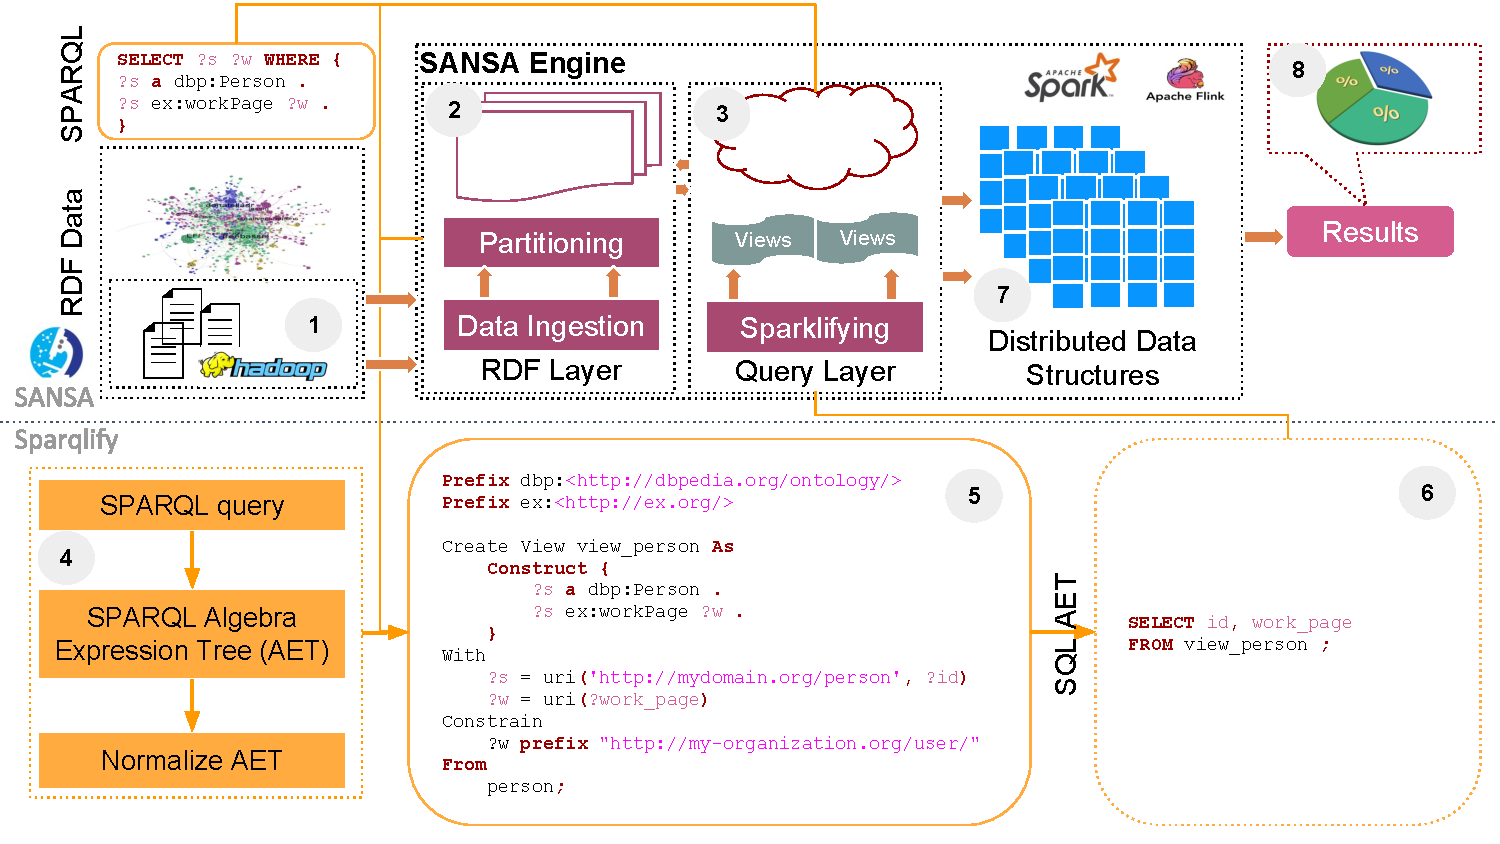
\includegraphics[width=1.0\textwidth]{images/sparklify-architecture.pdf}
\caption{Sparklify Architecture Overview.}
% source : https://docs.google.com/presentation/d/16XlT4u3bFn8XdP_eoLJOAu5WPl_q_9zIjAZbllfEEic/edit?usp=sharing 
\label{fig:architecture}
% source : 
\end{figure*}

\section{Sparklify}
\label{sec:approach}

In this section, we present the overall architecture of our proposed approach, the SPARQL-to-SQL rewriter, and mapping to Spark Scala-compliant code.

\subsection{System Architecture}
The overall system architecture is shown in \autoref{fig:architecture}.
It consists of four main components: Data Model, Mappings, Query Translator and Query Evaluator.
In the following, each component is discussed in details.

\subsubsection{Data Model}
SANSA~\cite{lehmann-2017-sansa-iswc} comes with different data structures and different partitioning strategies.
We model and store RDF graph following the concept of RDDs -- a basic building blocks of the Spark Framework.
RDDs are in-memory collections of records which are capable of operating in parallel overall larger cluster.
Sparklify makes use of SANSA bottom layer which corresponds with the extended vertical partitioning (VP) including RDF terms.
This partition model is the most convenient storage model for fast processing of RDF datasets on top of HDFS.
\paragraph{Data Ingestion (step 1)} RDF data first needs to be loaded into a large-scale storage that Spark can efficiently read from.
We use Hadoop Distributed File-System (HDFS)\furl{https://hadoop.apache.org/docs/r1.2.1/hdfs_design.html}.
Spark employ different data locality scheme in order to accomplish computations nearest to the desired data in HDFS, as a result avoiding i/o overhead. 
\paragraph{Data Partition (step 2)}
VP approach in SANSA is designed to support extensible partitioning of RDF data.
Instead of dealing with a single three-column table $(s, p, o)$, data is partitioned into multiple tables based on the used RDF predicates, RDF term types and literal datatypes.
The first column of these tables is always a string representing the subject.
The second column always represents the literal value as a Scala/Java datatype.
Tables for storing literals with language tags have an additional third string column for the language tag.
\subsubsection{Mappings/Views}
After the RDF data has been partitioned using the extensible VP (as it has been described on \textit{step 2}) the relational-to-RDF mapping is performed. 
Sparqlify supports both the W3C standard R2RML
sparqlification~\cite{sml}.

The main entities defined with SML are \textit{view definitions}.
See \textit{step 5} in the \autoref{fig:architecture} as an example.
The actual view definition is declared by the \emph{Create View} \ldots \emph{As} in the first line.
The remainder of the view contains these parts: (1) the \emph{From} directive defines the logical table based on the partitioned table (see \textit{step 2}).
(2) an RDF template is defined in the \emph{Construct} block containing, URI, blank node or literals constants (e.g. \emph{ex:worksAt}) and variables (e.g. \emph{?emp}, \emph{?institute}).
The \emph{With} block defines the variables used in the template by means of RDF term constructor expressions whose arguments refer to columns of the logical table.

\subsubsection{Query Translation}
This process generates a SQL query from the SPARQL query using the bindings determined in the mapping/view construction phases.
It walks through the SPARQL query (\textit{step 4}) using Jena ARQ\furl{https://jena.apache.org/documentation/query/} and generates the SPARQL Algebra Expression Tree (AET). Essentially, rewriting SPARQL basic graph patterns and filters over views yields AETs that are UNIONS of JOINS.
%AET are .... \fixme{Gezim: complete the sentence}
Further, these AETs are normalized and pruned in order to remove UNION members that are known to yield empty results, such as joins based on IRIs with disjoint sets of known namespaces, or joins between different RDF term types (e.g. literal and IRI).
Finally, the SQL is generated (\textit{step 6}) using the bindings corresponding to the views (\textit{step 5}).

\subsubsection{Query Evaluator}
The SQL query created as described in the previous section can now be evaluated directly into the Spark SQL engine.
The result set of this SQL query is distributed data structure of Spark (e.g. DataFrame)(\textit{step 7}) which then is mapped into a SPARQL bindings.
The result set can further used for analysis and visualization using the SANSA-Notebooks (\textit{step 8})~\cite{iermilov-2017-sansa-iswc-demo}.

\subsection{Algorithm Description}
\label{subsection:algorithm}
The algorithm described in this paper has been implemented using the Apache Spark framework (see \autoref{alg:sparklify}). 
It constructs the graph (\autoref{line:sparklify_rdf2rdd}) while reading RDF data and converts it into RDD of triples.
After, it partitions the data (\autoref{line:sparklify_partitiongraph}, for more details see \autoref{alg:partitionGraph}) using the vertical partitioning (VP) strategy.
Finally, the query evaluator is constructed (\autoref{line:sparklify_sparql}) which is described into more details in \autoref{alg:sparql} for consistency.

\begin{algorithm}[t]
\caption{Sparklify algorithm.}
\label{alg:sparklify}
\SetKwInOut{Input}{input}\SetKwInOut{Output}{output}
\Input{$q$: a SPARQL query, $input$: an RDF dataset}
\Output{$df$ list of result set}
    $\textit{graph} = spark.\textbf{rdf}(lang)(input)$ \label{line:sparklify_rdf2rdd}\\
    $\textit{graph}.persist()$\\
    $partitionGraph \leftarrow graph.\textbf{partitionGraph}()$ \label{line:sparklify_partitiongraph}\\
    $result \leftarrow partitionGraph.\textbf{sparql}(q)$ \label{line:sparklify_sparql}\\
\Return{$result$}
\end{algorithm}

\subsubsection{Partitioning the Graph}
The partitioning algorithm (see \autoref{alg:partitionGraph}) transforms the RDF graph into a convenient VP including RDF terms (\autoref{line:partitionGraph_partitioner}).
For each triple in the graph in a distributed fashion, it does the following: It gets the RDF terms about subjects and objects (\autoref{line:partitionGraph_RDFTerms}).
In case of a literal it assigns the data type for a given column while partitioning the data to: \textit{String} (\autoref{line:partitionGraph_isString}) when is plain literal, otherwise gets the data type of a given literal (e.g. \textit{Integer}, \textit{Double}) (\autoref{line:partitionGraph_LiteralDatatype}).
The remaining block is the language tag (\autoref{line:partitionGraph_languageTag}) which is required for an extra column on the partitioned table containing the language tag value.
After all this information is populated, the partitioned block is performed using the \emph{map} transformation function of Spark splitting the tables based on the above information.

\begin{algorithm}[t]
\caption{PartitionGraph algorithm.}
\label{alg:partitionGraph}
\SetKwInOut{Input}{input}\SetKwInOut{Output}{output}
\Input{$graph$: an RDD[Triple] dataset}
\Output{$views$ a mapped views}
    \ForEach{$triple \in graph$}{
        $s \leftarrow triple.getSubject; o \leftarrow triple.getObject$\\
        $subjectType \leftarrow getRDFTermType(s); objectType \leftarrow getRDFTermType(o)$ \label{line:partitionGraph_RDFTerms}\\
        $predicate \leftarrow triple.getPredicate.getURI$\\
        \eIf{o.isLiteral}{
        \eIf{isPlainLiteral(o)}{
            $datatype \leftarrow XSD.xstring.getURI$ \label{line:partitionGraph_isString}
            }{
            $datatype \leftarrow o.getLiteralDatatypeURI$ \label{line:partitionGraph_LiteralDatatype}
            }}{
        $datatype \leftarrow string.Empty$
        }
        $langTagPresent \leftarrow isPlainLiteral(o)$ \label{line:partitionGraph_languageTag} \\
        $views.add(partitioner(subjectType,predicate, objectType, datatype,$ \label{line:partitionGraph_partitioner} \\ $\quad \quad \quad \quad \quad langTagPresent))$
        }
\Return{$views$}
\end{algorithm}

\subsubsection{Querying the Graph}
Given a SPARQL query and a set of partitions together with associated RDDs, Sparklify
first has to create OBDA view definitions from the partitions (\autoref{line:sparql_vd}) and register their corresponding RDDs with names that can be referenced from Spark SQL (\autoref{line:register-vd}). Hence, the algorithm collects the schema (\autoref{line:sparql_schema}) and constructs a logical table name (\autoref{line:sparql_tn}) based on the partitions.
%Sparqlify is able to rewrite (\autoref{line:sparql_rewriter}) the algebra expressions based on the mappings and generate the view definition about such expressions.
The final step is to create a Spark data frame (\autoref{line:sparql_df}) from the SQL query that is part of the rewrite object generated by Sparqlify (\autoref{line:sparql_sql}).

   %$ers \leftarrow Sparqlify.createDefaultExprRewriteSystem()$\\
%   $mappingOps \leftarrow %Sparqlify.createDefaultMappingOps(ers)$\\
\begin{algorithm}[t]
\caption{sparql algorithm.}
\label{alg:sparql}
\SetKwInOut{Input}{input}\SetKwInOut{Output}{output}
\Input{views: a Map[partition, RDD[Row]] views, $q$: a SPARQL query}
\Output{$df$ a data frame with the rewritten SPARQL query's result set}
    $vds \leftarrow emptyList()$\\
    \ForEach{$(v, rdd) \in views$}{
        $vd \leftarrow Sparqlify.createViewDefinition(v)$ \label{line:sparql_vd}\\
         $tableName \leftarrow vd.logicalTableName$ \label{line:sparql_tn}\\
         $scalaSchema \leftarrow v.layout.schema$\\
         $sparkSchema \leftarrow ScalaReflection.schemaFor(scalaSchema).dataType$ \label{line:sparql_schema}\\
         $df \leftarrow spark.createDataFrame(rdd, sparkSchema)$\\
         $df.createOrReplaceTempView(vd.logicalTableName)$\label{line:register-vd}\\
         $vds.add(vd)$\\
    }
    $rewriter \leftarrow Sparkqlify.createDefaultSparqlSqlStringRewriter(vds)$ \label{line:sparql_rewriter}\\
    $rewrite \leftarrow rewriter.rewrite(q)$\\
$sqlQueryStr \leftarrow rewrite.sqlQueryString$ \label{line:sparql_sql}\\
 %  $sqlQueryStr \leftarrow rewriter.getSqlQueryString$\\  $sqlQueryStr \leftarrow rewriter.getSqlQueryString$ \label{line:sparql_sql}\\
  $df \leftarrow spark.sql(sqlQueryStr)$ \label{line:sparql_df}\\
         
\Return{$df$}
\end{algorithm}

\section{Evaluation}
\label{sec:evaluation}

The goal of our evaluation is to observe the impact of the extensible VP as well as analyzing its scalability when the size of the datset increases.
At the same time, we also want to measure the effect of using Sparqlify optimizer for improving the query performance.
Especially, we want to verify and answer the following questions:
\begin{itemize}
\addtolength{\itemindent}{1cm}
   %\newitem[Q1]\label{item:Q1}: What impact plays the extensible VP? \fixme{Gezim: Not sure if we can cover this analysis, even though would be great to have when I added it here. We can comment it out for now.}
    \newitem[Q1]\label{item:Q1}: Is the runtime affected when more nodes are added in the cluster?
    \newitem[Q2]\label{item:Q2}: Does it scale to a larger dataset?
    \newitem[Q3]\label{item:Q3}: How does it scale when adding a larger number of datasets?
\end{itemize}
In the following, we present our experiments setting including the benchmarks used and server configurations. 
Afterword, we elaborate on our findings.

\subsection{Experimental Setup}
We used two well-known SPARQL benchmarks for our evaluation. 
The \textit{Lehight University Benchmak (LUBM)} v3.1~\cite{Guo2005LUBMAB} and \textit{Waterloo SPARQL Diversity Test Suite (WatDiv)} v0.6~\cite{Alu2014DiversifiedST}.
Characteristics of the considered datasets are given in \autoref{tab:dataset_info}.

\textit{LUBM} comes with a \textit{Data Generator (UBA)} which generates synthetic data over the \textit{Univ-Bench} ontology in the unit of a university.
Our \textit{LUBM} datasets consist of 1000, 5000, and 10000 universities.
The number of triples varies from 138M for 1000 universities, to 1.4B triples for 10000 universities.
\textit{LUBM}'s test suite is comprised of 14 queries. %provides a Test Queries, more specifically 14 test queries.

We have used \textit{WatDiv} datasets with approximate 10K to 1B triples with scale factors 10, 100 and 1000, respectively. 
\textit{WatDiv} provides a test suite with different query shapes, therefore, it allows us to compare the performance of Sparklify and the other approach we compare with in a more compact way.
We have generated these queries using the \textit{WatDiv Query Generator} and report the average mean runtime in the overall results presented below.
It comes with a set of 20 predefined query templates so-called \textit{Basic Testing Use Case} which is grouped into four categories, based on the query shape : \textit{star (QS)}, \textit{linear (QL)}, \textit{snowflake (QF)}, and \textit{complex (QC)}.


%with these characteristics (dataset vary from one to three million products)  containing 1000 to 3000 universities.

\begin{table*}
\centering
\begin{tabularx}{\textwidth}{Xccccccc}	
\toprule
\multirow{2}{*}{$\longrightarrow$} & \multicolumn{3}{c|}{LUBM} & \multicolumn{4}{c}{Watdiv} \\
\cline{2-8}  \rule{0pt}{10pt}
&   \scriptsize{1K} & \scriptsize{5K} & \scriptsize{10K}  & \scriptsize{10M} &\scriptsize{100M} &\scriptsize{1B} &\\
\midrule
\scriptsize{\#nr. of triples}& \scriptsize{138,280,374} & \scriptsize{690,895,862} & \scriptsize{1,381,692,508} & \scriptsize{10,916,457} & \scriptsize{108,997,714} & \scriptsize{1,099,208,068} &  \\
\scriptsize{size (GB)}  & \scriptsize{24} & \scriptsize{116} & \scriptsize{232} & \scriptsize{1.5} &\scriptsize{15} &\scriptsize{149} &\\
\bottomrule
\end{tabularx}
{\caption{Summary information of used datasets (nt format).}\label{tab:dataset_info}}
\end{table*}

%\fixme{Once the Table~\ref{tab:dataset_info} would be finished, let's write few lines about the datasets.}

We implemented Sparklify using Spark-2.4.0, Scala 2.11.11, Java 8, and Sparqlify 0.8.3 and all the data were stored on the HDFS cluster using Hadoop 2.8.0.
All experiments were carried out on a commodity cluster of 7 nodes (1 master, 6 workers): Intel(R) Xeon(R) CPU E5-2620 v4 @ 2.10GHz (32 Cores), 128 GB RAM, 12 TB SATA RAID-5, connected via a Gigabit network.
The experiments have been executed three times and the average runtime has been reported into the results.

\subsection{Results}
We evaluate Sparklify using the above datasets and compare it with the chosen state-of-the-art distributed SPARQL query evaluator.
%Due to the space limit
Since our approach does not involve any pre-processing of the RDF data before being able to evaluate SPARQL queries on it, Sparklify is thereby closer to the so-called direct evaluators.
Indeed, Sparklify only needs to virtually partition the data prior.
As a consequence, we omit other distributed evaluators (such as e.g. S2RDF~\cite{Schatzle:2016:SRQ:2977797.2977806}) and compare it with SPARQGX~\cite{sparqlgx-iswc-2016} as it outperforms other approaches as noted by Graux et.al~\cite{sparqlgx-iswc-2016}.
We compare our approach with \emph{SPARQLGX}'s direct evaluator named SDE and report the loading time for partitioning and query execution time, see \autoref{tbl:performance-analysis}.
We specify ``fail'' whenever the system fails to complete the task and ``n/a'' when the task could not be completed due to a failure in one of the intermediate phase.
In some cases e.g. in \autoref{tbl:performance-analysis}, \textit{QC in Watdiv-1B} dataset, we define "partial fail" due to the failure of one of the queries, therefore the sum-up is not possible.

Findings of the experiments are depicted in \autoref{tbl:performance-analysis}, \autoref{fig:sizeup-scalability}, \autoref{fig:node-scalability}, and  \autoref{fig:overall-analysis}.

To verify \ref{item:Q1}, we analyze the \textit{speedup} and compare it with SPARQLGX.
We run the experiments on three datasets, \emph{Watdiv-10M}, \emph{Watdiv-1B} and \emph{LUBM-10K}.
%with two scenarios: (1) while caching the whole datasets and (2) without.

\begin{table*}[t]
\centering
\begin{tabularx}{\textwidth}{*{6}{X}}	
\toprule
\multicolumn{1}{l}{}& \multicolumn{4}{c}{\scriptsize{Runtime (s)} (\scriptsize{mean})} \\
\cline{2-5}
\rule{0pt}{8pt}
\multirow{2}{*}{$\longrightarrow$} & \multicolumn{1}{c|}{\scriptsize{\textbf{SPARQLGX-SDE}}} & \multicolumn{3}{c}{\scriptsize{\textbf{Sparklify}}} \\
\cline{2-5}  \rule{0pt}{10pt}
& \scriptsize{a) total} & \scriptsize{b) paritioning}  & \scriptsize{c) querying} & \scriptsize{d) total} \\
\midrule
\multirow{5}{*}{\rotatebox{90}{\scriptsize{\textbf{Watdiv-10M}}}}
&  & & & \\
\hspace{0.2cm} $QC$ & \win \scriptsize{103.24} & \scriptsize{134.81} & \win \scriptsize{61} & \scriptsize{195.84} \\
\hspace{0.2cm} $QF$ & \win \scriptsize{157.8} & \scriptsize{241.24} & \win \scriptsize{107.33} & \scriptsize{349.51}  \\
\hspace{0.2cm} $QL$ & \win \scriptsize{102.51} & \scriptsize{236.06} & \scriptsize{134} & \scriptsize{370.3} \\
\hspace{0.2cm} $QS$ & \win \scriptsize{131.16} & \scriptsize{237.12} & \win \scriptsize{108.56} & \scriptsize{346} \\
\midrule
\multirow{5}{*}{\rotatebox{90}{\scriptsize{\textbf{Watdiv-1B}}}}
&  & & &  \\
\hspace{0.2cm} $QC$ & \textcolor{red}{\scriptsize{partial fail} }& \win \scriptsize{778.62} & \win \scriptsize{2043.66} & \win \scriptsize{2829.56} \\
\hspace{0.2cm} $QF$ & \scriptsize{6734.68} & \win \scriptsize{1295.31} & \win \scriptsize{2576.52} & \win \scriptsize{3871.97} \\
\hspace{0.2cm} $QL$ & \scriptsize{2575.72} & \win \scriptsize{1275.22} & \win \scriptsize{610.66} & \win \scriptsize{1886.73} \\
\hspace{0.2cm} $QS$ & \scriptsize{4841.85} & \win \scriptsize{1290.72} & \win \scriptsize{1552.05} & \win \scriptsize{2845.3} \\
\midrule
%\multirow{14}{*}{\rotatebox{90}{\scriptsize{\textbf{LUBM-1K}}}}
%$Q1$ & \scriptsize{..} & \scriptsize{99.92} & \scriptsize{5.74} &  \scriptsize{105.66} &  \scriptsize{n/a\textbar56.4x}\\
%\hspace{0.2cm} $Q2$ & \scriptsize{..} & \scriptsize{88.68} & \scriptsize{3842.6} & \scriptsize{3932.35} & \scriptsize{n/a\textbar56.4x}\\
%\hspace{0.2cm} $Q3$ & \scriptsize{..} & \scriptsize{80.91} & \scriptsize{18.11} & \win \scriptsize{99.03} & \scriptsize{n/a\textbar56.4x}\\
%\hspace{0.2cm} $Q4$ & \scriptsize{..} & \scriptsize{101.98} & \scriptsize{27.6} & \win \scriptsize{129.64} & \scriptsize{n/a\textbar56.4x}\\
%\hspace{0.2cm} $Q5$ & \scriptsize{..} & \scriptsize{97.62} & \scriptsize{18.6} &  \scriptsize{116.3} & \win \scriptsize{n/a\textbar56.4x}\\
%\hspace{0.2cm} $Q6$ & \scriptsize{..} & \scriptsize{99.88} & \scriptsize{15.92} & \win \scriptsize{115.86} & \win \scriptsize{n/a\textbar56.4x}\\
%\hspace{0.2cm} $Q7$ & \scriptsize{..} & \scriptsize{100.28} & \scriptsize{26.85} & \scriptsize{127.2} & \scriptsize{n/a\textbar56.4x}\\
%\hspace{0.2cm} $Q8$ & \scriptsize{..} & \scriptsize{91.31} & \scriptsize{26.69} & \scriptsize{118.06} & \scriptsize{n/a\textbar56.4x}\\
%\hspace{0.2cm} $Q9$ & \scriptsize{..} & \scriptsize{96.25} & \scriptsize{31.16} & \win \scriptsize{..} & \win \scriptsize{n/a\textbar56.4x}\\
%\hspace{0.2cm} $Q10$ & \scriptsize{..} & \scriptsize{97.9} & \scriptsize{19.41} & \win \scriptsize{117.33} & \win \scriptsize{n/a\textbar56.4x}\\
%\hspace{0.2cm} $Q11$ & \scriptsize{..} & \scriptsize{99.69} & \scriptsize{17.72} &  \scriptsize{117.49} &  \scriptsize{n/a\textbar56.4x}\\
%\hspace{0.2cm} $Q12$ & \scriptsize{..} & \scriptsize{96.87} & \scriptsize{22.43} & \win \scriptsize{119.32} & \win \scriptsize{n/a\textbar56.4x}\\
%\hspace{0.2cm} $Q13$ & \scriptsize{..} & \scriptsize{102.16} & \scriptsize{8.58} & \win \scriptsize{110.78} &  \scriptsize{n/a\textbar56.4x}\\
%\hspace{0.2cm} $Q14$ & \scriptsize{..} & \scriptsize{95.83} & \scriptsize{15.19} & \win \scriptsize{111.16} & \win \scriptsize{n/a\textbar56.4x}\\
%\midrule
\multirow{14}{*}{\rotatebox{90}{\scriptsize{\textbf{LUBM-10K}}}}
$Q1$ & \win \scriptsize{1056.83} & \scriptsize{627.72} & \scriptsize{718.11} & \scriptsize{1346.8}\\
\hspace{0.2cm} $Q2$ & \textcolor{red}{\scriptsize{fail}} & \scriptsize{595.76} & \textcolor{red}{\scriptsize{fail}} &  \scriptsize{n/a} \\
\hspace{0.2cm} $Q3$ & \win \scriptsize{1038.62} & \scriptsize{615.95} & \scriptsize{648.63} &  \scriptsize{1267.37} \\
\hspace{0.2cm} $Q4$ & \scriptsize{2761.11} & \win \scriptsize{632.93} & \win \scriptsize{1670.18} &  \win \scriptsize{2303.18} \\
\hspace{0.2cm} $Q5$ & \win \scriptsize{1026.94} & \scriptsize{641.53} & \scriptsize{564.13} &  \scriptsize{1206.67}\\
\hspace{0.2cm} $Q6$ & \win \scriptsize{537.65} & \scriptsize{695.74} & \scriptsize{267.48} &  \scriptsize{963.62}\\
\hspace{0.2cm} $Q7$ & \scriptsize{2080.67} & \win \scriptsize{630.44} & \win \scriptsize{1331.13} &  \win \scriptsize{1967.25}\\
\hspace{0.2cm} $Q8$ & \scriptsize{2636.12} & \win \scriptsize{639.93} & \win \scriptsize{1647.57} &  \win \scriptsize{2288.48} \\
\hspace{0.2cm} $Q9$ & \scriptsize{3124.52} & \win \scriptsize{583.86} & \win \scriptsize{2126.03} &  \win \scriptsize{2711.24} \\
\hspace{0.2cm} $Q10$ & \win \scriptsize{1002.56} & \scriptsize{593.68} & \scriptsize{693.73} &  \scriptsize{1287.71} \\
\hspace{0.2cm} $Q11$ & \win \scriptsize{1023.32} & \scriptsize{594.41} & \scriptsize{522.24} &  \scriptsize{1118.58}\\
\hspace{0.2cm} $Q12$ & \scriptsize{2027.59} & \win \scriptsize{576.31} & \win \scriptsize{1088.25} &  \win \scriptsize{1665.87} \\
\hspace{0.2cm} $Q13$ & \scriptsize{1007.39} & \win \scriptsize{626.57} & \win \scriptsize{6.66} &  \win \scriptsize{633.26} \\
\hspace{0.2cm} $Q14$ & \win \scriptsize{526.15} & \scriptsize{633.39} & \scriptsize{258.32} &  \scriptsize{891.89}\\
\bottomrule
\end{tabularx}
{\caption{Performance analysis on large-scale RDF datasets.}\label{tbl:performance-analysis}}
\end{table*} %source : https://docs.google.com/spreadsheets/d/16CcsZcmrGF0yevu8L5mlAALGB2JZvHNkS4-6WQV0edo/edit?usp=sharing

\autoref{tbl:performance-analysis} shows the performance analysis of two approaches run on three different datasets.
Column SPARQLGX-SDE$^{a}$ reports on the performance of SPARQLGX-SDE considering the total runtime to evaluate the given queries.
Column Sparklify$^{b}$ lists the times required for Sparklify to perform the VP and then the query execution time is reported on the Sparklify$^{c}$.
Total runtime for Sparklify is shown in the last column, Sparklify$^{d}$.

We observe that the execution of both approaches fails for the \textit{Q2} in the \textit{LUBM-10K} dataset while evaluating the query. 
We believe that it is due to the reason that \textit{LUBM Q2} involves a triangular pattern which is often resource consuming. 
As a consequence, in both cases, Spark performs the shuffling (e.g. data scanning) while reducing the result set.
It is interesting to note that for the \textit{Watdiv-1B} dataset, SPARQLGX-SDE fails for the query \textit{C3} when data scanning is performed. 
Sparklify is capable of evaluating it successfully.
Due to the Spark SQL optimizer in conjunction with Sparqlify's approach of rewriting a SPARQL query typically into only a single SQL query -- effectively offloading all query planning to Spark -- Sparklify performs better than SPARQLGX-SDE when the size of the dataset increases (see \textit{Watdiv-1B results} in the \autoref{tbl:performance-analysis}) and when there are more joins involved (see \textit{Watdiv-1B} and \textit{LUBM-10K} results in the \autoref{tbl:performance-analysis}).
SPARQLGX-SDE evaluates the queries faster when the size of the datasets is smaller, but it degrades when the size of the dataset increases.
The likely reason for Sparklify's worse performance on smaller datasets is its higher partitioning overhead.
\autoref{fig:sizeup-scalability} shows that Sparklify starts outperforming when the size of the datasets grows (e.g. \textit{Watdiv-100M}).

\begin{figure}
 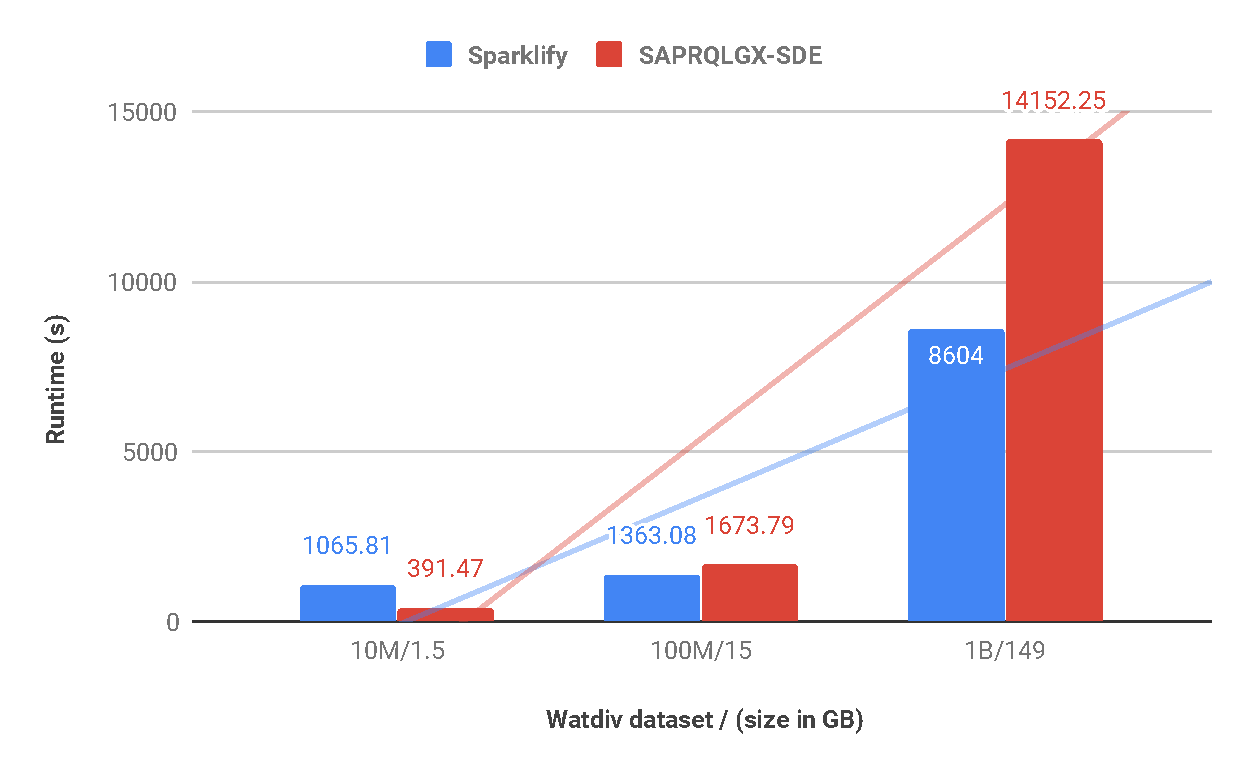
\includegraphics[width=1.0\columnwidth]{images/sizeup-scalability.pdf}
    \caption{Sizeup analysis (on Watdiv dataset).}
    \label{fig:sizeup-scalability}
\end{figure}

\defn{Size-up scalability analysis}
To measure the performance of the data scalability (e.g. size-up) of both approaches, we run experiments on three different sizes of \textit{Watdiv} (see \autoref{fig:sizeup-scalability}).
We keep the number of nodes constant i.e 6 worker nodes and grow the size of the datasets to measure whether both approaches can deal with larger datasets.
We see that the execution time for Sparklify grows linearly compared with SPARQLGX-SDE, which keeps staying as near-linear when the size of the datasets increases. 
The results presented show scalability of Sparklify in context of the sizeup, which addresses the question \ref{item:Q2}.

\defn{Node scalability analysis}
To measure the node scalability of Sparklify, we vary the number of worker nodes.
We vary them from 1, 3 to 6 worker nodes.
\autoref{fig:node-scalability} depict the speedup performance of both approaches run on \textit{Watdiv-100M} datasaet when the number of worker nodes varies.
We can see that as the number of nodes increases, the runtime cost for the Sparklify decrease linearly.
The execution time for Sparklify decreases about 0.6 times (from 2547.26 seconds down to 1588.4 seconds) as worker nodes increase from one to three nodes.
We see that the speedup stays constant when more worker nodes are added since the size of the data is not that large and the network overhead increases a little the runtime when it runs over six worker nodes.
This imply that our approach is efficient up to three worker nodes for the \textit{Watdiv-100M} (15GB) dataset.
In another hand, SPARQLGX-SDE takes longer to evaluate the queries when running on one worker node but it improves when the number of worker nodes increases.
%... \fixme{Gezim: finish this when the results are out.}

Result presented here shows that Sparklify can achieve linear scalability in the performance, which addresses \ref{item:Q3}.

\begin{figure}
  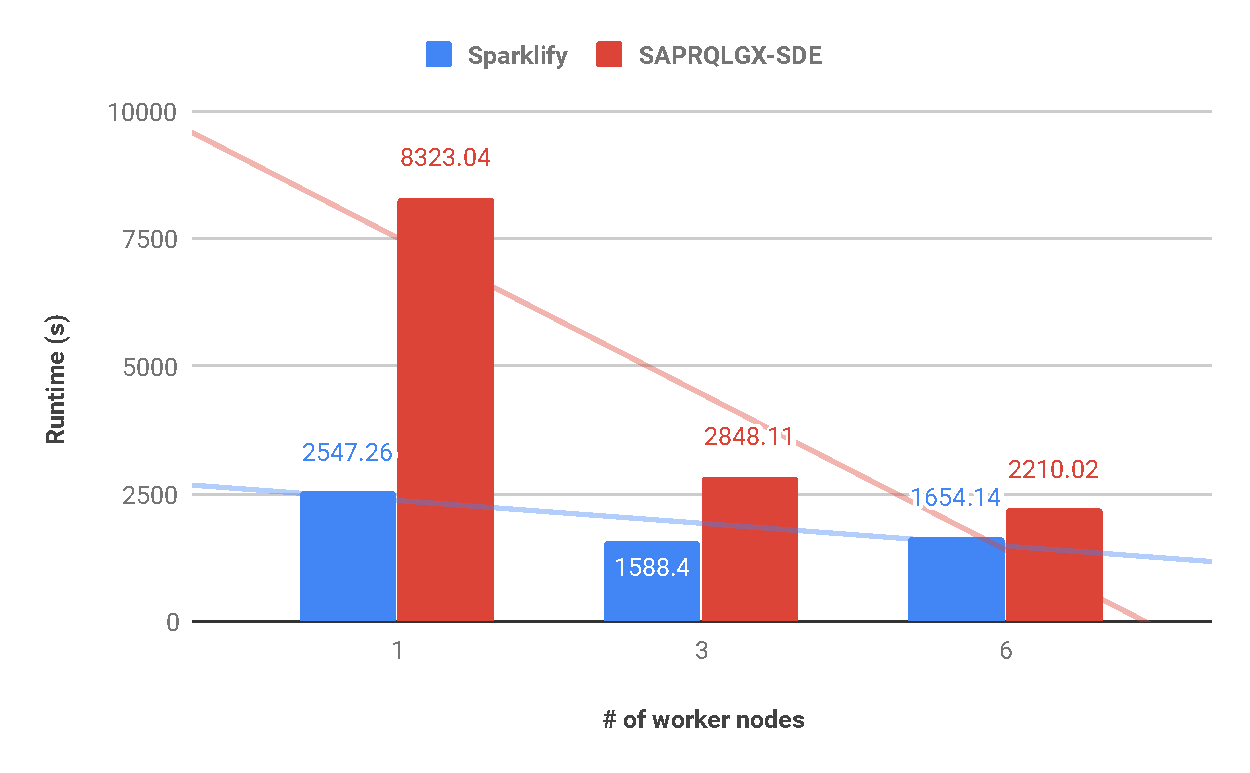
\includegraphics[width=1.0\columnwidth]{images/node-scalability.pdf}
    \caption{Node scalability (on Watdiv-100M).}
    \label{fig:node-scalability}
\end{figure}

\defn{Correctness of the result set}
In order to assess the correctness of the result set, we computed the count of the result set for the given queries and compare it within both approaches.
We conclude that both approaches return exactly the same result set which implies the correctness of the results.


\defn{Overall analysis by SPARQL queries}
Here we analyze Watdiv queries run on \textit{Watdiv-100M} dataset in a cluster mode on both approaches.
%\fixme{Gezim: Complete this part and analyze the queries which take longer for SDE on large datasets and those with takes longer for Sparklify on medium datasets.}

\begin{figure}
  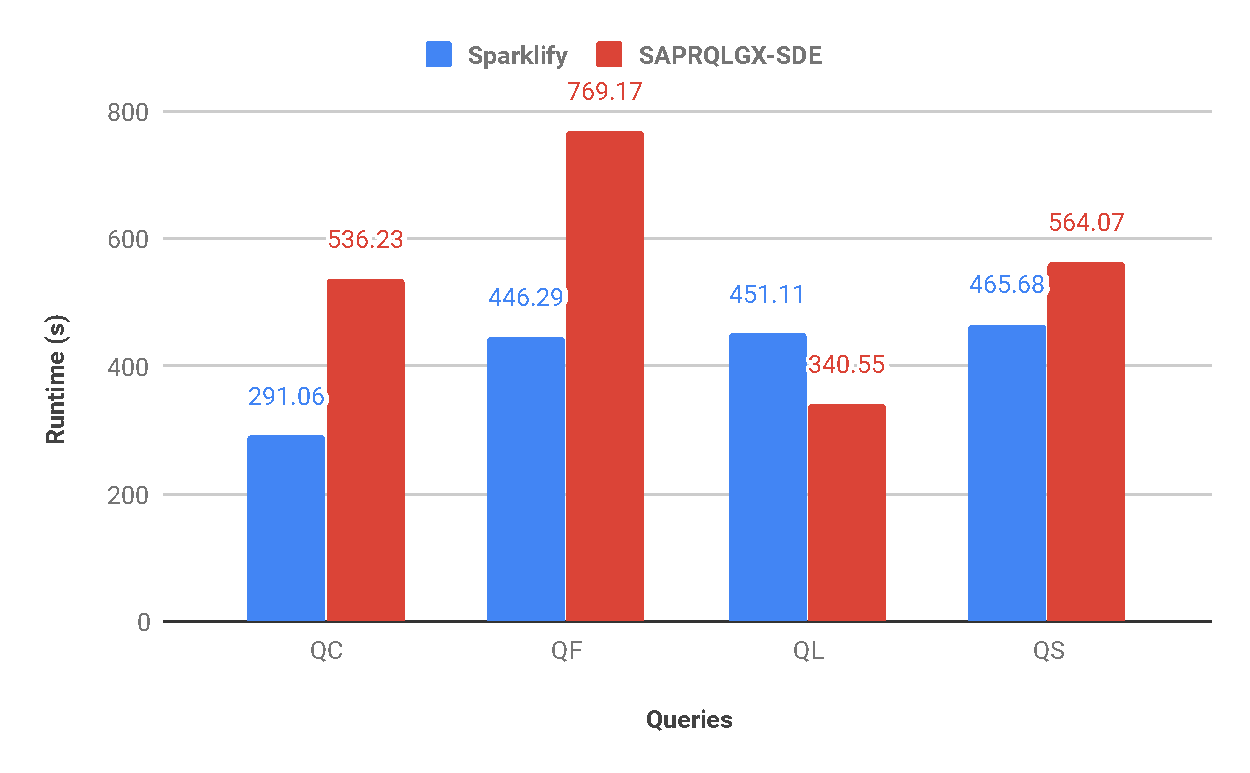
\includegraphics[width=1.0\columnwidth]{images/overall-analysis.pdf}
    \caption{Overall analysis of queries on Watdiv-100M dataset (cluser mode).}
    \label{fig:overall-analysis}
\end{figure}

%\strut\\
%\textcolor{orange}{
%    \noindent
%    Here are some ideas of discussion about the results:
%    \begin{itemize}
%        \item SDE seems not to be less performance as the number of TPs involved i the query increase. This might be due to the fact that SDE has to read the whole triple file each time.
%    \end{itemize}
%}

According to \autoref{fig:overall-analysis}, SPARQLGX-SDE performance decreases as the number of triple patterns involved in the query increase. %As it is depicted in the \autoref{fig:overall-analysis}, SPARQLGX-SDE seems to be less performance as the number of triple patterns involved in the query increase. 
This might be due to the fact that SPARQLGX-SDE has to read the whole triple file each time.
In contrast to SPARQLGX-SDE, Sparklify seems to perform well when there are more triple pattern involved (see queries \textit{QC}, \textit{QF} and \textit{QS} in the \autoref{fig:overall-analysis}) but slightly worst when there are linear queries (see \textit{QL}) evaluated. 
This may be due to the reason that Sparqlify typically rewrites a SPARQL query into a single SQL query, thus maximizing the opportunities given to the Spark SQL optimizer. Conversely, SPARQLGX-SDE constructs the workflow by chaining Scala API calls, which may restrict the possibilities e.g. in regard to join ordering.
Based on our findings and the evaluation study carried out in this paper, we show that Sparklify is scalable and the execution time ends in a reasonable time given the size of the dataset.

\section{Use Cases} 
\label{sec:use_cases}
%\fixme{Gezim: Complete this section.}

Sparklify, as a default query engine for SANSA has been used in different major use cases. 
Below, we list some of them that we are aware of using Sparklify:

\defn{Blockchain -- Alethio Use Case} Alethio\furl{https://aleth.io/} try to present the big picture of the whole Ethereum ecosystem.
It is a powerful blockchain data, analytics, and visualisation platform.
It contains more than 18 Billion triples datasets ``rdfized'' using the structure of the Ethereum ontology\furl{https://github.com/ConsenSys/EthOn}.
They are taking advantage of the SANSA stack by querying this amount of data at scale e.g. analyzing the Hubs \& Authorities in the Ethereum Transaction Network\furl{https://bit.ly/2YX7CXG} and other analytics.

\defn{SPECIAL -- A Semantic Transparency and Compliance Use Case}
SPECIAL\furl{https://www.specialprivacy.eu} is a Scalable Policy-aware Linked Data platform for privacy, transparency, and compliance.
Within the project, they introduce SPIRIT -- a transparency and compliance checking implementation of the SANSA stack.
SPECIAL uses SANSA engine in order to analyze the log information concerning personal data processing and sharing that as an output from line of business applications on a continuous basis, and to present the information to the user via the SPIRIT dashboard.
The SPIRIT transaction log processing allows users to: (1) define the set of policies rules, (2) initialize the query engine with the log and schema/ontology data, here is where Sparklify is used in specific, (3) create a reasoner set reasoning profile, and (4) apply these rules to the given query in order be compliant with the policy rules.

\defn{SLIPO -- Categorizing Areas of Interests (AOI) Use Case} SLIPO\furl{http://slipo.eu/} take advantage of the Semantic Web Technologies for the scalable and efficient integration of Big Point of Interest (POI) datasets.
In particular, the project focuses on designing efficient pipelines dealing with large semantic datasets of POIs: a wide range of features are available inter alia fusion \& cleaning distinct datasets or detection of future ``hot'' AOIs where businesses should be created.
In this project, Sparklify is used through the SANSA query layer to refine, filter and select the relevant POIs which are needed by the pipelines.

%\defn{QROWD -- Something}
%QROWD\furl{http://qrowd-project.eu/} is a cross-sectorial project which offers local government and transportation businesses innovative solutions to improve mobility, reduce traffic congestion and make navigation safer and more efficient. 
%In order to achieve this, QROWD integrate different sources of data by leveraging the value of Big Data processing engine and semantic web technologies.
%One of the challenges to be tackled in QROWD is the disambiguation while crawling the data. 
%\fixme{Gezim-to-Claus: I think you know it better to explain it.}






\section{Related Work}
\label{sec:related_work}

As our main focus is on the area of distributed computing, we omit the centralized systems e.g. RDF-3X~\cite{Neumann2008RRE} or Virtuoso~\cite{Erling2010} (see~\cite{faye2012survey} for a survey) and we review the distributed ones only (see~\cite{kaoudi2015rdf} for a recent survey).
Further, this set of tools is divided into: \textit{MapReduce-based} systems and \textit{In-Memory} systems e.g. on top of Apache Spark.

\textit{MapReduce systems} -- SHARD~\cite{Rohloff2010} is one approach which groups RDF data into a dedicated partition so-called semantic-based partition. 
It groups these RDF data by subject and implements a query engine which iterates through each of the clauses used on the query and performs a query processing.
A MapReduce job is created while scanning each of the triple patterns and generates a single plan for each of the triple pattern which leads to a larger query plan, therefore, it contains too many Map and Reduces jobs.
PigSPARQL~\cite{Schatzle2011PMS} is yet another approach which uses Hadoop based implementation of vertical partitioning for data representation. 
It translated the SPARQL queries into Pig\furl{https://pig.apache.org/} LATIN queries and uses Pig as an intermediate engine.
Another approach which is based on the MapReduce is Sempala~\cite{Schatzle2014Sempala} -- as SPARQL-to-SQL approach on top of Hadoop.
It uses Impala\furl{https://impala.apache.org/} as a distributed SQL processing engine.
Sempala uses a so-called unified vertical partitioning (single property table) in order to boost the star-shaped queries by excluding the joins.
Hence, its limitation is that it is designed only to that particular shape of the queries.
RYA~\cite{Punnoose2012Rya} is a Hadoop based scalable RDF store that uses Accumulo\furl{https://accumulo.apache.org} as a distributed key-value store for indexing the RDF triples.
RYA indexes triples into three tables and replicate them across the cluster for leveraging the indexes over all the possible records.
It has the mechanism of performing join reorder, but it lacks of the in-memory computation, which makes it not comparable with other systems.
While the MapReduce paradigm has been realized for disk-based as well as in-memory processing, the concept is not concerned with controlling aspects of general distributed workflows, such as which intermediate results to cache. As a consequence, high level frameworks were devised which may use MapReduce as a building block.%The drawback of using the MapReduce paradigm is the usage of the disk-based processing, therefore, the new solution came out.
Apache Spark is one of them~\cite{zaharia2012resilient}.
Below, we will list some of the approaches which make use of the Apache Spark (in-memory computation) framework. 

\textit{In-Memory systems} --
SPARQLGX~\cite{sparqlgx-iswc-2016} and S2RDF~\cite{Schatzle:2016:SRQ:2977797.2977806} approaches are considered the most recent distributed SPARQL evaluators over large-scale RDF datasets.
SPARQLGX is a scalable query engine which is capable of evaluating efficiently the SPARQL queries over distributed RDF datasets~\cite{graux2018multi}.
It provides a mechanism for translating SPARQL queries into Spark executable code for better leveraging the advantage of the Spark framework.
It uses a simplified VP approach, where each predicate is assigned with a specific parquet file. 
As an addition, it is able to assign RDF statistics for further query optimization while also providing the possibility of directly query files on the HDFS using SDE.
S2RDF is similar to SPARQLGX, but instead of dealing with direct Spark code (aka RDDs), it translates SPARQL queries into SQL ones run by Spark-SQL. 
It introduces a data partitioning strategy that extends VP with additional statistics, containing pre-computed semi-joins for query optimization.


\section{Conclusions and Future Work}
\label{sec:conclusion}
Querying RDF data becomes challenging when the size of the data increases.
%Existing systems mostly contain a very moderately information of the data while transforming them to a dedicated storage model (e.g. vertical partitioning).
%contain a very moderately information of the data
Existing Spark-based SPARQL systems mostly
do not retain all RDF term information consistently while transforming them to a dedicated storage model such as using vertical partitioning.
Often, this process is both data and computing intensive and raises the need for a scalable, efficient and comprehensive query engine which can handle large scale RDF datasets.

In this paper, we propose \emph{Sparklify}: a scalable software component for efficient evaluation of SPARQL queries over distributed RDF datasets. 
It uses Sparqify as a SPARQL-to-SQL rewriter for translating SPARQL queries into Spark executable code.
By doing so, it leverages the advantages of the Spark framework.
SANSA features methods to execute SPARQL queries directly as part of Spark workflows instead of writing the code corresponding to those queries (sorting, filtering, etc.).
It also provides a command-line interface and a W3C standard compliant SPARQL endpoint for externally querying data that has been loaded using the SANSA framework.
We have shown empirically that our approach can scale horizontally and perform well w.r.t to the state-of-the-art approaches.

With this work, we showed that the application of OBDA tooling to Big Data frameworks achieves promising results in terms of scalability. 
We present a working prototype implementation that can serve as a baseline for further research. 
Our next steps include evaluating other tools, such as Ontop~\cite{Calvanese2017OntopAS}, and analyze how their performance in the Big Data setting can be improved further. 
For example, we intend to investigate how OBDA tools can be combined with dictionary encoding of RDF terms as integers and evaluate the effects.

%Although we have achieved %reasonable results in %terms of scalability, we %further plan to cover more %SPARQL fragments.

%\section*{Acknowledgment}
%This work was partly supported by the EU Horizon2020 projects BigDataOcean (GA no.~732310), Boost4.0 (GA no.~780732), SLIPO (GA no.~731581) and QROWD (GA no.~723088); and by the ADAPT Centre for Digital Content Technology funded under the SFI Research Centres Programme (Grant 13/RC/2106) and co-funded under the European Regional Development Fund.

%\bibliographystyle{abbrv}
%\bibliography{references}

%\clearpage 

%{\huge Pages: \the\numexpr\value{page}-1\relax{} (Limit: 16)}

%\end{document}



%\vspace{-5mm}
\section{Introduction}
%\todo{State that the relation between SPARQL and SPIN\url{http://spinrdf.org/}
%is similar to SML and R2RML, respectively. - Jens: not sure whether this should
% be a main point here?}

\begin{comment}
core problem is not ontological but algebraic; makes more sense to introduce a formal model and present mappings/transformations than introducing an ontology for this problem

ontology based access simplified

So far, languages for establishing RDF views on relational data have been based on XML or RDF and therefore lacked the intuitiveness of view definitions in the SQL realm.

Contributions:
\begin{itemize}
 \item formal model for RDB2RDF mappings
 \item language easier to learn than W3C
 \item less errors when writing mappings % falls sich das bei der Eval rausstellt
 \item easier debugging of mappings % besser als bei RDF-basierter Syntax z.B. keine
\end{itemize}

Analogie: Ende 90er wurde RDF/XML eingeführt da XML sehr verbreitet und deshalb als Syntax offensichtlich; analog wurde für R2RML RDF als Syntax verwendet --> in beiden Fällen angepasste Syntax übersichtlicher und leichter zu lernen
\end{comment}

% describe topic / importance
Despite the success of semantic technologies, a large share of structured knowledge still resides in relational databases.
For this reason, significant research effort has been invested by the Semantic Web community into making relational databases available as RDF.

% why: mapping languages drawbacks and advantages
Due to the strong interest in this area, several approaches and languages for mapping relational data to triples have been devised, in particular the W3C standard R2RML\footnote{\url{http://www.w3.org/TR/r2rml/}}.
While having a standard itself is of high importance, we argue that R2RML has some drawbacks on the syntactical level:
Writing RDF views in R2RML is very verbose and arguably not as intuitive as it could be.
%\todo{R4: Where is the foundation for this?
%Has a user study been created, concluding that there hasn't been an uptake of
% R2RML because of the syntax? Are the features of R2RML comparable to other languages that in the past have failed?
%Who claims this? Just the authors? (We should be able to answer this after the
% user study)}
The choice of using RDF as base syntax for R2RML has the advantage that people writing mappings can be expected to know RDF.
However, there is a significant gap between the relational database structure and the structure of the R2RML mapping specifications.
While graphical editors, such as \cite{sengupta2013editing}\cite{pinkel2014partner}, partially mitigate the problem of having to write those mapping definitions, these also have their limitations.
%First, there is a number of productive deployments where an additional component is considered a potential security risk.
%In such an environment it is also likely, that access to the host system is only provided via a text console\todo{Jens: I am not sure that this is a strong argument as you will most likely write the mapping specifications locally and then only tets and slightly refine them on the server.}, effectively hindering the utilization of a graphical frontend.
In particular, they would have to support both, the full feature set of the mapping language while still be efficient to work with and producing human readable output.
%, to cater for the scenarios previously described.
Moreover, in some environments, Web based editors in the spirit of phpmyadmin\footnote{\url{http://www.phpmyadmin.net}} may pose security risks or are not convenient, since many database and RDF experts are simply used to work on text files and textual representations of data and queries.
While they appreciate unobtrusive help, like syntax checking or code completion, a graphical user interface might impose an unfitting work flow, for example when an administrator is used to be able to perform small database related tasks via a command line interface.
In this work, we introduce the Sparqlification Mapping Language (SML) as a human friendly alternative to R2RML.
%To overcome the syntactical issues of R2RML, we introduce the SML mapping language. % in this article.
%To clarify, our intention is not to make R2RML obsolete, instead we propose an alternative syntax.
It is noteworthy, that non-RDF syntaxes for which RDF-based versions exist are commonly used the Semantic Web.
For example, while e.g. OWL ontologies can be written directly in RDF, Manchester OWL Syntax\footnote{\url{http://www.w3.org/TR/owl2-manchester-syntax/}} is a popular and concise alternative used in the primer of the OWL 2 specification itself.
As another example, while SPARQL queries in principle can be written in RDF using the SPIN SPARQL Syntax\footnote{\url{http://spinrdf.org/sp.html}}, it is uncommon to do so unless special use cases demand this.

SML is based on work towards a unified formal model for RDB2RDF mappings.
While it has equal expressiveness to R2RML, it uses a different syntactical approach:
It blends the traditional SQL \texttt{CREATE VIEW} statements with SPARQL \texttt{CONSTRUCT} queries.
Both features can be expected to be familiar to persons working on RDB2RDF data integration and combined provide a more concise syntax than R2RML.
In fact, we believe that for RDF itself, history has shown that the seemingly obvious choice of syntactically building on XML has had several drawbacks and the special purpose language Turtle meanwhile enjoys high popularity for manually crafting and editing RDF documents and Turtle 1.1 became a W3C Proposed Recommendation in 2014.
%\todo{Jörg: If not, R2RML chose ttl over xml for that very reason. Jens: I know. The point is more that RDF initially built on XML as it was popular at the same and later moved to Turtle (special purpose syntax). R2RML initially built on RDF (any serialization format) and later some people may move to SML (special purpose syntax). I think the phrasing is correct, but feel free to improve/clarify if not.}
Similarly, we believe a more intuitive special purpose RDB2RDF mapping language can provide similar benefits.

% how: briefly summarise SML
The research on the syntax of SML builds on a comparison of RDB2RDF mapping languages and a subsequently defined formal model of those languages.
Languages like R2RML and SML are syntactic instances of this formal model.
We use this model to highlight the equivalence between the languages and derive approaches for converting between them.
In particular, this implies that any processor, which can work on the W3C R2RML standard, can also use SML as input and no further implementation effort is required to use SML in combination with a number of RDB2RDF engines.
Our main argument is that SML despite its simplicity provides equal expressiveness and is, therefore, a viable alternative to R2RML.
%\todo{R4: There is no experiments or evidence that supports the claim that SML
% is a viable alternative. This one of the most important claims in the paper, but it is not supported with any evidence at all. }
% contributions
The contributions of the article are as follows:
%\vspace{-5mm}
\begin{itemize}
 \item Definition of the compact SML mapping language with equal expressiveness to R2RML
 \item Comparison of RDB2RDF mapping languages.
 \item A unified formal model of RDB2RDF mapping languages.
 \item Converters from R2RML to SML and vice versa.
 \item Syntax highlighting definition for the editor \emph{vim} and an online
 SML editor with syntax and error highlighting as a demonstrator.
 %\todo{R4: Additionally, the syntax highlighting and SML editor are clearly engineering tasks and not scientific contributions. }
 Although this component is an engineering effort, it contributed to
 the fairness of the user study in terms of providing comparable tool support
 for both R2RML and SML.
\end{itemize}
%\vspace{-5mm}

All tools, demos and the specification of the SML syntax, are available at \url{http://sml.aksw.org}.
%\todo{Jens: currently returns a 404 error}

The remainder of the article is structured as follows:
In~\autoref{sec:mapping-language-review} we review existing RDB2RDF mapping
languages. Subsequently, in~\autoref{sec:model} we present a corresponding
formal model. The SML syntax is introduced in~\autoref{sec:syntax},
whereas \autoref{sec:sml-vs-r2rml} compares it to R2RML.
In \autoref{sec:sml2r2rml} the conversion approach from SML to R2RML is described.
In \autoref{sec:eval}, we describe a user study via a public survey with 46 participants amounting to almost 16 hours of survey completion time.
Finally, we conclude this paper in~\autoref{sec:conclusion}.

%\vspace{-5mm}
\section{RDB2RDF Systems and Mapping \\ Languages Review}
\label{sec:mapping-language-review}
% Introduction

The mapping of \emph{relational databases} (RDB) to the \emph{Resource Description Framework} (RDF) is of keen interest from the inception of the \emph{Semantic Web} as exemplified in~\cite{TBL98}.
The exposition of such previously constrained data allows integration and interlinking with other data on the Web.
Based on this need, multiple tools and approaches emerged.
In an approach for fostering interoperability between those tools, the standardization of the RDB2RDF Mapping Language (R2RML) was initiated by the W3C RDB2RDF working group\footnote{\url{http://www.w3.org/2001/sw/rdb2rdf/}}.


% R2RML
R2RML is defined in \cite{r2rml} as a  mapping language for describing customized mappings of relational data into RDF.
The R2RML specification is accompanied by the Direct Mapping (DM) specification~\cite{directmapping}, describing a standard way of translating a relational database into RDF without the use of a customized mapping definition.
An R2RML mapping definition is represented in RDF using the R2RML vocabulary and serialized in the Terse RDF Triple Language (Turtle).
It can be used to either store converted relational data in an RDF dump file, expose the data as Linked Data or allow querying it via a SPARQL endpoint.
A more general overview of mapping tools for structured sources is given in~\cite{UnbehauenSeCo2012}.
Recent efforts, such as \cite{dimou2014rml}, propose extensions of R2RML for non-relational sources by adding support for the use of e.g. XPath\footnote{\url{http://www.w3.org/TR/xpath-30/}} and JSONPath expressions in the mappings.
In this work we focus on relational data.
%However, as for instance XML, these approaches are still based on creating \emph{intermediate} relations e.g. using XPath\footnote{\url{http://www.w3.org/TR/xpath-30/}} and XQuery\footnote{\url{http://www.w3.org/TR/xquery-30/}}.



% R2RML tools
With the advent of R2RML, vendors took up the standard and either modified their existing tools to additionally support R2RML or created tools fully based on the standard.
In general these tools can be categorized with regards to different dimensions, with the type of data exposition and the mode of querying the underlying database being the most distinctive.
A list of existing R2RML tools is given in~\autoref{tbl:toolcomparison}.
%Examples of Existing R2RML based tools are D2R~\cite{d2rserver}, UltraWrap~\cite{sequeda2013ultrawrap}, Ontop~\cite{rodriguez2013evaluating}, Morph~\cite{priyatna2014formalisation}, SparqlMap~\cite{unbehauen-jist-2012-sparqlmap}.
%Further tools are
These tools have in common that they all allow the exposition as SPARQL endpoint and all employ SPARQL-to-SQL translation.

The R2RML tools use the mapping definition expressed in R2RML to connect the relational data with a domain ontology.
The domain ontology describes the actual RDF data exposed and consists of standard vocabularies and custom created terms depending on the use case.
\autoref{lst:lst1} provides an example of an R2RML mapping of a simple employee table only containing IDs (\verb|EMPNO|) and names (\verb|ENAME|).
%@prefix rr: <http://www.w3.org/ns/r2rml#>.
%@prefix ex: <http://example.com/ns#>.

%\vspace{-5mm}
\begin{lstlisting}[label=lst:lst1, style=rdf,numbers=left, numberstyle=\tiny, caption=Example of an R2RML mapping.]
<#TriplesMap1>
    rr:logicalTable [ rr:tableName "EMP" ];
    rr:subjectMap [
        rr:template "http://data.example.com/employee/{EMPNO}";
        rr:class ex:Employee;
    ];
    rr:predicateObjectMap [
        rr:predicate ex:name;
        rr:objectMap [ rr:column "ENAME" ];
    ].
\end{lstlisting}

%  \todo{R4: Have the same mapping example for all the mapping languages.}

% D2RQ ML
%\vspace{-5mm}
\emph{D2RQ-ML}\footnote{\url{http://d2rq.org/d2rq-language}} is another declarative language for mapping RDB to RDF, supported by the D2R server.
As D2R is one of the most popular RDB2RDF solutions, its mapping language is also supported by other tools like UltraWrap.
The D2RQ mapping itself is an RDF document as well, usually written in Turtle syntax.
The mapping defines a virtual RDF graph that contains information from the database.
This is similar to the concept of views in SQL, except that the virtual data structure is an RDF graph instead of a virtual relational table.
The \emph{D2RQ Platform} provides SPARQL access, a Linked Data server, an RDF dump generator, a simple HTML interface, and Jena API access to D2RQ-mapped databases.
\autoref{lst:lst2} shows an example of a D2RQ mapping from a conferences table in a database to the conference class in an ontology.
%\todo{Jens: If we need more space, we could remove the location property bridge part.}

\begin{lstlisting}[label=lst:lst2, style=rdf,numbers=left, numberstyle=\tiny, caption = D2RQ map for conferences.]
map:Database1 a d2rq:Database;
    d2rq:jdbcDSN "jdbc:mysql://localhost/iswc";
    d2rq:jdbcDriver "com.mysql.jdbc.Driver";
    d2rq:username "user";
    d2rq:password "password";
    .
map:Conference a d2rq:ClassMap;
    d2rq:dataStorage map:Database1.
    d2rq:class :Conference;
    d2rq:uriPattern "http://conferences.org/comp/confno@@Conferences.ConfID@@";
    .
map:eventTitle a d2rq:PropertyBridge;
    d2rq:belongsToClassMap map:Conference;
    d2rq:property :eventTitle;
    d2rq:column "Conferences.Name";
    d2rq:datatype xsd:string;
        .
\end{lstlisting}
%	map:location a d2rq:PropertyBridge;
%	    d2rq:belongsToClassMap map:Conference;
%	    d2rq:property :location;
%	    d2rq:column "Conferences.Location";
%	    d2rq:datatype xsd:string;
%	    .

  Generally speaking, D2RQ-ML is close to R2RML with some notable distinctions.
D2RQ-ML includes the database connection information in the mapping file and uses different constructs to express joins between tables.

% tool specific ML
Another notable approach is utilized in the ontop\cite{ontop} platform by the
\emph{Knowledge Representation meets Databases (KRDB)}\footnote{\url{http://www.inf.unibz.it/krdb/}} research group.
Ontop supports mapping definitions in its own language and R2RML.
Quest, the SPARQL engine/reasoner in ontop, implements query rewriting techniques that translate SPARQL into SQL.
\autoref{lst:lst3} shows an example from the ontop
documentation\footnote{\url{https://github.com/ontop/ontop/wiki/ontopOBDAModel}}.
%\footnote{\url{https://github.com/ontop/ontop/wiki/ObdalibObdaFile}}.

%a table from \emph{IMDB\footnote{\url{http://www.imdb.com/}}} to RDF using
% \emph{Music Ontology}(MO)\footnote{\url{http://musicontology.com/}}.

\begin{lstlisting}[label=lst:lst3, style=sparql,numbers=left, numberstyle=\tiny, caption = Example of the Ontop mapping language]
[MappingDeclaration] @collection [[
  mappingId     Book collection
  target        :BID_{id} a :Book .
  source        SELECT id FROM books
]]
\end{lstlisting}

%  \begin{lstlisting}[label=lst:lst2, style=sparql,numbers=left,
  % numberstyle=\tiny, caption = Example of the Ontop mapping language] Source (SQL Query):
%	  SELECT id, title FROM title
%	Target(Triples Template):
%	  <"&:;title/{$id}"> a mo:Movie; mo:title ?title .
  %\end{lstlisting}
% Virtuoso RDF views
\emph{Virtuoso RDF Views}~\cite{virtuosoRdfViews} is another tool specific mapping language.
It is part of OpenLink's Virtuoso Universal Server\footnote{\url{http://virtuoso.openlinksw.com/}}.
Virtuoso RDF Views provide a declarative Meta Schema Language for mapping of SQL data to RDF ontologies and preceded Virtuoso's R2RML support.
%Virtuoso RDF views mapping is dynamic; in a science that changes to the underlying data are reflected immediately in the RDF views.
The corresponding mappings are dynamic, such that changes to the underlying data are reflected immediately in the RDF views.
OpenLink Virtuoso Universal Server includes SPARQL support and an RDF data store tightly integrated with its relational storage engine.
An example of a Virtuoso RDF View definition is given in \autoref{lst:lst4}.

%prefix rdf: <http://www.w3.org/1999/02/22-rdf-syntax-ns#>
%prefix prd: <http://localhost:8890/rdfv_demo/schemas/product#>

\begin{lstlisting}[label=lst:lst4, style=rdf,numbers=left, numberstyle=\tiny, caption = Virtuoso RDF views example]
graph <http://localhost/testdata/products#>
subject prd:product_iri(PRODUCT.PRODUCT_ID)
predicate rdf:type
object prd:Product
  \end{lstlisting}

%Graphical based ML

Besides the textual mapping languages, there are also tools providing a graphical representation of the mapping.
The \emph{Asio Semantic Web bridge} SBRD\footnote{\url{http://bbn.com/technology/knowledge/asio_sbrd}} or the more recent R2RML editor presented in~\cite{r2rmleditor} fall into this category.
SBRD utilizes \emph{Snoggle}\footnote{\url{http://bbn.com/technology/knowledge/snoggle}} for mapping from RDB to RDF.
\emph{Snoggle} is a graphical ontology mapper based on the \emph{Semantic Web Rule Language} (SWRL)\footnote{\url{http://www.w3.org/Submission/SWRL/}}.
It allows users to draw ontologies and then create mappings between them on a graphical canvas.
This mapping is then translated into SWRL/RDF or SWRL/XML.
%An example of the \emph{Snoggle} visual mapper in provided in
%\autoref{fig:snoggle}

An overview of the introduced RDB2RDF solutions is given in \autoref{tbl:toolcomparison}.
% \begin{figure}[tbh]
% \centering
% 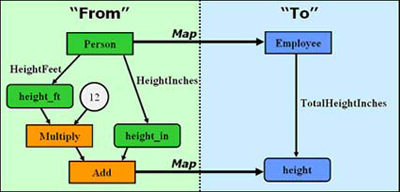
\includegraphics{Snoggle.jpg}
% \caption{Example of the graphical mapping of \emph{Snoggle} based on the Semantic Web Rule Language (SWRL)\todo[inline]{Replace by high resolution figure!}}
% \label{fig:snoggleXX}
% \end{figure}

%SNOGGLE WAS HERE


%% \begin{table*}[ht]
%%     \centering
%%     \caption{Comparison between different mapping tools}
%%     \small
%%     \begin{tabular}{@{}p{2.8cm}   p{2.1cm}   p{2.1cm}  p{2.1cm}  p{2.1cm}  p{2.1cm} @{}}
%%     \toprule
%%
%%     \textbf{Features/Tool} 	& \textbf{Ontop}	& \textbf{Revelytix Spyder}	& \textbf{Asio SBRD} 	& \textbf{Virtuoso RDF Views} 	& \textbf{D2RQ Platform}\\
%%     \midrule
%%
%%     Mapping language	& Own language	\& R2RML  	& R2RML				& Graphical 		& Own language \& R2RML 			& D2RQ-ML\\
%%     SPARQL support 		& 1.0  			& 1.1 				& × 			& 1.1 				& 1.1\\
%%     License		& Free for non-profit purposes& Free			& Commercial	 	& Free 				& Free\\
%%     Support		& Free 			& With fees 			& Commercial 		& Free 				& Free\\
%% %    DBMS Support 	& Almost all		& Almost all			& Almost all		& Virtuoso			& Almost all\\
%% % not differentiated enough
%%     \bottomrule
%%     \end{tabular}
%%     \label{tbl:toolcomparison}
%% \end{table*}
%% for non-profit purposes

\begin{table*}[ht]
    \centering
    \small
% {\textwidth}
%     \begin{tabular}{@{}p{90pt}p{60pt}p{50pt}p{80pt}p{50pt}@{}}
% \begin{tabularx}{\textwidth}{@{}XXXXXXXXXXXX@{}}
      \begin{tabularx}{\textwidth}{@{}XXXXX@{}}
      \toprule
      \textbf{Tool/Features}  & \textbf{Mapping language}   & \textbf{SPARQL Version} & \textbf{License}  & \textbf{Support}  \\
      \midrule
      Ontop~\cite{rodriguez2013evaluating}                  & Own language \& R2RML       & \centering 1.0          & Free              & Free              \\
      Revelytix Spyder        & R2RML                       & \centering 1.1          & Free              & With fees         \\
      Asio SBRD               & Graphical                   & \centering ---          & Commercial        & Commercial        \\
      Virtuoso RDF Views~\cite{virtuosoRdfViews}      & Own language \& R2RML       & \centering 1.1          & Free              & Free              \\
      D2RQ Platform~\cite{d2rserver}           & D2RQ-ML                     & \centering 1.1          & Free              & Free              \\
      Morph~\cite{priyatna2014formalisation}                   & R2RML                       & \centering 1.0          & Free              & Free              \\
      Ultrawrap~\cite{sequeda2013ultrawrap}               & R2RML                       & \centering 1.0          & Commercial        & Commercial        \\
      SparqlMap~\cite{unbehauen-jist-2012-sparqlmap}        & R2RML                       & \centering 1.0          & Free              & Commercial        \\
      Sparqlify               & R2RML \& SML                & \centering 1.0          & Free              & Free              \\
      \bottomrule
%     \end{tabular}
      \end{tabularx}
    \caption{Comparison between different mapping tools and languages.}
    \label{tbl:toolcomparison}
\end{table*}
%Sparqlify~\footnote{\url{https://github.com/AKSW/Sparqlify}}, Revelytix Spyder~\footnote{\url{http://www.revelytix.com/?q=content/spyder}}
%\tablefootnote{\url{http://www.revelytix.com/?q=content/spyder}}

%~\footnote{\url{http://www.revelytix.com/?q=content/spyder}}

%\todo{R3: Table 1 is a very general comparison. I would expect a comparison on
% the constructs and expressiveness of the different languages.}

%\section{Tabular Data to RDF Transformation}
% \section{A Formal Model for RDB2RDF Mappings}
%\vspace{-5mm}
\section{Towards a Unified Formal Model for RDB2RDF Mappings}
%\todo{first version Claus, Jens proof read}
\label{sec:model}

In this section, we outline a formal approach for mapping tabular data to RDF.
For this purpose, we first briefly summarize fundamental concepts of the RDF data model.
It should be noted, that we assume that RDF is generated by
\emph{row-wise} processing of the underlying relational data.
Both R2RML and SML build on this assumption.
Also, without loss of generality, we only consider quads rather than triples in the formalization.
The reason is, that we can view any generated triple as being labeled with the URI of the graph it belongs to.

\paragraph{Preliminaries}
\label{sec:transformation-preliminaries}
Let the RDF primitives be: $\mathcal{U}$ the set of URIs, $\mathcal{B}$ the set
of blank nodes, $\mathcal{L}$ the set of literals and $\mathcal{V}$ the set of
variables. Further:
\begin{itemize}
% \item $\mathcal{U}$ is the set of URIs
% \item $\mathcal{B}$ is the set of all blank nodes
% \item $\mathcal{L}$ is the set of all literals
% \item $\mathcal{V}$ is the set of all variables
 \item $\mathcal{T}$ is the set of all \emph{RDF term}s, defined as
  $\mathcal{U} \cup \mathcal{B} \cup \mathcal{L}$.
\end{itemize}

Furthermore, we make use of the following notions:
\begin{itemize}
  \item $\mathcal{J}$ is the joint set of RDF terms and variables, defined as $\mathcal{T} \cup \mathcal{V}$.
  \item $\mathcal{Q}$ is the set of all \emph{quads}, defined as $\mathcal{J} \times \mathcal{J} \times \mathcal{J} \times \mathcal{J}$.
  \item A \emph{quad pattern} $Q$ is a finite, possibly empty, set of quads, defined as $Q
  \subset \mathcal{Q}$
%  \todo{probably we should write "finite set" or $Q \subseteq \mathcal{Q}$?}
  \item $\mathcal{R}$ is the set of all quad patterns, thus the powerset of $\mathcal{Q}$, denoted by $\mathcal{P}(\mathcal{Q})$
  \item A \emph{quad} $q$ is defined as $q \in \mathcal{Q}$.
  \item $vars(Q)$ is the set of variables appearing in $Q$.
  \item A \emph{ground quad (pattern)} is a variable free quad (pattern).
\end{itemize}
%\footnote{For clarification: there is a small inconsistency in the terminology: A triple pattern is an element, whereas a quad pattern is a set.}

%Finally, we introduce our notion of a \emph{logical table} $L$, which we define
%as a set of partial functions that map attribute names to attribute values.
Finally, we introduce our notion of a \emph{relation instance} (short: relation) $L$, which, for convenience, we
define as a \emph{set of partial functions} that map attribute names to
attribute values.
It is noteworthy, that R2RML defines an entity referred to as \emph{logical
table}. Instances of this entity possess an
\emph{effective SQL
query}\urlfn{http://www.w3.org/TR/r2rml/\#dfn-effective-sql-query} which can be evaluated over an instance
of a database schema in order to obtain a relation.


%Finally, for ease of discussion, we introduce the function $\sigma$ that
%transforms all rows of a canonical table $C$ into a \emph{logical table} $L$,
% which is a set of corresponding partial functions from headings to data, i.e. a table
%\[
%((id, name), \{(1, Anne), (2, John) \})
%\]
%is transformed to:
%\\[
%\{ \{(id, 1), (name, Anne) \}, \{(id, 2), (name, John) \} \}
%\]

%Let $\mathcal{C}$ and $\mathcal{L}$ be the set of all canonical and logical
%tables, respectively.
%Note, that this representation is analogous to the one defined for SPARQL result sets\todo{ref to sparql spec}.
%\[
%\mathit{\sigma}: \mathcal{C} \rightarrow \mathcal{L} \newline
%\]
%\[
%\sigma(C): = \left \{ \bigcup_{1 \leq i \leq |C.H|} \left \{ (C.H_i, d_i)
% \right \} \Bigg\vert d \in C.D  \right \}
%\]

\paragraph{Generating RDF from relations}
Based on the previously introduced primitives, we are now able to formally
capture the nature of RDF mapping approaches for relational data.
%\todo{maybe
%replace tabular by relational}

A relational data to RDF (\emph{R2R}) mapping $m$ is a four-tuple $(N, P, L, f)$:
\begin{itemize}
  \item {$N$} is the \emph{name} of a view.
  \item {$P$} is a \emph{quad pattern}
%  \todo{Would it make sense to use $Q$ here as this is the latter used for quad patterns? (would need replacement further down as well)}
   which acts as the \emph{template} for the construction of triples and
   relating them to named graphs. The template is instantiated once for each row
   of the relation.
%  The use of quads enables one to map tabular data into distinct named graphs.
%  We use the notation $vars(P)$ for referring to the set of SPARQL variables
%  used in the template.
  \item {$L$} is a relation to be converted to RDF.
  \item {$f$} is a mapping with signature $L \rightarrow \left( \mathcal{V} \rightarrow \mathcal{T} \right)$:
  $f$ yields for each element of the relation $L$ a partial function that binds
  the variables of the template $P$ to RDF terms in $\mathcal{T}$.
  Note that it is not required for variables of $P$ to be bound, which enables the support NULL values in the source data.
\end{itemize}
An R2R mapping is valid, if its \emph{evaluation} yields an
\emph{RDF dataset}, as defined in the SPARQL
secification\urlfn{http://www.w3.org/TR/sparql11-query/\#rdfDataset}.
%\todo{Do we need to clarify what "conforms to" means here? Or can we just say
%that the evaluation returns a dataset (as defined in the SPARQL spec)?}

Given a quad pattern $Q \subset \mathcal{Q}$ and a partial function $a: \mathcal{V} \rightarrow \mathcal{T}$, we define the substitution operator
\[
\mathit{\rho_{[a]}}: \mathcal{R} \rightarrow \mathcal{R}
\]
$\rho_{[a]}(Q)$ yields a new ground quad pattern $Q'$ with all variables replaced in accordance with $a$. Any quads of $Q$ with unbound variables
in $a$ are omitted in $Q'$.
%\rho{a / b}(P) which replaces all variables in a quad pattern
%$
%\rho_{[a / b]} \left(R \right) := \left(
%    \rho_{[a / b]} \left( R_{D} \right),
%    \rho_{[a / b]} \left( R_{l} \right)
%\right)
%$

An evaluation of a mapping $m$ proceeds by
passing each row of $L$ as an argument to $f$,
thereby obtaining the bindings for $vars(P)$,
which are used to instantiate the template $P$
%\todo{"concrete quads" is undefined - just "quads"?}
for finally creating ground quads. Let $\mathcal{M}$ be the set of all mappings, then a function $\mathit{eval}: \mathcal{M} \rightarrow \mathcal{R}$ can be defined as:
%\[
%\mathit{eval}: \mathcal{M} \rightarrow \mathcal{R}
%\]
%\[
%eval(m) = \bigcup_{l \in m.L} \left\{ \rho_{[m.f(l)]}(m.P) \right\}
%\]

\[
eval(m) = \bigcup_{l \in L} \left\{ \rho_{[f(l)]}(P) \right\} \quad \text{ with } m = (N,P,L,f)
\]
%\todo{alternative suggestion without the dot notation}

What remains is to define a representation of the function $f$ in terms of
expressions. We refer to such a set of expressions as a \emph{variable definition}.
An analysis of the mapping languages revealed, that there is a small set
of essential operations for RDB-to-RDF mappings, for which we devised an
Extended Backus–Naur Form (EBNF) of an expression grammar as shown in
\autoref{lst:vardef} and explained as follows.

In a first step, we need to be able to construct RDF terms from the
underlying relation, hence we introduce the
\emph{rdf-term-ctor-expr}\footnote{We use \emph{ctor} as abbreviation for \emph{constructor}} production.
Note that our \texttt{plainLiteral} and \texttt{typedLiteral} functions
roughly correspond to the functions\texttt{STRDT} and \texttt{STRLANG} of the SPARQL standard,
although in SML arguments may be of types other than string, such as when mapping a column of type real to a corresponding typed literal.
Yet, in the future aliases may be introduced to SML for better alignment with existing SPARQL features.

%, and
%any variable definition that yields RDF terms would be valid for $f$.
An analysis of the mapping languages revealed, that there is a small set
of essential operations for RDB-to-RDF mappings,
namely \emph{concat}, \emph{str} and \emph{urlEncode} and
\emph{percentEncode}\footnote{\url{http://tools.ietf.org/html/rfc3986}}.
%Furthermore, for converting values from the database into IRI-safe values,
%there is also
% \emph{percentEncode}\.
These function symbols are usually used for the construction of URIs and
IRIs from values of the underlying relation: The function symbol
\emph{concat} may be used to prepend a prefix IRI to one or more ID columns.
The function symbol \emph{str} corresponds to an implicit conversion and
therefore usually does not have to be stated explicitly as it can be implied.
It is needed to preserve type consistency:
For instance, \emph{concat} is only defined for string arguments.
Therefore, \emph{concat}('http://ex.org/', 1) would yield a type error without
the prior conversion of the second argument to string.
%Another example is, that
%when creating plain l


%\todo{Can we say, e.g., that those are supported by all mapping languages
% analysed in the previous section? This part should not sound SML specific, so we might mention a reason why there are exactly those 3 (even it is obvious for you).}

Note, that although these functions could
be applied in the underlying RDBMS, support at the mapping level opens
possibilities for basic optimizations without the need to parse the involved
SQL.

%An Extended Backus–Naur Form (EBNF) of the expression grammar
%\todo{The switch from mathematical notation to EBNF might be seen as going from
% the high level model to a specific syntax already, which is a bit dangerous in this section.}
%is shown in \ref{lst:vardef}. It is noteworthy, that this grammar captures the
%essence of the constructs that R2RML introduces for the purpose of constructing
%a set of RDF terms from a row of a logical table.

\begin{lstlisting}[caption=EBNF for variable definition expressions, label=lst:vardef]
varDefinition = (var '=' rdf-term-ctor-expr)* ;

rdf-term-ctor-expr
    = bNode '(' expr ')'
    | uri '(' expr ')'
    | plainLiteral '(' expr (',' expr)? ')'
    | typedLiteral '(' expr ',' expr ')'
    ;

expr-list
    = (expr (',' expr)*)?
    ;

expr
    = var     // Denotes a reference to a column
    | str '(' expr ')'
    | concat '(' expr-list ')'
    | urlEncode '(' expr ')'
    ;
\end{lstlisting}

Example:
Assume a given relation holding the label of a product:
\[
\left\{ \left\{ (\text{id}, \text{1}), (\text{label}, \text{``Coke''}) \right\}, \ldots \right\}
\]
Assume that we aim to obtain the following assignment from variables
to RDF terms:
\[
\left\{ \left\{ (?s, \text{<http://ex.org/1>}), (?l, \text{``Coke''@en}) \right\}, \ldots
\right\}
\]

Then a definition of $f$ as
\begin{multline}
f: [\{ ?s = \text{uri}(\text{concat}(\text{'http://ex.org/'}, \text{str}(?id))), \\
      ?l = \text{plainLiteral}(?label, \text{'en'})
\}]
\end{multline}
would yield the desired output.

%\[
%f({{(id, 1)}}) = {{(?s, <http://ex.org/1>)}}
%\]

%It is noteworthy, that in practice
%\todo{Maybe say something about datatypes}
%\vspace{-5mm}
\section{SML Syntax}
\label{sec:syntax}

In this section, we give an introduction to the SML syntax.
%This is followed by a detailed formalization of the SPARQL-SQL rewriting.
%The innovation of SML's view definition syntax is to blend the concepts of
% traditional SQL \emph{Create View} statements with those of SPARQL \emph{Construct} queries.
%The mapping language is therefore composed of features that a person working on
% RDB-RDF data integration is likely to be already familiar with.
% Jens => erwähne ich jetzt später
% For this reason, we expect SML to be easier to learn and use than other mapping approaches (which define a completely new mapping language).
%imitations and future work of the language are discussed in
% \autoref{sec:conclusion}.

The left hand side of \autoref{fig:sparqlify-ml-r2rml} shows an example of SML,
whose syntactic constituents are explained as follows.

% juxtaposes the syntactic
%outline of the language with an example.

%\begin{figure}[htb]
%\centering
%\begin{tabular}{lll}
%\toprule
%\emph{Outline} & \emph{Example}  \\
%\midrule
%
%\begin{minipage}{5cm}
%\begin{scriptsize}
%\begin{verbatim}
%CREATE VIEW <name> AS
%  Construct {
%    <GraphConstructTriples>
%  }
%  WITH
%    <VariableDefinitions>
%  CONSTRAIN
%    <ConstraintDeclarations>
%  FROM
%    <LogicalTable>
%\end{verbatim}
%\end{scriptsize}
%\end{minipage}

%&


%\begin{minipage}{5cm}
%\begin{scriptsize}
%\begin{verbatim}
%CREATE VIEW hotels AS
%  CONSTRUCT {
%    ?s a ex:Hotel .
%    ?s rdfs:label ?l .
%    ?s ex:vacancy ?v .
%  }
%  WITH
%    ?s = uri(?website)
%    ?l = plainLiteral(?name, 'en')
%    ?v = typedLiteral(?vacancy,
%              xsd:boolean)
%  CONSTRAIN
%    ?s prefix "http://ex.org/"
%  FROM
%    [[SELECT website, name, vacancy
%      FROM hotels]]
%\end{verbatim}
%\end{scriptsize}
%\end{minipage}
%
%\end{tabular}
%\caption{SML view definition syntax.}
%\label{fig:sparqlify-ml}
%\end{figure}



Recall that in the previous~\autoref{sec:transformation-preliminaries} we
formally defined an R2R view as a four-tuple $(N, P, L, f)$.
The core syntax of an SML view definition comprises four parts that correspond
directly to the formal definition. Additionally, SML features
an optional \emph{constraint} component for improving query performance.
%a \emph{constraint} component, that turned out to be useful in pratice.
An SML view definition is composed of the following parts:
\begin{itemize}
  \item The \emph{name} of the view. This corresponds to an element of the
  set $N$.

  \item A \emph{construct} clause, which consists of triple patterns
  which can be optionally associated with a specific named graph by
  surrounding
  them with \texttt{GRAPH }$G${ \{ \ldots \}}, where $G$ can be a variable name
  or an IRI.
  %The syntax is therefore a slight extension of the \emph{ConstructTemplate}
  % production rule\footnote{\url{http://w3.org/TR/rdf-sparql-query/\#sparqlGrammar}} of SPARQL.
  Hence, the syntax is equivalent to the \emph{quads} production rule of the
  SPARQL 1.1 standard\footnote{\url{http://www.w3.org/TR/sparql11-query/\#rQuads}}.
  This corresponds to an element of $P$.

  \item A \emph{FROM} clause, where a reference to a \emph{logical table} can be specified.
  As in R2RML, this can be either an SQL SELECT statement, the name of a
  physical table or the name of a view.
  The former needs to be escaped in triple double-quotes, i.e. \texttt{"""SELECT \ldots"""}.
  The execution of a logical table's effective SQL query over an SQL connection
  yields a result set which formally corresponds to $L$.

  \item The \emph{variable definition clause} acts as the bridge between the RDF
  and SQL data models, and is used to specify the creation of RDF terms from
  rows of the relation.
  It consists of a set of \emph{variable definition statements} of the
  form \emph{?var = rdf-term-ctor($expr_0$, \ldots, $expr_n$)}, and should
  at least support the grammar defined in \ref{lst:vardef}.

%
%  \begin{itemize}
%    \item $\mathit{termctor}$ refers to the RDF term constructor, which can be
    % \texttt{bNode}, \texttt{uri}, \texttt{plainLiteral}, or \texttt{typedLiteral}. %It is discussed in more details in\todo{reference - I want to say something about its datatypes}.
%    \item $expr_i$ refers to expressions over sets of SQL column references of
    % the logical table and constants.
%			Syntactically, the currently supported operators in variable definition
            % expressions are:
%			\texttt{concat}, \texttt{urlEncode} and \te.%Note that our
            %formalization arbitrary SQL expressions are allowed.
%    \item $var$ is a SPARQL variable being defined, which should be referenced
    % from the construct clause.
            %Note that these expressions are treated specially by the Sparqlify engine's optimizer.
            %Sparqlify does not try to understand the SQL, for this reason expressions
            %Note that expressions stated in the projections of SQL queries are not subject to query optimization by Sparqlify.
%  \end{itemize}

  \item Finally, there is a \emph{CONSTRAINT} clause for specifying
  contstraints about variables on the RDF level. As such, it has no direct
  influence on the virtual RDF relation, but rather on query performance.
  The example in \autoref{fig:sparqlify-ml-r2rml} shows, that
  solely based on the definition of $?s = uri(?website)$ we have no information
  about the set of URIs being created. Specifying such a type of constraints
  enables SPARQL-to-SQL rewriters, for instance, to prune joins whose join
  condition equates variables with disjoint sets of prefixes. Syntactically, up
  to now only stating prefix constraints is supported.
   %can be explicitely
  %specified.
  %Internally, however, constraints are used to restrict predicates to URIs or
  % subjects to blank nodes and URIs.
\end{itemize}

%It is noteworthy that the `variables' used as arguments of the term
%constructors are column references to the relation and as such carry a SQL
%datatype.
%This means that RDB2RDF mappings need to be datatype aware.



%\begin{definition}[Correctness and Completeness of Rewrites]
%RDF-Relation = materialize(Views, Database)

%DumpQueryResultSet = Execute(RDF-Relation, SparqlQuery)

%Rewrite(SparqlQuery, Views) returns (SqlQuery, Map)
%ViewQueryResultSet = Map(Execute(Database, SqlQuery))

%Correct: ViewQueryResultSet subset DumpQueryResultSet
%Complete: ViewQueryResultSet superset DumpQueryResultSet


%TODO Place datatypes into the view definition? I guess this makes most sense,
%because then we do not have to carry the database around.

%TODO How to show that we are preserving this for most of the time?
%\end{definition}



%\vspace{-5mm}
\section{Comparison of SML with R2RML}
\label{sec:sml-vs-r2rml}
%--\todo{R3: section 5 is titled "Comparison of SML with R2RML" whereas the contribution of the paper is supposed to be  the converters of the languages - both ways. If this is the case, then the section title should be changed and the mappings of SML to R2RML and vice versa should be defined or at least a Table of the correspondence between the constructors of both languages should be presented, it is only presented for term constructors to term maps.}
In this section, we summarize essential features of R2RML and explain how
they relate to those of SML.
R2RML mappings are expressed as RDF graphs for which R2RML by convention uses
Turtle serialization. The fundamental class is \texttt{rr:TriplesMap}, whose
instances are specifications of the triples to generate from an underlying
logical table.
As such, an instance of a TriplesMap corresponds to an SML view definition.
In the following, we explain the most important attributes that TriplesMaps
may have, and compare them to SML.
\autoref{fig:sparqlify-ml-r2rml} shows a side-by-side
comparison of the mapping languages for a specific example.
Both syntactic formats can be converted to each other.

\begin{figure*}[t]
\centering
\begin{tabular}{@{}ll@{}}
\toprule
\emph{SML} & \emph{R2RML}  \\
\midrule
  \begin{minipage}{0.38\linewidth}
    \begin{scriptsize}
\begin{verbatim}
Prefix rdfs: <http://www.w3.org/2000/01/rdf-schema#>
Prefix xsd: <http://www.w3.org/2001/XMLSchema#>
Prefix ex: <http://ex.org/>

Create View hotels As
  Construct {
    ?s a ex:Hotel ;
      rdfs:label ?l ;
      ex:vacancy ?v
  }
  With
    ?s = uri(?website)
    ?l = plainLiteral(?name,'en')
    ?v = typedLiteral(?vacancy,
              xsd:boolean)
  Constrain
    ?s prefix "http://ex.org/"
  From
    """SELECT website, name,
      vacancy FROM hotels"""
\end{verbatim}
    \end{scriptsize}
  \end{minipage}
  &
  \begin{minipage}{0.60\linewidth}
\begin{scriptsize}
\begin{verbatim}
@prefix rdfs: <http://www.w3.org/2000/01/rdf-schema#> .
@prefix xsd: <http://www.w3.org/2001/XMLSchema#> .
@prefix ex: <http://ex.org/> .

<HotelTriplesMap>
  rr:logicalTable [ rr:sqlQuery
  """SELECT website, name,
  vacancy  FROM hotels""" ];

  rr:subjectMap [
    rr:column "website";
    rr:class ex:Hotel
  ];
  rr:predicateObjectMap [
    rr:predicate rdfs:label;
    rr:objectMap
      [ rr:column "name";
        rr:language "en"];
  ];
  rr:predicateObjectMap [
    rr:predicate ex:vacancy;
    rr:objectMap
      [ rr:column "vacancy";
        rr:datatype
          xsd:boolean ];
  ].
  \end{verbatim}
\end{scriptsize}

\end{minipage}
\\\bottomrule
\end{tabular}
%\vspace{-5pt}
\caption{A simple view in SML and R2RML.}
\label{fig:sparqlify-ml-r2rml}
\end{figure*}%\todo{The rdf:type predicateObjectMap is missing in the `A simple view in SML and R2RML' figure. Maybe use ldots to show that it is left out intentionally}

%The following paragraphs
%we base our discussion on the paragraphs as they
%appear in the R2RML standard.

% is an RDF vocabulary for expressing
%RDB2RDF mappings
%, originally inspired by the D2RQ mapping vocabulary.
%R2RML and SML are both very recent and
%independent efforts whereas the latter has since then evolved into a W3C
% Proposed Recommendation\footnote{\url{http://www.w3.org/TR/r2rml/}}.
%The core concepts of R2RML have semantically equivalent counterparts in
%SML and vice versa.

% However, users can benefit from SML for
%two reasons:
%\begin{itemize}
%  \item We expect SML to be easier to learn and use for typical users than other mapping approaches, including R2RML, since it composes SPARQL and SQL constructs with few additional constructs.
%  \item For typical RDB2RDF mapping authors, we expect SML to be easier to
  % learn and use than other mapping approaches, including R2RML, since it composes SPARQL and SQL constructs with few additional syntactical elements.
%  \item The SML syntax is more compact due to less syntactic noise created by
  % using an XML based format.
%  \item The syntax and the corresponding formal model are conceptually very close.
%\end{itemize}

%A potential further advantage is that the syntax and the underlying formal
% model are conceptually closer in SML than in R2RML.
%
%RDF generation is performed in both cases by applying on logical tables
% row-wise mapping instructions.
% their RDF terms are constructed in R2RML and outline their corresponding SML expressions.

%\vspace{-5mm}
\paragraph{Defining Logical Tables}
R2RML defines the predicate \texttt{rr:logicalTable} to relate a TriplesMap to a
logical table. The object of this predicate must be a resource that is further
described using \texttt{rr:tableName} or \texttt{rr:sqlQuery}.
A TriplesMap must have exactly one logical table.
In SML, the \emph{FROM} clause serves the same purpose.
\autoref{tbl:from-clause} compares how to state a logical table in
R2RML and SML.
%Note that in SML it is valid to omit the FORM and WITH clause, if the template
%only contains concrete quads. A common use case is specifying parts of the
%vocabulary, such as domain and range.

%Note that in SML
%it is valid to omit the FROM and WITH clause, if the template only holds
%concrete quads. Technically, it is equivalent to using [[SELECT 1]]

\begin{table}[!h]
\centering
\begin{scriptsize}
\begin{tabular}{ll}
\toprule
rr:tableName "person"       & \ldots From person \\
rr:tableName "SCOTT.DEPT"   & \ldots From "SCOTT.DEPT" \\
rr:sqlQuery """SELECT \ldots""" & \ldots From """SELECT \ldots""" \\
%\midrule
\bottomrule
\end{tabular}
\end{scriptsize}
\caption{Comparison of attributes of rr:logicalTable with SML's FROM clause.}
\label{tbl:from-clause}
\end{table}

% omitted due to space

%A minor difference is that R2RML additionally supports stating the dialect of
%an SQL query using the \texttt{rr:sqlVersion} property, which at present, has no counterpart in SML.
%This flag could be used to hint a mapping processors to pick a specific SQL parser in
%order to obtain the query's corresponding algebraic representation and potentially apply optimizations. \todo{If we do not have space, I would omit this point as it seems that this could also be added to SML without much effort.}

%\todo{We could argue that this should be set on DB level rather than view
% level.}

%We point out the most important similarities: % describe here how quads and

%\vspace{-5mm}
\paragraph{Creating RDF terms from logical tables}
Both SML and R2RML allow to express how to create RDF terms from the
rows of the underlying logical table. In SML, the term constructor
expressions
%\todo{It would probably be good to introduce the abbreviation "TCE" in the previous section, which already introduces the syntax?}
of the WITH clause serve this purpose, whereas R2RML introduces the notion of \emph{TermMaps}.
SML uses an expression syntax to specify the RDF term creation, which corresponds to
using a combination of the properties \texttt{rr:template},
\texttt{rr:termType} and \texttt{rr:datatype} in R2RML.
The template syntax for values of \texttt{rr:template} corresponds to
the SML expression symbols \emph{concat} and \emph{urlEncode}.
%\todo{urldecode was mentioned in the previous section as well}
\autoref{tbl:termconst2termmap} shows examples of RDF term construction in
both mapping languages. The function \emph{asTemplate(expr)} is assumed to
yield the R2RML template for a given SML expression.
Note that SML is slightly more expressive in this regard, as it
allows e.g.~nested urlEncodings.
%However, the practical use may be limited.

\begin{table}
  {\scriptsize
  \begin{tabular}{@{}p{0.43\linewidth}p{0.55\linewidth}@{}}

    \toprule
    SML RDF term constructor                        & R2RML term map \\
    \midrule
    \texttt{bNode(?COL)}                        & \texttt{\ldots\ [ rr:column "COL" ; } \\
                                                    & \hspace{22pt}\texttt{rr:termType rr:blankNode ]}\\
    \midrule
    \texttt{bNode(\emph{expr})}           & \texttt{\ldots\ [ rr:template "\emph{asTemplate(expr)}" ; } \\
                                                    & \hspace{22pt}\texttt{rr:termType rr:blankNode ]}\\
    \midrule
    \texttt{uri(\emph{expr})}                 & \texttt{\ldots\ [ rr:\emph{(constant|column|template)} "\emph{asTemplate(expr)}";} \\
                                                    & \hspace{22pt}\texttt{rr:termType rr:IRI ]} \\
    \midrule
    \texttt{plainLiteral(?COL)}                     & \texttt{\ldots\ [ rr:column "COL" ] } \\
    \midrule
    \texttt{plainLiteral(\emph{expr})}        & \texttt{\ldots\ [ rr:template "\emph{asTemplate(expr)}" ] } \\
    \midrule
    \texttt{typedLiteral(?COL, \emph{xsd:int})}& \texttt{\ldots\ [ rr:column "COL" ; } \\
                                                    & \hspace{22pt}\texttt{rr:datatype \emph{xsd:int} ]}\\
    \midrule
    \texttt{typedLiteral(\emph{expression}, \emph{xsd:int})}
                                                    & \texttt{\ldots\ [ rr:template "\emph{asTemplate(expr)}" ;} \\
                                                    & \hspace{22pt}\texttt{rr:datatype \emph{xsd:int} ]} \\
    \bottomrule
  \end{tabular}
  }
  \caption{Transformation of SML term constructors to R2RML term maps}
  \label{tbl:termconst2termmap}
\end{table}


\paragraph{Forming Quads from RDF Terms}
Once there exists a specification of how to create RDF terms from the rows of a
logical table, these RDF terms need to be grouped to form quads.
In SML, this is done using the CONSTRUCT clause, which re-uses the quads
production rule of the SPARQL 1.1 standard.
Hence, anyone familiar with SPARQL should already be familiar with SML in this regard.

In R2RML, the TriplesMap serves this purpose, however its specification is more
verbose:
For relating a TriplesMap to TermMaps for the subject, predicate, object and
graph components, there exist the general properties \texttt{rr:subjectMap},
\texttt{rr:predicateMap}, \texttt{rr:objectMap} and \texttt{rr:graphMap},
respectively.
Note that for each of these properties there exists a syntactic
shortcut without the \emph{Map} in the name, that can be used for constants.

%Note that R2RML features several syntactic short cuts, however the following

% in cases where the
%value is a constant, rather than being created from the logical table.

These properties are used to form the following structure:
Every TriplesMap carries exactly one specification for its subjects, and zero or
more specifications for the pairs or predicates and objects.
Subjects are specified by relating the TriplesMap to a TermMap
using \texttt{rr:subjectMap}.
A SubjectMap may carry zero or more attributes of \emph{rr:graphMap} and \emph{rr:class}.
The former specifies in which graphs the generated triples reside.
The latter is a syntactic shortcut for \emph{rdf:type}'ing the subjects with
given IRIs.
Zero or more \emph{rr:predicateObjectMap} attributes denote the
predicate-object-pairs to associate with each subject.
Thereby, each PredicateObjectMap carries the attributes \emph{rr:objectMap} and
\emph{graphMap}, which again are TermMaps.


%Also,
%rr:template "http://ex.org/dept/{dept_id}"


% for expressing which quads to create, however, this approach is
%more verbose:

%First, a resource of \texttt{rr:TriplesMap} has to be created.

%\texttt{rr:predicateObjectMap}
%This resource then acts as a container for the descriptions about how to create
%a set of quads.
%The predicate \texttt{rr:subjectMap} is used to associate a TriplesMap to

% set of triples having the same subject.
% This resource then needs to be described using \texttt{rr:subjectMap}, which


%The subject to be created is expressed in a \emph{term map} which is usually
% defined via two additional statements.
%Further definitions of how the predicates and objects are generated, are
% attached to a \texttt{rr:predicateObjectMap} resource, which is part of the triples map.
%The actual predicate and object definitions are again term maps.
%Using the shortcut for constant expressions, a triple generation pattern with a
% constant predicate will then require at least six RDF statements on three different blank nodes.


%resources of type
%R2RML' triple maps are essentially
%
%
%\todo{Citation}
%The RDF triples generated from one row in the logical table all share the same subject.

%R2RML \emph{term maps} are the actual construction plan for the triple nodes to
% create.
%In R2RML three different cases are covered by term maps.
%An RDF node can be constant, can be generated using the value of a column of
% the underlying relational table, or it can be built using a certain template string, where the column value is embedded.
%In SML \emph{RDF term constructors} serve the same functionality, but in a more
% generic way.
%Here, no distinction is made between the usage of the column value alone or
% template expressions, since the term constructor input can be an arbitrary expression, be it the placeholder of a column alone or the result of the concatenation with further string expressions or column references.
%Besides this, SML needs no extra term type definition statements, as is the
% case in R2RML, since the term constructor already determines, what kind of RDF node to generate.

%\vspace{-5mm}
\paragraph{Foreign Key Relations among Logical Tables}
%\todo{We can differ between two use cases: 1. Expression of joins 2.
% Referencing variables of other views.}

%\todo{can we remove "limited" - if we get a reviewer not knowing the details,
%they could see this as negative}
R2RML offers a model for the expression of joins.
This model is primarily intended for
%simpliying
the generation of IRIs
that require a join of tables between one or more foreign key constraints to hold.
The R2RML vocabulary distinguishes the roles of the \emph{parent} and \emph{child} table,
where the child references the parent on a certain \emph{join condition}.
%This modeling serves two purposes: On the one hand, it is a syntactic shortcut,
%as the child TriplesMap can refer to the TermMap of the parent
%TriplesMap's subject, rather having to duplicate this TermMap.
%On the other hand,

%There is no
SML offers a limited SQL syntax for this purpose, which is shown and compared to
R2RML in~\autoref{fig:sml-r2rml-refobj}. Note, that in contrast to using SML's
triple double-quotes syntax for stating SQL queries, this
syntax allows the SML processor to understand the SQL natively (i.e.
without requiring an full SQL parser) and thus consider it for optimizations
such as self join elimination.

\begin{figure*}[tb]
\centering
\begin{tabular}{@{}ll@{}}
\toprule
\emph{SML} & \emph{R2RML}  \\
\midrule

  \begin{minipage}{0.38\linewidth}
    \begin{scriptsize}
\begin{verbatim}
Prefix ex: <http://ex.org/>

Create View departments As
  Construct {
    ?d a ex:Department
  }
  With
    ?d = uri(ex:dept, ?name)
  From
    departments

Create View employees As
  Construct {
    ?e a ex:Employee ;
      ex:worksIn ?d
  }
  With
    ?e = uri(ex:emp, ?e.id)
    ?d = uri(ex:dept, ?d.name)
  From
    employees e Join departments d
      On (d.id = e.dept_id)
\end{verbatim}
    \end{scriptsize}
  \end{minipage}

&
  \begin{minipage}{0.60\linewidth}
    \begin{scriptsize}
\begin{verbatim}
@prefix ex: <http://ex.org/> .

<#Departments>
  rr:logicalTable [ rr:tableName "departments" ];

  rr:subjectMap [
      rr:template "http://ex.org/dept/{id}" ];
      rr:class ex:Department
  .

<#Employees>
  rr:logicalTable [ rr:tableName "employees" ];

  rr:subjectMap [
      rr:template "http://ex.org/emp/{id}" ;
      rr:class ex:Employee ];

  rr:predicateObjectMap [
    rr:predicate ex:worksIn;
    rr:objectMap [
      rr:parentTriplesMap <#Departments>;
      rr:joinCondition [
        rr:child "dept_id";
        rr:parent "id";
      ];
    ];
  ].
\end{verbatim}
    \end{scriptsize}
  \end{minipage}
\\
\bottomrule
\end{tabular}
%\vspace{-5pt}
\caption{A view in SML and R2RML with a referencing object map.}
\label{fig:sml-r2rml-refobj}
\end{figure*}

%\vspace{-15pt}

%\begin{table}
%\centering
%\begin{tabular}{lp{2em}l}
%\toprule
%rr:tableName "person" &&  \ldots From parent a, child b WHERE b.parent\_id =
% a.id \\
%\midrule
%\bottomrule
%\end{tabular}
%\end{table}
%Note that expressing a join with this syntaxt is different from using the SQL query string syntax

% \todo{I don't understand
% this part. Whether you put brackets around or not, the SML processor can understand the query, right?}

%\vspace{-5mm}
\paragraph{Assigning Triples to Named Graphs}
To assign triples to be generated to a certain named graph, again term maps are utilized.
Accordingly, an additional term map inside a subject or predicate map is defined, which is called \emph{graph map}.
These nested term map expressions introduce further complexity to the actual triples map.

%\begin{table}
%\centering
%\begin{tabular}{lp{2em}l}
%\toprule
%rr:tableName "person"        &&  Create View \ldots From person \\
%rr:sqlQuery "SELECT \ldots"  &&  Create View \ldots From [[SELECT \ldots]] \\
%\midrule
%
%\bottomrule
%\end{tabular}
%\end{table}

%begin{description}
% \item [RDF Term Generation]
%R2RML defines the \emph{term map} as a function that generates RDF terms from rows.
%These term maps can either be constant, column based or derived from a column
%using a template. Term maps are therefore conceptually equivalent to
%SML's term constructors.


% \item [Quad Generation]
%\paragraph{Quad Generation:}
% For generating quads, R2RML utilizes \emph{triple map}s and \emph{graph map}s.
% Triple maps align \emph{term map}s to form triples, whereas graph maps relate
% these triples to a named graph. As such, this is exactly what SML
% expresses using a conventional SPARQL CONSTRUCT template.
% \item [References] R2RML allows relating \emph{triple maps} by directly
% referencing triple maps.
% Sparqlify implicitly creates relations by utilizing term constructors that
 % create the same terms.
%\end{description}


%\vspace{-5mm}
\section{Converting SML to R2RML}
\label{sec:sml2r2rml}
%%--\todo{R4: There is no discussion how R2RML can be converted to SML}
%We provide a tool for the
%automatic conversion
%of SML \footnote{\url{http://purl.org/org/aksw-research/resources/sml}}.
%\todo{Can we put this under an sml.aksw.org URL as well to not be Sparqlify specific?}.
%To be able to translate SML view definitions into R2RML mappings, we provide a tool for an automatic conversion\footnote{\url{http://sparqlify.org/wiki/Project_R2RML_Export}}% \todo{Can we put this under an sml.aksw.org URL as well to not be Sparqlify specific?}.
In this section, we briefly outline the approach for the conversion of SML to
R2RML.
%Given an SML view, the translation proceeds as follows:
%Possible prefix definitions are not shown there for brevity but their translation is simple:
The process of converting prefix definitions is straightforward since the only
difference is that SML uses the \texttt{Prefix} keyword, whereas in R2RML turtle notation \texttt{@prefix} is used.
%a given SML prefix definition, e.g. `\texttt{\footnotesize Prefix spy: <http://aksw.org/sparqlify/>}' will be converted to `\texttt{\footnotesize@prefix spy: <http://aksw.org/sparqlify/>.}' .
The name of an SML view definition serves as a base for crafting the IRIs for
naming triples maps.
However, it has to be taken into account that one SML view definition can correspond to many R2RML triples maps. %e.g. \texttt{\footnotesize hotels}, defined via `\texttt{\footnotesize Create View hotels AS}'
The definition of a logical tables as table names, view names or queries have
direct counterparts in R2RML, namely \texttt{rr:tableName} and
\texttt{rr:sqlQuery}.

The SML \texttt{CONSTRAINT} clause has no equivalent in R2RML and
is thus omitted in the conversion. Note that constraints only act as hints that
may be considered for improving performance.%, but they have no influence on the generation of quads.


%So there could possibly be the need to pre- or postfix the view definition name, e.g. with running numbers for the different triples maps.

%In case of a relational table, e.g. \texttt{\footnotesize persons}, one would extract the R2RML logical table definition `\texttt{\footnotesize rr:logicalTable [ rr:tableName "persons" ]}'.
%In case of a relational table, the R2RML logical table definition with the
%corresponding \texttt{rr:tableName} expression will be extracted.
%If an SQL expression is given instead, e.g. `\texttt{\footnotesize [[SELECT website FROM hotels]]}', the R2RML translation would be `\texttt{\footnotesize rr:logicalTable [ rr:sqlQuery "SELECT website FROM hotels" ]}'.
%If an SQL expression is given instead, the \texttt{rr:sqlQuery} property is
% used instead.
%The SML statements expressing a table join, as in \texttt{\footnotesize FROM dept d, employee e WHERE d.id = e.dept\_id } would be converted using

%the translated R2RML triples maps and can so be ignored during conversion.

The \emph{Construct} and \emph{With} sections of an SML do not directly
translate to R2RML.
In general, a new triples map
%carrying a
%\texttt{rr:graphMap}, \texttt{rr:subjectMap}, \texttt{rr:predicateMap} and
%\texttt{rr:objectMap}
can be created for each quad of the \emph{Construct} section.
However, if an SML view defines multiple quads with the same
variable in the subject position, multiple instances of
\emph{rr:predicate\-ObjectMap} can be created on the same triples map.

%In general, the correspondences of \autoref{tbl:termconst2termmap} apply,
%however in inverse direction.
%Variable-free expressions can be directly converted to
%term maps with an \texttt{rr:constant} value.
%In the case of expressions with variables, the definitions of the \texttt{With}
%section have to be taken into account.

%relevant outermost term constructors in combination with possible constructor
% inputs and the resulting R2RML term maps.
Regarding the constructor arguments, one has to differentiate between an atomic
value and a compound expression.
An atomic value can either be a column reference, resulting in an \emph{rr:column} term map or a constant expression requiring \emph{rr:constant}.
In all other cases, a more complex expression is assumed, resulting in an
\emph{rr:template}.
Such an expression has to be evaluated from the innermost to the outermost term constructor which leads to the evaluated expression shown in \autoref{tbl:termconst2termmap}.

%This can be seen in the example in \autoref{fig:sparqlify-ml-r2rml}.

An even more complex R2RML mapping has to be created if an SML variable already used in subject position is also referred to in the object position of another \texttt{Construct} statement.
In this case a referencing object map has to be used in R2RML.
An example and the corresponding triples maps are shown in \autoref{fig:sml-r2rml-refobj}.
%
There, the definition of the \texttt{rr:joinCondition} can be omitted since both triples maps refer to the same logical table.
Note, that R2RML only provides a language expression to declare referencing
objects and not for e.g. predicates and graphs.
%There are no means to express a referencing predicate.
A conversion from R2RML to SML proceeds in a similar fashion as described in
this section, however details are omitted for brevity.
%convert for SML to R2RML exists, but

%As a consequence SML \texttt{With} statements like \texttt{?p a rdf:Property. ?s ?p ?o.} cannot be translated into R2RML showing that SML is more expressive in this case.

%If the SML join notation is used to refer to foreign key relations one cannot translate this into an R2RML join without knowing the underlying database schema.\todo{PW: AFAIK. I did not get that much information about SML joins so far, so if these assumptions are wrong, please give feedback.}\
%So the generic approach here would be to translate this expression into an \texttt{rr:sqlQuery} an use this as logical table.


%\begin{table}
%  {\scriptsize
%  \begin{tabular}{p{0.49\linewidth}p{0.49\linewidth}}
%    \toprule
%    SML term constructor                            & R2RML term map \\
%    \midrule
%    \texttt{blankNode(?COL)}                        & \texttt{\ldots\ [ rr:column "COL" ; } \\
%                                                    & \hspace{28pt}\texttt{rr:termType rr:blankNode ]}\\
%    \midrule
%    \texttt{blankNode(\ldots(\ \ldots\ )\ldots)}    & \texttt{\ldots\ [ rr:template "\ldots" ; } \\
%                                                    & \hspace{28pt}\texttt{rr:termType rr:blankNode ]}\\
%    \midrule
%    \texttt{uri(\ldots)}                            & \texttt{\ldots\ [ \hspace{14pt}\ldots\hspace{14pt} ;} \\
%                                                    & \hspace{28pt}\texttt{rr:termType rr:IRI ]} \\
%    \midrule
%    \texttt{plainLiteral(?COL)}                     & \texttt{\ldots\ [ rr:column "COL" ] } \\
%    \midrule
%    \texttt{plainLiteral(\ldots(\ \ldots\ )\ldots)} & \texttt{\ldots\ [ rr:template "\ldots" ] } \\
%    \midrule
%    \texttt{typedLiteral(?COL, xsd:sometype)}       & \texttt{\ldots\ [ rr:column "COL" ; } \\
%                                                    & \hspace{28pt}\texttt{rr:datatype xsd:sometype\ ]}\\
%    \midrule
%    \texttt{typedLiteral(\ldots(\ \ldots\ )\ldots, xsd:sometype)}
%                                                    & \texttt{\ldots\ [ rr:template "\ldots" ;} \\
%                                                    & \hspace{28pt}\texttt{rr:datatype xsd:sometype ]} \\
%    \bottomrule
%  \end{tabular}
%  }
%  \caption{Transformation of SML term constructors to R2RML term maps}
%  \label{termconst2termmap}
%\end{table}


% noch nicht fertig
%\section{Usability Study}[Jörg,Claus]
% Experiment SW Praktikum

% \section{Related Work}
% \label{sec:related}

% check whether we need the section

%\todo[inline]{Do we have any statistics on how much less symbols SML mappings
% require compared to R2RML?}

%\todo[inline]{What about the other direction? We could just mention that a
% convert for SML to R2RML exists, but details are omitted for brevity.}

%%--\todo{I do not have experience on comparing Domain Specific Languages. But
% I'm sure there is literature on this area. For example, a quick search yielded:
%Marjan Mernik, Jan Heering, and Anthony M. Sloane. 2005. When and how to
% develop domain-specific languages. ACM Comput. Surv. 37, 4 (December 2005), 316-344.
%This type of work seems very relevant. None of this related work is taken in
% account.}


%\vspace{-5mm}
\section{Evaluation}
\label{sec:eval}

\begin{table*}[!t]
\begin{subfigure}[c]{0.45\textwidth}
\begin{tabular}{@{}lr@{}}
 criterion & value \\\toprule
Relevance : & 4.15 \\
Familiarity TTL :  & 4.11 \\
Familiarity SPARQL:  & 4.30 \\
Familiarity SQL :  & 4.33 \\
Familiarity R2RML :  & 3 \\
Familiarity SML :  & 1.74 \\
\end{tabular}
\end{subfigure}
\begin{subfigure}[c]{0.45\textwidth}
\begin{tabular}{@{}lr@{}}
 criterion & value \\\toprule
Average Understandability R2RML : & 3.85 \\
Average Understandability SML : & 3.88 \\
Average Readability R2RML : & 3.26 \\
Average Readability SML : & 3.72 \\
Average Considering SML  : & 3.59 \\
Average Preference R2RML - SML: &  3.26
\end{tabular}
\end{subfigure}
\caption{Averaged results of survey questions (1 = lowest rating, 5 = highest rating).}
\label{tab:eval_overview}
\end{table*}

\begin{figure*}[!t]
 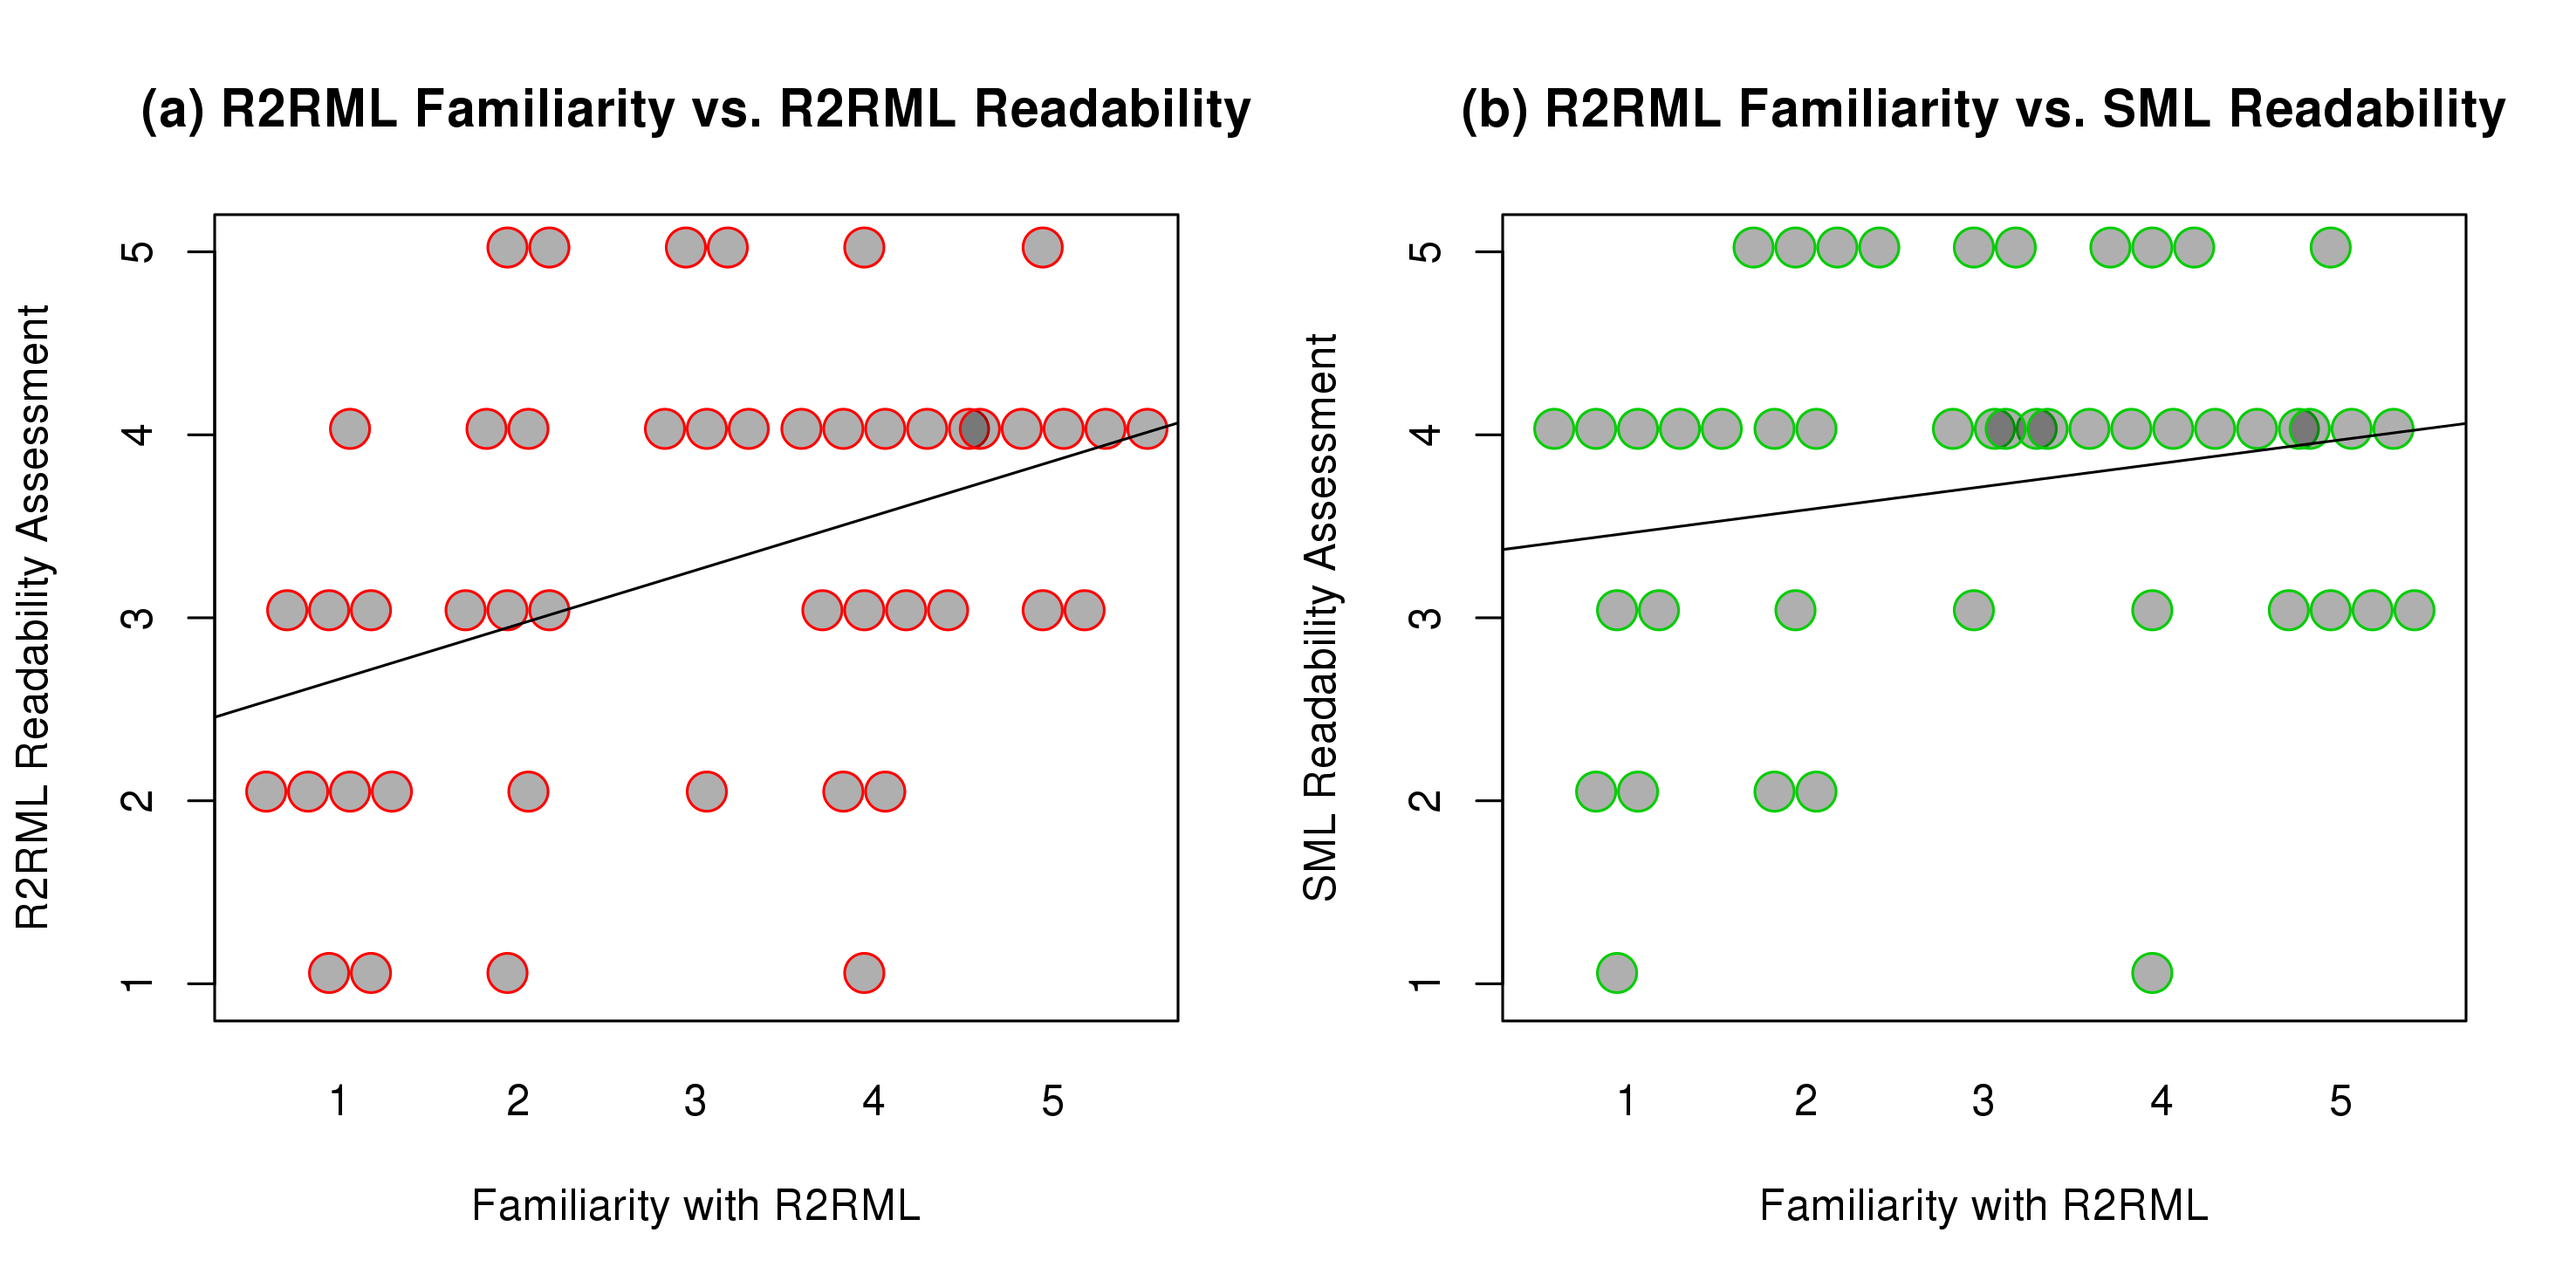
\includegraphics[width=\textwidth]{pics/fam_vs_read}
%\vspace{-15pt}
 \caption{The plot shows the R2RML familiarity plotted against the readability assessment of R2RML and SML. Overall, SML was judged to be significantly more readable although this effect is reduced for participants already familiar with R2RML.}
 \label{fig:fam_vs_read}
\end{figure*}


\begin{figure*}[!t]
%\begin{subfigure}[c]{0.5\textwidth}
%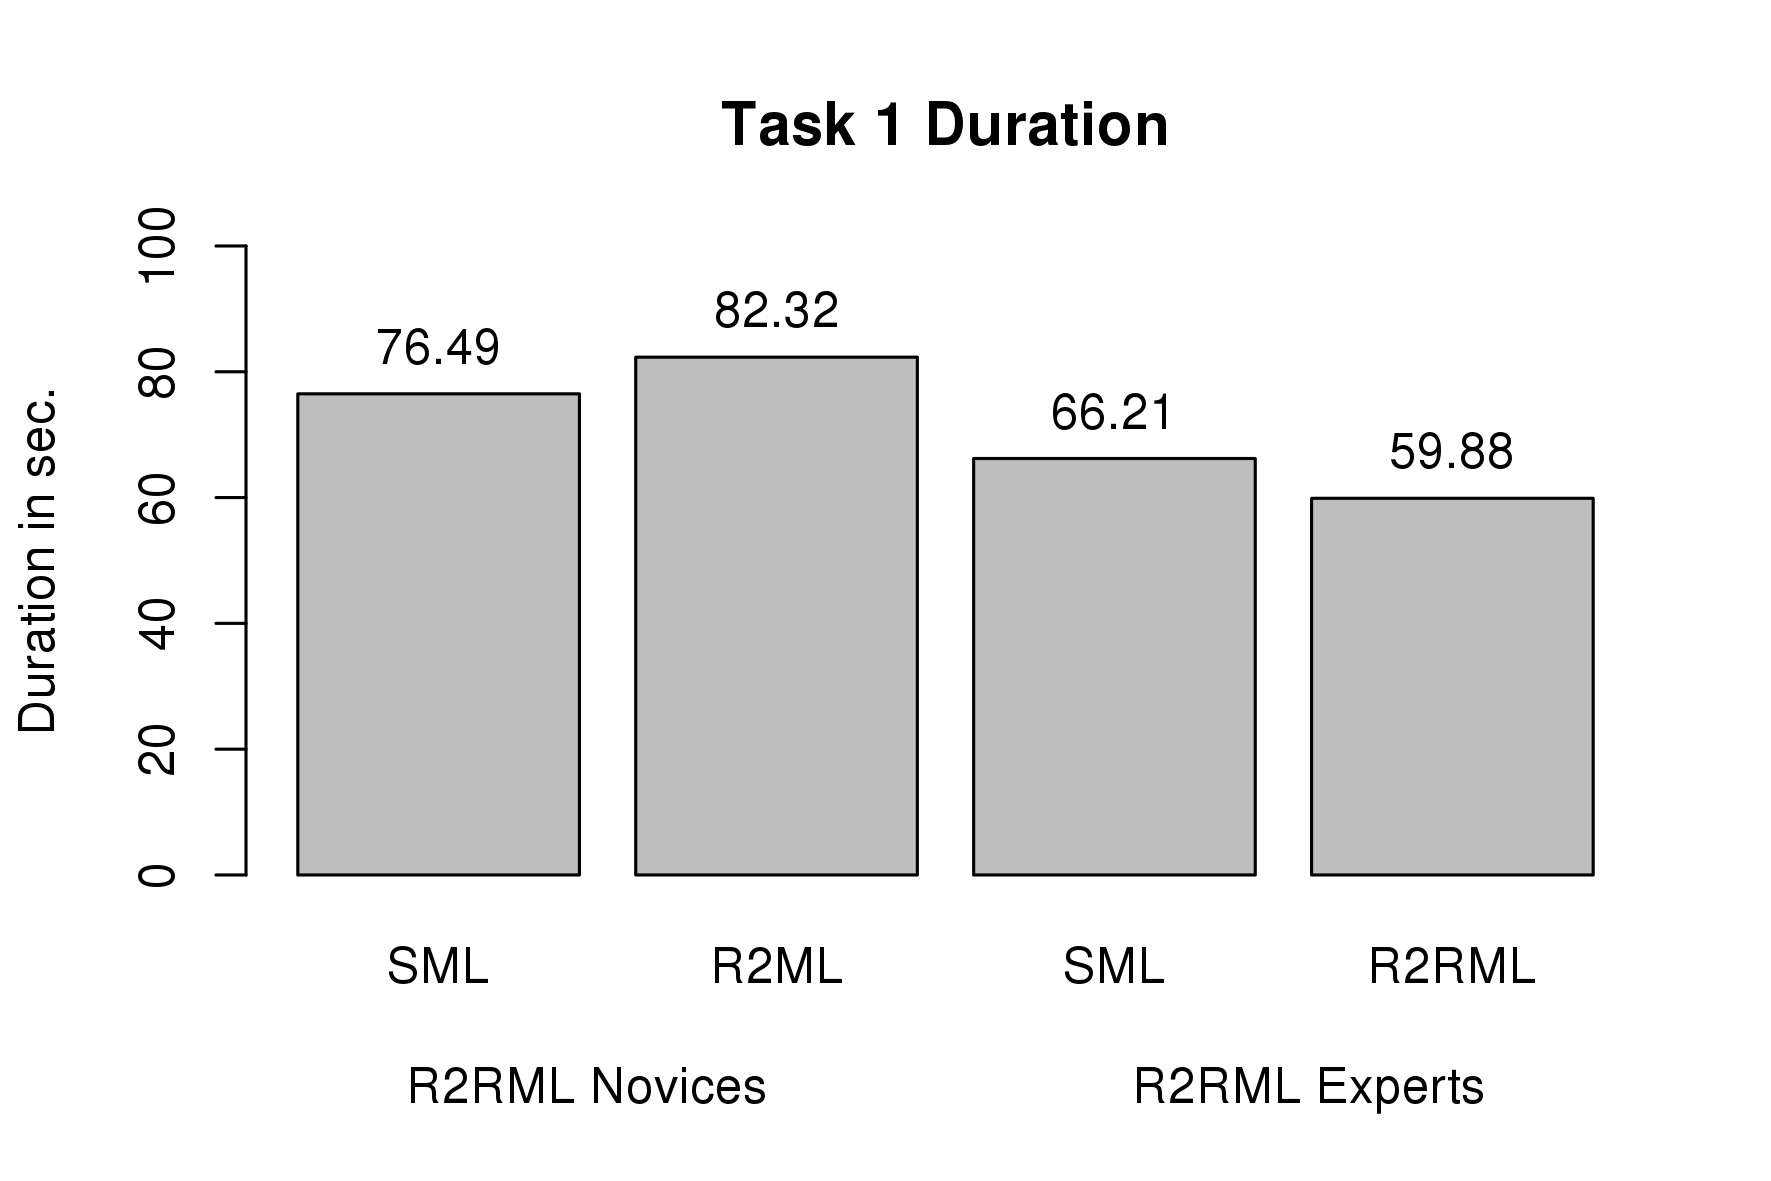
\includegraphics[width=0.99\textwidth]{pics/task1_duration}
%\subcaption{xy}
%\end{subfigure}%
%\begin{subfigure}[c]{0.5\textwidth}
%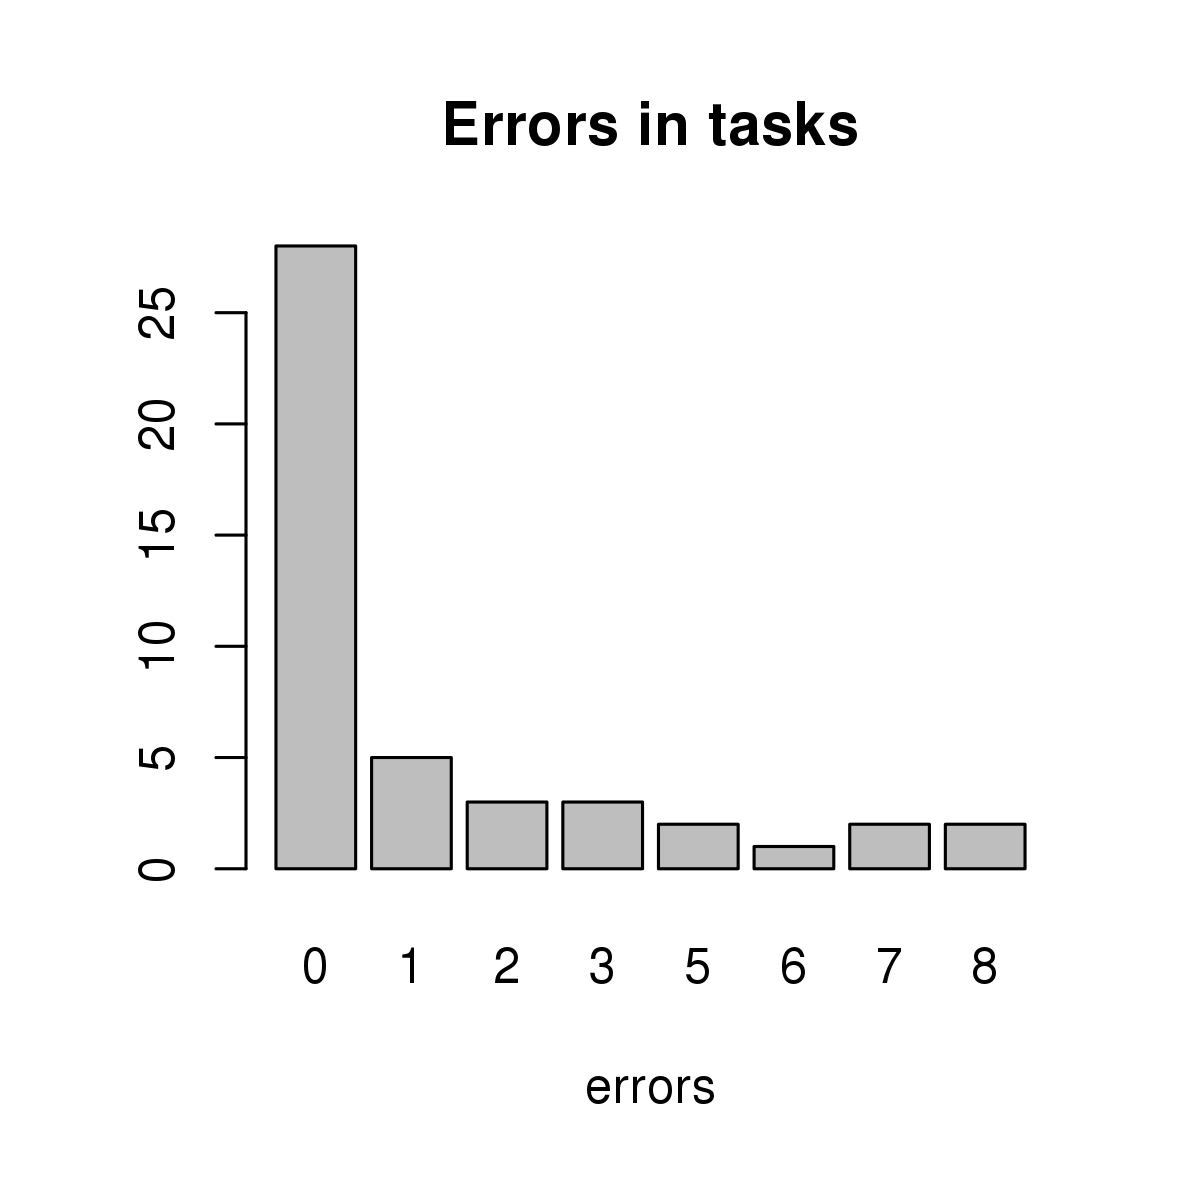
\includegraphics[width=0.99\textwidth]{pics/errors_in_tasks}
%\subcaption{xy}
%\end{subfigure}
%\begin{subfigure}[c]{0.5\textwidth}
%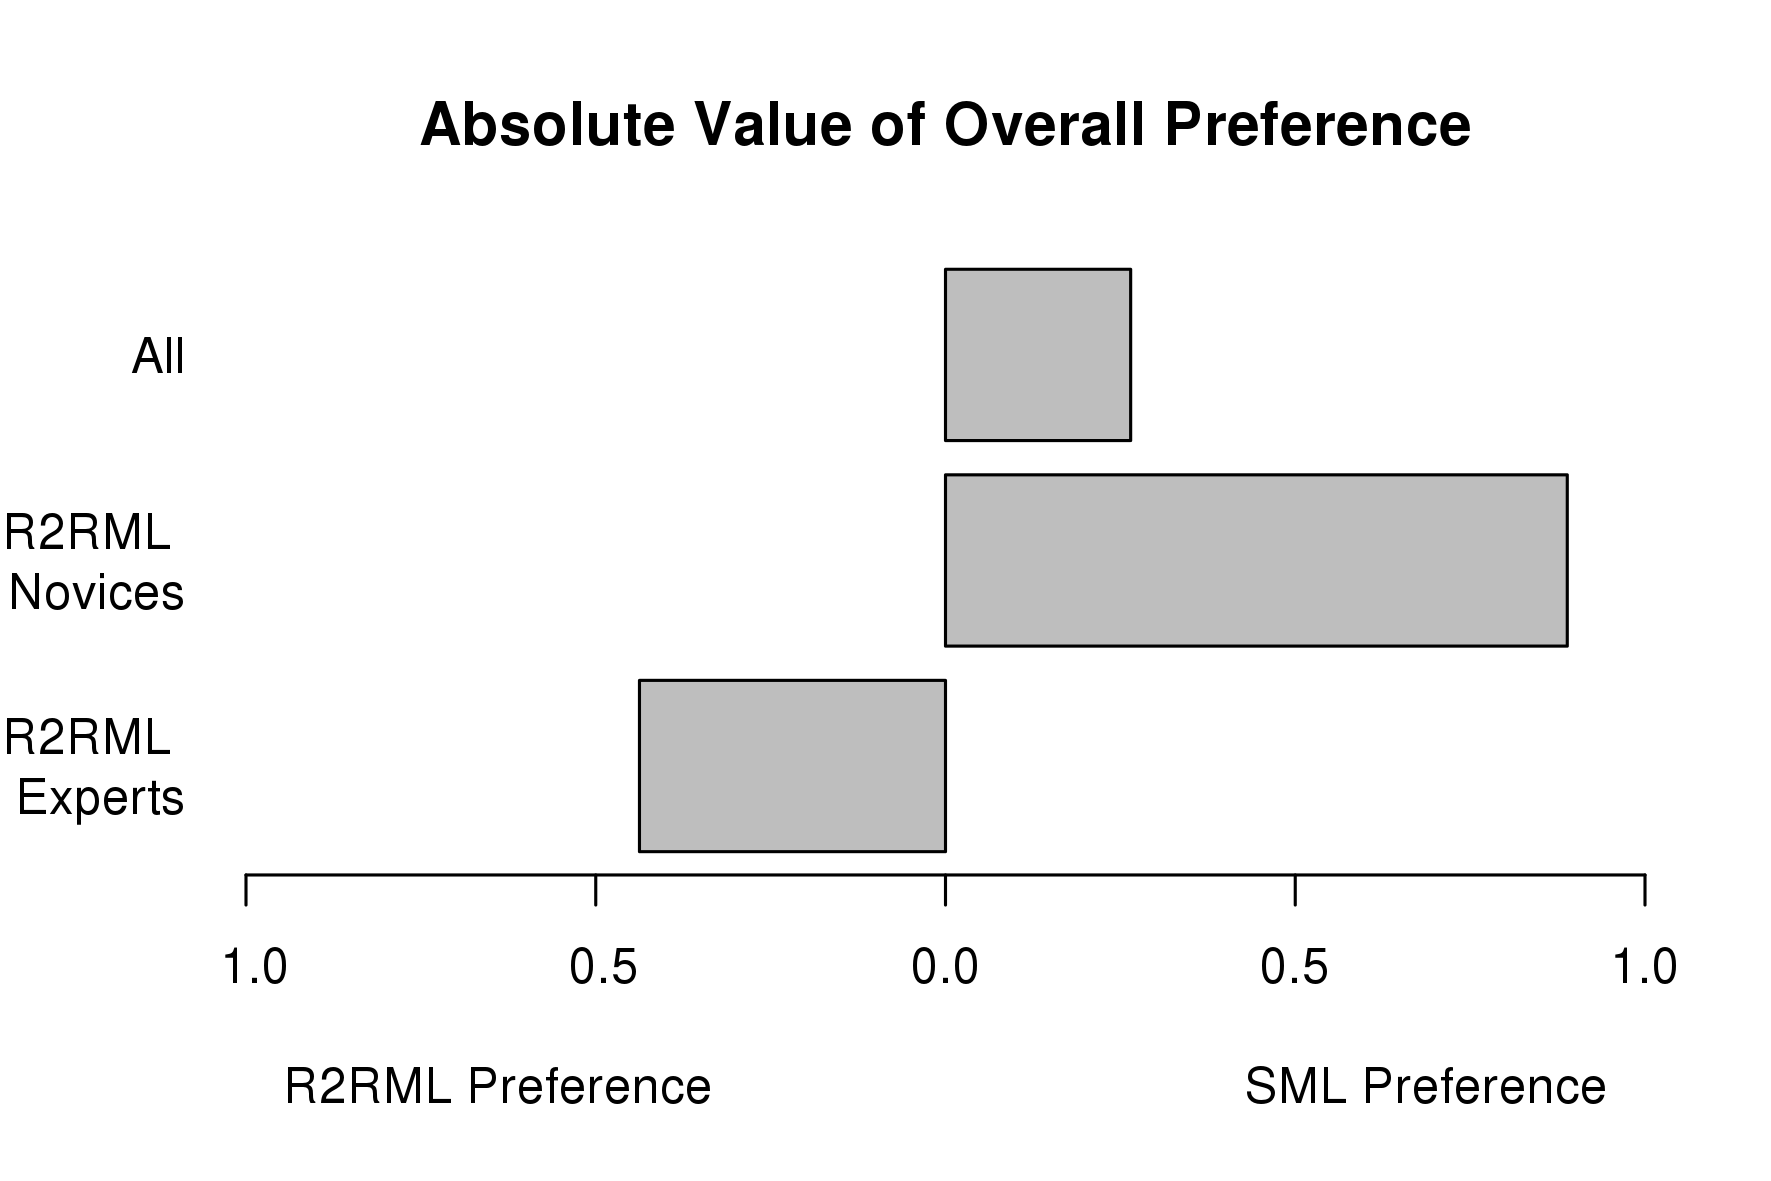
\includegraphics[width=0.99\textwidth]{pics/preference_exp_novice}
%\subcaption{xy}
%\end{subfigure}
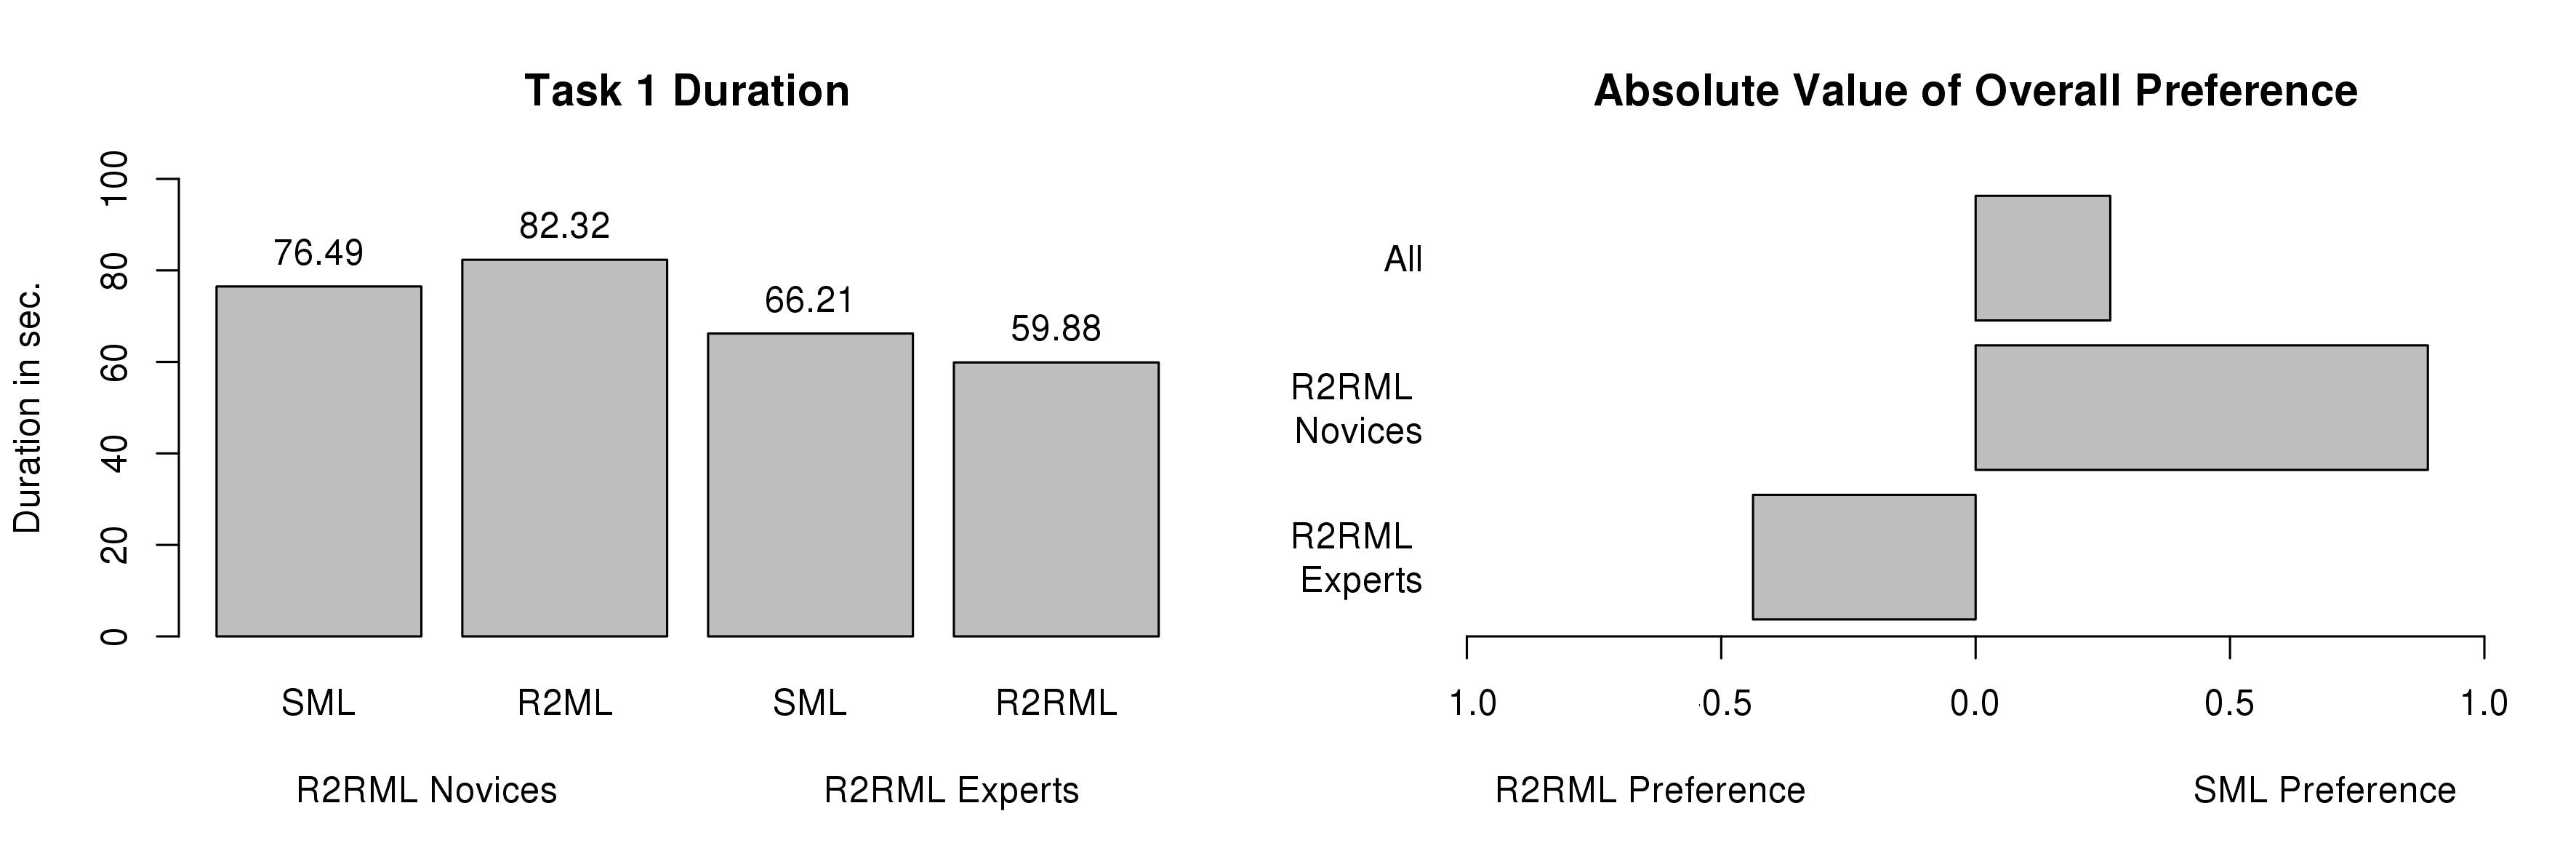
\includegraphics[width=\textwidth]{pics/time_n_pref}
%\vspace{-15pt}
\caption{The figure on the left assesses the time needed to solve an RDB2RDF mapping task. The figure on the right shows the preference for a mapping language. Overall, SML tasks required less time and the language was preferred, although this does not hold when considering only R2RML experts.}
\label{fig:time_n_pref}
\end{figure*}


We evaluated the SML mapping language to clarify the following questions:

\begin{compactenum}
 \item Is SML easier to read than R2RML and does SML have a lower entry barrier than R2RML?
 \item Can people understand SML mappings or R2RML mappings faster?
 \item If given the choice, would people prefer SML or R2RML?
\end{compactenum}

\subsection{Experimental Setup}

We set up a survey, which consists of three parts:

\begin{compactenum}
 \item Questions about prior expertise of the participant.
 \item Test questions for SML and R2RML.
 \item An assessment of the characteristics of SML and R2RML by the participants.
\end{compactenum}

We used a standard star rating for most questions ranging from 1 star (lowest value) to 5 starts (highest value).
The comparison with R2RML was performed as it is the current W3C standard for RDB2RDF mapping.

In the fist part, we asked participants to state their familiarity with the SML and R2RML languages as well as with related concepts such as the Turtle syntax and the SQL and SPARQL query languages.
In the second part, we had 5 different tasks for participants.
Each task was formulated for SML and R2RML with renamed classes and properties.
In the first 3 tasks, participants had to select the subset of 4 shown triples, which was actually generated from a given mapping.
The tasks were ordered by complexity of the mapping specification.
In the 4th and 5th task, the inverse needed to be performed:
Given a target RDF output, participants had to select those mappings from 4 presented mappings, which generates the target output.
Finally, in the third part of the survey, participants had to assess a) the difficulty of the presented tasks, b) whether they could make sense of the SML and R2RML mappings, c) whether they found SML and R2RML easy to read, d) whether they would consider using SML for RDB2RDF tasks and e) whether they have a preference between SML and R2RML.

The survey was distributed to the Semantic Web and Linked Data mailing lists and announced on Twitter.

\subsection{Results}
%\vspace{-5mm}




Overall, a total of 102 participants took part in the survey, of which 73 completed the survey.
We removed entries with an completion time below 500 seconds in order to remove bot entries and carefully assessed the removed entries.
46 participants remained out of which 28 answered all test questions correctly.
The 46 participants required an average time of 1243.1 seconds to complete the survey.
As a result, the overall time valid participants spent on the survey was 953 minutes.
All results of the survey can also be directly obtained and analysed at the SML project website.

The averaged results of the survey are shown in Table~\ref{tab:eval_overview}.
The self assessment scores in Table~\ref{tab:eval_overview} illustrate that the audience is interested in RDB2RDF conversions and that the participants are familiar with Turtle (TTL), SPARQL and SQL.
R2RML familiarity is considerably lower with an average of 3 and SML relatively unknown (1.74).

We discuss each of our evaluation questions in turn:

\emph{Readability and Entry barrier:} Figure~\ref{fig:fam_vs_read} shows that SML appears to have a lower entry barrier than R2RML.
Participants who were familiar with R2RML already judged both languages to have similar readability.
However, participants who were less familiar with R2RML judged SML to be much more readable than R2RML and gave high readability scores.

\emph{Time needed to solve tasks:}
For this task, we randomly started the survey either with either an SML or R2RML task to be able to assess this evaluation question.
The median time required for completing completing in R2RML was 67.08 seconds and for SML 69.23 seconds, giving R2RML a slight edge.
In a more thorough analysis, Figure~\ref{fig:time_n_pref} shows the time required to solve the first RDB2RDF mapping task in the survey, for R2RML experts (self assessment greater or equal 4) and R2RML novices (self assessment less 4).
R2RML experts require less time for solving the task in the R2RML, however R2RML novices appear are able to complete the task faster using SML.
It is further clear that R2RML experts require less time for solving the task regardless of the utilized language.
It should be noted that there is an unknown amount of time required to understand the task irrespective of the mapping language, i.e.~the difference between the mapping language is larger than depicted.


\emph{Overall preference:} Figure~\ref{fig:time_n_pref} shows that there is an overall preference for SML. This preference does not hold when considering only the group of R2RML experts, but is very significant when considering people not familiar with any of the two mapping languages.


\section{Conclusions and Future Work} %no future work so far (not strictly needed) %  and Future Work} \todo{[Claus,Jens]}
\label{sec:conclusion}
%\vspace{-5mm}
In this article, we presented work towards a unified model for RDB2RDF mappings and the
lightweight mapping language \emph{SML} that reuses familiar elements of SPARQL
and SQL in order to lower the learning curve and ease the manual writing and maintenance of view definitions.
An extensive public survey confirmed that this is the case.
%\todo{R3: would need to be supported with a usability study}
We provided an in-depth comparison of how SML relates to the R2RML standard, and
detailed how the former can be automatically converted to the latter.
%A comprehensive formalization of the RDB-RDF rewriting process based the
%definition of RDF views of a relational database and bindings, which bridge
%between the relational and SPARQL algebra.

SML has been successfully deployed in several scenarios:
We created SML mappings for the BSBM and SP2 benchmarks, two
popular SPARQL benchmarks that are often used for evaluating RDB2RDF
mappers.
Most prominently, we created SML mappings for transforming the
OpenStreetMap (OSM) database to RDF. These efforts are carried out
as part of the LinkedGeoData\footnote{\url{http://linkedgeodata.org/}} (LGD) project,
where we give access to more than 25 billion OSM RDF triples created through
SPARQL-to-SQL rewriting over about 3 billion relational rows via more than 40
SML view definitions.

%LGD also includes mappings for the GADM dataset
Furthermore, SML mappings have been created for two large scale
linguistic resources: One is the mapping of the Wortschatz
database\footnote{\url{http://www.wortschatz.uni-leipzig.de/}}, which contains
statistics, such as frequency and co-occurrences, about words in more
than 240 languages.
The other resource is PanLex\footnote{\url{http://ld.panlex.org}}, which is
a database holding translations of about 19 million expression extracted from
over 2.000 sources. Links to the corresponding SML mappings are published
together with our other SML related
resources\footnote{\url{http://sml.aksw.org}}.

In general, we believe that mapping relational structures to RDF will stay a highly important topic in research and practice to provide an unobtrusive transition towards the use of semantic technologies.
Providing engineers an intuitive yet powerful language is a crucial step to ease this transition.
Future work will continue on extending the formalizations as well as sorting out details based on community feedb,
such as whether an explicit \texttt{FROM QUERY} syntax for specifying SQL queries is preferred over
the current approach where this is implied by the use of triple quotes.

%\todo{R2: The weakness of SML also should be discussed}
%\url{http://sml.aksw.org}.
%Todo factor out the sml parser
%This work is the first step in a larger research agenda:
%In the future, we aim to remove even more barriers between the relational and
%RDF worlds.
%Currently, our mapping approach one-directional and read-only: queries are
% translated from SPARQL to SQL and query results from SQL to SPARQL.
%In the future, we plan to make the RDB-RDF mapping writable by enabling SPARQL
% updates, which are translated into updates of the underlying relational database.
%An interesting research direction, for which our formalization could be
% exploited, are bi-directional and hybrid mapping allowing an RDBMS to access RDF data and a possible incorporation of relational and RDF sources in a single mapping.
%A further research question is how inferencing and reasoning features can be
% integrated into the RDB-RDF mapping and rewriting.
%Another issue in this regard is how the SPARQL 1.1
% features\footnote{\url{http://w3.org/TR/sparql11-query/}}, such as property paths of arbitrary length, can be efficiently supported in the SPARQL-SQL rewriting.
%Furthermore, although we believe that SML is easier to use while offering similar functionality and expressiveness as R2RML
%the RDF based mapping language R2RML\footnote{\url{http://w3.org/TR/r2rml/}}, % no need for the full name and URI here after mentioning R2RML a hundred times ;)
%the latter has been standardized very recently and should therefore be supported by the Sparqlify system.
%Yet, we believe that Sparqlify-ML is in most cases easier to learn and use than R2RML, and therefore see future efforts on improving Sparqlify-ML as complementary.


% Jens: I removed the last part as it was just stating that Sparqlify should support R2RML, which is not the point of the article.

%\section*{Acknowledgment}
%\vspace{-5pt}
%This work was supported by grants from the EU's 7th Framework Programme provided for the projects LOD2 (GA no. 257943) and GeoKnow (GA no. 318159).

%\vfill
%\columnbreak

%\bibliographystyle{abbrv}
%\bibliography{../../bib/aksw,literature}






\section{Introduction}
RML (RDF Mapping Language) and SPARQL (SPARQL Protocol and RDF Query Language) are two important tools in the construction of knowledge graphs and the Semantic Web.
RML is an RDF-based language used for mapping data from different sources to RDF. It allows developers to transform and integrate data from various formats such as CSV, JSON, and XML into RDF triples.
SPARQL is an expressive query language used to retrieve data from RDF triple stores. Its federated query feature allows developers to write complex queries that can retrieve data from multiple sources.
%Together, RML and SPARQL play a crucial role in the construction of knowledge graphs, which are used to represent and interlink data from multiple sources, creating a more comprehensive view of a particular domain.
%As the amount of data on the web continues to grow, the use of RML and SPARQL is becoming increasingly important for
%enabling 
%the creation of large knowledge graphs.
%powerful applications.
So far, both approaches are treated as different: On the one hand there are tools specifically for
processing RML whereas on the other hand there are tools that extend SPARQL in order to incorporate additional data sources.
The motivation for this work is to devise a unified approach to the problem of large-scale knowledge graph construction.
%One of our visions is to enable research into the extent to which findings from SPARQL (query) execution optimizations can be leveraged for RML and vice versa.

The contributions of this work are: (1) We present an approach to translate RML to SPARQL with corresponding optimizations.
(2) We introduce the \emph{Not Only RDF SPARQL Extensions} (NORSE) for processing CSV, JSON and XML.
%JenaX features several extensions that can be plu into Apache Jena's ARQ query engine.
These extensions comprise additional functions and special SERVICE implementations with IRIs in the ``\texttt{norse:}'' namespace \texttt{https://w3id.org/aksw/norse\#}.
 The implementations are part of our JenaX resource\footnote{\url{https://github.com/Scaseco/jenax}} which is available on Maven Central. It features several unofficial extensions for the Apache Jena framework.
(3) We furthermore present an Apache Spark-based SPARQL engine that executes NORSE-enhanced SPARQL by leveraging its massive parallel processing model. We show that performance- and scalability-wise this approach surpasses the state of the art in several scenarios.
It is worth noting that achieving these results is not the sole merit of Apache Spark, but also that of the optimizations we used.

The remainder of this paper is structured as follows:
We present related work
%about mapping languages and tools in the knowledge graph domain
in~\Cref{sec:related-work}.
The translation of RML models to extended SPARQL CONSTRUCT queries is described in~\Cref{sec:rml-to-sparql}.
Optimizations of query workloads with respect to the uniqueness and ordering of the produced RDF triples and/or quads are shown in~\Cref{sec:optimize}.
In \Cref{sec:implementation} we present our implementations for (1) converting RML to SPARQL (2) the NORSE SPARQL extensions
% for Apache Jena's ARQ query engine
and (3) the implementation of a SPARQL engine on Apache Spark using the SANSA Big Data RDF framework.
Subsequently, in~\Cref{sec:eval} we present an evaluation of our approach based on the GTFS Madrid Bench and one dataset of the SDM Genomic Datasets.
%We also discuss which parts of our approach have not yet worked ideally.
We conclude our paper in~\Cref{sec:conclusions}.

The implementation of our approach is part of our RDF Processing Toolkit (RPT)\footnote{\url{https://github.com/SmartDataAnalytics/RdfProcessingToolkit}} which is based on JenaX.

%and point out future work.
%\todo{Provide a link to the tool here}

\section{Related Work}
\label{sec:related-work}
In this section we provide an overview of contemporary SPARQL and RML based knowledge graph construction approaches 
%mapping languages, RML processors, %benchmarks 
as well as a brief summary of Apache Spark.
As there exist many mapping languages\cite{Meester2019, ChavesFraga2021, IglesiasMolina2022a, Assche2023}, a discussion of general concepts and translations between them can be found in \cite{Corcho2020, IglesiasMolina2022}.

%\citet{Corcho2020} and \citet{IglesiasMolina2022}.
%Mapping of data to RDF graphs is usually either done with custom implementations, direct mappings, or using dedicated mapping languages\citep{Dimou2020}. 

%and the parallelization framework Apache Spark.

%\subsection{Mapping Languages}
\subsection{SPARQL-based Mapping Approaches}
%In this article we are focusing on later and especially R2RML\footnote{\url{https://www.w3.org/TR/r2rml/}}, RML\cite{Dimou2014} and SPARQL.
%\todo{I hope I replaced sparql integrate with NORSE correct. Lars-Peter}.
%There are several articles \citep{Meester2019, ChavesFraga2021, IglesiasMolina2022a, Assche2023} on the different mapping languages.
% The most relevant seem to be R2RML\citep{Das2012}, RML\citep{Dimou2014}, SPARQL Generate\citep{lefranccois2017sparqlgenerate}, YARRRML\citep{heyvaert2018declarativeyarrrml} and ShExML\citep{GarciaGonzalez2021}.
%\subsection{R2RML and RML}
%\todo{cite our ldow 2015 paper}.
%R2RML and RML are categorized by  \citet{IglesiasMolina2022a} as "RDF-based".
%Beside the "RDF-based"\cite{IglesiasMolina2022a} R2RML and RML we want to outline SPARQL. 
%\subsection{SPARQL}
%is a recursive acronym for \emph{SPARQL Protocol and RDF Query Language} and
\emph{SPARQL} is a W3C standard for processing (loading, retrieving, transforming and updating) RDF data\footnote{\url{https://www.w3.org/TR/sparql11-query/}}.
%Consequently, \emph{SPARQL engines} are systems that can evaluate \emph{SPARQL statements}.
SPARQL engines can be leveraged to build advanced features on top.
%feature extension points.
Two prominent representatives of the category of SPARQL-based mapping approaches are SPARQL-Generate\cite{lefranccois2017sparqlgenerate} and SPARQL Anything\cite{10.1145/3555312sparqlanything}.
SPARQL Anything extends SERVICE evaluation such that references to remote non-RDF data can be made. The data is converted to an opinionated RDF graph (as per documentation) which then serves as the base for evaluating the remainder of the SERVICE clause.
%It is noteworthy that as an effort to
SPARQL-Generate features a SPARQL-based template language which can produce output beyond what is possible with conventional SPARQL.

Our JenaX project compares to these approaches as follows: JenaX provides (among other things) SPARQL plugins for the Apache Jena ecosystem that allow for processing heterogeneous data within the SPARQL syntax already supported by the framework.
As part of this effort we contributed a plugin system to facilitate interoperability of custom SERVICE execution implementations\footnote{\url{https://github.com/apache/jena/pull/1388}}. 
The SPARQL extensions for processing RML sources, as described in this paper, are built on this system.
While some of JenaX's SPARQL extension functions for XML, JSON and CSV processing conceptually overlap with those provided by SPARQL-Generate, there are yet differences in the implementations. For example, JenaX provides dedicated RDF datatype implementations that internally retain JSON and XML data in an object model, whereas SPARQL-Generate (as of version 2.0.12) falls back to string representations.
In order to avoid clashes we use IRIs in the \emph{norse} namespace for our implementations.

%functions in SPARQL-Generate (2.0.12) always (re-)parse XML and JSON data from string whereas
%SPARQL-Generate (2.0.12) functions
%For example, JenaX supports dedicated RDF datatype implementations that internally retain JSON and XML data in an object model.  SPARQL-Generate (2.0.12) functions
%For example, JenaX supports dedicated RDF datatype implementations for JSON and XML that internally store the data in an object model which can be leveraged and the performance characteristics.
%For example, JenaX provides RDF datatype implementations that internally store JSON and XML in an object model in order to allow for fast operations whereas SPARQL-generate functions so far currently parse and produce strings.
%For example, JenaX features specialized RDF datatype implementations that internally represent JSON and XML in an object model rather than strings. 

%\todo{finish}
%The \emph{Not Only RDF SPARQL Extensions} (NORSE) SPARQL extensions introduced in \Cref{sec:NORSE} add support for CSV and JSON input.
%There are several ways to express extensions:\addtocounter{footnote}{-3} %3=n
%\stepcounter{footnote}
%Magic triples, Comments (\#pragma) RDF Reasoning in stardog.

\subsection{RML Processors and Benchmarks}
\emph{R2RML} is a W3C standard and vocabulary for mapping relational data to RDF\footnote{\url{https://www.w3.org/TR/r2rml/}}.
On the one hand these mappings can be used in ETL processes to dump databases as RDF. On the other hand, the same mappings can be used in SPARQL-to-SQL rewriting, a.k.a. OBDA (ontology-based data access). While R2RML is considered quite verbose, several alternatives have been developed, such as the Stardog Mapping Syntax (SMS, currently in version 2), the Ontop Mapping Language\cite{calvanese2017ontop}, and the Sparqlification Mapping Language\cite{stadler2015simplified}.

\emph{RML}\footnote{\url{https://rml.io/specs/rml/}} is an extension of R2RML which adds additional vocabulary for mapping non-relational data\citep{Dimou2014, Dimou2020}. In essence these additional declarations allow for expressing a mapping of non-relational data (such as XML and JSON) into a relational model where from each row RDF tuples are generated. Like R2RML it suffers from verbosity, for which reason simplified models were derived such as YARRRML\cite{heyvaert2018declarativeyarrrml}.
A mapping translation between ShExML\cite{GarciaGonzalez2021} and RML is presented by \cite{GarciaGonzalez2022}.

There exist several RML processors \cite{ArenasGuerrero2021, Iglesias2023}\footnote{\url{https://github.com/kg-construct/awesome-kgc-tools}} for the well known extension RML of the W3C standard R2RML. 
%\citet{ArenasGuerrero2021} gives an overview on the state of the art and compares them using the Madrid GTFS benchmark.
%\citet{Iglesias2023} introduces some optimization and compares the RML processors RMLMapper, RocketRML, Morph-KGC and SDM-RDFizer using the Madrid GTFS benchmark and the SDM-Genomic-Datasets.
In this paper we are comparing benchmarks with the following: %Morph-KGC and SDM-RDFizer.
\emph{SDM-RDFizer}\footnote{\url{https://github.com/SDM-TIB/SDM-RDFizer}} is an RML processor implemented in python with optimized data structures and operators. It is developed with scalability and complex data in mind\cite{Iglesias2020}.
\emph{CARML}\footnote{\url{https://github.com/carml/carml}} and RMLMapper\footnote{\url{https://github.com/RMLio/rmlmapper-java}} are Java implementations which operate single threaded at the time of writing.
% TODO \emph{RMLStreamer} is a Flink-based implementation however upon writing the standalone container would not work so we deployed it on a cluster but on GTFSbench it would suffer from the missing self-join elimination. We decided to only benchmark the tools that could be used standalone.
\emph{Morph-KGC}\footnote{\url{https://github.com/morph-kgc/morph-kgc}} is an RML processor implemented in python and supports partitioning RML assertions\cite{arenas2022morphkgc} for parallel execution.

%and \emph{RMLStreamer}\cite{Haesendonck2019} are Java-based RML mappers.
%making use of input streaming.

%RML-conformance-test
%RML extension for excel
%RMLMapper / RMLStreamer: Similar tools, essentially the latter adds support for streaming input sources.
%Ontop\citep{calvanese2017ontop}


%\subsection{RML processor benchmarks}
For measuring the performance of the RML processors we use the following benchmarks:
The \emph{Madrid GTFS benchmark}\footnote{\url{https://github.com/oeg-upm/gtfs-bench}} was introduced by \cite{chaves2020gtfs}.
It is based on data from subway network of Madrid and the benchmark data can be scaled up.
A survey on RML tools\cite{ArenasGuerrero2021} conducted in 2021 evaluated 3 virtualizers and 6 materializers on the GTFS Madrid Benchmark.
% Madrid GTFS benchmark\footnote{\url{https://github.com/oeg-upm/gtfs-bench}}\cite{chaves2020gtfs} and the SDM-Genomic-Datasets benchmark\footnote{\url{https://figshare.com/articles/dataset/SDM-Genomic-Datasets/14838342/1}}.
The \emph{SDM-Genomic-Datasets benchmark}\footnote{\url{https://figshare.com/articles/dataset/SDM-Genomic-Datasets/14838342/1}} was introduced by \cite{Iglesias2020}.
This benchmark is motivated from the biomedical domain and based on the Catalogue Of Somatic Mutations In Cancer\footnote{\url{https://cancer.sanger.ac.uk/cosmic}}.
    
%\begin{itemize} \label{sec:benchmarks}
    %\label{sec:bench-madrid}

    % The evaluation suggests that at this time no system was capable of running the GTFS1000 benchmark within a 24 hours time limit.
    % This is no longer the case in 2022 work!

%    \label{sec:bench-sdm}

%\end{itemize}

%There are individual evaluations used as well, like the RMLStreamer benchmark suite \footnote{\url{https://github.com/s-minoo/rmlstreamer-benchmark-rust}} used with RMLStreamer\citep{Oo2022RMLStreamerSISO}.

%Berlin Sparql Benchmark: probably not relevant here

\subsection{Apache Spark And SANSA}
Apache Spark\footnote{\url{https://spark.apache.org/}} is a framework for high parallelisation. It can scale workload execution from a single node to big clusters. Apache Spark advanced Hadoop's Map-Reduce paradigm with an abstraction called "resilient distributed datasets" (RDDs).
%\cite{Zaharia2010SparkCC}.
The SANSA framework\cite{lehmann2017distributed} is an effort to enable various forms of RDF processing on Apache Spark.
%\todo{cite lehmann2017distributed as it is referenced nowhere else}

\section{Translating RML to SPARQL}
\label{sec:rml-to-sparql}
In this section we describe our approach to translate RML to SPARQL.
For this purpose we first briefly summarize the notion of a SPARQL CONSTRUCT query.
%In the course of this section we also introduce SPARQL extensions for operating on heterogeneous data which we refer to as \emph{Not Only RDF Sparql Extensions} (NORSE).

\subsection{CONSTRUCT Queries}
A CONSTRUCT query has the form \lstinline|CONSTRUCT { template } WHERE { pattern }|.
Without loss of generality, for this work we assume generalized RDF\footnote{\url{https://www.w3.org/TR/rdf11-concepts/\#section-generalized-rdf}}.
Let there be the pairwise disjoint sets of IRIs $I$, blank nodes $B$ and literals $L$.
The set of \emph{RDF terms} is defined as $T := I \cup B \cup L$. Furthermore, let there be another set of SPARQL variables $V$. We define the set of \emph{SPARQL terms} $S := T \cup V$.
A {concrete} triple is an element of $T \times T \times T$ whereas a triple pattern is an element of $S \times S \times S$.
Likewise, a {concrete} quad is an element of $T \times T \times T \times T$ whereas a quad pattern is an element of $S \times S \times S \times S$.
The current SPARQL standard only allows for a CONSTRUCT template to specify the creation of triples using triple patterns.
However the importance of this issue has been noted\footnote{\url{https://github.com/w3c/sparql-12/issues/31}}
and several engines already support the production of quads as well.
The approach presented in the following can be used in either setting, so instead of talking about a triple and quad (pattern) we generally speak of a \emph{tuple} (pattern).
A construct query's template is thus made up of a set of tuple patterns. Substituting all variables of these tuple patterns with RDF terms thus produces a set of \emph{concrete} tuples.

%\todo{clean up}
%Other mappings available as well:
%general article: \citep{IglesiasMolina2022}
%ShExML to RML: \citep{GarciaGonzalez2022}
%Grafikeidee: yarrrml -> RML, shexml -> RML -> sparql

\subsection{Translating RML Logical Sources}\label{sec:NORSE}
The two main issues that need to be solved are how to translate (1) RML sources and (2) RML references to SPARQL elements.
RML sources conceptually emit a set of records whose attribute access is specified via \texttt{rml:reference}s.
On the SPARQL side, the \texttt{SERVICE} clause can be used to generate a set of bindings based on its contained pattern.
We can thus introduce a special SERVICE IRI \texttt{norse:rml.source} which contains a graph pattern that represents an RML source.
In addition, we add an additional triple pattern with the special predicate \texttt{norse:output} in order to bind the source records as RDF terms to a SPARQL variable.
%\todo{Move, rephrase or remove Paragraph below}
%Unfortunately, at present SPARQL lacks standardization for non-RDF datatypes and functions. Although RDF defines the datatype \texttt{rdf:XMLLiteral}, RDF frameworks
%do not necessarily implement it in a way that allows for e.g. efficient evaluation of XPath expressions\footnote{For example, Apace Jena stores XML literal internally as strings}.
Therefore, we introduce custom XML\footnote{Jena's implementation of the \texttt{rdf:xmlLiteral} datatype only stores XML as a string which is not suited for efficient XPath evaluation.} and JSON datatypes as well as corresponding functions, namely \texttt{norse:json} and \texttt{norse:xml} to capture XML and JSON data efficiently, respectively.


\begin{figure*}[htb]
\centering
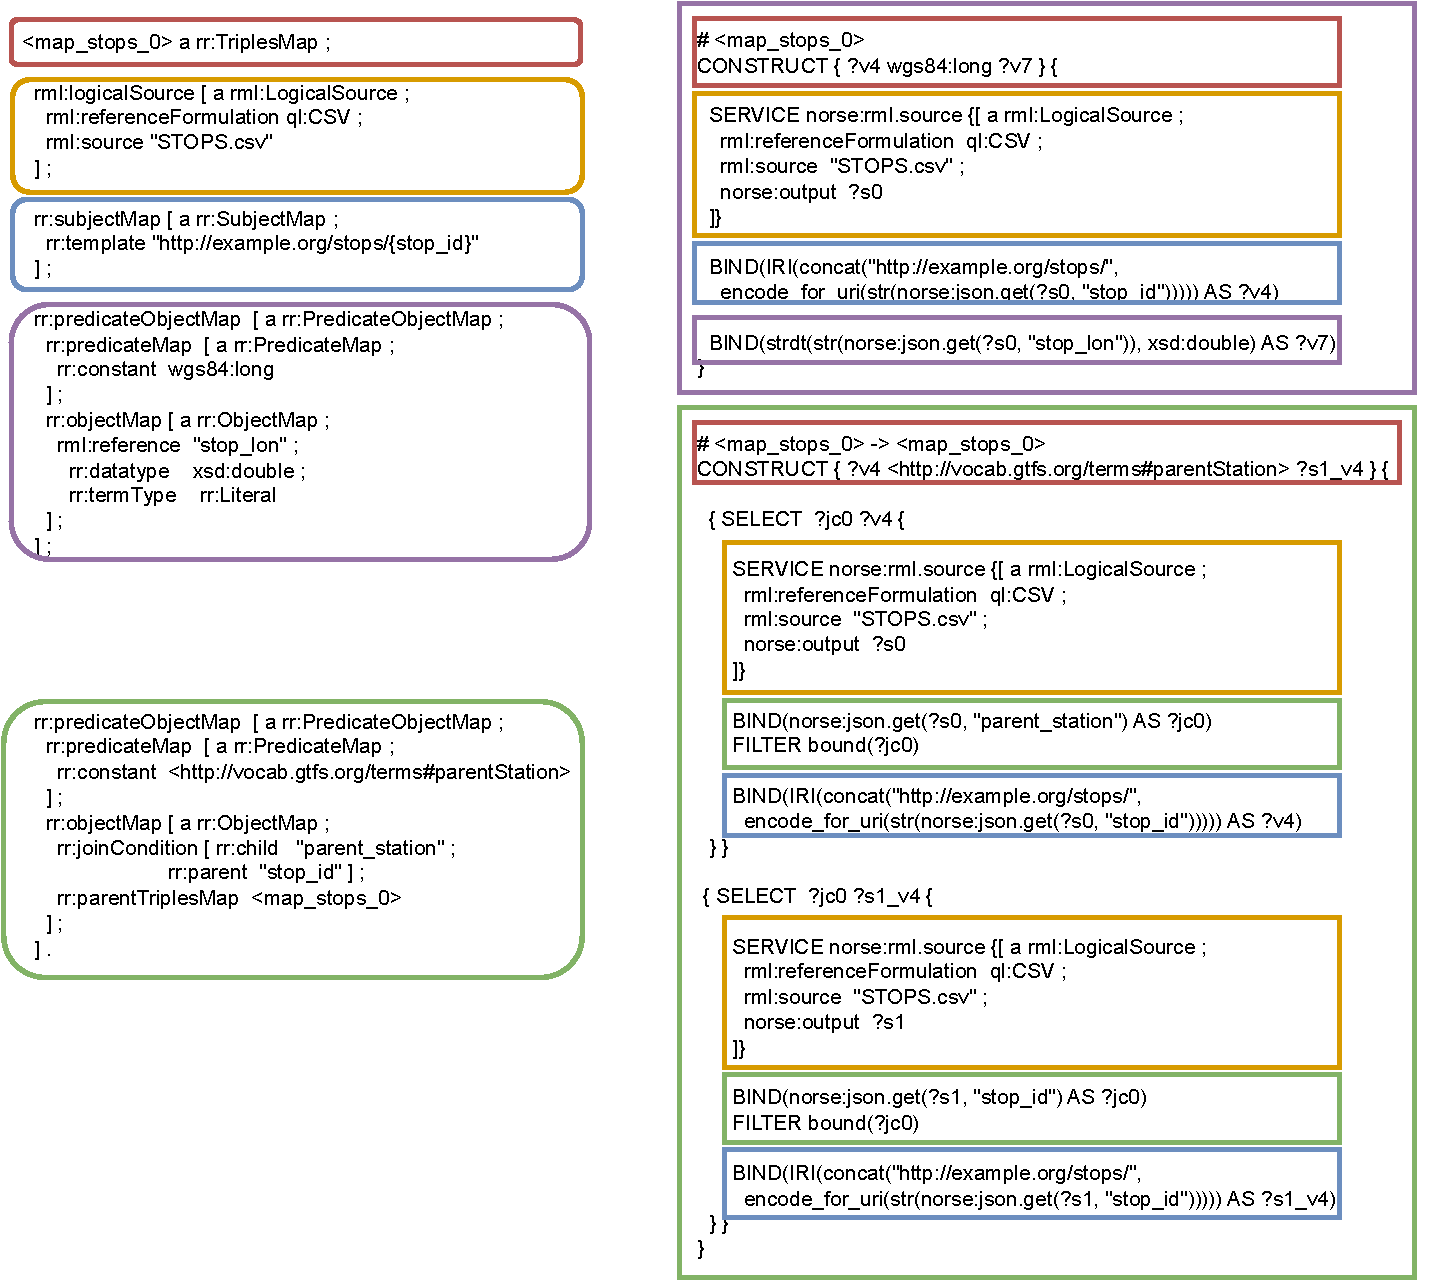
\includegraphics[width=0.9\textwidth]{images/rml-to-sparql.pdf}
%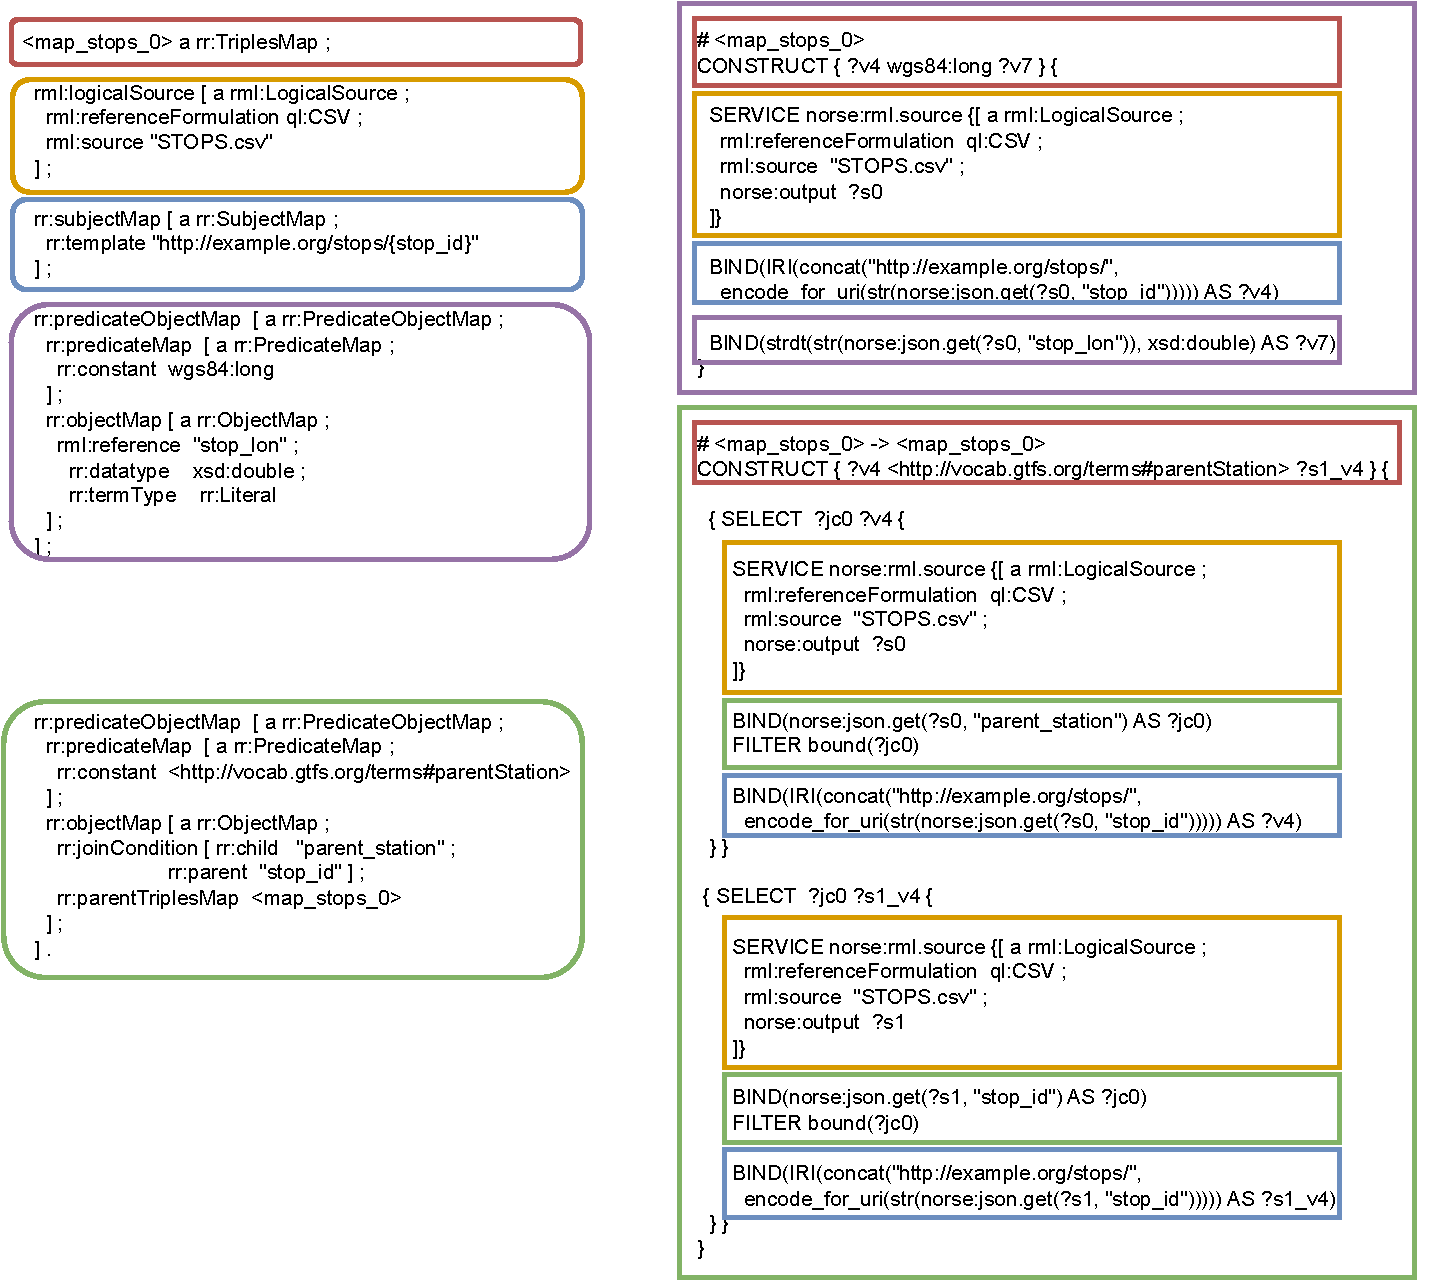
\includepdf[pages=-]{images/rml-to-sparql.pdf}
\label{fig:rml-to-sparql}
\caption{Juxtaposition of an RML document and its representation as SPARQL queries. The RML join condition is transformed into a natural join of SPARQL graph patterns where the same variable (\texttt{?jc0}) is bound on both sides.}
\end{figure*}

\subsection{Translating RML TermMaps}
RML TermMaps specify how to map the referenced data to RDF terms.
SPARQL operates at the level of bindings where variables are bound to RDF terms.
Hence, we can represent RML TermMaps in SPARQL by using \texttt{BIND} to define variables as expressions over a source's data.
SPARQL provides the functions \texttt{IRI}, \texttt{STRDT}, \texttt{STRLANG} and \texttt{BNODE}\footnote{Unfortunately the standard \texttt{BNODE} function is not deterministic so SPARQL-based knowledge graph construction tools typically either alter the semantics or provide an alternative function.} for the construction of RDF terms.
Consequently, every TriplesMap's term map can be represented using a freshly allocated variable that is bound to a corresponding definition using a SPARQL \texttt{BIND} statement. A summary for mapping RML term maps to SPARQL is shown in~\Cref{fig:tm-to-sparql}. The function \texttt{access} is thereby a placeholder that needs to be replaced with a concrete variant based on the type of the logical source (e.g. XML, JSON, CSV) as explained in~\Cref{sec:rml-ref-to-sparql}.

\begin{figure*}
\begin{footnotesize}
\begin{itemize}
%    \setlength\itemsep{-0.5em}
  %\setlength{\itemindent}{.5in}
  \item \lstinline{[ rr:reference "ref" ]} $\rightarrow$ \lstinline{BIND(access(?source, "ref") AS ?v0)}
  \item \lstinline{[ rr:reference "ref" ; rr:termType rr:IRI ]} $\rightarrow$ \lstinline{BIND(IRI(access(?source, "ref")) AS ?v0)}
  %\hspace{1cm}
  \item \lstinline{[ rr:reference "ref" ; rr:termType rr:BlankNode ]} $\rightarrow$
  
  \hspace{1cm}\lstinline{BIND(BNODE(access(?source, "ref")) AS ?v0)}
  \item \lstinline{[ rr:reference "ref" ; rr:datatype xsd:float ]} $\rightarrow$
  
  \hspace{1cm}\lstinline{BIND(STRDT(access(?source, "ref"), xsd:float) AS ?v0)}
  \item \lstinline{[ rr:reference "ref" ; rr:language "en" ]} $\rightarrow$
    
  \hspace{1cm}\lstinline{BIND(STRLANG(access(?source, "ref"), "en") AS ?v0)}
\end{itemize}
\end{footnotesize}
 \vspace*{-5mm}
\caption{Translating RML term maps to SPARQL BIND expressions.}
\label{fig:tm-to-sparql}
\end{figure*}

%  \hspace{1cm}\lstinline{BIND(STRLANG(access(?source, "ref"), "en") AS ?v0)}
%  \item \lstinline{[ rr:reference "ref" ; rml:languageMap [ rml:reference "lang" ] ]} $\rightarrow$ 


\subsection{Translating RML References}
\label{sec:rml-ref-to-sparql}
The concrete expression of the \texttt{access} function depends on the logical sources' format. Because the format is specified, we can rewrite \texttt{access} with the following concrete functions, where \texttt{REF} is substituted with reference expression string.%the argument to \texttt{access}: 
%RML references are translated to the following SPARQL functions:
\begin{itemize}
% NOTE!!! Overleaf incorrectly marks an error here, please do not correct!!!
    \item JSON: \lstinline{norse:json.path(?x, "$['REF']")} If the result of the JSON path evaluation is a primitive JSON object then it is converted to an RDF term. JSON null is treated as ``unbound''. For JSON arrays and objects an RDF term of type \lstinline{norse:json} is returned.
    \item CSV: In our approach we represent CSV rows as JSON documents and thus access could be performed using the aforementioned \texttt{norse:json.path} function.
    If headers are absent then every row is represented as a JSON array, otherwise every row is turned into a JSON object whose keys are the CSV headers.
    %TODO State that more configuration can be done with the CSVW model
    However, in order to avoid the overhead of JSON path evaluation we also introduce the function \lstinline{norse:json.get(?obj, "REF")} for accessing a JSON object's immediate keys directly.
    \item XML: \lstinline{norse:xml.text(norse:xml.path(?xmlNode, "//:REF"))} The result of an XPath evaluation is generally another XML node, such as \lstinline{<lon>42.5</lon>}. The function \lstinline{norse:xml.text} extracts an XML element's content as text, in this example \lstinline{42.5}.
\end{itemize}

%The datatype rule depends on the assumption that the IRI of the datatype can itself can act as a function call (which is the case for all standard SPARQL datatypes).

\subsection{Translating RefObjectMaps (Joins)}
Joins in RML are declared using \texttt{rr:RefObjectMap}. The outcome of the translation of an RML join is a CONSTRUCT query which involves a natural join based on the references to the sources that act as child and parent as shown in~\Cref{fig:rml-to-sparql}.
Every \texttt{rr:RefObjectMap} results in an independent CONSTRUCT query with only one tuple pattern in its template.

\subsubsection{Duplicate-Reducing Self Join Elimination}
%\todo{Can we describe it better here?}
%Without loss of generality, a TriplesMap 
%RefObjectMap represents a JOIN of two relations which are specified by the child and parent TriplesMaps.
% If either side's projected columns are a subset of the join key then we can remove the join.
%\[
%R \times S
%\]
For time-efficient execution of RML mappings, such as the ones used in the GTFS-Madrid-Benchmark, it is known that a form of self-join elimination must be performed\cite{Iglesias2020, arenas2022morphkgc}.
%Given an arbitrary relation, such as a CSV file, it is not generally possible to assert the uniqueness of columns because of the lack of metadata.
%(either from an external source or obtained using pre-processing), 
%is not directly possible to determine whether columns have unique values.
%As a consequence, schematic self-join elimination based on uniqueness constraints is typically not possible without prior computation of metadata.
%However,
An RML join condition can be generally omitted if the following conditions are met:
\begin{itemize}
    \setlength\itemsep{-0.5em}
%    \item The parent TriplesMap's logical source is the same as that of the child TriplesMap.
    \item The same logical source is used for the child and the parent TriplesMap.
    \item All involved join conditions use the same reference expression for both parent and child, such as \lstinline{rr:parent = "ref" ; rr:child "ref"}.
    \item Either of the subject maps only mentions a subset of the references used in the join.
\end{itemize}
In such a case a referencing object map can be replaced with a simple object map based on the referenced TriplesMap's subject map. The underlying principle is sketched as follows. Let $R$ be the TriplesMap's logical relation. Let $C$ and $P$ be the set of attributes referenced by the child and parent subject maps, respectively. Let $J$ be the set of joining attributes. Then the following transformation can be applied if the condition $P \subseteq J$ or $C \subseteq J$ is met (\texttt{c} and \texttt{p} are SQL aliases):

\lstinline[language=SQL,basicstyle=\footnotesize,mathescape=true]!SELECT DISTINCT $C \cup P$ FROM $R$ c JOIN $R$ p USING ($J$) $\rightarrow$ SELECT DISTINCT $C \cup P$ FROM $R$!

\noindent If the condition is met but DISTINCT is omitted then the JOIN can only introduce additional duplicates. Applying the transformation then reduces the duplicates to only those present in $R$.

%the result sets of either side will evaluate to the same set of tuples, however the right hand side may assign them lower cardinalities thus reducing duplicates.
%$\xrightarrow{P \subseteq J \vee C \subseteq J}$
%\end{lstlisting}
%\todo{Add example - maybe juxtpose with one where this does not work}
%Note, that this is not an equivalence transformation as it may reduce the cardinalities of bindings in the result set.
%Note, that without \texttt{DISTINCT} is holds that the evaluation of the right hand side (with the eliminated join) yields a sub set of that of the left hand one.
%in the worst case the cardinalities remain the same.

\section{Optimizing SPARQL CONSTRUCT Query Workloads}
\label{sec:optimize}
By transforming RML mappings into a set of SPARQL queries, the problem of efficient RML mapping execution becomes one
of workload optimization of a set of SPARQL CONSTRUCT queries.
The essential optimization goals are to efficiently produce tuples that are
unique and/or ordered: For RDF data it is desirable to avoid duplicates as they needlessly increase size and processing time.
Sorted RDF data eases inspection of the available information and assessment of fitness for use. It also enables efficient lookups using e.g. binary search. In the remainder of this section we detail our employed optimization procedure.

%produce a uniqueness and ordering of the produced tuples.
%A problem with SPARQL 1.1 is that it does not directly provide DISTINCT and ORDER BY operators for CONSTRUCT queries. Fortunately, a recent advancement towards the next version of SPARQL is the introduction of \texttt{LATERAL}. This feature makes it possible to convert CONSTRUCT queries into equivalent SELECT ones that project three or four variables (for triples or quads, respectively) as shown in the remainder.
% as well as leveraging early adopting implementations 

\subsection{Merging CONSTRUCT Queries using LATERAL}
There are two main issues with SPARQL 1.1 CONSTRUCT queries for the purpose of producing sorted and unique knowledge graph output:
\begin{itemize}
%    \setlength\itemsep{-0.5em}
    \item Although ORDER BY and/or DISTINCT can be used with CONSTRUCT queries, these solution modifiers only affect the underlying bindings and not the produced tuples. This is especially an issue when a CONSTRUCT query's template mentions multiple RDF tuple patterns.
    With SPARQL 1.1 there is no generic procedure to compute unique tuples in an efficient way that only has to evaluate the query pattern once.
    \item While multiple SELECT queries can be combined with UNION, no such operator exists for CONSTRUCT queries.
\end{itemize}

These two issues make it difficult to devise a general procedure to efficiently combine tuples generated by a set of CONSTRUCT queries.
A recent effort towards the next version of the SPARQL specification is the introduction of the \texttt{LATERAL} keyword which is already supported by a few SPARQL engines\footnote{\url{https://github.com/w3c/sparql-12/issues/100}}.
%A recent (non-standard) addition to some SPARQL engines led to the introduction of the \emph{LATERAL} keyword and the corresponding binary algebraic operator.
The keyword's corresponding operation first evaluates the left-hand-side. Each obtained binding is then used to substitute all (in-scope) variables on the right-hand-side before the substituted right-hand-side is evaluated:
\[
[[\mathtt{Lateral}(\mathtt{left}, \mathtt{right})]] := \left\{\mu_l \cup \mu_2 | \mu_1 \in [[\mathtt{left}]] \mathtt{\:and\:} \mu_2 \in [[\mathtt{subst}(\mathtt{right}, \mu_1)]]\right\}
\]
With this keyword it is now possible to ``normalize`` \emph{any} CONSTRUCT query into an equivalent one with a canonical template of the form
\lstinline|GRAPH ?g { ?s ?p ?o }|
for quad-based approaches or \lstinline{?s ?p ?o} for triple-based ones. Without loss of generality, any clashes in variable naming can be resolved with appropriate renaming.
This way, a set of normalized CONSTRUCT queries can be UNION'd simply by creating a UNION of their graph patterns and adding the uniform template.
The operations ORDER BY and DISTINCT can be applied likewise.
%it is finally possible to express uniqueness on construct queries as show in\Cref{fig:construct-to-lateral}.
The general CONSTRUCT-to-LATERAL rewrite is described in~\Cref{fig:construct-to-lateral}.
Note, that \texttt{DEFAULT} is thereby an implementation dependent constant for the default graph\footnote{See discussion \url{https://github.com/w3c/sparql-12/issues/43}}.
Given a set of CONSTRUCT queries, a generic \emph{merge} can be accomplished based on their lateral form as shown in~\Cref{fig:combine-lateral}.

%, and \texttt{CONSTRUCT} with graph patterns .

%Evaluation of a CONSTRUCT query evaluates its involved graph pattern as a SELECT query and using each obtained binding to instantiate the tuple patterns of the template. 
%However, with SPARQL 1.1 it is not easily and/or efficiently possible to generally express uniqueness of the produced tuples.
% However, some engines already support features that will likely make it into the SPARQL 1.2 specification
%Even though SPARQL 1.2 is


\begin{figure*}[!h]
 \begin{minipage}[t]{0.29\textwidth}
  \centering
  \begin{lstlisting}[language=SPARQL]      
CONSTRUCT {
  s1 p1 o1
  ...
  GRAPH gn { sn pn on }
} WHERE
  PATTERN
}
  \end{lstlisting}
%  \caption{listing}{Sub caption}
 \end{minipage}
 \begin{minipage}[t]{0.69\textwidth}
  \centering
  \begin{lstlisting}[language=SPARQL]
CONSTRUCT { GRAPH ?g { ?s ?p ?o } }
WHERE {
  SELECT DISTINCT ?g ?s ?p ?o {
    PATTERN
    LATERAL {
        { BIND(DEFAULT AS ?g)
          BIND(s1 AS ?s) BIND(p1 AS ?p) BIND(o1 AS ?o) }
      UNION
        ...
      UNION
        { BIND(gn AS ?g)
          BIND(sn AS ?s) BIND(pn AS ?p) BIND(on AS ?o) }      
    }
  } ORDER BY ?s ?p ?o ?g
}
  \end{lstlisting}
%  \caption{listing}{Another sub caption}
 \end{minipage}
 \vspace*{-5mm}
 \caption{Rewrite of a CONSTRUCT query to its LATERAL form. The identifiers $s_i, p_i, o_i$ and $g_i$ used in the snippet on the left are placeholders for any SPARQL term. The use of DISTINCT and ORDER BY is exemplary to demonstrate the production of truly unique and ordered "intra-query" tuples which is hard to achieve by conventional means if at all.}
\label{fig:construct-to-lateral}
\end{figure*}
% The identifier \texttt{DEFAULT} is meant as a placeholder for to the default graph.



\begin{figure*}[htb]
\centering
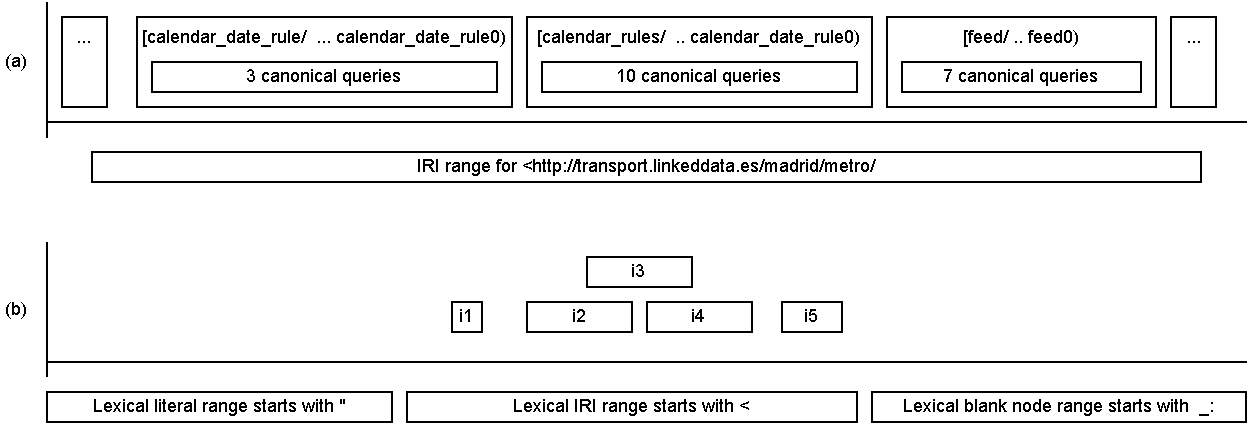
\includegraphics[width=0.95\textwidth]{images/range-partitioning.pdf}
%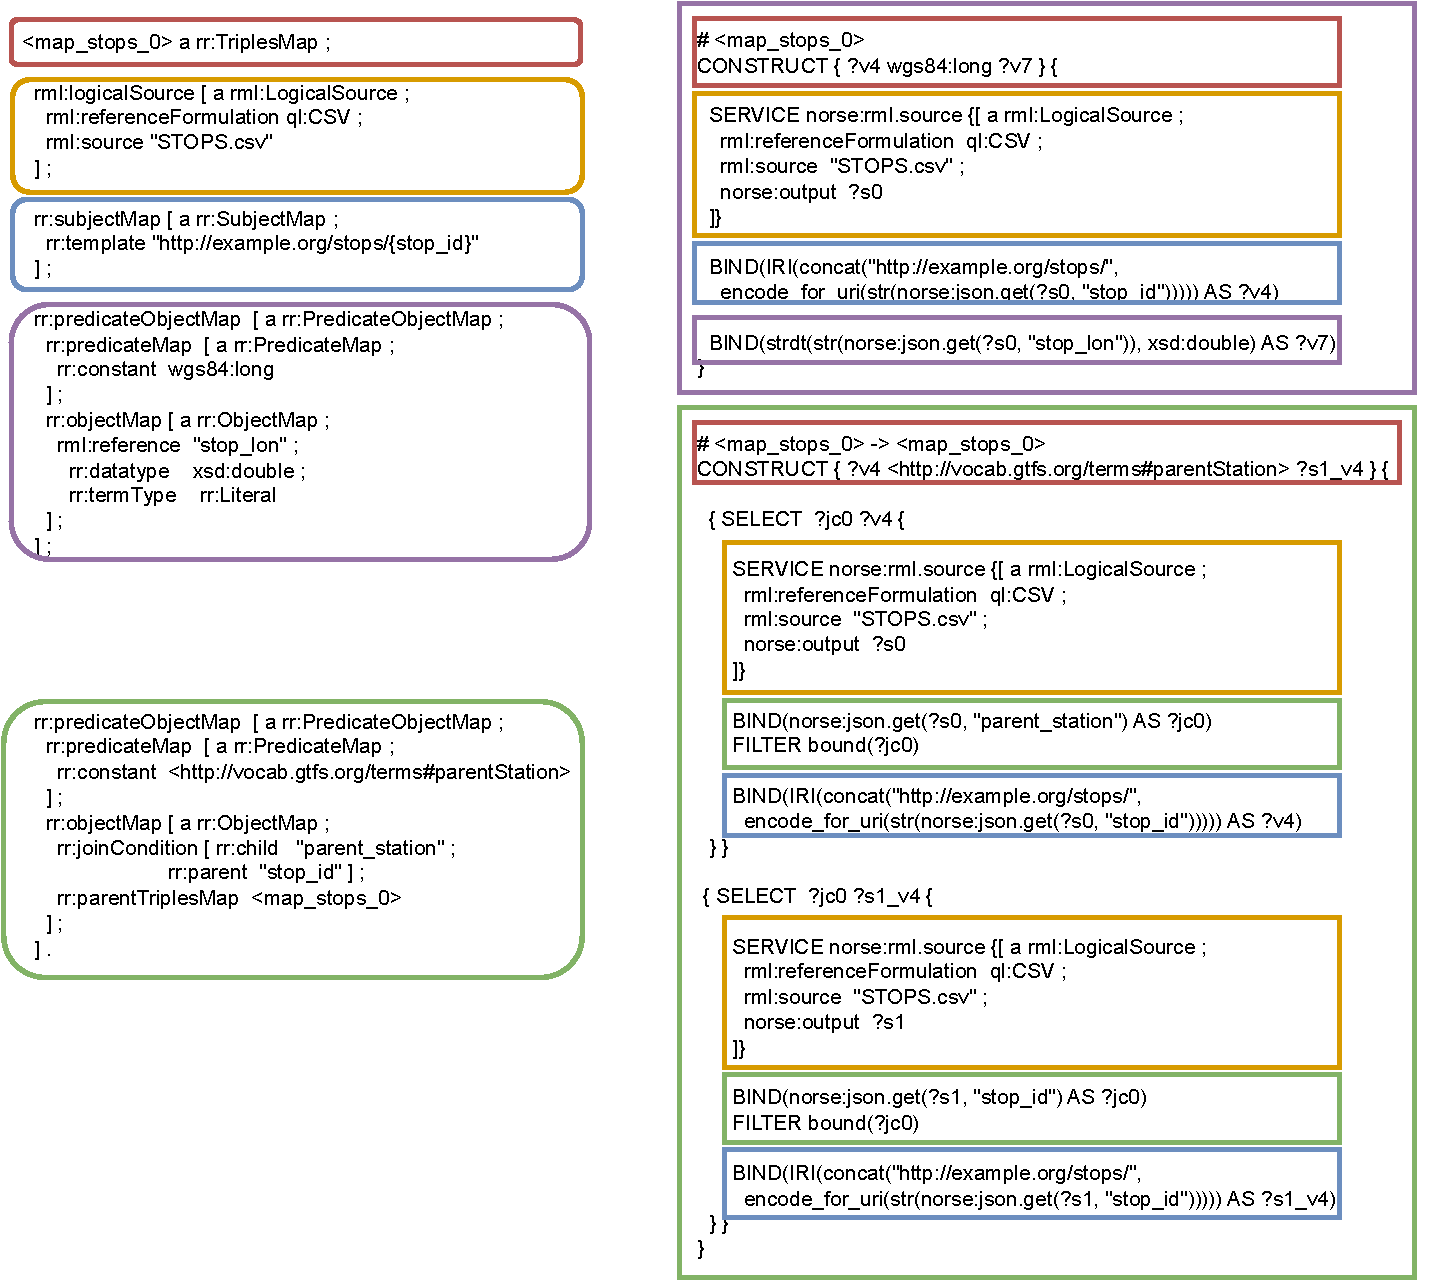
\includepdf[pages=-]{images/rml-to-sparql.pdf}

\caption{(a) An excerpt of the concrete range partitioning of canonical queries obtained from the GTFS-Madrid-Bench mapping based on their produced subjects. (b) An abstract model for RDF Term serialization in N-Quads with example intervals of which some (i3, i4, i5) overlap.}
\label{fig:range-partitioning}
%\caption{Execution time of partitioned queries using SANSA Query 0.9.0 vs Morph KGC 2.4.0}
\end{figure*}


\begin{figure*}[!h]
 \begin{minipage}[t]{0.29\textwidth}
  \centering
  \begin{lstlisting}[language=SPARQL, mathescape=true]
# Query $a$
CONSTRUCT {
  $s_{a_1}$ $p_{a_1}$ $o_{a_1}$
  ...
  $s_{a_n}$ $p_{a_n}$ $o_{a_n}$
} WHERE { $\mathrm{PATTERN_a}$ }

# Query $b$
CONSTRUCT {
  $s_{b_1}$ $p_{b_1}$ $o_{b_1}$
  ...
  $s_{b_m}$ $p_{b_m}$ $o_{b_m}$
} WHERE { $\mathrm{PATTERN_b}$ }
  \end{lstlisting}
%  \caption{listing}{Sub caption}
 \end{minipage}
 \begin{minipage}[t]{0.69\textwidth}
  \centering
  \begin{lstlisting}[language=SPARQL, mathescape=true]
CONSTRUCT { ?s ?p ?o }
WHERE {
  SELECT DISTINCT ?s ?p ?o {
      { $\mathrm{PATTERN}_a$
        LATERAL { { BIND($s_{a_i}, p_{a_i}, o_{a_i}$ AS
          ?s, ?p, ?o) } UNION ... } } # for i in 1..n
    UNION
      { $\mathrm{PATTERN}_b$
        LATERAL { { BIND($s_{b_j}, p_{b_j}, o_{b_j}$ AS
          ?s, ?p, ?o) } UNION ... } } # for j in 1..m
  } ORDER BY ?s ?p ?o
}
  \end{lstlisting}
  %| i \in \{ 1, \ldots, n \}$ 
%  \caption{listing}{Another sub caption}
 \end{minipage}
 \vspace*{-5mm}
 \caption{Generic merge of two (triple-based) CONSTRUCT queries into a single one based on their LATERAL form. The use of DISTINCT and ORDER BY is exemplary to demonstrate the production of truly unique and ordered "inter-query" tuples.}
\label{fig:combine-lateral}
\end{figure*}

%Intutively, it extends SPARQL with support for mapping a single binding to a set of bindings by parameterizing a graph pattern with it. ''flat-Map`` operations 

\subsection{Partitioning Mappings}
In~\Cref{sec:rml-to-sparql} we showed how to translate RML TriplesMaps into a set of SPARQL CONSTRUCT queries. Furthermore, we described how a set of CONSTRUCT queries can be combined into a single one using the novel \texttt{LATERAL} keyword.
This tooling is already sufficient to produce a single CONSTRUCT query from any RML document where DISTINCT and ORDER BY is applied at the top of its SPARQL algebra expression.
However, if it is known that two queries produce disjoint sets of RDF tuples then DISTINCT (and possibly ORDER BY) can be applied independently and their results can be UNION'd. As this leads to operations on fewer data it can significantly improve performance.

In order to achieve this goal it is necessary to obtain a description of the possible set of RDF tuples that can be created from a CONSTRUCT query.
For this purpose we introduce a  model where the set(s) of possible RDF terms (produced by a tuple's component) are represented as intervals.
%Akin to a number line, our interv
%n interval-based
%on a generalized number line.
%It is noteworthy, that the mobindings of a SPARQL result and how to order lines of an N-Quads serialization.
For brevity, we only focus on sorting RDF terms based on the lexical space of their N-Quads serialization.

For example, from an expression such as \lstinline{BIND(IRI(CONCAT("gtfsbench/", ?id)) AS ?x)} we can derive that \texttt{?x} may be any of (1) \texttt{unbound}\footnote{This is the case if \texttt{?id} is not a string because CONCAT only allows for string arguments.} or (2) an IRI with a string value in the interval $[\mathrm{"gtfsbench/"}\; .. \; \mathrm{"gtfsbench0")}$ (under lexicographic order), where $[$ denotes a closed boundary and $)$ an open one, and ``0'' is the successor character of ``/'' in (the ASCII-subset of) UTF-8.

Given a tuple of a construct template, we can thus determine a set of possible values for each of its components.
If the construct template has multiple quads then we can take the component-wise union of the intervals in order to obtain a single description of its producible quads.
% Mention SPAN - so 1 query - 1 interval!
If a variable's set of values is unknown we can gracefully represent it as an interval covering the complete range such as $({-\infty}\; .. \; {+\infty})$.
This way, we can ''project`` every CONSTRUCT query to an interval. \Cref{fig:range-partitioning}~(a) shows a concrete projection based on a subset of the mappings of the GTFS-Madrid-Bench. Each interval corresponds to one or more CONSTRUCT queries.
\Cref{fig:range-partitioning}~(b) shows an abstract example where intervals overlap.
A set of queries with overlapping ranges forms a \emph{partition} and can be merged as shown in~\Cref{fig:combine-lateral} for the sake of applying DISTINCT and ORDER BY.
%\todo{We need to say that we can cluster the CONSTRUCT queries by their interval and then merge them with DISTINCT and ORDER BY applied as described earlier}
Extending this approach to SPARQL is possible but more complex because then the definition of intervals need to consider of the RDF term types and RDF literal datatypes.
%segmentation of the ``number line'' into sub-intervals for each RDF term type and RDF literal datatype.

\subsection{Optimizing DISTINCT by Pulling Up BINDs}
A short-coming of the generated queries is that the DISTINCT operation runs over variables that may be assigned to constants.
By ``pulling'' such definitions up in the algebra DISTINCT can operate on significantly fewer data, which in general increases performance by means of lowering the computational overhead. \Cref{fig:pull-extend} shows an example of rewrite rules we use for optimization. Note, that \texttt{EXTEND} is the algebraic correspondence to the \texttt{BIND} syntax\footnote{\url{https://www.w3.org/TR/sparql11-query/\#sparqlAlgebra}}.
Note, that more sophisticated rules can be devised to split expressions such as \lstinline{CONCAT(const, ...)} into a constant and variable part where the constant part can be pulled up.

%The following algebraic transformation rules allow for "pulling" constant assignments over \texttt{DISTINCT} operations:
%Common variable expression list (commonVel) must be a mapping of variables to constants.
\begin{figure*}[!h]
\begin{itemize}
    \setlength\itemsep{-0.5em}
%    \item Pulling constant assignments up over distinct \texttt{DISTINCT}:
    \item \lstinline{DISTINCT(EXTEND(var, constant, subOp))} $\rightarrow$ \lstinline{EXTEND(var, constant, DISTINCT(subOp))}
    \item \lstinline{UNION(EXTEND(var, constant, left), EXTEND(var, constant, right))} $\rightarrow$
    
    \hspace{1cm}\lstinline{EXTEND(var, constant, UNION(left, right))}
    \item \lstinline{EXTEND(var, non-constant-expr, EXTEND(var, constant, subOp))} $\rightarrow$
    
    \hspace{1cm}\lstinline{EXTEND(var, constant, EXTEND(var, non-constant-expr, subOp))}
\end{itemize}
\vspace*{-5mm}
\caption{A brief excerpt of algebra rewrite rules used to pull EXTEND up.}
\label{fig:pull-extend}
\end{figure*}

\section{Implementation}
\label{sec:implementation}
In this section we provide a brief overview of our related implementations: The NORSE Sparql Extensions, the implementation of the SANSA binding engine (SaBiNe) for evaluating SPARQL on Apache Spark, and finally the RDF Processing Toolking \emph{RPT} which bundles all components together -- including the RML to SPARQL tooling -- into a single command line toolkit.

\paragraph{NORSE SPARQL Extensions and RPT}
JenaX is our project of unofficial extensions for the Apache Jena project. Among its features are the \emph{NORSE} SPARQL extensions. Adding the plugin module as a Maven dependency enhances a Jena-based project with the datatypes and functions for processing CSV, XML and JSON\footnote{\url{https://mvnrepository.com/artifact/org.aksw.jenax/jenax-arq-plugins-bundle}}.

%Committede to upstreaming stable features to Jena or conversely, upstreaming enhancements in order 
\paragraph{Evaluating SPARQL with SANSA and Apache Spark}
Our approach to evaluating SPARQL in Spark is a direct one: A SPARQL result set is represented as an \lstinline{RDD<Binding>}.
%Furthermore, let $\mathrm{Op}$ be the set of SPARQL algebra expressions.
On this basis we present a translation function $[[.]]$ that recursively translates SPARQL algebra operations to operations on (Java) RDDs.
The SANSA Framework thereby provides several features that enable use of functionality from Apache Jena with Apache Spark, such as serializers for SPARQL bindings and algebra expressions. \Cref{lst:sparql-to-spark} shows an excerpt for the evaluation of the SPARQL operations most relevant to RML execution on Apache Spark .

\begin{figure*}[htb]
\begin{itemize}
\setlength\itemsep{-0.5em}
\item \begin{lstlisting}[mathescape=true]
$[[$SERVICE norse:rml.source {[ ... norse:output ?s ]}$]]$ := Create a RDD<Binding> where ?s is bound to records of the specified RML source.
\end{lstlisting}

\item \begin{lstlisting}[mathescape=true]
$[[$FILTER(subOp, expr)$]]$ := $[[$subOp$]]$.filter($\mu \rightarrow \mathrm{exprEval}(\mathrm{expr}, \mu) == true$)
\end{lstlisting}

\item \begin{lstlisting}[mathescape=true]
$[[$JOIN(left, right)$]]$ := $[[$left$]]$.mapToPair($\mu_1 \rightarrow \langle \Pi_J(\mu_1), \mu_1 \rangle$).join($[[$right$]]$.mapToPair($\mu_2 \rightarrow \langle \Pi_J(\mu_2), \mu_2 \rangle$)).map($\langle \mathrm{key}, \langle \mu_1, \mu_2 \rangle \rangle \rightarrow \mu_1 \cup \mu_2$)
\end{lstlisting}
where $J$ is the set of join variables $\mathrm{vars}(\mathrm{left}) \cap \mathrm{vars}(\mathrm{right})$ and $\Pi_J(\mu)$ is the projection of a binding to these variables.
%.filter($(\mu_1, \mu_2) \rightarrow \mathrm{isCompatible}(\mu_1, \mu_2)$)
%and $\mathrm{joinKey}$ is a function that maps each binding to a 
%$\mathrm{vars}(\mathrm{left}) \cap \mathrm{vars}(\mathrm{right})$

\item \begin{lstlisting}[mathescape=true]
$[[$PROJECT(subOp, vars)$]]$ := $[[$subOp$]]$.map($\mu \rightarrow \Pi_{vars}(\mu)$)
\end{lstlisting}

\item \begin{lstlisting}[mathescape=true]
$[[$DISTINCT(subOp)$]]$ := $[[$subOp$]]$.distinct()
\end{lstlisting}

\item \begin{lstlisting}[mathescape=true]
$[[$LATERAL(left, right)$]]$ := if right has no basic graph patterns then
    $[[$left$]]$.mapPartitions($\mu \rightarrow \{ \mu \cup \nu | \forall \nu \in \mathrm{convEval}(\mathrm{subst}(\mathrm{right}, \mu)) \}$)
\end{lstlisting}
where $\mathrm{convEval}$ is conventional SPARQL evaluation into a (Java) collection of bindings rather than a Spark RDD.

\item \begin{lstlisting}[mathescape=true]
$[[$EXTEND(var, expr, subOp)$]]$ := $[[$subOp$]]$.map($\mu \rightarrow \mu \cup \{ \mathrm{var} \rightarrow \mathrm{exprEval}(expr, \mu) \}$)
\end{lstlisting}
\end{itemize}
\vspace*{-5mm}
\caption{Evaluation of selected SPARQL operations with Apache Spark}
\label{lst:sparql-to-spark} 
\end{figure*}

% Issue: The RML sources  actually require this additional project https://github.com/Scaseco/r2rml-api-jena
\paragraph{RDF Processing Toolkit} RPT is the integration project that provides a powerful frontend for both Jena's ARQ and SANSA's SPARQL engines. Both engines support the NORSE and the RML extensions, however only the latter supports parallelization. Example usage of the tooling is shown in~\Cref{lst:usage}.
%and easy-to-use

%# RML to SPARQL Translation
%# Execution
% basicstyle=\scriptsize
\begin{lstlisting}[label=lst:usage, basicstyle=\footnotesize, caption=Example for using RPT to translate and execute RML]
rpt rmltk rml to sparql mapping.rml.ttl > raw.rq
rpt rmltk optimize workload raw.rq --no-order > mapping.rq
JAVA_OPTS="-Xmx16g" rpt integrate mapping.rq --out-file rpt-arq.nt
JAVA_OPTS="-Xmx16g" rpt sansa query mapping.rq --out-file rpt-sansa.nt
\end{lstlisting}


\section{Evaluation}
\label{sec:eval}
We evaluate our approach on the GTFS-Madrid-Bench and one of the largest datasets of SDM-Genomics-Datasets\footnote{The used files are 75percent\_of\_records\_with\_duplicate\_and\_each\_duplicate\_being\_repeated\_20times.csv and 4POM\_Normal.ttl}.
For this purpose we converted the benchmark's RML files to extended SPARQL and ran them using Jena's ARQ and SANSA's SPARQL engine as shown in~\Cref{lst:usage}.
In a first step we evaluated several RML tools on a server with 128GB RAM, AMD Ryzen 9 5950X 16-Core CPU and SSD storage running Ubuntu 20.04.
In order to establish comparability, we used all tools' native unique output feature\footnote{The only exception was Carml for which we appended a \texttt{sort -u} step}. The results for the scale factors 1, 10, 100, 300 are shown in~\Cref{fig:tool-comparison}.
We also attempted to evaluate RocketRML, however we ran into memory issues with it\footnote{\url{https://github.com/semantifyit/RocketRML/issues/44}}.
As for \emph{RMLStreamer}\cite{Haesendonck2019}, on the one hand it requires a Flink setup and on the other hand the initially obtained execution suggested that it lacks the self-join elimination - similar to RMLMapper.

\begin{figure*}[htb]
\centering
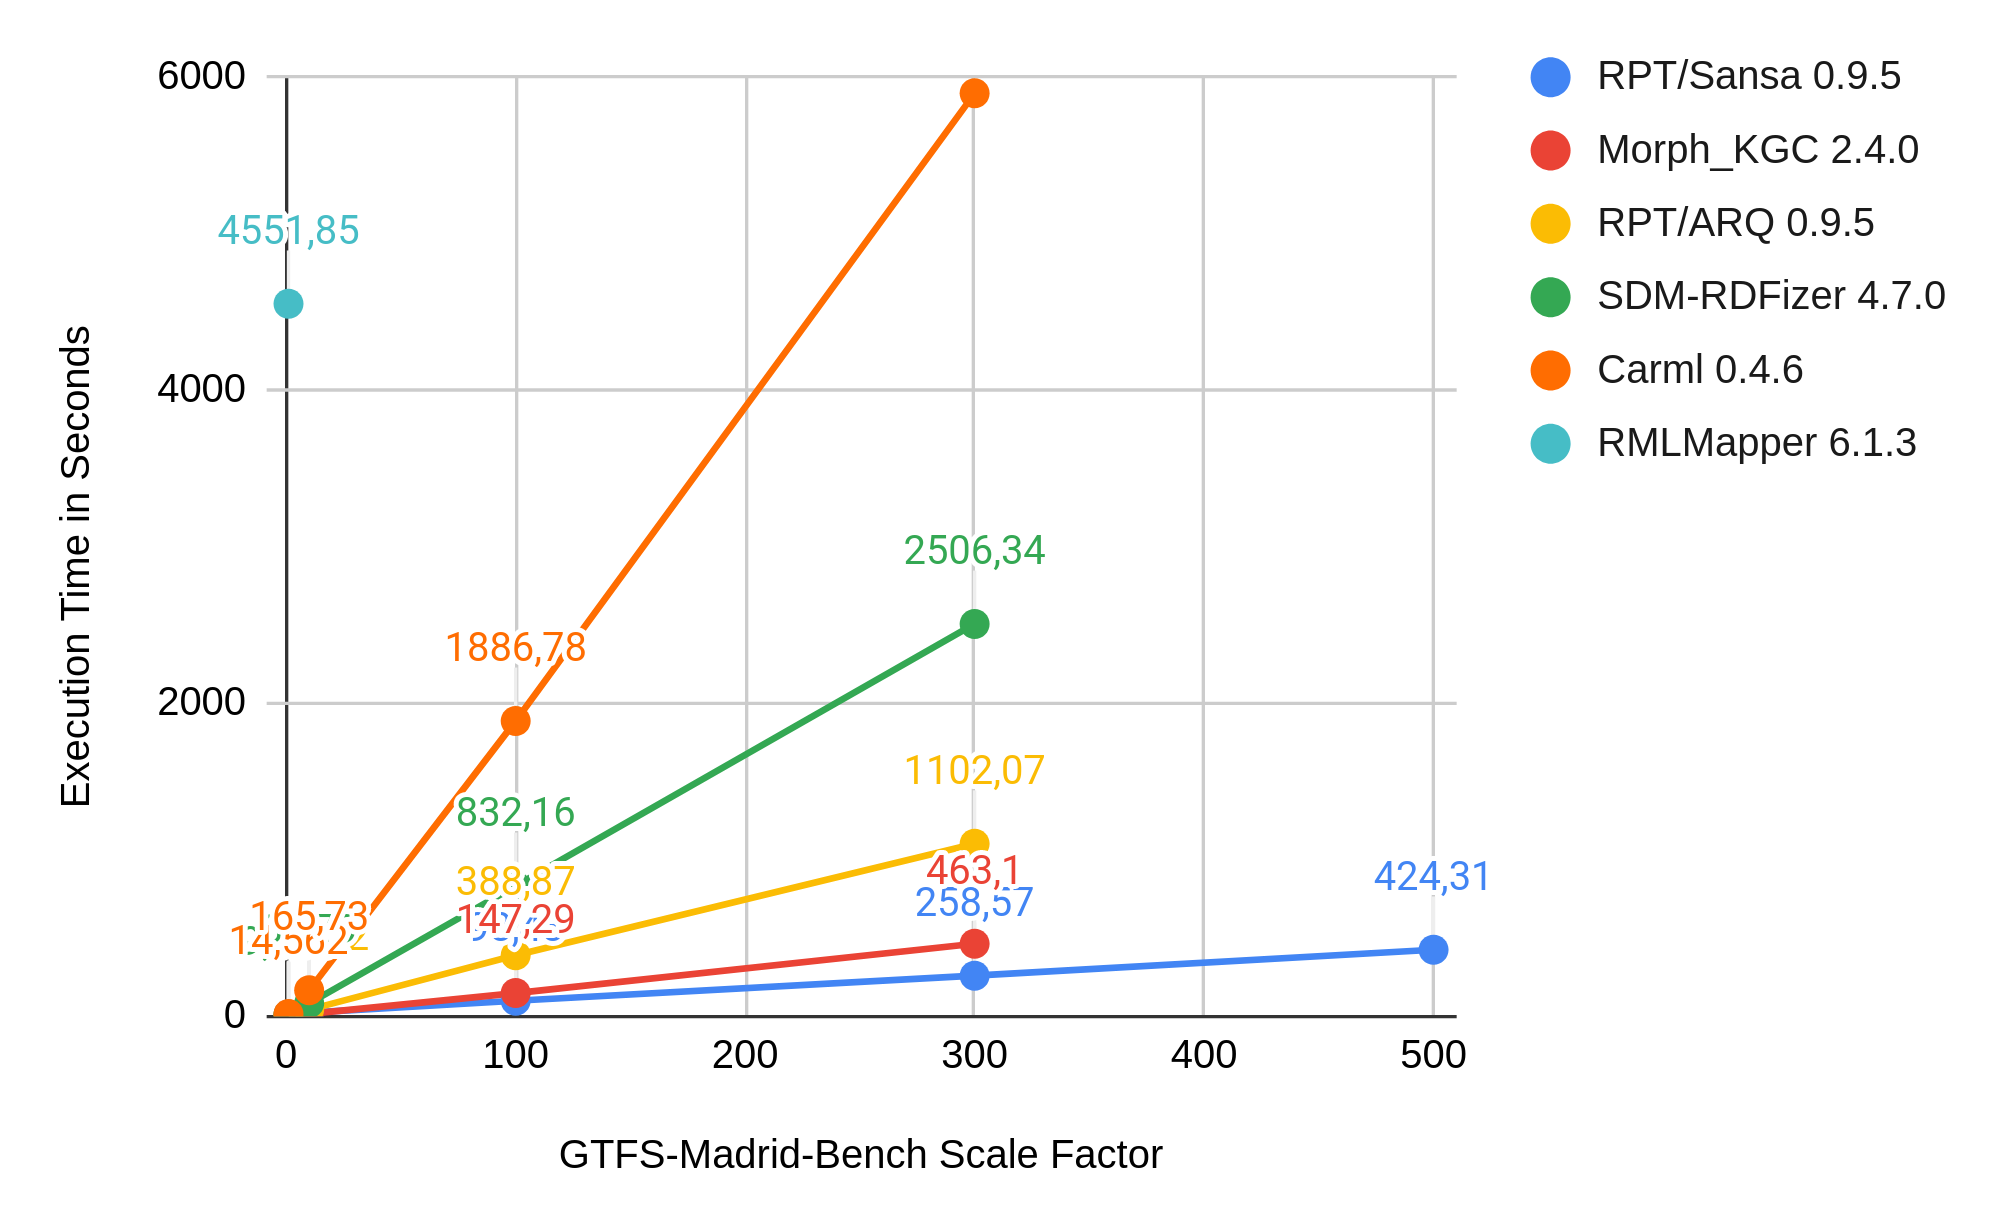
\includegraphics[width=0.7\textwidth]{images/rml-all-tools.png}
%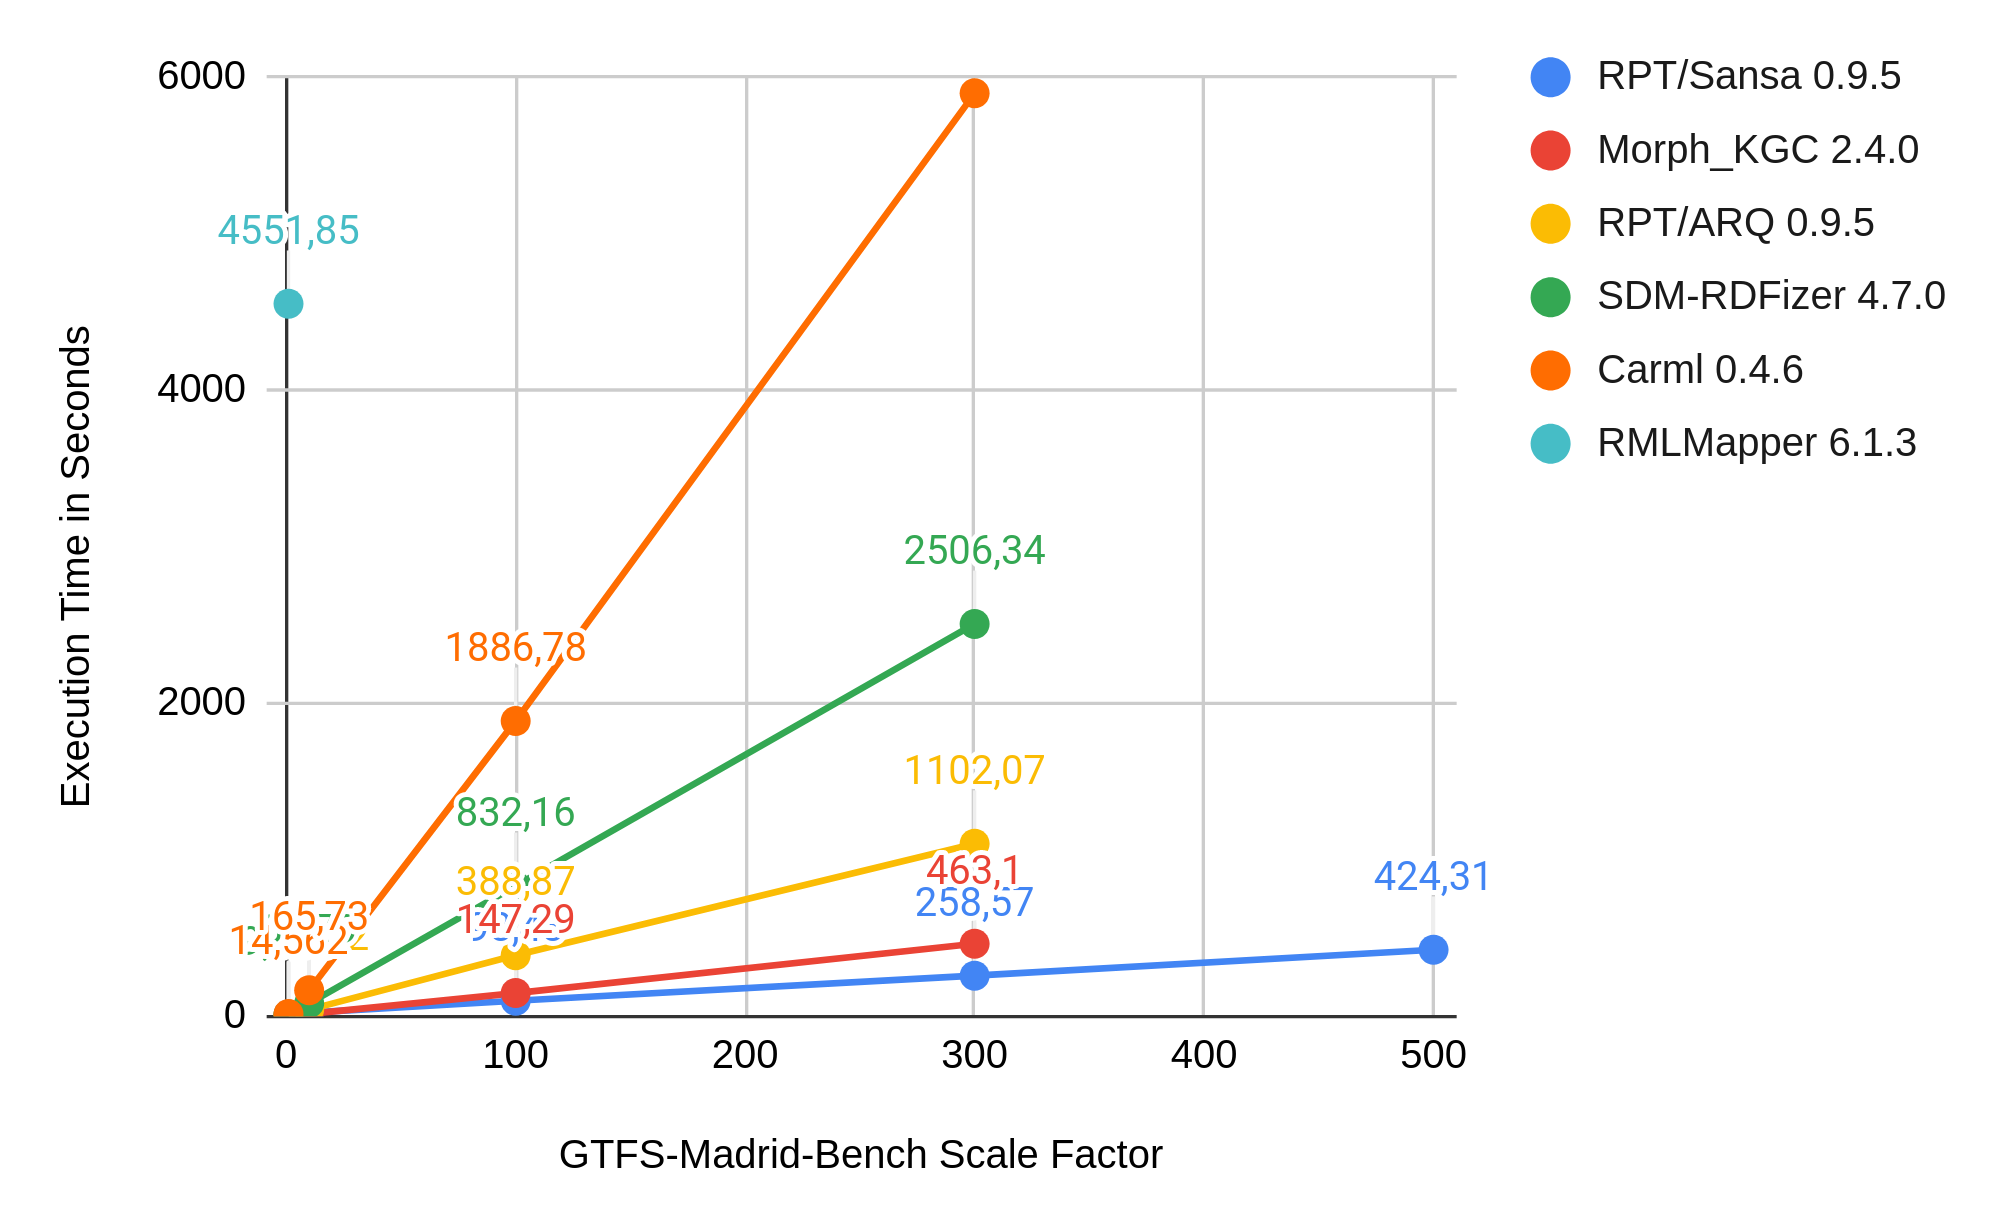
\includepdf[pages=-]{images/rml-all-tools.pdf}
\caption{Comparison of RML mapping tool performance with 128G RAM. On scale factor 500, RPT/ARQ and Morph\_KGC ran out of memory. Carml and SDM-RDFizer were already a magnitude slower on scale factor 300 and were not further evaluated. RMLmapper already exhibited a very high execution time on scale factor 1.}
\label{fig:tool-comparison}
\end{figure*}

In a subsequent step, we evaluated the fastest approaches which are the ones that rely on parallel processing, namely \emph{Morph\_KGC} and \emph{RPT/SANSA}.
%In order to rule out I/O boundness
For this evaluation we needed a machine with more RAM and its specs were: Ubuntu 22.04, 2x Intel(R) Xeon(R) CPU E5-2683 v4 @ 2.10GHz (totalling to 64 threads) and 512GB DDR4 RAM at 2133 MHz. In order to avoid I/O bounds in parallel processing, we performed the experiments for both tools with the benchmark datasets served from the default RAM drive \texttt{/dev/shm}.
With this machine it was possible to scale up to factor 1000.
In addition, we evaluated the tools on the SDM-Genomic-Dataset as this includes a workload that does not involve joins but many duplicates.
As can be seen from~\Cref{fig:eval-chart-execution-time} the execution times for both tools on both workloads converge to scaling linearly.
On smaller sizes Morph\_KGC outperforms RPT/SANSA. With increasing data scale the Apache Spark-based approach gains an advantage. However, on the workload that is mainly about duplicate removal the performance benefit is quite small considering CPU usage:
Morph's average CPU usage in both scenarios is roughly around 400\% whereas RPT/SANSA's is around 4000\%. This means that the latter requires almost 10 times the CPU resources of the former in order to accomplish the same task.
There are many aspects that can cause this significant difference: As a primary source we suspect Apache Spark's processing model for DISTINCT which relies on hash partitioning and shuffling of data which involves (de-)serialization. This introduces a significant overhead when compared to e.g. simply keeping records in an in-memory hash set. Also, Jena introduces additional overhead by having to parse all RDF literals for expression evaluation. 
The benefit is, that invalid literals are reported whenever they are produced during knowledge graph construction.
A performance issue which we detected and fixed during profiling was that Jena would needlessly materialize literals during SPARQL evaluation\footnote{\url{https://github.com/apache/jena/pull/1802}}. Overall, further investigations are necessary to assess the impact of all relevant aspects on the performance in detail.
%the differences in performance in detail.
%substantiate the explanations of the differences.
%This is needed for the evaluation of SPARQL expressions.
%Furthermore, building on an existing SPARQL engine can be both a blessing and a curse: In contrast to Morph\_KGC's current implementation, Jena introduces additional overhead by validating and parsing RDF literals warns about invalid ones.
%. which introduces representations and warns about invalid ones.
%Thereby invalid literals, which occur in the GTFS-Madrid-Bench, further negatively impact performance due to raising internal exceptions.


\begin{figure}
    \centering
    \subfloat[\centering]{{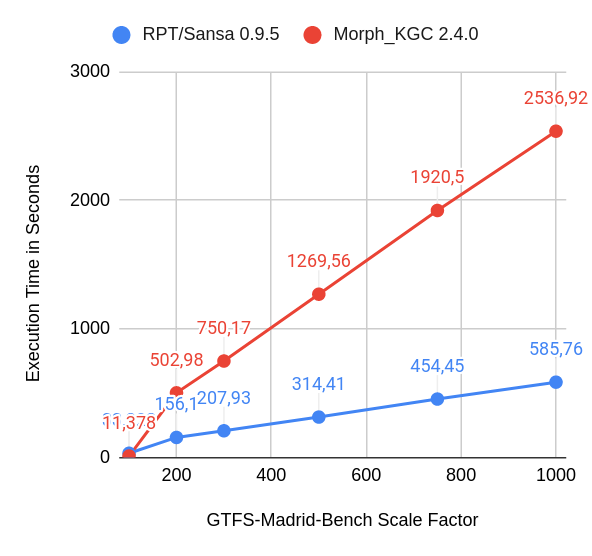
\includegraphics[width=0.47\textwidth]{images/rml-gtfsbench-sansa-vs-morph.png} }}
    \qquad
    \subfloat[\centering]{{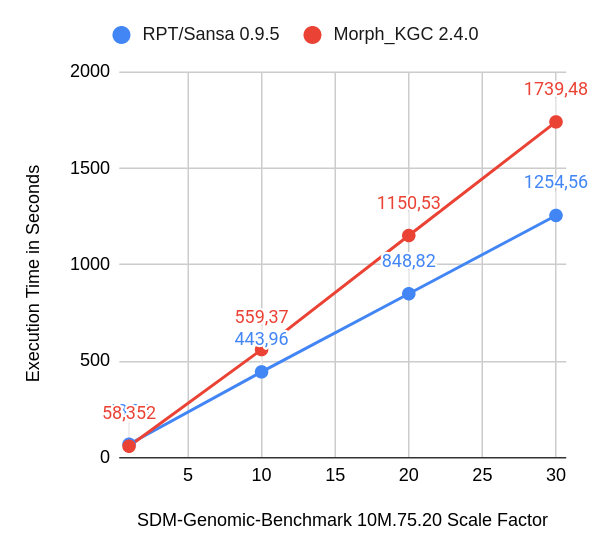
\includegraphics[width=0.47\textwidth]{images/rml-sdm-genomic-morph-vs-sansa.png} }}
    \caption{Execution time of RPT/SANSA and Morph\_KGC with 512G RAM and all data (including temporary) in a RAM disk.}
    \label{fig:eval-chart-execution-time}
\end{figure}


\section{Conclusions and Future Work}
\label{sec:conclusions}
In this work we showed that with the conversion of RML to SPARQL we can leverage suitably enhanced SPARQL engines for the task of knowledge graph construction.
%Just like YARRRML can be converted to RML,  a common ground for query and workload optimization.
We further showed that by transforming CONSTRUCT queries to their ``lateral'' form it is now finally possible to ``merge'' CONSTRUCT queries and remove duplicates which has direct applications in knowledge graph construction.
%Furthermore, using a simple join analysis we can optimize JOINs on Spark by transforming expensive hash joins into cheaper broadcast joins.
Using query workload analysis we can push down DISTINCT operations such that this expensive operation can be computed on smaller RDF graphs.
We showed that the same query workload can be executed on different engines yielding the same result sets however with significantly different performance characteristics. By leveraging a Big Data framework this approach can outperform state of the art approaches.
%In particular, to the best of our knowledge, our Big Data-based approach is the first one to scale to the GTFS1000 benchmark.
We emphasize that as part of this work we contributed the SERVICE extension plugin system as well as minor performance improvements
%as an initial LATERAL implementation
to Apache Jena.
%Our contribution was picked up in Oxigraph and sparked standardization efforts for SPARQL 1.2.
One direction of future work is to optimize the generated SPARQL algebra further as to minimize the amount of data that has to be processed in DISTINCT and ORDER BY operations. Also, as shown in the evaluation, the improved overall performance comes at the cost of significant higher resource usage for which we plan in-depth investigation of the reasons and possible mitigation approaches such as using custom Spark operator implementations.
Furthermore, we identify the need for the standardization of SPARQL for heterogeneous data as this would not only make it possible to transform RML to SPARQL in a truly interoperable way, but also provide a common ground for query and query workload optimization.

%%
%% Define the bibliography file to be used
%\bibliography{ref}




% Exploration

\section{Introduction}
Faceted browsing is ubiquitous on the Web today. Most if not all major online shops and media (video, images and music) platforms provide at least some degree of faceted browsing features to
navigate their products - or more specifically: the data records about them. Typical examples include support for filtering videos by length, music by genre, or generally products by relevant features[
%as shown in \autoref{fig:faceted-browsing-demo}. 
Conceptually, in many cases the underlying data can be seen as knowledge graphs (KG), i.e. entities and values are represented as nodes, and labelled edges are used to specify their semantic relation. In cases where data is modelled using RDF (and ontologies), it already forms a knowledge graph. In this case, SPARQL\footnote{\url{https://www.w3.org/TR/sparql11-query/}} is a standard language for uniformly querying instance and schema information.

In this paper, we present our SPARQL-based faceted browsing benchmark generation framework, designed to generate realistic faceted browsing scenarios on arbitrary data sets and assess triple store performance in regard to the faceted browsing paradigm.
%\todo{set-theoretic approach}
%Motivation
%- several faceted browsing systems
%  focus on user interfaces
%  - or generic benchmark with focus on triple store performance
%  - but with these approaches, to what extend user exploration via sparql works remains a mystery.
%- most if not all benchmarks require specific data sets - hard to evaluate one's own use case

Our contributions are as follows:
\begin{itemize}
    \item A highly flexible, schema-agnostic SPARQL-based faceted browsing benchmark generation framework
    \item Configurable benchmark generation based on chokepoints and user-provided data sets
%    \item Investigation of current limitations of real-time SPARQL-based faceted browsing
%    \item Evaluation of the schema-based path finding component used in benchmark generation
    \item Performance and correctness evaluation of contemporary triple stores using the HOBBIT benchmarking platform
\end{itemize}

Our resource is available at \\ \url{https://github.com/hobbit-project/faceted-browsing-benchmark}.

The remainder of the paper is structured as follows:
In~\autoref{sec:preliminaries}, we introduce the RDF and SPARQL and on this basis define the important notions.
Afterwards, in ~\autoref{sec:architecture}, we present the overall architecture of our system. The main building blocks are the faceted search query generation system and a component for schema-based path finding along properties, which are described in~\autoref{sec:engine}.
The benchmark generator itself is presented in~\autoref{sec:benchmark-generator}.
Our findings are reported on in~\autoref{sec:evaluation}.
We discuss related work in~\autoref{sec:related-work}. Finally, we conclude in~\autoref{sec:conclusions} and where we also point out directions for future work.

%\subsection{Resources}
%- Links to all resources:
%- Benchmark Generator
%- Generated Benchmarks
%- Hobbit Platform

%\section{Preliminaries}
%RDF, SPARQL, BGP

%In~\autoref{sec:engine} we present our SPARQL-based faceted search %engine, which is a fundamental building block of benchmark %generation system.

\section{Preliminaries}
\label{sec:preliminaries}
%The engine is data-driven, which means that facets and facet values correspond directly to the available properties and property values, respectively, in an RDF dataset.

\subsection{RDF and SPARQL}
The Resource Description Framework (RDF) is a W3C standard for data interchange\footnote{\url{https://www.w3.org/RDF/}}.
The most fundamental introduced entity is the \emph{RDF graph} which conceptually is a set of triples.
A triple can be seen as a labelled ``link'' between two nodes.

Formally, let there be sets of IRIs $I$, blank nodes $B$ and literals $L$. Further, let the set of
\emph{RDF term}s $T := I \cup B \cup L$.
An \emph{RDF Graph} $G$ is defined as $G \subset (I \cup B) \times I \times T$.

Although RDF graphs are often depicted as conventional labelled graphs, they are formally defined of ternary relations which in turn correspond to directed labelled pseudo graphs. Pseudo graphs allow for multiple edges
to exist between a given pair of nodes, as well as for the same node to act as the start and end of an edge.
Hence, in some cases commonly used graph algorithms may not be applicable to given RDF data.
% Vocabularies

SPARQL (a recursive acronym for \emph{SPARQL Protocol and RDF Query Language})
is a W3C standard that devises protocols and languages for querying and updating RDF.
Our benchmark generator will produce SPARQL queries that correspond to faceted search and browsing operations on an RDF data set. The generated benchmarks can be executed on any system implementing SPARQL.
% Graph pattern
%Triple stores


\subsection{Paths}
With SPARQL 1.1, \emph{property paths} expressions were introduced to the query language.
Since then it is possible to query a data set for all pairs of resources connected via sequences of RDF predicates that match a given path expression. For instance, \emph{?sub rdfs:subClassOf* ?super}
will yield any pair of resources reachable by zero-or-more forward traversals along the \emph{rdfs:subClassOf} predicate.
For our work, we introduce the notion of \emph{simple (property) paths} as (possible empty) sequences of \emph{steps} which are (predicate, direction) pairs. Direction is either \emph{forwards} or \emph{backwards}.


%Further, we introduce the following notions, which in the case of empty paths all yield \emph{nil}.
%\begin{itemize}
%  \item $parent(path)$ yields the parent path (i.e. the path with the last step omitted).
%  \item $reachingPredicate: P \rightarrow I$ yields the (predicate) IRI by which the path's destination is reached, i.e. the last predicate of a path.
%  \item $reachingDirection: P \rightarrow D$ analogously yields the direction of the last step.
%\end{itemize}

%We introduce the notion of an \emph{arrow} as a pair combining a path with direction.\footnote{One can think of the path
%acting as the shaft, and the direction as the tip.}

\subsection{Node-centric Sparql Queries}
\begin{lstlisting}[language=sparql, label=lst:pquery, caption=Pseudo code for a node-centric query and property access]
NodeCentricQuery
  .from(
      CONSTRUCT WHERE {
          ?employee :employedAt ?department ;
                rdfs:label ?l 
      })
  .partitionBy(?employee)
  .executeOn(sparqlEndpoint)
  .forEach(rdfNode -> rdfNode.getProperty(rdfs:label))
\end{lstlisting}
\emph{CONSTRUCT} is a standard SPARQL query form which allows for retrieval of RDF graphs. However, many use cases do not demand for a single monolithic RDF graph,
but rather individual partitions that form logical objects that can be processed independently.
For example, a query about employees and departments may look like \autoref{lst:pquery}.
From the query alone, one cannot deduce whether it is department-, employee- or triple-centric.
However, if we denoted e.g. \emph{?department} as a \emph{partition} variable, we can easily group triples
based on this condition for further processing.
A \emph{node-centric SPARQL query} is thus simply a pair comprised of a standard construct query and a single partition variable.
Partitioning could also be applied to \emph{SELECT} queries, however, in the case of \emph{CONSTRUCT}, access of retrieved data becomes object-like. %, and thus exhibits benefits:
%Similar to as one would access properties of e.g. a JSON object, one can -- starting from a binding of one of the partition variables %--
%access its retrieved predicates, as sketched in~\autoref{lst:pquery}.
Note, that the construct template may be empty, in which case the result is a set of RDF terms (such as literals) with no related triples.
% aspect is, whether to treat each instance of the CONSTRUCT template as an object, or 
%In fact, the Apache Jena framework\footnote{\url{https://jena.apache.org/}} features tooling to 

In our work, we use this mechanism for obtaining facet values and counts.

\section{Framework Architecture}
\label{sec:architecture}

\begin{figure}
\centering
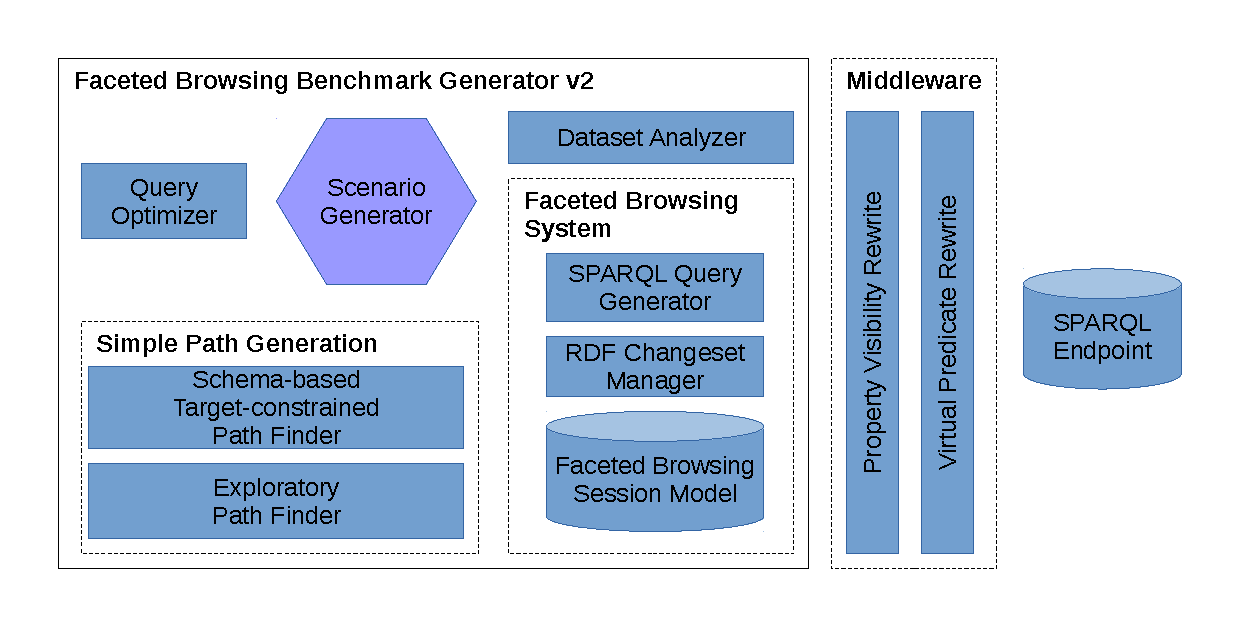
\includegraphics[width=\textwidth]{images/Architecture}
\caption{Architecture of the Schema-agnostic SPARQL-based Faceted Browsing Benchmark Generation\label{fig:architecture}}
\end{figure}

\autoref{fig:architecture} depicts the components of our faceted browsing benchmark generation system, which we briefly explain below: 
\begin{itemize}
\item The \emph{Scenario Generator} drives the benchmark generation and uses the APIs and services provided by the other components.
A scenario is a sequence of faceted browsing interactions.
\item The \emph{Dataset Analyzer}'s purpose is to obtain metadata about a data set. Most relevant to us are the used predicates and their ranges, and the schema-graph, i.e. which instance types are connected by which properties.
%(see \autoref{sec:dataset-analysis}).
This metadata is used by the path finder sub-system.
\item The \emph{Exploratory Path Finder} tries to generate -- starting from a set of resources -- simple paths that meet given specifications.
\item The \emph{Schema-based Target-constrained Path Finder} is used to find simple paths that end in a given set of predicates, such as a numeric one or a pair that represents longitude and latitude. This component uses the schema-graph to generate candidate paths. %The system under test (SUT) SPARQL endpoint is then queried for whether there are actually resources connected by the candidate paths.
\item The \emph{Query Optimizer} is used to post-process generated SPARQL queries in order to make them more natural as if they were written by a human expert.
For instance, whenever possible, variables in triple patterns are substituted with constants and filter expressions are simplified. This has two purposes: On the one hand it relieves the work of query optimiser when testing the benchmark on target SPARQL systems.\footnote{Example issue that was mitigated by improving our own query optimiser: \\ \url{https://github.com/openlink/virtuoso-opensource/issues/822}}
\item The \emph{Middleware Layer} is the place where certain virtual data transformations relevant to faceted browsing can be implemented using query rewriting. (It is not part of the Benchmark Generator.) % Some triple stores support these rewriting features natively, whereas our framework provides limited triple-store-independent implementations.
%, whereas our framework also ships with prototype implementations. %integrated.
%we created prototype implementations which are summarized here for completeness:
%  \begin{itemize}
%  \item \emph{Property Visibility}: In many cases, it is undesired to have all predicates of a dataset to show up as facets in a faceted browser.
%  This component can hide predicates by means of injecting appropriate FILTER statements into SPARQL queries based on given whitelists or blacklists.
%  \item \emph{Virtual Predicate Rewrite}: Sometimes predicates desired to appear in a faceted browser are not directly present in a dataset.
  For example, browsing people by \emph{age} may feel more natural than by \emph{birth date}. In a data set, typically the latter predicate is preferred as it refers to static information, whereas the former one changes every year. This rewrite component allows one to define custom virtual predicates using SPARQL queries.    
%  \end{itemize}
\end{itemize}


\section{SPARQL-based Faceted Browsing System}
\label{sec:engine}
The most fundamental component of our benchmark system is unsurprisingly the faceted browsing system.
It provides the means necessary to interact with an RDF dataset according to the faceted browsing paradigm.
First, we present a domain-specific language for expressing faceted queries. Subsequently, we show how they are translated to SPARQL.
%The faceted browsing engine is one of the two core building blocks of HFBBG. 

\subsection{A domain-specific language for Faceted Search}
In this section, we present a domain-specific language (DSL) for the implementation of a faceted search system.
The main idea is as follows:

Given an intensional description of a set of resources, e.g. all subjects of an RDF graph or all instances of type person. We now need mechanisms to obtain information about them, navigate along their properties to related set of resources, and apply constraints on these sets. In principle, this corresponds to building a SPARQL basic graph pattern by starting with a \emph{root variable}, and adding appropriate connecting \emph{triple patterns} and \emph{filters} as query generation progresses.

The entry point to the system is the \emph{FacetedQuery}. It is modelled with the following parts:
\begin{itemize}
\item A \emph{base SPARQL concept} that denotes the initial set of resources. Typically it denotes all of an RDF graph's subjects, but
it could also be set to e.g. the instances of a certain class or the set of predicates.
\item A set of (facet) \emph{constraints} - We represent constraints as SPARQL expressions, however, with a level of indirection: Instead of using (final) variables directly, references to \emph{FacetNode} or \emph{FacetMultiNodes} (explained below) are used. In the query generation phase, these references are substituted with the corresponding variables.

%entities that represent traversals of the data.
%Essentially, these traversals are simple paths.
%These traversals entities are internally created when trav
%FacetNodes and FacetMultiNodes.
%The type of the traversal determines whether multiple constraints are to be combined using conjunctions or disjunctions.
\item The \emph{focus}
%is a designated \emph{FacetNode} that
denotes the set of resources that serve as the base for facet value counts computations, in other words the base of the resources on display.
%Note, that despite constraints being SPARQL expressions, they are not injected into final SPARQL query directly:
%One the one hand, every reference needs to be resolved to its final variable and graph pattern,
%On the other one, additional transformations may be required, such as converting a spatial constraint involving a bounding box into the appropriate vocabulary and/or SPARQL dialect, such as WGS84, GeoSPARQL or Virtuoso's flavor of it.
\end{itemize}

\begin{figure}
\centering
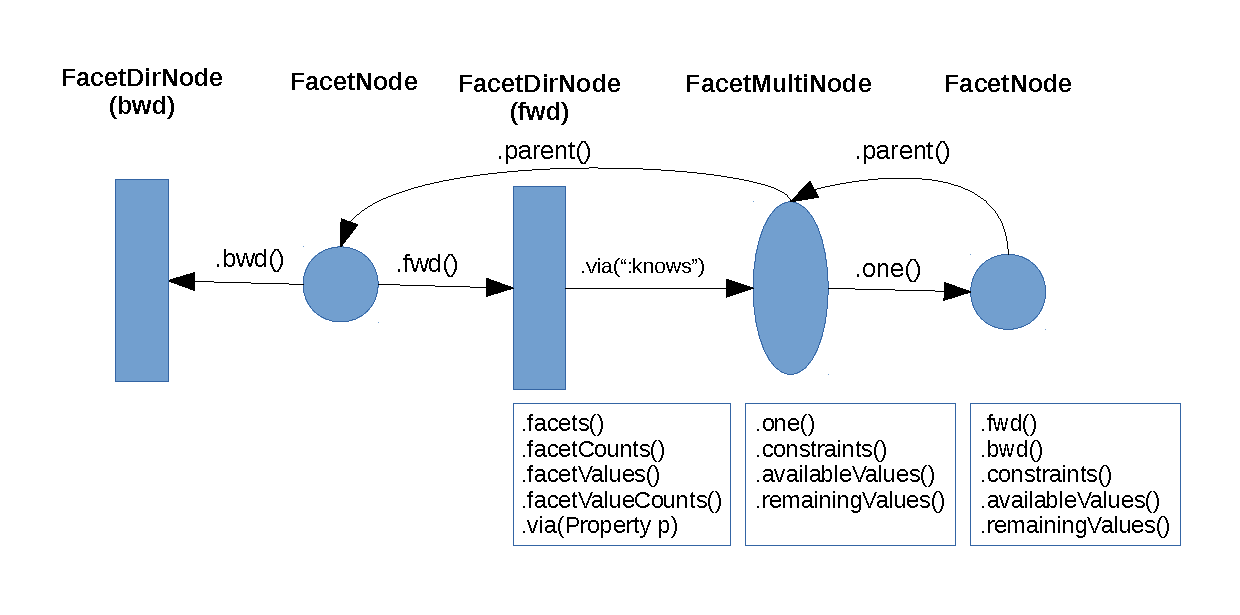
\includegraphics[width=\textwidth]{images/NodeModel}
\caption{The most relevant entity types and methods of the Faceted Browsing System. They enable traversal of a the data as well as retrieval of faceted-search-related information, such as available values or facet value counts.}
\label{fig:faceted-browsing-api}
\end{figure}
The focus of a FacetedQuery is a designated \emph{FacetNode}, whose related interfaces are depicted in~\autoref{fig:faceted-browsing-api} and are described as follows:
\begin{itemize}
\item A \emph{FacetNode} instance can be seen as a specific variable in a BGP  and thus intensionally represents a set of resources.
Using the \emph{.fwd()} or \emph{.bwd()} methods, one obtains a \emph{FacetDirNode} entity that represents the set of facets and facet values
reachable either in forward or backward \emph{direction}. 
%Note, that in principle a FacetNode could provide the functionality to access the union of both traversals, however we leave that for future work.
%Note, that presently a FacetNode does not directly support retrieval of facets and facet values.
%Instead, one first has to 
 
\item \emph{FacetDirNode} An intermediate entity for access to all facets in either forward or backward direction, backed by the \emph{immediate} triples of the resources represented by the FacetNode.
The methods \emph{availableValues} yields \emph{all} values from which constraints can be created, whereas \emph{remainingValues} yields
all values that do not yet satisfy any existing constraint. The latter method is used in our benchmark in order to create non-subsumed constraints. 
The FacetDirNode interface allows for forward and backward traversals via RDF predicates.

\item \emph{FacetMultiNode} An entity representing all SPARQL variables reached via the same origin and predicate.
Conjunctive constraints are managed here, and each addition of a constraint results in a new FacetNode -- and thus underlying SPARQL variable -- to
be allocated.
%\todo{probably re-add keyword example}
The \emph{primary} FacetNode -- i.e. the default FacetNode for disjunctive constraints -- is reached via \emph{.one()}.
%Note, that the semantics of combining conjunctive and disjunctive constraints are presently not well defined
\item \emph{ConstraintFacade} The constraint facade provides a convenient way to list and append constraints that affect a given Facet(Multi)Node.
Recall, that a FacetedQuery comprises a list of constraints that are expressions.
The constraint facade allows creation of equality, inequality, range and spatial expressions, where
one of the arguments corresponds to the respective Facet(Multi)Node.
\end{itemize}

\subsection{Disjunctive vs Conjunctive facets}
A challenge one encounters is whether to treat constraints on a facet as conjunctive or disjunctive: Consider constraining \emph{dct:keyword} with the values: ``Big Data'' and ``Semantic Web'' -- is the result the set of items having either or both attributes?
The SPARQL queries shown in \autoref{fig:conjunctive-disjunctive} clearly demonstrate that in the disjunctive case, constraints only apply to a single instance of the facet's triple pattern, whereas in the conjunctive case, each constraint is applied to its own instance. Consequently, the interpretation of constraints on \emph{FacetNodes} is always disjunctive, whereas on \emph{FacetMultiNodes} it is always conjunctive. This difference in semantics also affects facet value counts: In the disjunctive case, this is the number of \emph{current} instances having this certain property-value pair, whereas in the conjunctive case the count indicates the number of \emph{remaining} focus resources if the constraint was applied.




\begin{figure}
\centering
\bgroup
\def\arraystretch{1.5}
\begin{tabular}{m{6cm}m{10cm}}
\begin{lstlisting}[language=sparql, linewidth=5cm]
SELECT DISTINCT ?s {
  ?s dct:keyword ?o1 .
  FILTER(?o1 = "Big Data" ||
         ?o1 = "Semantic Web")
}
\end{lstlisting}

&
\begin{lstlisting}[language=sparql, linewidth=5cm]
SELECT DISTINCT ?s {
  ?s dct:keyword ?o1, ?o2 .
  FILTER(?o1 = "Big Data")
  FILTER(?o2 = "Semantic Web")
}
\end{lstlisting}

\end{tabular}
\egroup
\caption{Generated SPARQL queries from disjunctive (left) and conjunctive (right) facet constraints}
\label{fig:conjunctive-disjunctive}
\end{figure}


% 3 resources BD{a, b}, SemanticWeb{b, c}, NLP(c, d}
% Facet values for "dct:keyword"
%                Disjunctive  Conjunctive
% (start)        {a, b, c, d} {a, b, c, d}
% Big Data       {a, b, c, d} {a, b}
% Semantic Web   {a, b, c, d} {b}
% NLP            {a, b, c, d} - (NLP is not a faceted of {b})
Note, in the disjunctive case, constraining a facet does not affect its facet values and counts - however, it affects those of all \emph{other} facets.
%The introduced DSL gives a natural way for defining 

\subsection{SPARQL query generation}
%\subsection{Core Queries}
%\subsubsection{The Faceted Browsing Fluent API}
The FacetedQuery API is a fluent API and features interfaces for data traversals, constraint management and data retrieval.
%However, generation of the final SPARQL queries involves further steps which are sketched in~\autoref{fig:faceted-query-rewrite}. 
In fact, our implementation of the API uses a backing RDF model to capture the state of faceted queries.
Adding or removing constraints or changing the focus of a faceted query actually modifies an RDF model, which acts as the \emph{session state}.
This is consistent with our used definition of faceted browsing: \emph{\ldots a session-based and state-dependent interactive method for query formulation \ldots}
The advantage of this approach is, that by tracking the changes to the RDF model, we can easily support
reverting the session state. This accounts for the use case, where users want to undo their recent interactions in order to go back to a prior state.
The \emph{Query Generation Driver} is a component that generates partitioned SPARQL queries from the state of the RDF model.
We named the API for interaction with partitioned SPARQL queries \emph{DataQuery}.
The API features methods for sampling, shuffling, slicing (i.e. limit/offset), and filtering partitions,
as well as declaration of additional properties to be retrieved.


%\subsubsection{Path Generation}

\subsection{Facet Values}
In the simplest case, a query for facets and facet values is simply the query shown in~\autoref{fig:simple-facet-value}.
Query generation becomes more costly when paths are involved, such as
performing faceted browsing with a focus on actors, while obtaining indirectly facets of directors.
%Constraints increase the difficulty further.
The aspect that makes SPARQL query generation from facet constraints even more complex is, that when we want to obtain a FacetNode's available values, we need to apply all constraints -- except for those that directly affect the FacetNode:
Consider this example: A ``year'' facet has the values 2016, 2017 and 2018. If we added the constraint \emph{facetNode.fwd(``:year'').constraints.eq(2018)}, then we have to distinguish these cases:
\begin{itemize}
\item Obtain the set of \emph{resources} that satisfy \emph{all} given constraints.
In this case, essentially a single group graph pattern that covers all constraints needs to be generated.  
\item Obtain the set of \emph{available facet values} of the year facet.
In this case, our previously added constraint for the year 2018 needs to be ignored,
because we also expect 2016 and 2017 as results.
If we asked for \emph{all} facets (or facet values) that can be reached in either forward or backward direction,
a union has to be generated that correctly yields the facets and facet values under the given constraints.
\end{itemize}


%Given a set of constraint expressions $C$, and an arrow $a$ for which to generate the query for the facet values.
%First we need to find all constraints that impose a restriction on predicates $r$ that are successors of the arrow $a$.
%We use this to associate each predicates with its corresponding set of constraints.  
%Furthermore, we introduce a special predicate symbol $\textvisiblespace$ to represent the non-constrained predicates.

%  \item Finally, assembly the SPARQL graph patterns from the constraints.


%\begin{itemize}
%  \item Assemble the set of constrained predicates: $CP := { p | p \in pathsMentioned(c) }$
%Create $C' \subseteq C := { c \in C | (a \notin pathsMentioned(c) }$
%  \item For each constrained predicate, obtain its set of corresponding constraints.
%  \item For the non-constrained pattern, the constrained predicates need to be filtered out.
%\end{itemize}
%\todo{finish the constraint generation - mention that each constraint comprises an expression over paths, each paths gets turned into a BGP, and the original expression is converted to SPARQL using the endpoint variables of the path}


\subsection{Facet Counts and Facet Value Counts}
Facet counts denote the number of a facet's available distinct values. Typically, these counts give a user an impression about the relevancy of a
facet without having to inspect individual facet values.
The \emph{facet value count} indicates for every value of a predicate
how many unique focus resources there are.
In both cases, the corresponding queries involve application of a group-by operation on facet
value relation.% as shown in~\autoref{fig:facet-counts}.


%\todo{The direct subjects of predicates does not matter - only the focus - right?}
%In our example, for every predicate-value pair, the count denotes the number of distinct manufactures (producing sensors having this constraint).





\begin{figure}
\centering
\bgroup
\def\arraystretch{1.5}
\begin{tabular}{m{8cm}m{8cm}}
\begin{lstlisting}[language=sparql, label=lst:simple-facet, linewidth=7cm, caption=Forward facets]
SELECT * {
  ?focus ?facet ?facetValue
}
\end{lstlisting}

&

\begin{lstlisting}[language=sparql, linewidth=7cm, caption=Backward facets]
SELECT * {
  ?facetValue ?facet ?focus
}
\end{lstlisting}

\\

\begin{lstlisting}[language=sparql, linewidth=7cm, caption=Union of both directions (not supported)]
SELECT ?focus ?isFwd ?facet
  ?facetValue {
    { ?focus ?facet ?facetValue
      BIND(?isFwd = true) }
  UNION
    { ?facetValue ?facet ?focus
      BIND(?isFwd = false) }   
}
\end{lstlisting}

%\newline

&

%\begin{tabular}{m{6cm}m{6cm}}
\begin{lstlisting}[language=sparql, linewidth=7cm, caption=Example where the ?focus variable is in a different triple pattern than ?facet and ?facetValue.]
SELECT ?focus ?facet ?facetValue {
  ?x
    a :Movie ;
    :actor ?focus ;
    :director [
      ?facet ?facetValue
    ] .
}
\end{lstlisting}

\\

\end{tabular}
\egroup
\caption{SPARQL queries for facet values}
\label{fig:simple-facet-value}
\end{figure}




\begin{figure}
\centering
\bgroup
\def\arraystretch{1.5}
\begin{tabular}{m{6cm}m{10cm}}
\begin{lstlisting}[language=sparql, linewidth=5cm, caption=Forward facets]
FacetValueCount fc =
	// -- Faceted Browsing API
	fq.focus()
	  .fwd(RDF.type).one()
		.constraints()
			.eq(OWL.Class).activate()
		.end()
	.parent() // Back to the focus
	  .fwd().facetValueCounts()
	// --- NodeQuery API
	.randomOrder().limit(1)
	.exec()
	// --- RxJava API
	.firstElement()
	.timeout(10, TimeUnit.SECONDS)
	.blockingGet();
\end{lstlisting}

&

\begin{lstlisting}[language=sparql, linewidth=9cm, caption=Backward facets]
SELECT ?p ?o ?c {
  { SELECT ?p ?o (COUNT(DISTINCT ?s) AS ?c) {
    # Facets and values of non-rdf:type properties
    ?s a owl:Class ;
      ?p ?o
    FILTER(?p != rdf:type)
  } GROUP BY ?p ?o HAVING (!bound(?o) || !isBlank(?o) }
 UNION
  { SELECT ?p ?o (COUNT(DISTINCT ?s) AS ?c) {
    # Facets and values of rdf:type
    ?s  a ?o
    BIND(rdf:type AS ?p)
  } GROUP BY ?p ?o HAVING (!bound(?o) || !isBlank(?o)) }
} ORDER BY ASC(rand()) LIMIT 2
\end{lstlisting}

\\

\end{tabular}
\egroup
\caption{Facet counts requested via our DSL and the generated SPARQL query}
\label{fig:engine-real-example}
\end{figure}


%\begin{figure}
%\centering
%\includegraphics[width=\textwidth]{images/FacetQueryRewrite}
%\caption{Process of generating a SPARQL query from a faceted query}
%\label{fig:faceted-query-rewrite}
%\end{figure}




%\section{Schema-based Path finding}
%\label{sec:benchmark-generator}


\section{Faceted Browsing Benchmark Generator}
\label{sec:benchmark-generator}
The benchmark generator has an internal representation of a faceted search query, whose state is modified by the application of chokepoints. Chokepoints represent typical user interactions in a faceted search application.

\subsection{Supported Chokepoints}
\begin{figure}
\centering
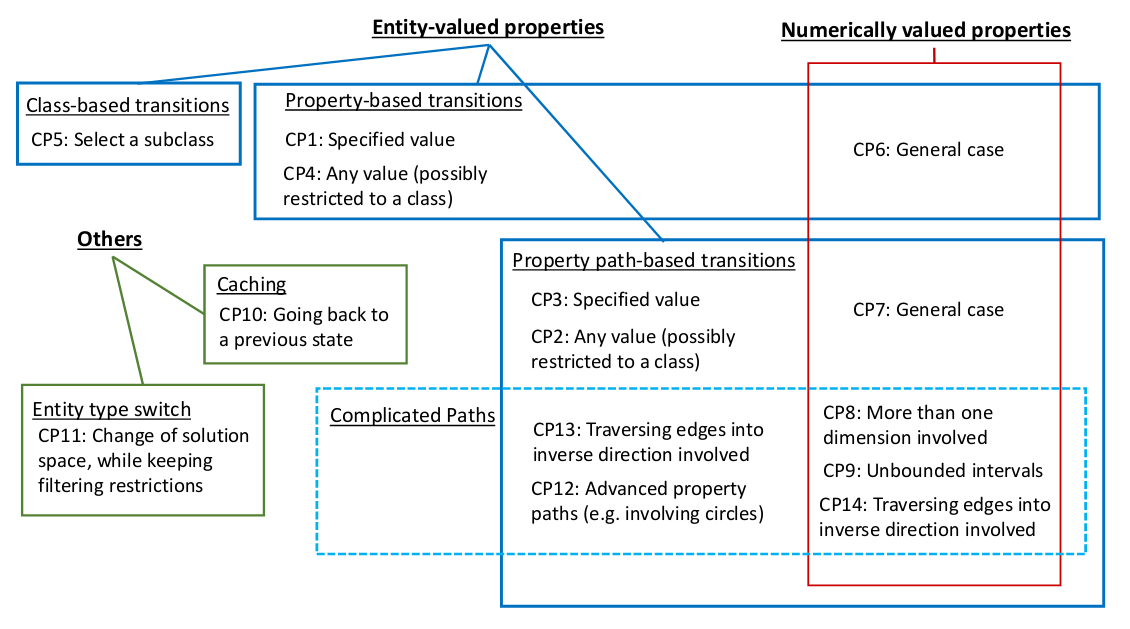
\includegraphics[width=\textwidth]{images/cps}
\caption{Overview of chokepoints}
\label{fig:chokepoints}
\end{figure}

%\todo{This list is extensible}
A chokepoint is essentially a named faceted browsing interaction followed by a subsequent information need (such as facet counts or available values), whose performance and correctness
is subject to evaluation. The obtained results define
the values of the key performance indicators of the benchmark.
An overview of the chokepoints supported by our system is depicted in~\autoref{fig:chokepoints}.
These chokepoints were proposed in~\cite{petzka}, in which they are implemented on some specific instances using parametrisation of hand-crafted SPARQL query templates. In our system, they are implemented in a generalised and universal fashion.


\begin{description}
\item[CP1] Property value based transition\\
Find all instances which, additional to satisfying all restrictions defined by the state within the browsing scenario, have a certain property value
\item[CP2] Property path based transition\\
Find all instances which additionally realise this property path with any property value
\item[CP3] Property path value based transition\\ 
Find all instances which additionally have a certain value at the end of a property path.
N.b. This is CP1 with a property path instead of a property
\item[CP4] Property class value based transition\\
Find all instances which additionally have a property value lying in a certain class
\item[CP5] Transition of a selected property value class to one of its subclasses \\
For a selected class that a property value should belong to, select a subclass
\item[CP6] Change of bounds of directly related numerical data\\
Find all instances that additionally have numerical data lying within a certain interval behind a directly related property
\item[CP7] Change of numerical data related via a property path of length strictly greater than one edge\\
Similar to 7, but now the numerical data is indirectly related to the instances via a property path
\item[CP8] Restrictions of numerical data where multiple dimensions are involved\\
Chokepoints 7 and 8 under the assumption that bounds have been chosen for more than one dimension of numerical data, here, we count latitude and longitude numerical values together as one dimension
\item[CP9] Unbounded intervals involved in numerical data\\
Chokepoints 7,8,9 when intervals are unbounded and only an upper or lower bound is chosen
\item[CP10] Undoing former restrictions to previous state\\
Go back to instances of a previous step
\item[CP11] Entity-type switch changing the solution space\\
Change of the solution space while keeping the current filter selections
\item[CP12] Complicated property paths or circles\\
Chokepoints 3 and 4 with advanced property paths involved
\item[CP13] Inverse direction of an edge involved in property path based transition\\
Property path value and property value based transitions where the property path involves traversing edges in the inverse direction
\item[CP14] Numerical inequality restriction over a property path involving the inverse direction of an edge\\
Additional numerical data restrictions at the end of a property path where the property path involves traversing edges in the inverse direction
\end{description}


\subsection{Configuration and Output}
The benchmark is configured with an RDF document describing the number of faceted search scenarios to generate as well as how many interaction/chokepoints to apply within a scenario. The application of chockepoints is controlled using a non-deterministic-automaton (NFA). This makes it possible to configure the benchmark generator to simulate natural behavior more closely. For example, this snippet in ~\autoref{fig:config-and-output} shows, that the first interaction is always the selection of a certain type. The min/max ranges are substituted with new concrete values on every scenario. The output is simply a set of RDF resources with the SPARQL query string and metadata attached.


\begin{figure}
\centering
\bgroup
\def\arraystretch{1.5}
\begin{tabular}{m{8cm}m{8cm}}
\begin{lstlisting}[language=sparql, linewidth=7cm]
:defaultScenarioConfig
  a o:ScenarioConfig ;
  o:randomSeed 1000 ;
  o:scenarioLength [ o:min 4; o:max 8;
    o:type xsd:integer] ;
  o:numScenarios 10 ;
  o:numWarmups 2 ;
  o:nfa [
    o:startState o:state1 ;
    o:transition [
      o:from o:state1 ;
      o:to o:state2 ;
      o:key "cp5" ;
      o:weight [ o:min 0.6 ; o:max 1.0 ]
    ] ;
    # More states
  ] .
\end{lstlisting}

&

\begin{lstlisting}[language=sparql, linewidth=7cm]
:scenario1-0
  o:chokepointId 5 ;
  o:queryId 0 ;
  o:scenarioId 1 ;
  o:sequenceId 0 ;
  o:task "SELECT * { ... }"
  o:expectedResult "..." ;
  o:expectedResultSize 1001 .
\end{lstlisting}

\\

\end{tabular}
\egroup
\caption{Benchmark generator configuration and output models}
\label{fig:config-and-output}
\end{figure}


\section{Evaluation}
\label{sec:evaluation}
For evaluation, we created an integration of our benchmark generator with the HOBBIT Platform\footnote{\url{http://project-hobbit.eu/}}.
HOBBIT is a benchmarking platform that follows the FAIR principles (Findability, Accessibility, Interoperability, and Reusability)\footnote{\url{https://www.nature.com/articles/sdata201618.}}.
It hosts 5 triple stores which participated in the faceted browsing challenge, namely
Apache Jena Fuseki 3.6.0, VOS for all, GraphDB Free 8.5, Virtuoso v8.0 and Blazegraph.

For benchmark data, we generated datasets using the \emph{Public Transport RDF Dataset Generator} PoDiGG~\cite{podigg}. The generated data has a small schema with main entities being stops, routes (sequences of stops) and connections (instances of routes at certain times). Using our framework, we generated a faceted browsing benchmark using a Virtuoso 7.2.5\footnote{\url{https://virtuoso.openlinksw.com/}} as the reference triple store (via the tenforce/virtuoso docker image\footnote{\url{https://github.com/tenforce/docker-virtuoso}}). The Virtuoso instance used as the reference triple store differed from the one that acted as the system under test (SUT).

The systems under tests' query execution time was limited to 5 minutes. Although we experimented with data set sizes up to 10M triples, it turned out, that even on a small data set with 500K triples, two systems were still not able to complete all queries in less than 5 minutes. \autoref{fig:eval-performance} shows the results for a setup with 234 unique queries across 322 tasks (CP10 is the undo operation, hence some duplicate queries are intentional), 24 queries were used as warm-up (which amounts to approx 20\%). All systems yielded the same result sets on all tasks, and thus performed correctly. \autoref{fig:eval-performance-cp} shows the results per chokepoint, which indicates that all of them were applied in the generated benchmark.
We also conducted experiments with DBpedia data, however, its schema graph has too many possible combination of paths. As such, we defer to future work before we can select a sensible subset of DBpedia to evaluate the path finding components on.
An interesting aspect with a DBpedia dataset with 170 million triples was, that a simple aggregation for facet values of~\autoref{lst:simple-facet} took with approximately 3min30sec the same time using a Virtuoso VOS 7.2.4 (single core) deployed on a developers' DELL XPS13 9360 notebook and a Supermicro server with 8GB and 64GB allocated to it. Hence, the aggregation is -- for this triple store -- a CPU bound operation.

\begin{figure}
\centering
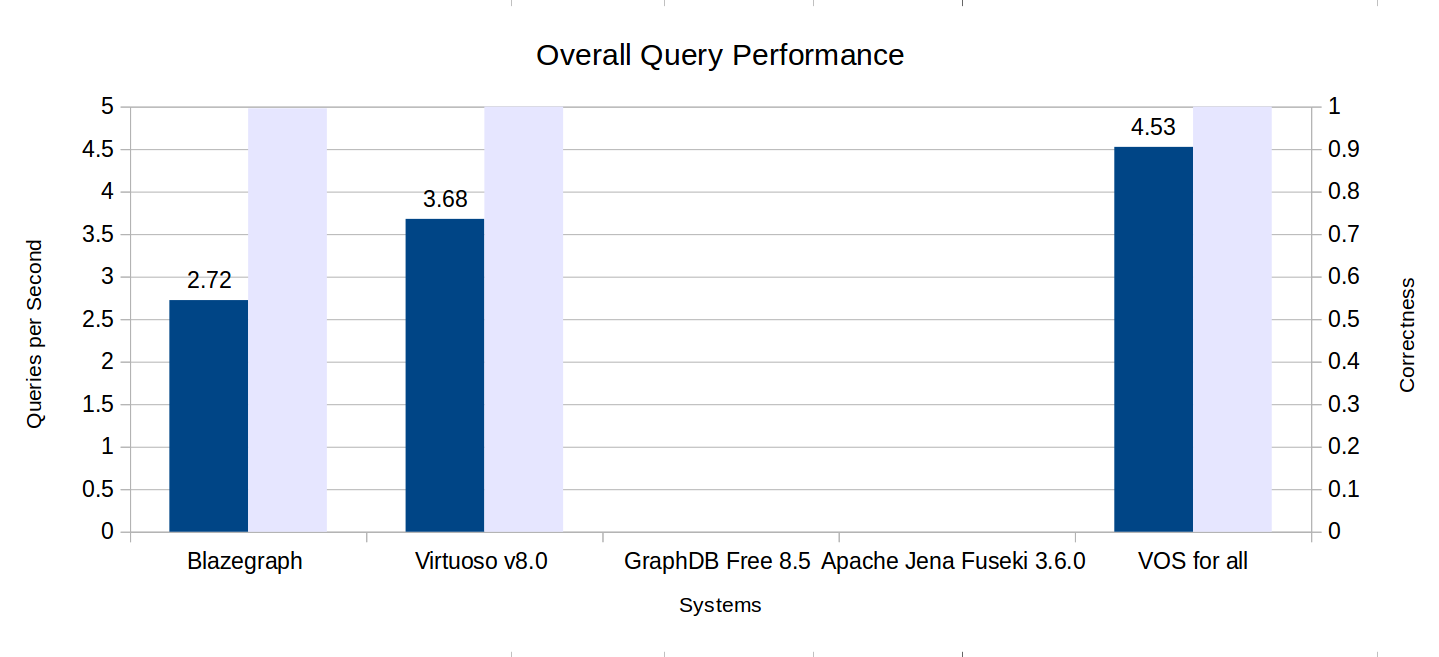
\includegraphics[width=\textwidth]{images/eval-performance-chart.png}
\caption{HOBBIT Benchmark Results on PoDiGG}
\label{fig:eval-performance}
\end{figure}

\begin{figure}
\centering
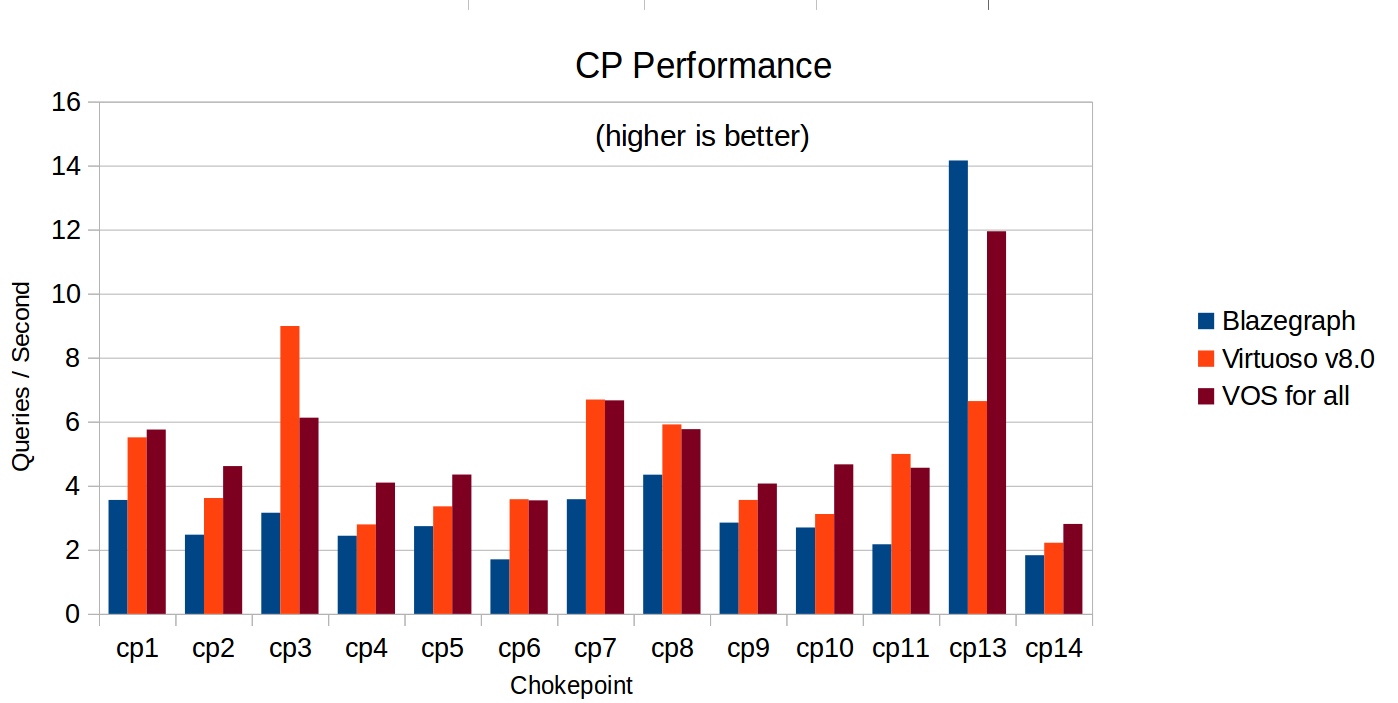
\includegraphics[width=\textwidth]{images/eval-performance-chart-cp.png}
\caption{Performance of queries by chokepoint}
\label{fig:eval-performance-cp}
\end{figure}


\section{Related Work}
\label{sec:related-work}
The first faceted search approaches were developed in the 1990s for information retrieval systems. They combined the paradigms of \textit{structured retrieval} and \textit{similarity-based ranking} by leveraging the benefits of constraint-based querying over large data sources. Since then, the approach has proven to be tremendously useful for search applications. Hence, faceted browsing is ubiquitous on the Web today. Most if not all major online applications provide at least some degree of faceted browsing feature to navigate the metadata records of their items \cite{tunkelang}.\\ 
This is why this approach has not only been applied for unstructured text documents, but also for knowledge graph data. To this date, a couple of prototypes facilitate indexing and faceted browsing of RDF data \cite{cheng, davies, hahn, waitelonis, moreno-vega}. But since these systems require an index at runtime, they offer limited flexibility regarding the kinds of queries that can be posed. Hence, entity types or facet combinations are hard-wired into the system and can not be easily adapted to changing user needs or different kinds of schemas and data models \cite{wenige}. Other approaches overcome these problems by facilitating ad-hoc exploration and facettation of RDF data from triple stores \cite{stadler, kremen, ferre, arenas}. The query-based faceted search paradigm goes back to Ferr\'{e} et al. who introduced a high level query language to integrate SPARQL querying and property-based navigation \cite{ferre}. The \textit{facete} and the \textit{SemFacet} engines \cite{arenas} have a similar approach. They offer faceted browsing capabilities for triple stores or databases that expose a SPARQL endpoint \cite{stadler}.\\
Besides enabling end user navigation, ad-hoc RDF-based faceted search also facilitates statistical inspection. In this line of research faceted exploration is also related to Online Analytical Processing (OLAP) systems since both approaches process multi-dimensional data \cite{ben-yitzhak}. But while OLAP cubes follow a predefined metadata schema, query-based facet engines are more flexible in regard to the dimensions that can be explored.\\
However, SPARQL-based ad-hoc processing comes at the cost of performance as both path traversal and aggregation operations have to be executed at runtime. Thus, there is a need for testing triple stores with regard to their fitness for out-of-the-box browsing on various data sources and schemas. 
Only then can application providers be supported in identifying suitable infrastructures (e.g. triple stores or hardware resources) as well as potential performance bottlenecks. There exists a wide variety of RDF-based facet engines. However, evaluation methods and datasets for these systems are not yet standardized \cite{tzitzikas}. Hence, there is a need for domain-independent tools to generate faceted browsing benchmarks for different use cases in order to reproduce performance tests throughout different evaluation runs \cite{moreno-vega}. Currently, a considerable amount of benchmarks is available to evaluate the general performance of triple stores (e.g., LUBM \cite{guo}, SP2 \cite{schmidt}, BSBM \cite{bizer}, WatDiv \cite{aluc} and Geographica \cite{garbis}). On the other hand, only a few attempts have been reported in the literature that evaluate RDF-based faceted browsing. For instance, Arenas et al. describe a generic approach with which their \textit{SemFacet} engine can be tested \cite{arenas}. Petzka et al. present a benchmark dataset for different faceted queries \cite{petzka}. What is currently missing, however, is a faceted browsing benchmark generator that can be configured for various schemas, data sources and hence application domains. But in order to set up a generator tool, we need an understanding of the upper bounds of ad-hoc faceted querying. Hence, it has to be investigated which query types are actually feasible for a SPARQL-based facet navigator and can still be answered within reasonable response time limits. Thus, a  meta-benchmarking is also required. To the best of our knowledge, we are the first to present a toolset on schema-agnostic (meta-)benchmarking for faceted browsing over SPARQL endpoints. 

%\section{Discussion}
%Maybe it makes sense to add such a section.
%Limitations of the benchmark - only disjunctive queries tested
%Limitations of the platform (no sparql proxy - always need to deploy -> heavy weight process, no support for caching of generated artifacts, determinism)

%\subsection{Faceted Browsing Benchmark}
%DBpedia, LGD, und Freebase


\section{Conclusions and Future Work}
\label{sec:conclusions}
In this work we presented a schema-agnostic faceted search benchmark generation framework for triple stores.
Performance of SPARQL-based faceted search depends mainly on the triple stores' capabilities of aggregating and counting data. Some benchmarked systems reached timeouts on query loads on relatively small dataset sizes. This suggests, that even today, live faceted search on SPARQL endpoints is associated with a high performance cost. As our evaluation of a simple aggregation on a large volume of data shows, interactive performance on such data is only achievable by means of indexing.
Indexing can be performed on different levels: While it is possible to cache entirely on the SPARQL level, it may be advantageous to index on the level of a language for SPARQL-based faceted search. The reason is, that simple domain specific operations, such as "yield all facet values", may result in relatively complex SPARQL queries (as shown in~\autoref{fig:engine-real-example}).
Our resource thus provides fundamental functionality for these kinds of future research:
On the one hand, creation of such an index (via SPARQL) requires assembling exactly the queries our faceted search engine generates. On the other hand, our DSL provides a high level abstraction for faceted search queries which may be suitable for use in conjunction with advanced indexing strategies.
In any case, our benchmark generator can be used to automatically evaluate faceted search over arbitrary RDF datasets in order to detect potential performance issues.

%\section*{Acknowledgements}
%This work was supported by grants from the EU H2020 Programme for the projects HOBBIT (GA no. 688227) and QROWD (GA no. 732194).

\begin{thebibliography}{99}
\bibitem{podigg} Taelman, R.; Verborgh, R.; Nies, T. D. \& Mannens, E. (2017), PoDiGG: A Public Transport RDF Dataset Generator., in Rick Barrett; Rick Cummings; Eugene Agichtein \& Evgeniy Gabrilovich, ed., 'WWW (Companion Volume)', ACM, pp. 843-844.
\bibitem{aluc} Alu\c{c} G, Hartig O, \"{O}zsu MT, Daudjee K (2014). Diversified stress testing of RDF data management systems. In: International Semantic Web Conference, pp. 197-212. 
\bibitem{arenas} Arenas M, Grau BC, Kharlamov E, Marciuška Š,  Zheleznyakov D (2016). Faceted search over RDF-based knowledge graphs. Journal of Web Semantics, 37, pp. 55-74.
\bibitem{ben-yitzhak} Ben-Yitzhak O, Golbandi N, Har'El N, Lempel R, Neumann A, Ofek-Koifman S, Yogev S. (2008). Beyond basic faceted search. In: Proceedings of the 2008 International Conference on Web Search and Data Mining, pp. 33-44. 
\bibitem{bizer} Bizer C, Schultz A (2009). The Berlin SPARQL benchmark. International Journal on Semantic Web and Information Systems (IJSWIS), 5(2), pp. 1-24.
\bibitem{cheng} Cheng G, Ge W, Qu Y (2008). Falcons: searching and browsing entities on the semantic web. In Proceedings of the 17th international conference on World Wide Web, pp. 1101-1102.
\bibitem{davies} Davies J, Weeks R (2004). QuizRDF: Search technology for the semantic web. In: Proceedings of the 37th Annual Hawaii International Conference on System Sciences.
\bibitem{ferre} Ferr\'{e} S, Hermann A (2012). Reconciling faceted search and query languages for the Semantic Web. Int. J. Metadata, Semantics and Ontologies, 7(1), pp. 37-54.
\bibitem{garbis} Garbis G, Kyzirakos K, Koubarakis M (2013). Geographica: A benchmark for geospatial RDF stores. In: International Semantic Web Conference, pp. 343-359. 
\bibitem{guo} Guo Y, Pan Z, Heflin J (2005). LUBM: A benchmark for OWL knowledge base systems. Web Semantics: Science, Services and Agents on the World Wide Web, 3(2-3), pp. 158-182.
\bibitem{hahn} Hahn R, Bizer C, Sahnwaldt C, Herta C, Robinson S, Buergle M, Scheel U (2010). Faceted wikipedia search. In: International Conference on Business Information Systems, pp. 1-11. Springer, Berlin, Heidelberg.
\bibitem{kremen} Kremen P, Saeeda L, Blaško M. (2018). Dataset dashboard–a SPARQL endpoint explorer. In: CEUR Workshop Proceedings of Fourth International Workshop on Visualization and Interaction for Ontologies and Linked Data, VOILA.
\bibitem{moreno-vega} Moreno-Vega J, Hogan A (2018). GraFa: Scalable Faceted Browsing for RDF Graphs. In: International Semantic Web Conference, pp. 301-317. Springer, Cham.
\bibitem{petzka} Petzka H, Stadler C, Katsimpras G, Haarmann B, Lehmann J (2017). Benchmarking faceted browsing capabilities of triplestores. In: Proceedings of the 13th International Conference on Semantic Systems, pp. 128-135.
\bibitem{schmidt} Schmidt M, Hornung T, Lausen G, Pinkel C (2009). SP2Bench: a SPARQL performance benchmark. In: 2009 IEEE 25th International Conference on Data Engineering pp. 222-233. 
\bibitem{stadler} Stadler C, Martin M, Auer S (2014). Exploring the web of spatial data with facete. In: Proceedings of the 23rd International Conference on World Wide Web, pp. 175-178.
\bibitem{tunkelang} Tunkelang D (2009). Faceted search. Synthesis lectures on information concepts, retrieval, and services, 1(1), pp. 1-80.
\bibitem{tzitzikas} Tzitzikas Y, Manolis N, Papadakos P (2017). Faceted exploration of RDF/S datasets: a survey. Journal of Intelligent Information Systems, 48(2), pp. 329-364.
\bibitem{waitelonis} Waitelonis J, Sack H (2012). Towards exploratory video search using linked data. In: Multimedia Tools and Applications, 59(2), pp. 645-672.
\bibitem{wenige} Wenige L, Ruhland J. Similarity-based Knowledge Graph Queries for Recommendation Retrieval. 
\end{thebibliography}




\section{Introduction}
\label{sec:introduction}

The growth of the Linked Open Data (LOD)
cloud\footnote{\url{http://lod-cloud.net/}}
goes hand in hand with an increasing amount of geospatial information being made available
for online querying via SPARQL.
For instance, the community projects DBpedia and LinkedGeoData provide access
to more than 1.3 million and 2 billion point geometries based on Wikipedia and
OpenStreetMap data, respectively. Government agencies have started maintaining
public SPARQL endpoints, such as \emph{Ordnance
Survey}\footnote{\url{http://data.ordnancesurvey.co.uk}}
and the \emph{European Environment
Agency}\footnote{\url{http://semantic.eea.europa.eu/sparql}}.
The latter, for instance, hosts
% 9.321 RDF graphs, of which
123 RDF graphs that contain a sizable number of resources described using
the WGS84 vocabulary\footnote{\url{http://www.w3.org/2003/01/geo/wgs84_pos}}.
%instances.

%\footnote{\url{http://data.ordnancesurvey.co.uk/datasets/os-linked-data/explorer/sparql}}
% \footnote{\url{http://semantic.eea.europa.eu/sparql}}.
%The importance of geospatial data has also been recognized by many RDF store
%implementors, who over the past few years added and enhanced spatial support in
%their products.
Yet, the user friendly exploration of spatial data accessible via public SPARQL remains a
major challenge, especially due to performance, volume, scalability and UI
complexity issues.
In this demo, we present the spatial data exploration and
visualization application \emph{Facete}, depicted in
\autoref{fig:facete-screenshot}.
%\todo{Mention that Jassa makes these re-usable}
Facete is a client-side JavaScript application, which interacts with a server-side SPARQL endpoint.
The major problem when exploring spatial data is that the spatial dimension is in most cases not directly attached to all the data items.
For example, a dataset about multi-partner research projects would contain entities for the projects itself, the project partners, their legal entities, the branch offices of these legal entities and finally the cities they are located in.
If we want to visualize such data intuitively, we need to determine the path from data items of interest to the indirectly related spatial entities.
Facete solves this problem with a automatic discovery of the most likely property path.
Compared to other faceted browsers, Facete not only allows to constrain over facets of a particular set of entities, but over facets across full property paths.
This allows to explore data more intuitively and in ways previously impossible.

In the remainder, we explain Facete's user
interface in \autoref{sec:facete},
followed by a description of a use case
scenario in \autoref{sec:use-case}.
In \autoref{sec:concepts} we briefly outline the conceptual background of Facete's main components. Subsequently,
\autoref{sec:related-work} discusses related work. Finally,
\autoref{sec:conclusions} concludes and gives pointers to
future work.
Comprehensive accompanying material including the open-source code, screencasts and documentation can be found at \url{http://facete.aksw.org}.
%It is noteworthy, that Facete as described in this submission is an application.
%Application code itself is not aimed at reusability, in contrast to library code.
Under the umbrella of the
\emph{JAvascript Suite for Sparql Access
(Jassa)}\footnote{\url{https://github.com/GeoKnow/Jassa}} project, we are
working on making Facete's core components available as reusable library components,
which developers may reuse and customize as needed.


%The European Environment Agency maintains a SPARQL
%endpoint\footnote{\url{http://semantic.eea.europa.eu/sparql}} has started
%% publishing RDF, of which \todo{number} use the wgs84 vocabulary.
%9.321 named graphs having at least a single instance described using the WGS84
%geo positioning
%vocabulary\footnote{\url{http://www.w3.org/2003/01/geo/wgs84_pos}}.
%Among those graphs there are 123 graphs having more than 50 of such
%instances.


%%\todo{Mention deployment}
%%TODOyay\footnote{\url{http://open-data.europa.eu/semmap/}}

\section{The Facete SPARQL Explorer}
\label{sec:facete}
Facete is a Single Page Application (SPA) whose user interface comprises several
UI components, which are depicted in~\autoref{fig:facete-screenshot} and
explained in the following.
In the top area, there are elements that enable the user
to select a SPARQL endpoint and chose from one or more of its contained named graphs.
The main panel is divided into three columns containing a set of widgets with
the following functionality:
%\todo{Motivate that faceted search is superior (to what?) because one cannot
%hit dead ends} \todo{In conclusion, mention how the faceted search can also be
%% applied to statistical data, i.e. it is possible to create a datacube closure
%over ANY set of RDF resources; the facet module already does filtering by an
%arbitrary number of correlated dimensions.}
\emph{1. Selection.}
The first widget, labeled \emph{Facet}, shows a
  facet tree that corresponds to the properties of all resources that match the
  set constraint.
  If there are no constraints, all resources that appear as a subject in the
  selected graphs are matched.
  Three actions can be performed for node in the facet tree:
  A click on the facet's name lists the facet's values in the
  \emph{Facet Value} widget, where these values can be used for defining
  constraints. Clicking the caret symbol toggles the display of
  corresponding child facets. These are the properties of the the selected facet's values.
  Lastly, a facet can be pinned as a column to the \emph{Table View}.
  Note, that the root of the facet tree is formed by a facet labelled
  \emph{Item}. This facet's values correspond to the set of resources in
  subject positions of the selected RDF graphs.
The \emph{Facet Values} widget enables a user to paginate
  through a selected facet's values and optionally filter these values by a
  search term. Furthermore, clicking the checkbox next to a value creates a
  constraint.
The \emph{Filters} widget lists all active constraints.
  Individual constraints can be removed by clicking their entry, whereas the  
  \emph{Clear Filters} button purges them all. 


\emph{2. Data.}
The middle area contains the \emph{Table View}, which
  lists a table whose content is based on resources that match the active constraints
  and the facets that were pinned as columns.
  Columns can be sorted by clicking the caret icons. Multiple orders are
  supported by holding the shift key down while clicking.

\emph{3. Geographical.}
The \emph{Geo-Link} drop down menu enables the user to choose from
  property paths connecting the resources that match the constraints with those
  that can be shown on the map. By default, the option \emph{automatic} is
  enabled, which always picks the shortest path among the found ones.
The \emph{Map} widget displays markers corresponding to the
  selected resources and the geo-link. Blue boxes indicate areas that contain
  too many markers to be shown at once. These boxes disappear when
  sufficiently zoomed in. Clicking a marker shows its details in the
  \emph{Detail View}.
The \emph{Detail View} shows the excerpt of the \emph{Table View} that
  corresponds to the selected marker(s).

\begin{figure*}[t]
\centering
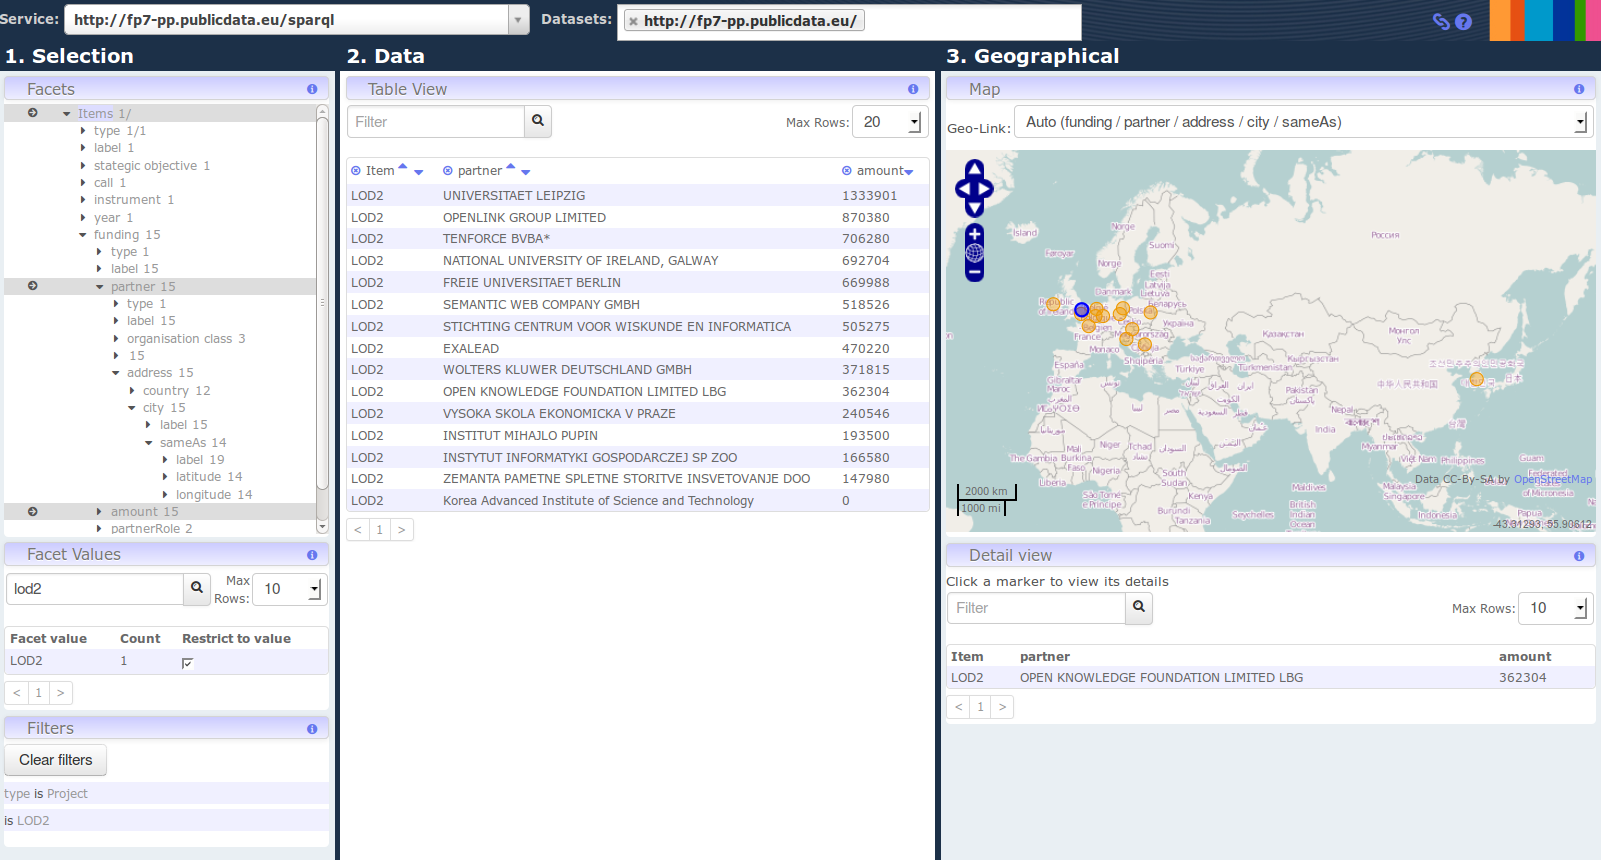
\includegraphics[width=\textwidth]{images/2013-12-19-odp-facete-2.png}
\caption{Screenshot of Facete showing information from the CORDIS dataset about FP7 research funding.}
\label{fig:facete-screenshot}
\end{figure*}


\section{A sophisticated Use Case}
\label{sec:use-case}
We demonstrate Facete in a use case scenario, which
to the best of our knowledge, none of the existing SPARQL browsers can serve
easily.

The dataset about \emph{ICT research projects under EU-FP7} 
\footnote{\url{http://open-data.europa.eu/en/data/dataset/ict-research-projects-under-eu-fp7}},
for which an RDF version
exists\footnote{\url{http://fp7-pp.publicdata.eu}}, 
contains comprehensive information about funded projects, partner organizations and particularly also how much money was granted to partners in FP7-ICT
projects.
The most important classes and their relations are as follows:
Every \emph{Project} is related to a set of \emph{Fundings} (grants), whereas each
instance represents the amount of money granted to a single project
partner (beneficiary). %Partners who received  (\todo{beneficiary}).
%Each funding targets a beneficiary, whereas beneficiaries may receive multiple
%fundings.
Partners carry address information, which includes resources for
the country and city. The cities' geo-coordinates were
obtained based on interlinking them with
\emph{LinkedGeoData}\footnote{\url{http://linkedgeodata.org}}.
This model is depicted in~\autoref{fig:relation-example}.
\begin{figure}
\centering
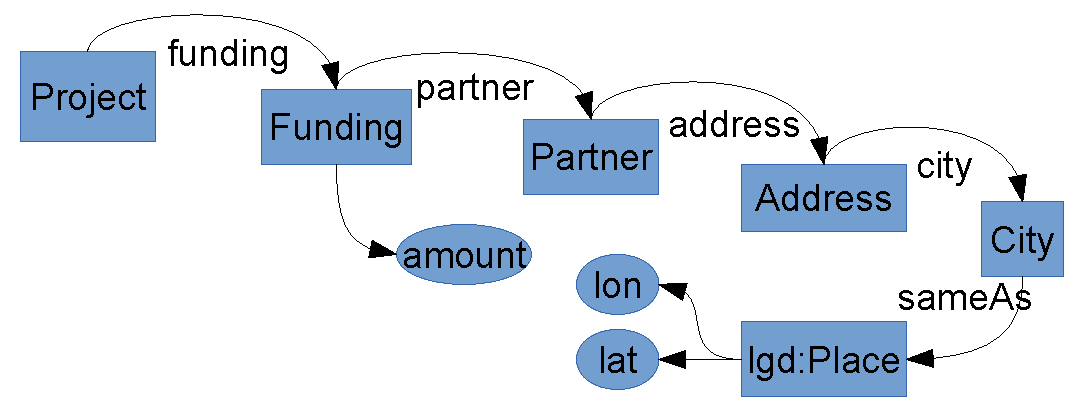
\includegraphics[width=0.5\textwidth]{images/RelationExample}
\caption{Excerpt of the CORDIS dataset model showing the path how projects are related to geo-coordinates.}
\label{fig:relation-example}
\end{figure}

There are several questions one may ask, such as:
What are the projects related to a certain country? 
Where are the partners of a particular project located?
How much money was granted to partners in a specific project?

With Facete, the following procedure can be performed to answer these questions:
\begin{itemize}
  \item First, select the \emph{type} facet, and constrain it to the value
  \emph{Project}. The main table will now only list project names, and the map
  component will automatically determine connections that link projects
  to coordinates.
  \item A project is related to a country if there is at least one project
  partner located in that country.
  Expanding the \emph{funding} facet will list several nested facets, including
  \emph{partner} and \emph{amount}.
  We can then dive deeper into the facet tree by expanding first \emph{partner}
  and then \emph{address}. This reveals a \emph{country} facet. Clicking it's
  label lists its corresponding facet values, which can then be
  constrained to a country of interest, such as ``Germany''.
  The main table, as well as the map, will update to only show projects related
  to this country.
  \item A project can then be singled out by clicking the
  label of the \emph{Item} facet and constraining it to the resource of
  a specific project, such as \emph{LOD2}. The map view now only shows
  those partners that are located in the previously selected country. 
  \item So far, the main table only listed names of projects.
  Pinning the \emph{partner} and \emph{amount} facets to the main table shows
  this project's related information. Drop the constraint on countries for the
  map to show partners world wide.
\end{itemize}

Note that this use case stands exemplary for a large number of similar use cases involving spatial data.
%, such as depicting courts on a map that were responsible for a given set of rulings.


%A current limitation of the implementation is, that aggregations are not yet
%supported on the user interface level. Hence, analytical
%queries, such as 
%``What is the total amount of funding a partner received?'
%are left for future work.
 


%Even though the dataset is hosted as Linked Data, it would require substantial
%efforts collecting the information just via link traversal.
%\todo{What i mean is: Even though Linked Data is machine readable, it lacks the
%query capabilities to satsify the use case.}

%\todo{even if we are only interested in how much money a partner received in a
%project}
%Clearly, above questions can be answered with SPARQL, but in a first step
%this raises additional questions:
%Which properties (such as types) exist in the dataset so that they can be
%used for filtering? How are resources related to the geometric information that
%is needed to visualize the data on a map?

%We devise Facete 

%TODO Mention than faceted concepts map nicely to RDF


\section{Concepts}
\label{sec:concepts}

In this section we briefly outline the key concepts used in Facete, which are
related to faceted search, detection of property paths that connect
concepts and dealing with large amounts of spatial data.

\subsection{Facted Search}
There are several systems that support faceted filtering of a set of RDF resources by
either immediate (possibly predefined) properties. However, faceted search over
indirectly related properties is much more challenging. Facete's approach is
based on the following key concepts:
\begin{itemize}
\item A \emph{SPARQL concept} is a pair
comprising a SPARQL graph pattern and a variable thereof.
As such, it intentionally describes a set of resources.
For instance, the pair \emph{(\{?s a Project\}, ?s)} describes the set of
project resources. SPARQL concepts are the key enabler for indirect faceted search.
Internally, Facete uses them to represent \emph{any} set of resources, i.e.
the set of facets, the set of child facets, the set of facet values and the set
of resources with geometric information.
\item \emph{Property Steps} are used to navigate from a set of resources to a
related set of resources by following a specific property.
A direction attribute determines whether to follow that property in forward or
inverse direction.
Hence, a destination SPARQL concept can be obtained from a given origin SPARQL
concept and a property step.
\item A \emph{Property Path} is a sequence of property steps. 
\item \emph{Constraint Specifications} express constraints via references to
property paths. Constraint specifications are internally translated to
corresponding SPARQL graph patterns.
\end{itemize}

\subsection{Finding Connections between SPARQL Concepts}
Due to data modeling, the spatial dimension is in most cases not directly attached to instances of a certain type.
%Also, properties with different names may be used to connect a resource to
%corresponding geometric information.
%For example, research projects have partner organizations, which have offices,
%which are again linked to cities and these finaly have geo-coordinates being
% representable on a map.
In order to visualize the spatial dimension of such objects efficiently and intuitively we need an approach to find connecting property paths between two arbitrary SPARQL concepts efficiently.
As our use case demonstrates, these paths can become relatively
long, and naive path discovery approaches are not feasible.
Our approach is outlined as follows:
Because we are only interested in the detection of property paths, we
pre-compute a \emph{property join summary}. The basic SPARQL query for this
purpose is:
\begin{lstlisting}
CONSTRUCT { ?p1 :joinsWith ?p2 } {
  { SELECT DISTINCT ?p1 ?p2 {   
      ?a ?p1 [ ?p2 ?b ]
} }
\end{lstlisting}

Conceptually, we could search for arbitrary complex paths, such as ones that
include cyclic (same property followed multiple times in the same direction)
and zig-zag (forward and backward on the same
property
traversals. However, for our use cases the restriction to directed
acyclic paths leading from a \emph{source concept} to a \emph{target concept}
was sufficient: We query the source concept for all of its properties $?p$, and
conceptually add triples \emph{(:source :joinsWith $?p$)} to the join summary.
Thereby \emph{:source} is a distinguished resource representing the source
concept. From a target concept's graph pattern, such as \emph{(?s geo:long ?x ;
geo:lat ?y, ?s)}, we can infer that we need to search for properties that
according to the join summary are connected to both geo:long and geo:lat.
As a consequence, we can query the join summary for a set of candidate target
properties using:
\begin{lstlisting}
SELECT DISTINCT ?p { ?p :joinsWith geo:long ; joinsWith geo:lat }
\end{lstlisting} 
If the extensions of the source and target concepts have resources in
common, this query's result set includes \emph{:source} as a candidate.

We can now search for candidate paths on the join summary that connect
\emph{:source} with each of the candidate properties. For each candidate path we
then fire an ASK query to check whether the given dataset contains an instance of it.
Those paths that actually exist, are then listed in Facete's Geo-Link drop down
box.

Note, that this approach is independent of any concrete vocabulary.

\subsection{Display of large Amounts of Geometries}
Some spatial RDF datasets, such as DBpedia or Freebase, contain
significantly more spatial information than what can performance and bandwidth wise be
reasonably retrieved and displayed on a map in a web application.
Facete handles such cases using a quad tree data structure:
\begin{itemize}
  \item Based on the users constraints on the facets and the geo-link,
  a corresponding SPARQL concept, named \emph{geo-concept}, is created. The
  geo-concept specifies the set of resources to be shown on the map.
  \item A count of the number of instances matching the geo-concept is
  requested. If the count is below a configured threshold, all instances are
  retrieved at once and placed into the root node of the quad tree.
  \item If this count exceeds the threshold, the extent of the whole map is
  split recursively into four tiles of equal size. The recursion
  stops if either a maximum depth is reached, or if the tiles have reached a
  certain relative size when compared to the map viewport (e.g. when about
  4x4 tiles are visible).
  For each tile, the
  geo-concept is then modified to only refer to resources within that tiles'
  bounding box. A tile's resources are only retrieved, if the new count is again below a
  configured threshold.
  \item Tiles that still contain too many geometries are rendered as boxes on
  the map.
\end{itemize}
An example of such display is shown in~\autoref{fig:markers-freebase}, which
shows a subset of the approx. 20.000 resources with geo-positions in Germany.
For each set of constraints, Facete creates a new quad tree that acts as a cache
for the user's current configuration.
%Also, Facete includes a client side SPARQL result set
%pagination component which effectively levers out SPARQL endpoint's result set
%limits.

%Facete includes a client side pagination component that alleviates
%possible limitations set by SPARQL endpoints result set 
\begin{figure}
\centering
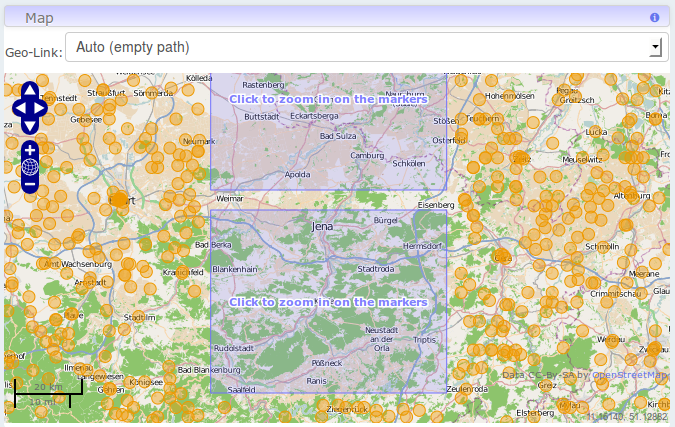
\includegraphics[width=0.5\textwidth]{images/facete-mii}
\caption{Display of Freebase instances in Germany.}
\label{fig:markers-freebase}
\end{figure}



\section{Related Work}
\label{sec:related-work}
The \emph{RelFinder} system~\cite{2009_relfinder} is capable of finding
property paths connecting a pair of \emph{resources}, whereas
Facete searches for paths between SPARQL \emph{concepts}.
Over the past decade, faceted search has become omnipresent, such as in
web shop and content management systems.
\emph{Apache Solr}\footnote{\url{http://lucene.apache.org/solr/}} is a popular system
that offers extensive faceted search features, however, it does not offer native
SPARQL support and thus requires pre-processing of RDF data.
\emph{Rhizomer}~\cite{2013_rhizomik} and the
\emph{Virtuoso faceted
browser}\footnote{\url{http://virtuoso.openlinksw.com/dataspace/dav/wiki/Main/VirtuosoFacetsWebService}}
support changing the focus from one set of resources to a related one
(known as pivoting). However, with these systems, the user actually navigates
between related list views of resources, whereas in Facete the user pins facets
as new columns to the table view.
%\emph{Sparallax}
%\footnote{\url{http://sparallax.deri.ie}}


%Pivoting (refocusing) 
% unconstrained and relational 

%Exhibit is often used for RDF data, it uses
%Facete offers this functionality directly on RDF.  


%While \todo{deri paper} investigate federated search based on SPARQL 1.1
%federation, we envision that SPARQL query federation engines, such as 
%FedEx and TopFed offer 

%Flint, Sparql-ed, YASGUI
%Ontowiki, (what about Calimachus?)


%Challenges:
%- Several geo vocabs - how to support them?
%- Large amount of spatial data

%- 
%Facete ful 
%\footnote{\url{http://geovocab.org}}
%\footnote{\url{}} georss
%\footnote{\url{http://www.opengeospatial.org/standards/geosparql}} geosparql
%\footnote{\url{http://docs.openlinksw.com/virtuoso/rdfsparqlgeospat.html}}


%\section{Implementation}
%github
%debian package
%Some limitations
%Computation of properties and their counts is affected by two dimensions:
%The current implementation of Facete attempts to retrieve all properties and
%their counts in a single query.
%Dimenions: Number of triples to scan - and number of distinct properties.
%This strategy works well for small datasets
%small datasets, sufficient constraints, few properties
%We are in the process af alleviating this limitation by 
%either small from the start, or thesufficiently constrained
%is based on the assumption that there is only a
%limited number of properties.
%DBpedia has \todo{count} properties, Freebase even.
%In the latter case, when excluding isbn numbers and users, still 100k remain.
%Initial experiments with DBpedia and Freebase
%showed that this assumpti


\section{Conclusions and Outlook}
\label{sec:conclusions}
In this demo we present \emph{Facete}, an advanced faceted browser
for SPARQL accessible data with geo-spatial capabilities.
We demonstrate Facete's potential based on a sophisticated use case
which requires retrieval of information from a set of
indirectly related resources. Users are empowered to create customizable a tabular data views showing attributes they are interested in. 
Based on related geometric information, these data are also shown on a map.
% and can browse these data on
%the map.
Facete's three key concepts are:
(1) The generic faceted filtering engine,
that supports showing and filtering by nested facets, (2) the property path
detection, which efficiently detects how resources can be shown on the map based
on indirectly related spatial information, and (3) how the system offers an
interactive map display even in the face of large amounts of geometric
information.

There are a number of directions for future work: One is adding support for aggregation
functions. Another logical step is to define more advanced views than
the current table and map.
Users should then be empowered to connect such views to their created data
table. For instance, once a user has defined a table which lists for each city
or country the total amount of money given to partners
located in it, then based on this information a heat map view could be rendered.
Our vision is, for the creation of visualizations from Linked
Data to become as simple as in spreadsheet applications,
where advanced chart and map visualizations can be created with a few clicks.
%Unlike conventional spreadsheets, however, the use of
%(quasi-)standard vocabularies could serve a convention over configuration
% approach

%Furthe definition of multiple data tables that may be related
%to each other. 



%A quad tree is a space partition tree where each node is partitioned into
% 4 children. Objects cannot 'sink' in a child node if they overlap a
% partition border. Loose quad trees allow child nodes to overlap to some
% extent, thus allowing objects overlapping the root nodes border
% potentially deeper in the tree.
 
%\section{Demonstration}


% We can add this for the camera-ready submission:
%\section{Acknowledgment}
%This work was supported by grants from the EU's 7th Framework Programme
%provided for the projects LOD2 (GA no. 257943) and GeoKnow (GA no. 611845).

%\bibliographystyle{abbrv}
%\bibliography{bibliography,../../bib/aksw}

%\end{document}




\section{Introduction}
\label{introduction}
The Semantic Web eases data integration tasks by providing an
infrastructure based on RDF and ontologies.
In order to employ the Web as a medium for data and information integration,
comprehensive datasets and vocabularies are required as they enable the
disambiguation and alignment of other data and information.
With \textit{DBpedia}~\cite{dbpedia_jws_09}, a large reference dataset
providing encyclopedic knowledge about a multitude of different domains is
already available. A number of other datasets tackling domains such as
entertainment, bio-medicine or bibliographic data are available in the emerging
Linked Data Web\footnote{See, for example, the listing at \url{http://ckan.net/group/lodcloud}
and an overview at \url{http://lod-cloud.net}.}.

With the \textit{OpenStreetMap} (OSM)\footnote{\url{http://openstreetmap.org}}
project, a rich source of spatial data is freely available.
It is currently used primarily for rendering various map visualizations, but has
the potential to evolve into a crystallization point for spatial Web data integration. 

The goal of our \textit{LinkedGeoData} (LGD) project is to lift OSM's data into
the Semantic Web infrastructure. We believe that this will 
simplify real-life information integration and aggregation tasks that require
comprehensive background knowledge related to spatial features.
Such tasks might
include, for example, to locally depict the offerings of the bakery shop next door, to map distributed
branches of a company, or to integrate information about historical sights along
a bicycle track.

The majority of our
data is obtained by converting data from the popular OpenStreetMap community project
to RDF and deriving a lightweight ontology from it. Furthermore, we perform interlinking
with \textit{DBpedia}, \textit{GeoNames} and other datasets as well as the
integration of icons and multilingual class labels from various sources.
As a side effect, we are striving for the establishment of an OWL vocabulary with the
purpose of simplifying exchange and reuse of geographic data.

After our initial LGD release in 2009~\cite{linkedgeodata}, we invested
substantial efforts in maintaining and improving LinkedGeoData, which include
improvements of the project infrastructure, the generated ontology, and data
quality in general. Our new contributions since then are:
\begin{itemize}
  \item A flexible system for mapping OpenStreetMap data to RDF:
  We now support nicer URIs (camel case), typed literals, language tags, and
  a simplified mapping of the OSM data to classes and properties.
  Together this accounts for an \emph{improved data quality}.
  \item \emph{Better support for ways:} Ways are OpenStreetMap entities
  used for modelling things such as streets but also
  areas (see Section~\ref{sec:OSM}).
  The geometry of a way (a line or a polygon) is now
  stored in a literal of the corresponding RDF resource, which makes it
  easy to e.g. display such a resource on a map. Furthermore, all nodes
  referenced by a way are available both via the Linked Data interface and the SPARQL endpoints.
  \item An \emph{improved REST interface} with integrated search functions.
  \item A new publicly accessible \emph{live SPARQL endpoint} that is being
  interactively updated with the minutely changesets that OpenStreetMap publishes.
  \item A simple \emph{republication method} of the corresponding RDF changesets so that LinkedGeoData
  data consumers can replicate our store.
  \item Direct \emph{interlinking} with \textit{GeoNames} and the \textit{UN FAO} data (interlinks with DBpedia have been updated).
  \item An \emph{improved LinkedGeoData browser}.
  \item Implementation of the \emph{Vicibit} application to facilitate the integration of LGD facet views in external web pages.
  \item Integration of appropriate \emph{icons and multi language labels} for LinkedGeoData ontology elements from external sources.
\end{itemize}

The paper is structured as follows: after introducing the OpenStreetMap project
in Section~\ref{sec:OSM}, we outline the LinkedGeoData architecture in
Section~\ref{sec:architecture}.
Subsequent sections explain, how the OSM data is transformed
into the RDF data model (Section~\ref{sec:rdf_mapping}),
how the data can be accessed (Section~\ref{sec:data_access}),
and how we interlinked it with other knowlegde
bases (Section~\ref{sec:interlinking}).
The live synchronization is explaind in Section~\ref{sec:synchronization}.
We present statistics about LinkedGeoData in Section~\ref{sec:stats}.
In Section~\ref{sec:applications}, we showcase a faceted geo-data browser and
editor as well as some 3rd party applications being built around LinkedGeoData. We present related work in
Section~\ref{sec:related} and conclude in Section~\ref{sec:conclusions} with an
outlook to future work.


%We describe how the OSM data can be transformed
%into the RDF data model in Section~\ref{sec:rdf_mapping} and how it is
%re-published as Linked Data in Section~\ref{sec:synchronization}. We present
%statistics about LinkedGeoData in Section~\ref{sec:stats} and describe the
%interlinking with existing data sources on the Data Web in
%Section~\ref{sec:interlinking}. In Section~\ref{sec:applications}, we showcase
%a faceted geo-data browser and editor as well as some 3rd party applications
%being built around LinkedGeoData. We present related work in
%Section~\ref{sec:related} and conclude in Section~\ref{sec:conclusions} with an
%outlook to future work.

\section{OpenStreetMap}
\label{sec:OSM}

OpenStreetMap is a collaborative project to create a free editable map of the whole world.
It was inspired by Wikipedia and as such it provides well known wiki features such as an edit-tab and a full revision history of the edits.
However, rather than editing articles, users edit geographic entities.
The three fundamental ones are as follows:
\begin{itemize}
  \item \emph{Nodes} are the most primitive entities and represent
  geographic points with a latitude and longitude relative to the {WGS84}
  reference system.
  \item \emph{Ways} are entities that have a list of at least two node
  references associated with them. Depending on whether the first
  reference equals the last one, a way is called \emph{closed} or \emph{open}, respectively.
  \item \emph{Relations} relate points, ways and
  potentially other relations to each other, thereby forming complex objects.
  Each entity participating in a relation plays a certain \emph{role} in it.
	Multipolygons are modelled with relations.
\end{itemize}

Each of these entities has a numeric identifier (called \textit{OSM ID}), a set of generic attributes, and most importantly is described using a set of key-value pairs, known as \emph{tags}.

An example of a relation is the administrative boundary of Germany having the OSM identifier 51477.\footnote{\url{http://www.openstreetmap.org/browse/relation/51477} can be used to browse this relation.}
It is comprised by more than 1000 ways, which represent certain segments of the
German border; the German border with Luxembourg e.g. is composed of approx. 40 way segments. The relation currently has about 30 associated tag-value pairs, which, for example, contain the name of Germany in different languages.
One of those tag-value pairs (\verb|boundary=administrative|) indicates that this relation represents an administrative boundary.
This information is used by the OSM map renderer to decide how this relation should be rendered on the map.
Further tags are used for timezone, currency, and ISO country.
The relation has also a few metadata entries (such as the timestamp of the last edit and the last editor) attached.

\begin{figure*}[thb]
	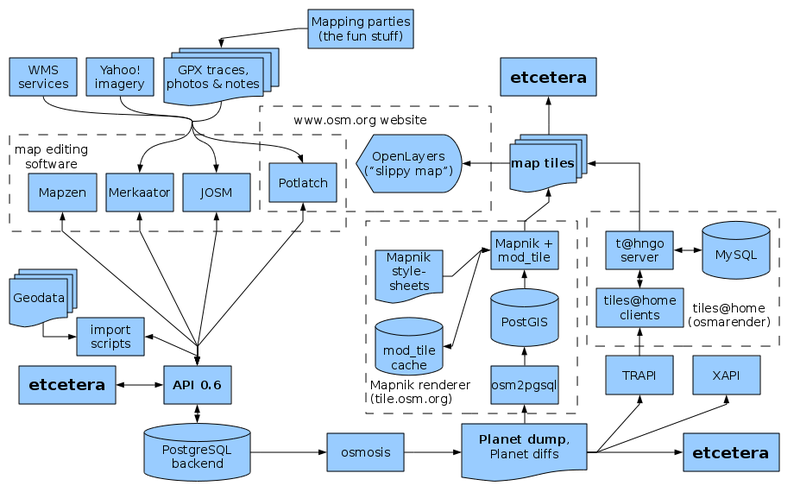
\includegraphics[width=0.85\textwidth]{images/800px-OSM_Components.png}
	\caption{Overview of OpenStreetMap's architecture.}
	\label{fig:osm-overview}
\scriptsize Source:\url{http://wiki.openstreetmap.org/w/images/1/15/OSM_Components.png} as of 2011 Apr 27th
\end{figure*}

To manage those datastructures, an infrastructure evolved encompassing multiple map editing tools, tile renderers, and data sources, as shown in Figure~\ref{fig:osm-overview}.

The data is stored in a relational database (PostgreSQL backend).
It can be accessed, queried and edited by using a REST API, which basically uses HTTP GET, PUT and DELETE requests with XML payload (similar to the example shown in Listing~\ref{lst:osc}).
The data is also published as complete dumps of the database in such an XML format on a weekly basis.
It currently accounts for more than 16GB of Bzip2 compressed data.
In minutely, hourly and daily intervals the project additionally publishes changesets, which can be used to synchronize a local deployment of the data with the OSM database.
The dumps as well as the changesets can be processed with the \emph{Osmosis} tool.

OpenStreetMap's community has build different authoring interfaces. These include the online editor \textit{Potlatch}, which is
implemented in Flash and accessible directly via the edit tab at the OSM map view, as well as the desktop applications \textit{JOSM}, \textit{Merkaartor} and \textit{Mapzen}. The editors use complementary external services and data such as \textit{Yahoo! satellite imagery} or \textit{Web Map Services} (WMS).
Additionally, users can upload GPS traces which serve as raw material for modelling the map.
Two different rendering services are offered for the rendering of raster maps on different zoom levels.
With \textit{Tiles@home}, the performance-intense rendering tasks are dispatched to idle machines of community members; thus achieving timeliness.
The \textit{Mapnik} renderer, in turn, operates on a central tile server and re-renders tiles only in certain intervals.

\begin{table*}[thb]
	\centering
		\begin{tabular}{lrrrr}
\textbf{Category} & \textbf{June 2009} & \textbf{April 2010} & \textbf{May 2011} & \textbf{Growth (past two years)} \\
\hline
Users (Thousands)	& 127 & 261 & 397 & + 213\% \\
Uploaded GPS points	(Millions) & 915 & 1500 & 2298 & + 151\% \\
Nodes (Millions)	& 374 & 600 & 1073 & + 187\% \\
Ways (Millions)	& 30 & 48 & 92 & + 207\% \\
% Relations	& 136,245 & ~300 & 6\% \\			
		\end{tabular}
% Quellen:
% 2009: http://jens-lehmann.org/files/2009/linkedgeodata_iswc.pdf
% 2010: http://aksw.org/files/claus_stadler__linkedgeodata__semantisch_vernetzte_geodaten.pdf
% 2011 (aktuell): http://www.openstreetmap.org/stats/data_stats.html
	\caption{OpenStreetMap statistics 2009 - 2011.\\(Obtained from \url{http://www.openstreetmap.org/stats/data_stats.html} at the specified months.)}
	\label{tab:OSMStatistics}
\end{table*}

Since the use of tags and values is not restricted, but governed by an agile community process, it is important to obtain an overview on emerging tags and tag values possibly specific to a certain region.
Services such as TagWatch\footnote{\url{http://tagwatch.stoecker.eu/}} periodically compute tag statistics for different areas.
In order for the data to be machine interpretable, as for instance for map rendering, contributors must follow certain editing standards and conventions\footnote{\url{http://wiki.openstreetmap.org/wiki/Map_Features}}.

Currently, OSM is in the process of switching from the Creative Commons CC-BY-SA license to the Open Database License\footnote{\url{http://www.opendatacommons.org/licenses/odbl/}}.
The term \textit{Volunteered Geographic Information} (VGI) was coined~\cite{michael2007citizens} for the harnessing of tools to create, assemble, and disseminate geographic data provided voluntarily by individuals -- with OSM being a driving force behind VGI.
% In any case, the data is freely available and is published as weekly full dumps. % Jens: wurde schon vorher gesagt
%Furthermore, changesets are provided on a minutely, hourly, and daily basis. % Jens: wurde schon vorher gesagt
% These datasets form the basis for LinkedGeoData.

The growth of the OpenStreetMap data has been enormous (cf. Table~\ref{tab:OSMStatistics}):
Since the founding in July 2004 until now, more than one billion nodes, about 90 million ways and close to 1 million relations have been contributed by the users\footnote{\url{http://www.openstreetmap.org/stats/data_stats.html}, retrieved 2011 May 2nd}.
Some of the data was imported form public domain datasources such as TIGER\footnote{\url{http://www.census.gov/geo/www/tiger}} for US, AND Automotive Navigation Data\footnote{\url{http://www.and.com/}} for The Netherlands, and GeoBase data from the Canadian government\footnote{\url{http://www.geobase.ca}}.

%\section{LinkedGeoData Overview}
\section{Architecture}
\label{sec:architecture}

The goal of the LinkedGeoData the project is to contribute rich, open, and integrated geographical data to the Semantic Web using OpenStreetMap as its base.
This is analogous to the well known DBpedia project, which follows a similar approach based on Wikipedia.
The necessary work for reaching this goal comprises the conversion of OSM data to RDF, the interlinking with other knowledge bases, the dissemination of the resulting data, and keeping the datasets up-to-date.
In this section, we give an overview of the LinkedGeoData architecture, followed by explanations of the details of the involved components in the next sections.

\begin{figure*}[htbp]
	\centering
%		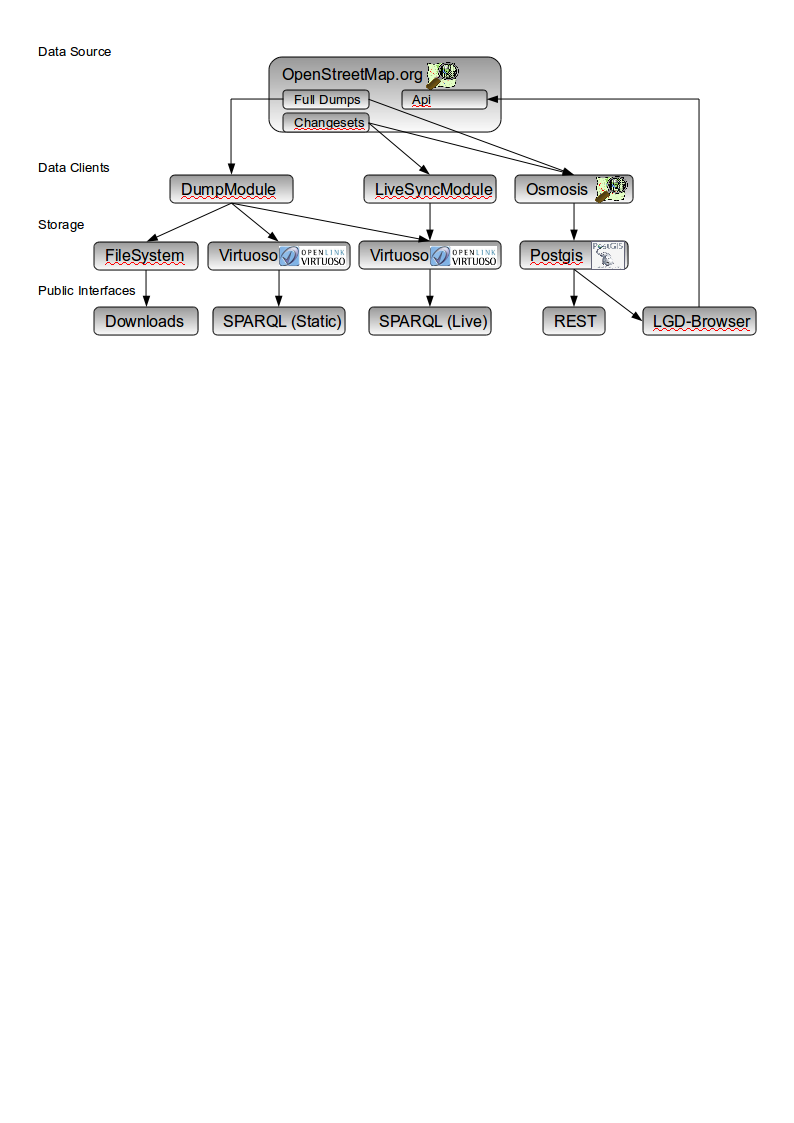
\includegraphics[width=\textwidth]{images/Architecture.png}
		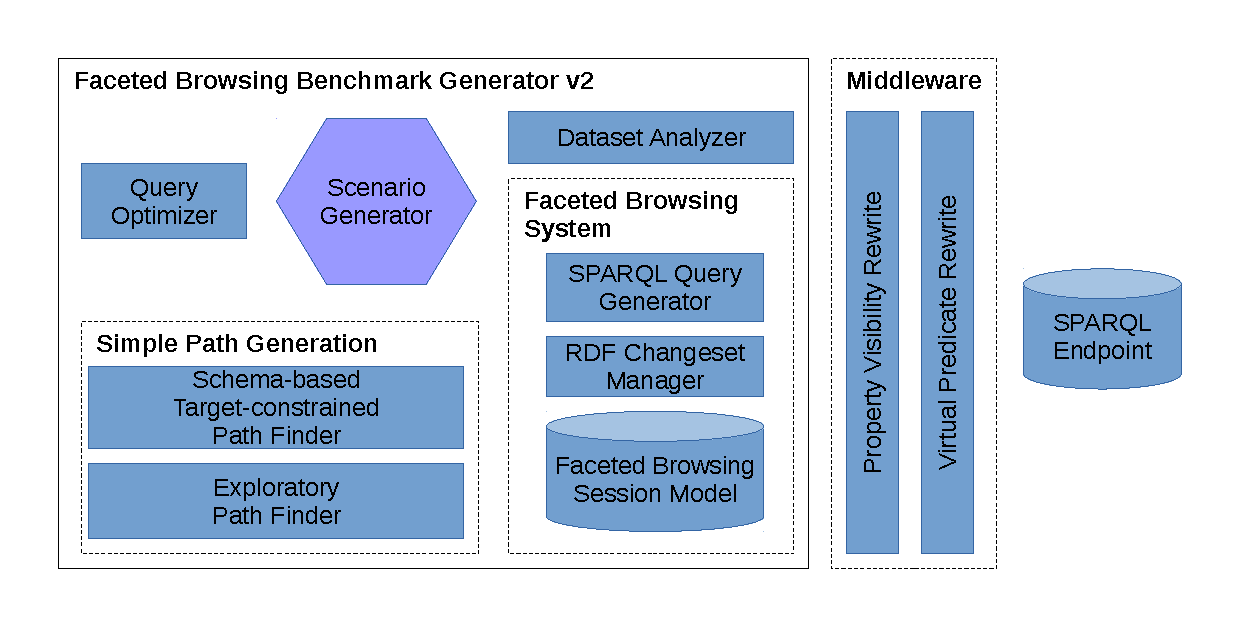
\includegraphics[width=0.85\textwidth]{images/Architecture.pdf}
	\caption{Overview of LinkedGeoData's architecture.}
	\label{fig:lgd-architecture}
\end{figure*}

%\subsection{Architecture}
The architecture of LinkedGeoData is illustrated in Figure~\ref{fig:lgd-architecture}.
It shows that the data from OpenStreetMap is processed on different routes:
The \emph{LGD Dump Module} converts an OSM planet file to RDF and loads the data
into a triple store. This data is then available via the
\emph{static SPARQL endpoint}.  A copy of that triple store serves as the initial basis
for the \emph{live SPARQL endpoint}.   
The \emph{LGD Live Sync Module} downloads minutely changesets from OpenStreetMap, and computes corresponding changesets on the RDF level in order to update that
triple store accordingly. 
By publishing these RDF changesets (see Section~\ref{sec:changeset-formats}), we enable data consumers to sync their own triple store with ours. Note, that not all OSM entities are loaded into the SPARQL endpoints due to performance reasons.
We offer SPARQL endpoints for the static and live version, because some use cases require up-to-date information whereas for others, it is more suitable that queries yield the same result over a longer period of time, e.g.~due to caching mechanisms.

For data access LinkedGeoData offers downloads, a REST API interface, Linked Data, and SPARQL endpoints.
The \emph{REST API} provides limited query capabilities for RDFized data
about \emph{all} nodes and ways of OpenStreetMap (relations are currently not
supported). It draws its data from a local replica of the OpenStreetMap PostGIS database.
The OpenStreetMap community developed a tool named 
\emph{Osmosis}\footnote{\url{http://wiki.openstreetmap.org/wiki/Osmosis}}, which
supports setting up such a database from a \textit{planet file} and applying
changesets to it. 
In future work, we aim for stronger support of spatial SPARQL queries by exposing PostGIS features via SPARQL.

% Jens: In obigen Text integriert. 
%The live SPARQL endpoint is synchronized with minutely updates from OSM, whereas the static one will contain all the data of the most recent LinkedGeoData release. Therefore, use cases which require up-to-date information as well as use cases where it is desirable for queries to yield the same results for a longer time span can be supported.
%Also, the static dump is more easy to set up from the downloads.
%Examples for uses of the live endpoint are the observation of an area in the
%search for new amenities or doing an evaluation on a particular area.

\section{RDF Mapping}
\label{sec:rdf_mapping}

In this section, we explain our approach to the generation of RDF triples from OpenStreetMap entities. 
Recall that all such OSM entities have a numeric ID and carry
information in form of values for predefined attributes and sets of tags.
The values for the predefined attributes, such as the version, the contributing
user, and timestamp are static and can also be seen as tags.

We generate URIs for nodes and ways according to the pattern
\verb=lgd:node<id>= and \verb=lgd:way<id>=, respectively.\footnote{See Appendix~\ref{sec:prefixes} for prefix declarations.} The resource
corresponding to a way's list of nodes is \verb=lgd:way<id>/nodes=.

These URIs are non-information resources, i.e. they represent
real-word entities. As such, stating that a resource corresponding to a pub
was created by a building company would be correct, however stating that it was
created with the map editor ``JOSM'' would be wrong.
In general, there are two possible solutions to permit both kinds of
statements: a) introduce distinct URIs for each of the two different
meanings, b) make use of annotation properties, which are intended for this purpose and do not have any logical implications. 
We chose the latter approach, because it avoids doubling the number of resources and keeps the data simple.
% for two reasons: Firstly it avoids doubling the number of resources, and secondly it keeps the data more simple. \todo{J

Our tag mapping approach is based on the assumption that each tag can be mapped in isolation, i.e.~without taking other possibly existing tags into account.
For example, entities with the tag \texttt{(amenity, school)} become instances of \texttt{lgdo:School}. 
Note, that this approach does not support more complex rules such as mapping all entities having both tags \texttt{(amenity, place\_of\_worship)} and \texttt{(religion, christian)} to e.g. \texttt{lgdo:Church}.
Therefore, the generated RDF structures are very close to the structure in OpenStreetMap.

We now specify the mapping process.
A \emph{tag mapper} is an object for generating RDF from tags.
It consists of a \emph{tag pattern} that specifies what tags to match,
and a \emph{transformation function} for generating the RDF.

Tag patterns can 1) match a specific key-value pair, such as \texttt{(amenity, school)}, 2) match all tags with a certain key (regardless of the values), e.g. \texttt{(tourism, *)}, or 3) match every tag. 
More specific patterns take precedence, e.g.~a matching pattern in category 1 overwrites matching patterns in category 2 and 3.
% A more concrete pattern implicitly takes precedence over less concrete patterns. This means, that the rule that matches every tag is only applied if no other rule matches.

We implemented the following four tag mappers:
\begin{itemize}
  \item \emph{Resource}: Maps a tag to a specific property and
  object, where both must be URIs. Therefore it can be used for mapping to
  both object properties and classes. In the latter case the property
  has to be set to \texttt{rdf:type}.
  Examples are \emph{(religion, christian)} and \emph{(amenity, school)} which
  are mapped to \emph{lgdo:religion lgdo:christian} and
  \emph{rdf:type lgdo:School}, respectively.
  \item \emph{Text}: Treats a tag's value as a plain literal. For example
  \emph{(note, nice view)}.
  \item \emph{Datatype}: Interpret a value e.g. \emph{(seats, 4)} with regard
  to a specific datatype.
  \item \emph{Language}: A mapper for tags whose key contains a
  language, such as \texttt{name:en}.
\end{itemize}

All of these mappings are implemented as Java classes, whose instances are
configured with an XML snippet. Listing~\ref{lst:tag-mapping} shows an example
of a configuration of a resource tag mapper that is interpreted as
follows: The 'simple' in the name reflects our limitation that tags are being
mapped in isolation. The mapping rule is applied to every entity that has a tag
matching the pattern \texttt{(religion,*)}.  The element \emph{objectAsPrefix} 
controls whether a tag's value should be appended to the value given as the object.
So in this case, a tag, such as \texttt{(religion, hindi)}, is mapped to the
predicate \texttt{lgdo:religion} and object \texttt{lgdo:hindi}.
The element \emph{describesOSMEntity} specifies whether the resulting RDF
describes a real world entity's representation on OpenStreetMap or the entity
itself. Therefore, it determines whether a mapping's property
should become an instance of \emph{owl:AnnotationProperty}.

The text- and datatype tag mappers are both similar to the resource tag
mapper, except that they map tag values to objects that are plain or typed
literals, respectively. Therefore the language and datatype of these mappers can
be set to a constant in their configuration.


The language tag mapper is used for mapping tag values to plain
literals with language tags inferred from the tags' keys. For instance
\emph{(name:en, Vienna)} would become \emph{(rdfs:label, ``Vienna''@en)}.
The key of its tag-pattern must be a regular expression containing a group for
matching the language, such as \verb=name:([^:]+)=. Every match for this
group is then cross checked against a list of known languages. This avoids for
example matching 'alt' as a language from the key
\emph{name:alt} for alternative names.

\begin{scriptsize}
\begin{lstlisting}[label=lst:tag-mapping, language=XML, caption=Example of a mapping declaration.]
<SimpleResourceTagMapper>
  <property>
    http://linkedgeodata.org/ontology/religion
  </property>
  <tagPattern>
    <key>religion</key>
  </tagPattern>
  <describesOSMEntity>false</describesOSMEntity>
  <objectAsPrefix>true</objectAsPrefix>
  <object>
    http://linkedgeodata.org/ontology/
  </object>
</SimpleResourceTagMapper>
\end{lstlisting}
\end{scriptsize}

This approach makes it possible to add new mappings that require more complex
processing easy. For example, a future tag mapper could extract the values of
\texttt{opening\_hours} tags (used ~60K times on nodes) and generate RDF in the
\textit{Good Relations}\footnote{\url{http://www.heppnetz.de/projects/goodrelations/}} vocabulary.

\subsection{The LinkedGeoData Ontology}
Based on the OpenStreetMap tags, we derived a lightweight OWL
ontology\footnote{The complete ontology is available at \url{http://linkedgeodata.org/ontology/}}.
A depiction of an excerpt in shown
in Figure~\ref{fig:ontology-excerpt}.
\begin{figure}[htbp]
	\centering
%		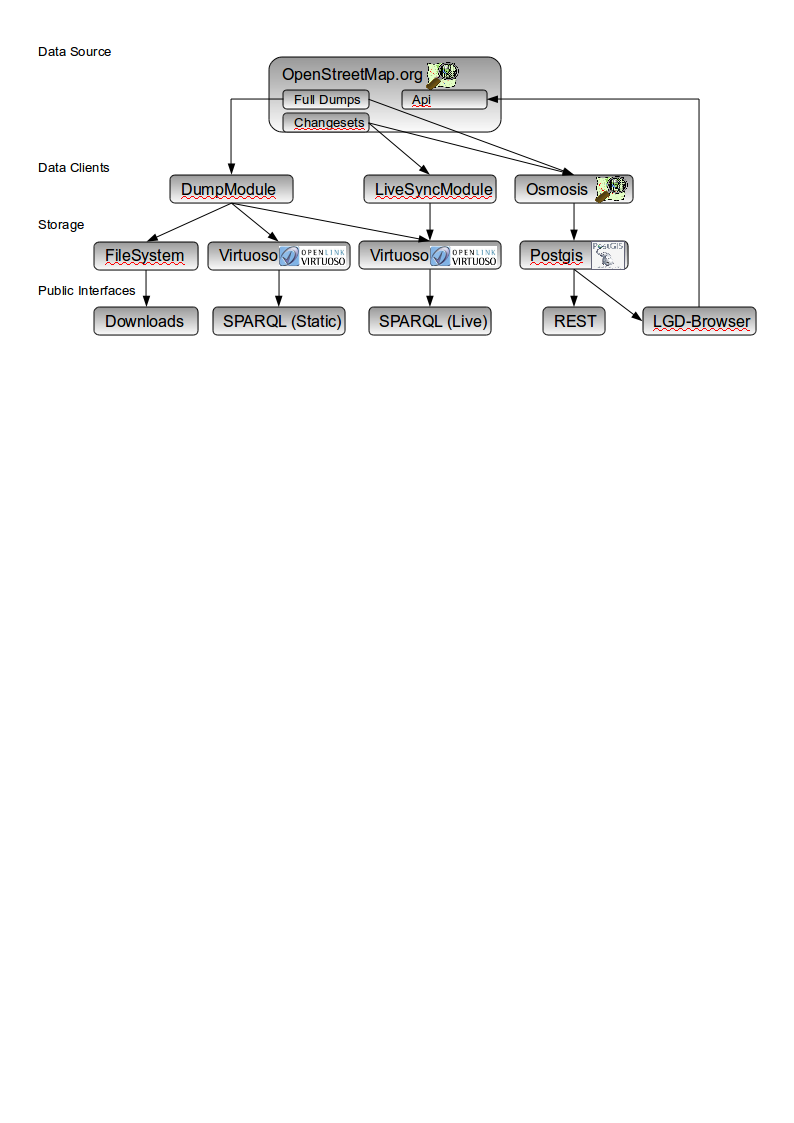
\includegraphics[width=\textwidth]{images/Architecture.png}
		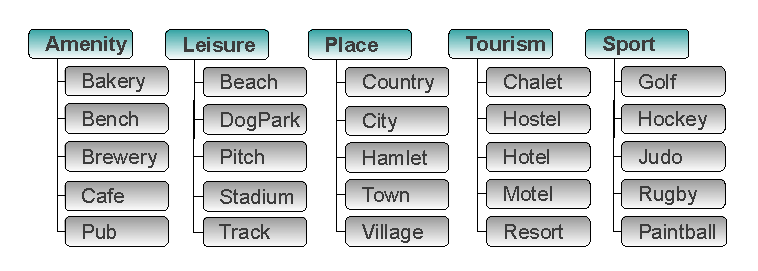
\includegraphics[width=0.5\textwidth]{images/OntologyExcerpt.pdf}
	\caption{An excerpt of the LinkedGeoData ontology.
	More classes and subclasses exist in the actual version.}
	\label{fig:ontology-excerpt}
\end{figure}
%\footnote{The full ontology is available at
%\url{http://linkedgeodata.org/ontology/}}

The process of creating it is explained as follows:
Subclass relationships are inferred from resource tag mapper configurations: If
there are two tag patterns for \emph{(tag1, tag2)} and \emph{(tag1, *)}, which
use the \verb|rdf:type| property, then the object of the first tag pattern
becomes a subclass of the second tag pattern. For example,
Listing~\ref{lst:tag-mapping-subclass} shows an example of such tag mappings
for the \emph{(amenity, restaurant)} and \emph{(amenity, *)} tag patterns.

%\todo{Jens: Habe es in zwei Saetze zerlegt und vereinfacht. Bitte pruefen, ob es dennoch korrekt ist. Inbesondere koennte man erwaehnen, warum das \emph{(amenity, *)} ueberhaupt notwendig ist, d.h. warum es nicht reicht das tag2 auf eine Klasse gemappt wird.}
% If for a specific tag-pattern, such as \emph{(amenity, restaurant)}, there exists less specific one, such as \emph{(amenity, *)}, and both corresponding mapping rules map entities to instances of classes, such as \emph{Amenity} and \emph{Restaurant}, then the class of of the specific tag-pattern becomes a sub-class of the general one. In this example we would infer that \emph{Restaurant} is a subclass of \emph{Amenity}.

\begin{scriptsize}
\begin{lstlisting}[label=lst:tag-mapping-subclass, language=XML, caption=Subclass relationship example.]
<SimpleResourceTagMapper>
  <property>rdf:type</property>
  <tagPattern>
    <key>amenity</key>
  </tagPattern>
  <describesOSMEntity>false</describesOSMEntity>
  <objectAsPrefix>false</objectAsPrefix>
  <object>
    http://linkedgeodata.org/ontology/Amenity
  </object>
</SimpleResourceTagMapper>
<SimpleResourceTagMapper>
  <property>rdf:type</property>
  <tagPattern>
    <key>amenity</key>
    <value>restaurant</value>
  </tagPattern>
  <describesOSMEntity>false</describesOSMEntity>
  <objectAsPrefix>false</objectAsPrefix>
  <object>
    http://linkedgeodata.org/ontology/Restaurant
  </object>
</SimpleResourceTagMapper>
\end{lstlisting}
\end{scriptsize}

In order to determine datatype properties, we scanned all OSM tags for those that had keys for which the majority of values could be parsed as boolean, integer, and float datatype values. 
In order to deal with dirtiness in tag usage, we applied the following two criteria on the relative and absolute error rate:
\begin{itemize}
  \item At least 99\% of a key's values must succeed to parse.
  \item The absolute number of errors must not exceed 5000.
\end{itemize}
The most specific datatype meeting these criteria then became the range of the key's corresponding property. 
If a datatype was determined, all invalid values were omitted in the RDF output.

Object properties were identified as follows:
Intuitively, tags that might be suitable for being mapped to object properties meet the condition, that a low number of distinct values covers most its uses. 
However, this heuristic only serves as an indicator for tag candidates, as the final choice may be subjective.
For instance, only 7 distinct values for the key \emph{note:ja} are used in more than 99\% of almost 3.5mio tags. 
However, since the tag corresponds to a note, we considered a datatype property to be the right choice.
%\todo{Beispiel fuer object property angeben.}
An example for an object property is \emph{lgdo:religion}, which links to
resources in the \emph{lgdo} namespace, such as \emph{christian}, \emph{muslim},
and \emph{buddhist}.
Another example is \emph{lgdo:wheelchair}, which specifies the extent of
wheelchair accessibility, using resources mainly corresponding to the
values \emph{yes}, \emph{no}, \emph{limited}, and \emph{unknown}.
Using those heuristics, we could generate seed mappings for OpenStreetMap, which were then manually reviewed and refined.


\subsection{Multilingual labels and icons}
The OpenStreetMap community conducts various internationalization efforts, such as for
their website, their map editing tools, and their search engine.
Some of these efforts are coordinated on \emph{TranslateWiki}, which describes
itself as ``a localisation platform for translation communities, language
communities, and free and open source
projects.''\footnote{\url{http://translatewiki.net}} Essentially, this wiki
enables contributors to assign texts in multiple languages to keys.
The group \emph{OpenStreetMap - Website} defines 1441 keys, and has a 100\%
translation coverage for 13 languages and 12 more languages with a coverage of
more than 90\%\footnote{\url{http://translatewiki.net/wiki/Translating:OpenStreetMap/stats/trunk} retrieved 5th May 2011.}.
They keys with the prefix \emph{geocoder.search\_osm\_nominatim.prefix}
correspond to human readable representations of individual tags, and as such
form a rich, multilingual, and high quality source of labels for classes,
properties, and instances, which we integrated into the LinkedGeoData ontology.

These labels could serve as a basis for answering queries posed in different
languages: For a query such as ``Bakeries in Munich'' and its German
equivalent ``B\"{a}ckereien in M\"{u}nchen'', the search words could be mapped
to corresponding classes and instances from the LinkedGeoData knowledge
base.
A system already capable of processing such types of queries is described
in~\cite{spirit}.


As for icons, there exists a \textit{CC-0} licensed collection of 307 SVG map
icons (of which 47 icons are alternative versions) from SJJB
Management.\footnote{\url{http://www.sjjb.co.uk/mapicons/} retrieved 6th April 2011}
Currently the LinkedGeoData ontology associates 90 of them with classes,
using the annotation property \emph{lgdo:schemaIcon}.
The icons themselves are re-published on our server. 
They simplify the creation of visually appealing LGD based applications and mashups.

\section{Data Access}
\label{sec:data_access}

As briefly mentioned in Section~\ref{sec:architecture}, we provide several ways to access LinkedGeoData:
\begin{itemize}
 \item dataset downloads (HTML download table\footnote{\url{http://linkedgeodata.org/Datasets}} and actual files\footnote{\url{http://downloads.linkedgeodata.org}}), including live sync changesets relative to the latest release\footnote{\url{http://downloads.linkedgeodata.org/releases/latest/changesets/}} (explained in Section~\ref{sec:synchronization})
 \item a static SPARQL endpoint\footnote{\url{http://linkedgeodata.org/sparql}}
 \item a live SPARQL endpoint\footnote{\url{http://live.linkedgeodata.org/sparql}}
 \item Linked Data via 303 content negotation (RDF/XML, Turtle, N-Triples, HTML formats supported)
 \item a REST API
\end{itemize}

We first show an example data excerpt and then explain the REST API.

\subsection{Data example}
In Listing~\ref{lst:lgd-dataset-example}, we give a brief example on how the data in LinkedGeoData looks like.
The whole type hierarchy is already inferred, as it is being done in DBpedia, i.e.~\verb|rdf:type| relations to all super classes are asserted.
The \emph{lgdo:directType} property was added on request in order for applications to easily determine the most specific types of instances.
For every way, there exists a triple that contains the positions of all nodes.
For open and closed ways the predicates are \emph{georss:linestring} and \emph{georss:polygon}, respectively.
Note that this interpretation is not always correct, as in the general case closed ways have to be interpreted in the context of the ways' tags in order to determine whether the enclosed area counts to the way or not.
All nodes belonging to a way are kept in an RDF sequence.
In the SPARQL endpoints, geographical coordinates are represented as point geometries that are typed with \emph{virtrdf:Geometry}.
OpenLink's Virtuoso\footnote{\url{http://virtuoso.openlinksw.com}} enterprise
edition database system automatically indexes such points in an R-tree.

\begin{scriptsize}
\begin{lstlisting}[label=lst:lgd-dataset-example, language=ttl, caption=Example dataset in Turtle syntax.]
lgd:way4009992
  a            lgdo:Tennis, lgdo:Sport, lgdo:Way;
  lgdo:directType  lgdo:Tennis;
  lgdo:contributor lgd:user2274;
  lgdo:hasNodes    <http://.../way4009992/nodes>;
  georss:polygon  "52.1523857 -1.026259
                     52.1522675 -1.0264068 ..." .
<http://.../way4009992/nodes>
  a       rdf:Seq;
  rdf:_1  lgd:node21179607;
  rdf:_2  lgd:node21179608;
  ... .
lgd:node21179607 geo:geometry
  "POINT(-1.02626 52.1524)"^^virtrdf:Geometry
\end{lstlisting}
\end{scriptsize}

\subsection{The REST API}

\begin{figure}[htbp]
	\centering
%		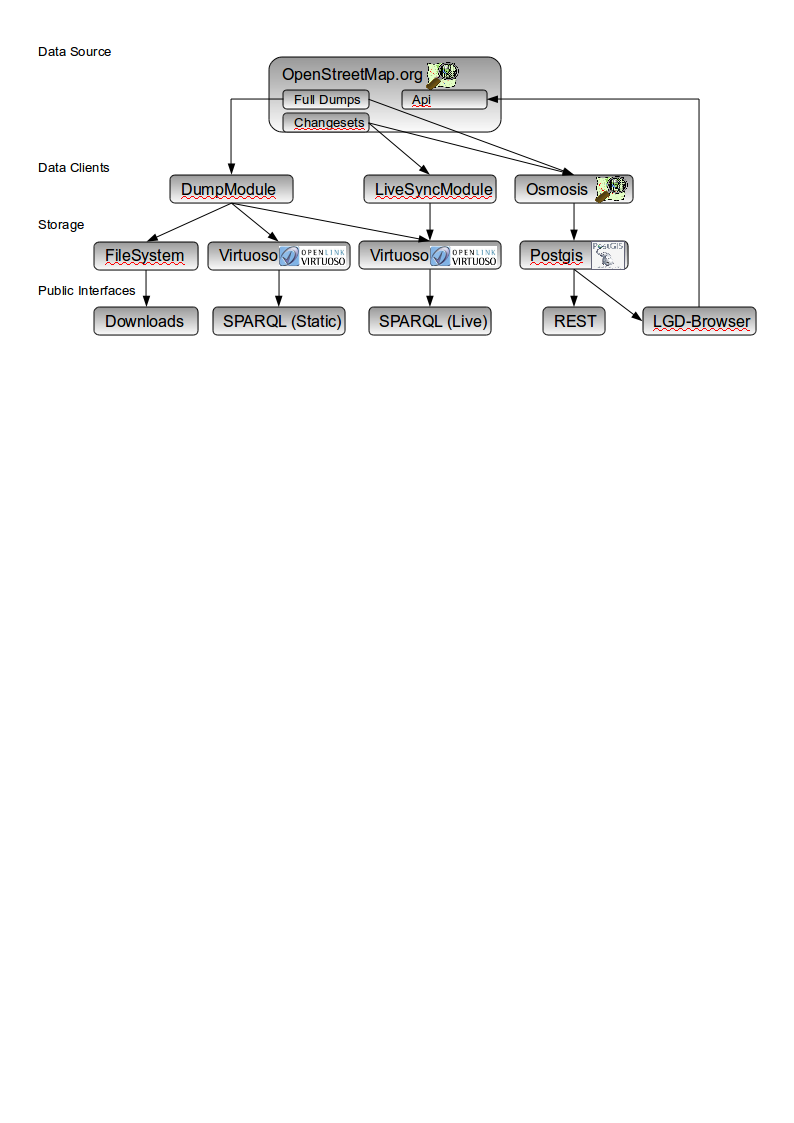
\includegraphics[width=\textwidth]{images/Architecture.png}
		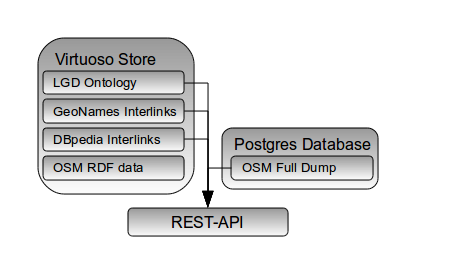
\includegraphics[width=0.4\textwidth]{images/RestArchitecture.png}
	\caption{Data Sources of the REST API.}
	\label{fig:rest-api-architecture}
\end{figure}

%In this section we introduce the LinkedGeoData REST API.
The LinkedGeoData REST API gives access to all of OpenStreetMap's nodes and ways.
It offers a set of methods that all have in common that they return RDF for responses. 
Each call to the REST API can be combined with content negotiation to format these responses as RDF/XML, N-Triples, or Turtle.
The API is backed by two things: on the one hand there is a PostGIS database
that is loaded with an OSM planet file and which is updated with minutely OSM changesets. On the other hand, the data for the ontology and interlinking is drawn from the SPARQL endpoints, as depicted in Figure~\ref{fig:rest-api-architecture}.

\begin{table*}[htb]
\begin{tabular}{ll}
\toprule
URLs relative to \url{http://linkedgeodata.org/triplify/near/} & Description \\
(General syntax and specific example) \\
\midrule
% Jens: würde ich rausnehmen, da als Linked Data im Text beschrieben
%\url{ontology} & Retrieves the whole ontology \\
%\url{node264695865} & Retrieves information about a specific node. \\
%\url{way4564184} & Same for ways \\
\url{<latmin>-<latmax>,<lonmin>-<lonmax>} & Resources located in the given rectangle. \\
\url{51.02-51.04,13.72-13.74}  \\
\url{<lat>,<lon>/<radius>} & Resources located in specified radius in meters from the given point. \\
\url{51.02-51.04/1000}  \\
\url{<lat>,<lon>/<radius>/class/<classname>} & Resources in specified radius belonging to the given class. \\
\url{51.033333,13.733333/1000/class/PlaceOfWorship} \\
\url{<lat>,<lon>/<radius>/class/} & Resources in specified radius, belonging to the given class with a \\
\url{<classname>/label/<lang>/contains/<label>} & label in the specified language containing a specific string. \\
\url{.../class/Amenity/label/en/contains/flower} \\ 
%\url{near/.../class/Shop/label/contains/any/flower} & Same as above,
%additionally instances must be of class \texttt{lgdo:Shop} \\
% & and their label must contain the substring ``flower'' in any language.
\bottomrule
\end{tabular}
\caption{Excerpt of the methods supported by the LGD REST API.}
\label{tab:rest-api-methods}
\end{table*}

An excerpt of the available methods is given in Table~\ref{tab:rest-api-methods}.
In general, the REST API returns a set of spatial entities along with their RDF descriptions, which can be filtered in numerous ways:
\begin{itemize}
 \item by area: Either a circular or rectangular area can be selected via WGS84 coordinates.
 \item by class: Returned resources can be restricted to a single LinkedGeoData class.
 \item by name (\verb|rdfs:label|): It can be set whether returned points should contain or start with a certain string. Furthermore, it can be specified whether name search should be case sensitive and whether only names with a particular language tag should be considered.
\end{itemize}
Using area and label search combined with class restrictions were the most requested features in applications, which is why we provide them in the REST interface.
The main purpose of the REST API is to lower the entry barrier for data consumers and to internally optimise the performance of the most commonly used queries.

\section{Interlinking}
\label{sec:interlinking}

% Jens: Habe das in den Anhang verschoben.
\begin{comment}
\tymin20pt
\begin{table}[ht]\label{tab:prefixes}
\begin{tabulary}{0.5\textwidth}{LL}
\toprule
prefix	&URL\\
\midrule
%lgd	&\url{http://linkedgeodata.org/}\\
lgdo	&\url{http://linkedgeodata.org/ontology/}\\
%lgdt	&\url{http://linkedgeodata.org/triplify/}\\
gn	&\url{http://www.geonames.org/ontology\#}\\
wgs84 	&\url{http://www.w3.org/2003/01/geo/wgs84_pos\#}\\ 
foa	&\url{http://www.fao.org/countryprofiles/geoinfo/geopolitical/resource/}\\
\bottomrule
\end{tabulary}
\caption{The prefixes used in this section}
\end{table}
\end{comment}

In this section, the interlinking between \emph{LinkedGeoData},
\emph{DBpedia}, \emph{GeoNames} and the
\emph{Food and Agriculture Organization of the United Nations (FOA)} is
described.
In all cases, we first manually aligned the classes of these
knowledge bases with classes from LinkedGeoData on an best effort basis.
The interlinking is then done on a per-class basis, where all instances of a set
of classes of LGD are matched with all instances of a set of classes of another data source using labels and spatial information. As an example, cities in LGD
and DBpedia are matched between all instances of \nolinkurl{lgdo:City}, \nolinkurl{lgdo:Town}, \nolinkurl{lgdo:Village} and
\nolinkurl{lgdo:Hamlet} on one side and \nolinkurl{dbo:Settlement} on the other.
The interlinking is performed using the tools SILK~\cite{silk} and
LIMES~\cite{limes}, which use the static SPARQL endpoint as the backend. As
Virtuoso's index support for geometries is limited to points, we needed to constrain the interlinking to
LinkedGeoData nodes. An overview of triple stores supporting complex
geometries is given in Section~\ref{sec:geo-semantic-web}.

%In contrast, a LinkedGeoData way does not have a position itself, but has a
%potentially high number of nodes, each of which has a WGS84 position.
It should be noted, that many ways in OpenStreetMap have reference
points, e.g.~characteristic points for a given way. Those reference points
are not necessarily located in the geometric center of a way, but represent
a typical point by OSM community consensus.

%instead may contain millions of points describing the path 
%or outline of a geographical feature and is thus unsuitable for this kind of matching.
\iffalse %rausgenommen, weil das schon in der Statistik drin ist
\begin{table}[hb]
\begin{tabular}{lr}
\toprule
class				&number of instances\\
\midrule
City $\cup$ Town $\cup$ Village $\cup$ Hamlet 	&\val{818893}\\
%City $\cup$ Town $\cup$ Village 		&\val{544890}\\
School						&\val{331242}\\
Building					&\val{257893}\\
Park 						&\val{151833}\\
Peak						&\val{148580}\\
Waterway 					&\val{90455}\\
Island						&\val{51472}\\
River 						&\val{2651}\\
Country 					&\val{235}\\
\bottomrule
\end{tabular}
\caption{Some LinkedGeoDatas classes, not counting transitive membership.}
\label{tab:geonames-featureclasses}
\end{table}
\fi

For each class-mapping, a link specification is created and executed using the \emph{Silk Link Discovery Framework} \cite{silk}.
The link specs usually include a metric, which is a linear classifier depending on the labels and the geographic distance,
which can be calculated from the values of \nolinkurl{wgs84:lat} and \nolinkurl{wgs84:long} properties which are provided by all considered data sources.
By combining classification, naming and spatial features, we are able to obtain very precise interlinking heuristics as shown later.

We used the following matching criterion, which we explain in detail below:
\[\frac{2}{3} s(a,b) + \frac{1}{3} g_c(a,b) > 0.95\]

\begin{itemize}
 \item $a$ and $b$ are the resources to be compared
 \item $s(a,b)$ is a the \emph{Jaro-Winkler distance}~\cite{WIN99}, between the
 labels of $a$ and $b$. If there are multiple labels, the pair with the maximum score is chosen, ignoring the language-tag.
While this could cause false links in the special case that the label of a
resource in one language is very similar to the label of a resource in a
different language, this type of error was not found in our evaluation.
%between pair of different geographical features $A$ and $B$, where the name of one in one language
%is very similar to name of the other in another language, this particular error was not found in our evaluation.
An advantage of this approach is that it works for several languages even if the proper language tags are actually missing.
% On the other hand, this approach can make use of the many labels without a language tag and is simple to implement in \emph{SILK}.
 \item $c$ is the maximum distance that two points describing the same object are reasonably expected to differ.
While a good value for $c$ is easily chosen in some cases (a shop does not span more than a few hundred meters), it is nontrivial in cases of large variances
in size such as in cities, mountains or islands.
The value of $c$ varies greatly between classes and is explained by the choice of reference points, which can differ in each of the considered knowledge bases.
 \item $g_c(a,b) =
\begin{cases}
0 & d > c \\
1/(1+e^{-12d'+6}) & otherwise
\end{cases}$
In this formula, $d$ is the distance between $a$ and $b$. The distance is approximated by the \emph{haversine formula}, which uses a spherical model of the earth.
We then define $d' = 1 - d/c$ which is a linear function with a value of zero at distance $d=c$ and one for $d=0$.
In order to not punish a slight discrepancy between two points as much as a linear function would, $d'$ is not used directly.
Instead, we employ a scaled logistic curve. The remaining parameters are adjusted such that two objects at distance $c$ with exactly the same labels almost exactly matches the threshold of 0.95 in the formula above, which is the intended meaning of the parameter $c$.
\end{itemize}

%Because of the chosen threshold of \val{0.95} however, two entities with a distance of exactly $c$ would not be considered a match even 
%if their labels were exactly equal.
%This is alleviated by using $c' = 4c$ instead of $c$,
%because in this case $d' = 1 - \frac{c}{4c} = \frac{3}{4}$ and $1/(1+e^{-12\frac{3}{4}+6}) \approx \val{0.952}$.
%This means that as long as the string similarity value is above $\val{0.95}$, a distance of $c$ is guaranteed to be a match.

%\footnotetext{$2/3+1/3*x = \val{0.95}$}
\iffalse
2/3+1/3*x = 0.95
1/3 x = 0.95 -2/3
x = 0.95*3-2 = 3-2-0.05*3 = 1 0.15 = 0.85
\fi
\subsection{Interlinking with DBpedia}
Since the initial interlinking between LinkedGeoData and DBpedia as described in \cite{linkedgeodata} in 2009, both knowledge bases have
grown and changed significantly, resulting in the need of a new interlinking as well as an exhaustive re-evaluation of the quality of the interlinks.
Table~\ref{tab:linkedgeodata-dbpedia-matching} shows the created class-mappings and the size of the linksets and their estimated precisions.
The links were manually evaluated with a random sample of 250 instances each. In cases where the number of links is smaller
than or only slightly higher than 250 as in the case of the universities, all of the instances were evaluated.
\tymin=1pt
%\tymax=100pt
\begin{table}[ht]
\caption{LinkedGeoData-DBpedia linksets.}
\label{tab:linkedgeodata-dbpedia-matching}
\begin{threeparttable}
\begin{tabulary}{0.502\textwidth}{LRLRRRR}
\toprule
DBpedia	class		&instances	&LGD equivalent		&c in km			&nodes		&links		&precision\\
\midrule
Airport			&9520		&Aerodrome		&2.5	&43734	&8404	&1.0\\
Settlement 		&239630		&several\tnote{1}			&0.1	&620387	&88377	&1.0\\
Country			&2505\tnote{2}	&Country		&1000	&231	&222	&0.991\\
%x			&	&				&				&		&\\
University		&11607	&University			&2.5	&17715	&268	&1.0\\
Stadium			&5539	&Stadium			&1	&13001	&133	&1.0\\
School			&22686	&School				&1	&262566	&2470	&1.0\\
Island			&2371	&Island				&100	&31121	&449	&1.0\\
Mountain		&8742	&Peak				&100	&177702	&3258	&0.992\\
\midrule
Overall			&302600	&				&			&1166457	&103581	&0.966\\
% Jens: too few links
% Lake			&\val{8221}	&Water				&\valunit{25}{km}			&\val{311}		&\val{0}	&\val{0.0}\\
% Jens: too few links
%River			&\val{18526}	&Waterway $\cup$ River		&\valunit{250}{km}			&\val{93106}		&\val{8}	&\val{1.0}\\
% old with valunit:
\iffalse
DBpedia	class		&instances	&LGD equivalent	&c in km			&nodes		&links		&precision\\
\midrule
Airport			&\val{9520}	&Aerodrome			&\val{2.5}	&\val{43734}	&\val{8404}	&\val{1.0}\\
Settlement 		&\val{239630}	&City $\cup$ Suburb $\cup$ Town $\cup$ Village
									&\val{0.1}	&\val{620387}	&\val{88377}	&\val{1.0}\\
Country			&\val{2505}\tnote{1}	&Country		&\val{1000}	&\val{231}	&\val{222}	&\val{0.991}\\
%x			&\val{}	&				&\val{}				&\val{}		&\val{}\\
University		&\val{11607}	&University			&\val{2.5}	&\val{17715}	&\val{268}	&\val{1.0}\\
Stadium			&\val{5539}	&Stadium			&\val{1}	&\val{13001}	&\val{133}	&\val{1.0}\\
School			&\val{22686}	&School				&\val{1}	&\val{262566}	&\val{2470}	&\val{1.0}\\
Island			&\val{2371}	&Island				&\val{100}	&\val{31121}	&\val{449}	&\val{1.0}\\
Mountain		&\val{8742}	&Peak				&\val{100}	&\val{177702}	&\val{3258}	&\val{0.992}\\
\fi
\bottomrule
\end{tabulary}
\begin{tablenotes}
\item [1] City $\cup$ Suburb $\cup$ Town $\cup$ Village
\item [2] The large number of countries is caused by former countries like \emph{Republic of Texas} and \emph{Inca Empire}.
\end{tablenotes}
\end{threeparttable}
\end{table}

%TODO: Konrad - Kapitel schreiben
%
%DBpedia, GeoNames + möglichst weitere wie z.B. Flughafen Codes o.ä. verlinken => LinkedGeoData sollte als Hub im GeoDaten-Web erscheinen 
%TODO Claus: Schemalinks publizieren (es ist nicht notwending die wieder aus den instanzen rauszufinden (reading group seite))

\subsection{Interlinking with GeoNames}
The GeoNames database contains over 10 million geographical names and has 7.5 million unique features.
It integrates sources such as the \emph{National Geospatial-Intelligence Agency's} (\emph{NGA}) and the \emph{U.S. Board on Geographic Names}.
While at the time of this writing there is no official SPARQL endpoint yet, an RDF-dump and an ontology are available.
The ontology is very flat, with only two layers of disjunctive classes, where the superclasses are called \emph{feature classes} and the subclasses \emph{feature codes}.
The feature codes are very detailed, for example there are 97 feature codes for the feature type \nolinkurl{T} (\emph{Peak}).
Linking GeoNames with LinkedGeoData makes these detailed features available to
LinkedGeoData. In addition to the steps used for linking LinkedGeoData with DBpedia, the labels (which are represented by the properties \nolinkurl{gn:name} and \nolinkurl{gn:alternateName} in GeoNames) are first transformed by removing all occurrences of the name of class of the instances (e.g. \emph{``city''}). This increases the string similarity score for pairs like (``Fananu'', ``Fananu Island'').
Again, 250 links per class were evaluated and the results are shown in
Table~\ref{tab:linkedgeodata-geonames-matching}.

\tymax=140pt
\begin{table*}[ht]
\begin{threeparttable}
\caption{Matching classes and created links between LGD and Geonames.}
\label{tab:linkedgeodata-geonames-matching}
\begin{tabulary}{\textwidth}{LRLRRRR}
%\begin{tabulary}{\textwidth}{LLRLLR}
\toprule
GeoNames feature class or code				&number of features	&LinkedGeoData class	&c		&number of nodes	&links	&precision\\
\midrule
PCL $\cup$ PCLD $\cup$ PCLF $\cup$ PCLI $\cup$ PCLIX $\cup$ PCLS
						&\val{237}		&Country			&\valunit{1000}{km}		&\val{235}		&\val{218}	&\val{0.995}\\

PRK						&\val{71764}		&Park				&\valunit{5}{km}		&\val{151833}		&\val{55648}	&\val{0.992}\\
PPL $\cup$ PPLA $\cup$ PPLA2 $\cup$ PPLA3 $\cup$ PPLA4 $\cup$ PPLC $\cup$ PPLF $\cup$ PPLG $\cup$ PPLL $\cup$ PPLQ $\cup$ PPLR $\cup$ PPLS $\cup$ PPLW
						&\val{2821405}		&Hamlet $\cup$ Village $\cup$ Town $\cup$ City	
													&\valunit{100}{km}\tnote{1}		&\val{818893}		&\val{34907}		&\val{0.984}\\
%S						&\val{1554654}		&Building							&\val{257893}	&\val{}	&\val{}\\
%T\tnote{1}					&\val{1014431}		&Peak				&\valunit{100}{km}		&\val{148580}		&\val{236711}	&\val{0.518}\\
%ISL						&\val{28189}		&Island				&\valunit{400}{m}		&\val{51472}		&\val{37399}	&\val{0.631}\\
SCH						&\val{224217}		&School				&\valunit{1}{km}		&\val{340039}		&\val{168545}	&\val{1.0}\\
PRK						&\val{72130}		&Park				&\valunit{5}{km}		&\val{157862}		&\val{55648}	&\val{0.992}\\
%T						&\val{1015114}		&Peak	&\val{177727}	&\val{236711}	&\val{}\\
% commented out, because it is not evaluated
%STM $\cup$ STMM $\cup$ STMC $\cup$ STMSB $\cup$ STRT $\cup$ STMIX $\cup$ STMA $\cup$ STMS $\cup$ STMB $\cup$ STMH $\cup$ STMX $\cup$ STMD $\cup$ STMQ $\cup$ STMI
%						&\val{833870}	&River $\cup$ Waterway	&\val{3233409}	&\valunit{1000}{km}		&\val{47101}	&\val{?\tnote{2}}\\			
STDM						&\val{753}		&Stadium			&\valunit{1}{km}		&\val{13001}		&\val{24}	&\val{1.0}\\
FRM $\cup$ FRMQ $\cup$ FRMS $\cup$ FRMT		&\val{207171}		&Farm				&\valunit{6000}{m}		&\val{3834}		&\val{54}	&\val{1.0}\\
AIRH $\cup$ AIRP $\cup$ AIRQ $\cup$ AIRB $\cup$ AIRF	&\val{32449}	&Airport $\cup$ Aerodrome $\cup$ Aerialway $\cup$ Aeroway
													&\valunit{10}{km}		&\val{175006}		&\val{21552}	&\val{1.0}\\
% not enough links													
% PKLT						&\val{119}		&Parking			&\valunit{1}{km}		&\val{494787}		&\val{1}	&\val{1.0}\\
MALL $\cup$ MKT					&\val{18240}		&Supermarket $\cup$ Shop $\cup$ Mall		
													&\valunit{1}{km}		&\val{572833}		&\val{59}	&\val{0.949}\\
TMPL $\cup$ CH $\cup$ CTRR			&\val{231678}		&PlaceOfWorship			&\valunit{1}{km}		&\val{352673}		&\val{201318}	&\val{0.976}\\
REST						&\val{1195}		&Restaurant			&\valunit{1}{km}		&\val{167293}		&\val{55}	&\val{1.0}\\
% not enough links
% GRVE						&\val{561}		&GraveYard			&\valunit{5}{km}		&\val{134371}		&\val{1}	&\val{1}\\
% not enough links
% DPOF						&\val{23}		&Fuel				&\valunit{1}{km}		&\val{124296}		&\val{1}	&\val{1}\\
HTL						&\val{82876}		&TourismHotel			&\valunit{200}{km}		&\val{63516}		&\val{2214}	&\val{0.958}\\
HSP						&\val{16606}		&Hospital			&\valunit{5}{km}		&\val{58095}		&\val{11032}	&\val{0.976}\\
% not enough links
%CTRM						&\val{51}		&MedicalCentre			&\valunit{5}{km}		&\val{69}		&\val{0}	&\\
PO						&\val{31244}		&PostOffice			&\valunit{1}{km}		&\val{50962}		&\val{20718}	&\val{1.0}\\
% not enough links
% PIER						&\val{296}		&Pier				&\valunit{1}{km}		&\val{45373}		&\val{5}	&\val{1.0}\\
GDN						&\val{380}		&Garden				&\valunit{1}{km}		&\val{35542}		&\val{11}	&\val{1.0}\\
PP						&\val{1209}		&Police				&\valunit{1}{km}		&\val{28363}		&\val{24}	&\val{1.0}\\
LIBR						&\val{10712}		&Library			&\valunit{1}{km}		&\val{25637}		&\val{9225}	&\val{1.0}\\
%PPLL $\cup$ PPLA3 $\cup$ PPLA $\cup$ PPLW $\cup$ PPL $\cup$ PPLR $\cup$ PPLA2 $\cup$ PPLA4 $\cup$ PPLG $\cup$ PPLS $\cup$ PPLF	&\val{2786506}	&Village $\cup$ Suburb $\cup$ City $\cup$ Town	&\val{589426}	&\val{}	&\val{}\\
SHRN						&\val{16379}		&Memorial			&\valunit{100}{m}		&\val{22613}		&\val{168}	&\val{1.0}\\
MUS						&\val{4409}		&TourismMuseum			&\valunit{2}{km}		&\val{21442}		&\val{3291}	&\val{0.996}\\
% not enough links
% RHSE						&\val{652}		&Shelter			&\valunit{2}{km}		&\val{20035}		&\val{0}	&\\
CLF						&\val{7668}		&Cliff				&\valunit{2}{km}		&\val{18738}		&\val{4414}	&\val{1.0}\\
UNIV						&\val{363}		&University			&\valunit{2}{km}		&\val{17715}		&\val{48}	&\val{0.896}\\
BAY						&\val{45230}		&Bay				&\valunit{5}{km}		&\val{16595}		&\val{14670}	&\val{1.0}\\
BCHS $\cup$ BCH					&\val{7533}		&Beach $\cup$ TourismBeach $\cup$ NaturalBeach	
													&\valunit{10}{km}		&\val{14129}		&\val{2028}	&\val{1.0}\\
% not enough links													
% BUSTP						&\val{346}		&BusStation $\cup$ Halt		&\valunit{1}{km}		&\val{24427}		&\val{0}	&\\
% not enough links
% GHSE						&\val{269}		&GuestHouse			&\valunit{1}{km}		&\val{10543}		&\val{3}	&\val{1.0}\\
CSTL						&\val{3615}		&Castle				&\valunit{2}{km}		&\val{8406}		&\val{252}	&\val{1.0}\\
RECG						&\val{6288}		&GolfCourse			&\valunit{5}{km}		&\val{6880}		&\val{51}	&\val{1.0}\\
GLCR						&\val{6471}		&Glacier			&\valunit{10}{km}		&\val{6495}		&\val{375}	&\val{1.0}\\
% not enough links
% VETF						&\val{30}		&Veterinary			&\valunit{1}{km}		&\val{4145}		&\val{0}	&\\
\midrule
%mit mountains %Overall	(without cities)			&\val{2143437}		&				&				&\val{2529789}		&\val{845752}	&\val{0.842}\\
%mit islands Overall	(without cities)			&\val{1129006}		&				&				&\val{2381209}		&\val{609041}	&\val{0.968}\\
%Overall	(without cities)			&\val{100817}		&				&				&\val{2329737}		&\val{571642}	&\val{0.990}\\
Overall			&\val{2922222}		&				&				&\val{3148630}		&\val{606549}	&\val{0.989}\\
\bottomrule
\end{tabulary}
\begin{tablenotes}
\item [1] because of many incorrect links in the original matching, only links of settlements with a distance of at most \valunit{5}{km} were finally used.
%\item [1] \nolinkurl{lgdo:Peak} does not have subclasses, so the feature class \emph{T} was chosen directly without any further division into feature codes.
%\item [2] The rivers are not fully evaluated because of high amount of incorrect matchings and the difficulty of telling small rivers apart in some cases.
%\item [1] As the matching takes several days for the large classes, there is no data for cities yet. It will however be there in the camera-ready version.
%\item [2] As explained on \url{http://wiki.openstreetmap.org/wiki/Tag:amenity\%3Dschool}, schools are usually tagged via \texttt{amenity=school}. For this reason, there is currently no subclass relation between school and building in LinkedGeoData. As a result, there exist more schools than buildings.
%\nolinkurl{lgdo:School} is not a subclass of \nolinkurl{lgdo:Building}. That is why it is possible that there are more Schools than Buildings.
\end{tablenotes}
\end{threeparttable}
\end{table*}

%\label{tab:linkedgeodata-geonames-matching}
\subsection{Interlinking with the Food and Agriculture Organization of the United Nations (FOA)}
The \emph{FOA} provides detailed information about organisations and countries from which the latter were chosen for interlinking.
While it does not provide a latitude and a longitude, it provides official, list and short names and the names for the countries' currency
and nationality in many languages. Also bordering countries, the gross domestic product, the agricultural area and a validation interval for former states such as
the \emph{Soviet Union} are given. This makes the FOA a very worthwhile target for interlinking.
While FOA does not provide a SPARQL endpoint, the data was available as RDF which we uploaded on a local endpoint.
%As positional information is not given, the acceptance criterion relies purely on the labels and is defined as
%$\max(\textnormal{s}(a,b)) > \val{0.95}$, where s is a bigrams-based string similarity metric,
%$a$ is a LinkedGeoData label and $b$ is a value of \nolinkurl{foa:shortName}, \nolinkurl{listName} or \nolinkurl{officialName}.
% Jens: Da die Section schon recht lang ist, habe ich etwas gekürzt.
Since no positional information is given, the spatial part of our matching formula is omitted and the properties \nolinkurl{foa:shortName}, \nolinkurl{listName} and \nolinkurl{officialName} are used for string similarity matching.
Between the 207 instances of \nolinkurl{foa:self_governing} and the 231 instances of \nolinkurl{lgdo:Country},
the linkset contains 191 links with a precision of \val{0.984}. 
%Because the number of instances is quite low, the high precision can be maintained even without a distance-based metric.
%foa:self_governing

\iffalse
\subsection{Interlinking with Airports}
The Airport data available at \url{http://airports.dataincubator.org/} enriches LinkedGeoData with a more fine-grained airport type 
(balloonport, heliport, seaplane base, small, medium or large airport), the elevation and the airports homepages.
As each airport possesses it's unique three letter IATA-Code, the mapping links all instances whose IATA-Code is exactly the same.
The resulting linkset contains \todo{\val{}} links with a precision of \todo{\val{}}.
\fi

%not transitive 
\subsection{Discussion}

% Jens: Ich würde den Diskussionsteil etwas einkürzen. Es ist zwar nicht uninteressant, aber etwas zu detailliert im Rahmen des gesamten LinkedGeoData-Projekts.
\begin{comment}
The precision of the links between LinkedGeoData and DBpedia (see table \ref{tab:linkedgeodata-dbpedia-matching}) is very high.
This makes it possible to establish \nolinkurl{owl:sameAs}-statements which require a high-quality linkset.
Not all links to Geonames (see table \ref{tab:linkedgeodata-geonames-matching}) satisfy this however, as in some cases the size of the instances vary greatly which makes it very difficult to pick the right value for the maximum distance $c$.
While a small maximum distance like \valunit{500}{m} minimizes mismatches, the distances between the biggest mountains were expected to be well above that and while
the small mountains are the most numerous, links between the biggest mountains are expected to be valued the highest.
Further evaluation has shown though, that even the distance for the instances representing the \emph{Mount Everest} in LinkedGeoData and GeoNames differs by less than a meter and while that is an extreme case, 
a much smaller maximum distance than the \valunit{100}{km} used is sufficient for further matchings.
Even then, there rest a small amount of faulty links, which were noted to belong mostly to the following categories:
\end{comment}

Overall, we generated \val{103581} links to DBpedia, \val{571642} to GeoNames and \val{191} to UN FAO.
It should be noted that we aimed at a high precision of links at the cost of potentially lower recall, which we deem reasonable when establishing \verb|owl:sameAs| links.
We performed a comprehensive evaluation in which we manually verified \val{6526} links.
The average precision weighted by the number of links is \valunit{98.3}{\%} %\valunit{96.8}{\%}.
% out of which \val{5965} were correct, which results in a total precision of \valunit{88.03}{\%}.
% without mountains 6316 
In some cases, it was difficult to pick the best value for the parameter $c$ described earlier in this section.
In future work, we aim to control to precision-recall tradeoff more precisely via supervised machine learning techniques, which will potentially allow us to increase the number of links with only slightly less precision.

During our evaluation, we observed the following issues, which were responsible for some of the mistakes:
\begin{enumerate}
 \item wrongly classified instances in data sources
 \item part vs.~whole relations (`West Anvil Point`,`Anvil Point`),
 \item part vs.~another part relations (`West Anvil Point`,`East Anvil Point`), (``Red Wall Number 1'', ``Red Wall Number 2'')
 \item subtle spelling differences (`B{\"a}ren-Klippe`, `Beerenklippe`)
\end{enumerate}

The first problem is a data quality issue and can only partially be solved on our side by helping to improve the involved knowledge bases.
The other issues could be improved by a higher threshold, in particular for string similarity.
However, we found out that this had a very negative effect on recall.
The problem could be remedied by applying techniques like the
\emph{Stable Marriage Problem}~\cite{stable_marriage}
to interlinking, which requires to incorporate support for this in the underlying interlinking tools and is subject to future work.
A further problem, which we encountered in the matching problem was that despite several improvements in SILK, e.g.~the introduction of blocking, the matchings still took several days to compute. 
Initial experiments with LIMES gave comparable results in significantly less
time. We expect, that with such a new technology, will be able to run more
extensive tests with different parameter settings.
%This will, in turn, allow us to run more extensive tests with different
%parameter settings.

% We expect this time scale to shrink with new
%techniques, such as
%in~\cite{NGAU11}.
%This will, in turn, allow us to run more extensive tests with different
%parameter settings.

\begin{comment}
Reducing $c$ helps against problem 1, but reducing problems 2--3 by increasing the string similarity threshold effects the recall too negatively after a certain point.
2-3, however, could be well improved by applying the \emph{Stable Marriage Problem} to the links after the mapping as this prevents links with a relatively low score from being generated
if one of the instances can be linked to another instance with a higher score between them.
As the matching of some linkspecs alone can take several days on SILK, the cycle between mapping, evaluation and the creation of a new mapping is very long.
An approach that promises to solve the long evaluation cycles as well as the difficulty of finding the optimal parameters and class mappings for a matching, is the new version of 
\emph{LIMES} that will allow active learning for record matching purposes. The river mapping is still problematic, because of the sometimes extremely large 
lengths and the completely arbitrary choice of a representative point. A successful mapping of the rivers would have to use LinkedGeoData-Ways instead of nodes which is 
not possible with SILK and LIMES and needs an own solution.
While transforming the inputs for the LinkedGeoData-Geonames-Mapping helped greatly to increase the recall of pairs like (``Westfield Franklin Park'', ``Westfield Franklin Park Mall''),
this approach is less useful when many of the instances do not have an English label. This could be improved by removing the class type in names in multiple language forms.
Furthermore, some Mappings contain a very small amount of links. For example there are \val{2470} links between schools, even though there are \val{22,686} of them in DBpedia and \val{262,566} in LinkedGeoData.
A further inquiry could determine if this is due to an inherent quality of the datasets (a low amount of intersection) or if there is a big gain to
be made by improved matching algorithms. 
%By using the ontologies and combining string-based metrics with distances-based ones with reasonable maximum-distances,
%a very high precision is achieved. 
\end{comment}

%the number of links in relation to the number of instances of the classes used for a linkset
%varies greatly. As Table~\ref{tab:linkedgeodata-dbpedia-matching} shows there are 9520 airports in DBpedia and \val{8404} links from those airports to LinkedGeoData.


\section{Live Synchronization}
\label{sec:synchronization}

OpenStreetMap data is constantly being updated by its contributors.
For instance, hundreds of shops are added, removed or updated
every day. Static snapshots of this data cannot reflect such recent changes,
which makes them unsuitable for use cases where users need up-to-date information. As a
solution to this problem, we implemented a live-synchronization module, which converts the minutely
changesets published by OpenStreetMap to RDF and updates a triple store
accordingly. Additionally, we publish our changesets in an intuitive way that
enables users of the LinkedGeoData service to synchronize their own RDF store
with it.

An example of an application of LinkedGeoData live is the service
\emph{MovieGoer}\footnote{\url{http://lokino.sti2.at/}}, which scrapes websites
about cinemas in Munich and Innsbruck for their program and stores the result as
RDF. This data was then interlinked with
LinkedGeoData, as the SPARQL endpoints provide a simple means of retrieving the
addresses and names for these cinemas. The locations that were found out to be
missing during the interlinking were added to OpenStreetMap, which made them
also available at the live LinkedGeoData endpoint. As a result, a benefit for
all involved services was created.
   

In the remainder of this section we first briefly describe general requirements
we pose on the update procedure. Afterwards, we explain the changeset formats of
OpenStreetMaps and LinkedGeoData. Finally, we discuss concrete cases that must be  
considered by our live-sync module and give a sketch of the algorithm.


\subsection{General requirements}
Our major design goals for the live sync procedure were high
performance and cleanliness: On the one hand, the update procedure must be
capable of processing minutely changesets from OpenStreetMap in much
less than a minute in order to catch up any lag to
OpenStreetMap. On the other hand, the updates should not leave our store in a
dirty state -  i.e. upon a modification or deletion of an OSM entity all
RDF statements about the corresponding resources must reflect the entity's most
recent state, and no left-over statements of a previous state must remain.
Meeting both demands results in a non trivial procedure.



%\todo{Jens: Bedeutung von dirty unklar.}
% Jens: Falls es keinen speziellen Grund gibt das hier zu erwähnen, sehe ich Nicht-Unterstützung von Relationen als nicht relevant an, zumindest die die Verbindung zu beiden Requirements nicht klar.
%We emphasize that we currently do not consider OSM relation
%entities in our update procedure.

\subsection{Changeset formats}
\label{sec:changeset-formats}
We first explain the format of changesets provided by
OpenStreetMap, and the format of our published RDF changesets.
This eases the understanding of the requirements and details of the live sync
procedure that are explained in the sequel.

OpenStreetMap publishes changesets as sequentially numbered files in the
XML-based OSM-Change (OSC) format. For instance, changeset \#786001 is published
at <base-path>/000/786/001.osc.gz.

The root of an OSC document is formed by the \emph{osmChange}-element,
whose immediate children may be any number of occurrences of \texttt{create},
\texttt{modify}, and \texttt{delete} elements. Each of these
elements then contains a number of OSM entities that were changed, as shown in
Listing~\ref{lst:osc}.
\begin{scriptsize}
\begin{lstlisting}[label=lst:osc, language=XML, caption=Example of an OSM change file.]
<!-- The attributes timestamp, uid, user, and
     changeset are omitted in this example -->
<osmChange version="0.6" generator="Osmosis 0.37">
  <modify>
    <node id="1" version="5" lat="50" lon="8" .../>
    <node id="2" version="5" lat="51" lon="8" .../>
    <node id="3" version="5" lat="50" lon="9" .../>
  </modify>
  <create>
    <way id="1" version="5" ...>
      <nd ref="1"/>
      <nd ref="2"/>
      <nd ref="3"/>
      <tag k="amenity" v="school"/>
      <tag k="name:en" v="Mountain School"/>
    </way>
  </create>
  <delete>
    <node id="4" version="5" lat="50" lon="9" .../>
      <tag k="created_by" v="Merkaartor 0.12"/>
    </node>
  </delete>
</osmChange>
\end{lstlisting}
\end{scriptsize}
The children of the \emph{create}, \emph{modify} and \emph{delete} elements
are elements describing the affected OSM entities. These descriptions
are interpreted in context of their parent element as follows:
\begin{itemize}
  \item Create: The state of the newly created entity.
  \item Modify: The new state of the entity after its modification.
  \item Delete: The state of the entity prior to its deletion.
\end{itemize}
There are two things worth noting: Firstly, changes are not given on a per-tag,
but on a per-entity basis and, secondly, the prior state to a modification is not
given in the OSC file.

Whenever the LGD live sync module processes an OSC file with a sequence
number $s$, it publishes two N-Triples files containing the added and removed
triples, namely \texttt{$s$.added.nt.gz} and \texttt{$s$.removed.nt.gz}.
As a result, verification whether our changesets are correct can be done by
examining the corresponding \texttt{.osc} file.


Since the RDF-based live sync operates on a per-statement basis, but changes are
given on a per-entity basis this implies that during the live sync many
queries for checking the states of entity are necessary.



\subsection{Observations}
In this part, we present the key aspects that need to be considered for a
synchronization procedure that meets our requirements. We
classify them according to whether they are general, or pertain to the changes
of nodes or ways.

\emph{Common aspects}
\begin{itemize}
  \item Filtering: A vast amount of data is changed on OpenStreetMap every
  minute. Our experience with DBpedia~\cite{stadler-c-2010--a} was
  that processing large amounts of changes in RDF can cause severe performance
  issues with triple stores. In order to be performance-wise on the safe
  side we decided from the beginning to put filters in place. This enables us to
  trade the completeness of the coverage of the data for performance by
  adjusting the amount of changes that will be processed.
  \item Relevance: Any update
  should leave the store only with relevant data. Relevance
  in determined in regard to a filter configuration consisting of
  black- and whitelisted tags (See~\ref{sec:filtering}).
  The filtering prevents the store from growing too large as updates are being
  applied, and also prevents users from receiving ``dirty'' answers to queries, such as wayNodes that are no longer connected to a
  way.
  \item Modifications: In the event of modifications, we do not get an entities
  state prior to the change. Therefore, we need to query our store for each
  modified entity in order to compute the changeset.
\end{itemize}
\emph{Node-based aspects}
\begin{itemize}
  \item Repositioning of nodes: When a node position is changed, the
  polygons/linestring property of all referencing ways needs to be updated
  accordingly.
  \item Deletions and Modifications: Whenever a node is deleted or modified and
  fails the relevance test it will be removed - unless it is referenced by
  a relevant way.
\end{itemize}
\emph{Way-based aspects}
\begin{itemize} 
  \item Whenever a way is created or modified, it may contain references to
  nodes that are not in the changeset (as the points themselves were not
  changed). This makes it necessary to keep track of \emph{all} the nodes, as
  each of them may at some point in time become connected to a way.
  \item LineStrings and Polygons: For each way the corresponding linestring or
  polygon must be assembled.
  \item For every relevant way, all its referenced nodes also need to be loaded.
  \item Irrelevant nodes that are referenced by relevant ways should not carry 
  any information except for their position. Such nodes should not even be
  explicit instances of \emph{lgdo:Node} in order to avoid many non-interesting
  triples which would increase the dataset size and reduce performance. 
%  \todo{Jens: Wuerde ich weglassen, weil Daten ohne Typ auch eine Form von Dirtyness sind.}
  \item Whenever a way is modified, it may
  be no longer relevant, and therefore needs to be removed.
  Whenever a way is removed, all nodes which are not relevant by
  themselves also need to be removed.
\end{itemize}


%\begin{algorithm}[htb]
%\KwData{Set of anchor points AP,  knowledge base $KB$ }
%\KwResult{connectivityDegree of the all $u \in U$ }
%\ForEach{$u \in U $}{
%\If{(type of $u$=property )}{
%$CD(u)$= SELECT COUNT(*) AS ?counter WHERE { ?s u ?o }
%}
%\Else{
%$IN(u)$= SELECT COUNT(*) AS ?counter WHERE { ?s ?p u }

%$OUT(u)$= SELECT COUNT(*) AS ?counter WHERE { u ?p ?o }
%$CD(u) = IN(u) + OUT(u)$.
%}
%}
%\label{alg:connectivity}
%\caption{Computation of connectivity degree of all anchor points in a knowledge
%base.}
%\end{algorithm}


\subsection{Algorithm}
Our live-sync algorithm is given in Listing~\ref{alg:live-sync} and explained
as follows. Essentially, for each entity we need to determine its state before
and after its modification. By this we can figure out the triples, which need to
be added or removed from the store.
Recall that we need to keep track of all node-positions because every
creation or modification of a way might introduce a reference to it.
Rather than creating triples for more than a billion node positions, we chose to
keep the nodes' positions in a separate relational database, which we refer to
as the \emph{node store}. We load node positions into the triple store as needed.
The \emph{fetchRDF\_Node} and \emph{fetchRDF\_Way} functions query the triple
store for the previous state of an entity, whereas the corresponding
\emph{generateRDF} functions generate the new state. Note that in the case of
ways this also involves all triples of the way's node-list (see
Listing~\ref{lst:lgd-dataset-example}). The \emph{shape triple} is the one stating the polygon or linestring of a way, and is updated accordingly on
changes.
The major optimizations are based on caching: We keep last recently used maps of
the node positions and the state of resources in order to reduce the amount of
database lookups, which speeds up the fetch functions.
The caches are updated accordingly when changes are written to the triple store
and node store.

\todo{ALGORITHM BROKEN}
\begin{comment}

\begin{scriptsize}
\begin{algorithm}
\caption{LinkedGeoData Live-Sync algorithm}
\label{alg:live-sync}
\begin{algorithmic}[1]
\Require{A changeset $C$}
\Ensure{The sets $Additions$ and $Removals$ corresponding to the triples that need to be added and removed, respectively.} \\
\textbf{Let: $N\gets \emptyset, O\gets \emptyset$}
\ForAll{nodes $n$ in $C$}

\If{created($n$)}
\State Insert ($n$.id, $n$.position) into node store
\If{relevant($n$)}
\State $N\gets N \cup generateRDF\_Node(n)$
\EndIf

\ElsIf{modified($n$)}
\State Update ($n$.id, $n$.position) in node store
\State $O\gets O \cup fetchRDF\_Node(n)$
\If{relevant($n$)}
\State $N\gets N \cup generateRDF\_Node(n)$
\EndIf
\ForAll{ways $w$ where $n$ is a member}
%\State $O\gets O \cup shapeTriple(w.pointPositionList)$
\State $st_o\gets fetchShapeTriple(w)$
\State $O\gets O \cup st_o$
\State $st_n$ = createNewShapeTripleWithPositionReplaced($st_o$, $n$)
\State $N\gets N \cup st_n$
\EndFor

\ElsIf{deleted($n$)}
\State Remove entry for ($n$.id) from the node store
\State $O\gets O \cup fetchRDF\_Node(n)$
\EndIf

\EndFor


\ForAll{ways $w$ in $C$}

\If{created($w$)}
\If{relevant($w$)}
\State $m\gets fetchNodePositionMap(w.nodeRefs)$
\State $N\gets N \cup generateRDF\_Way(w, m)$
\EndIf

\ElsIf{modified($w$)}
\State $w_o\gets fetchRDF_Way(n)$
\State $O\gets O \cup w_o$
\If{relevant($w_o$) and not relevant($w$)}
\State RemoveIrrelevantNodes($w_o$.nodeRefs)
\EndIf

\If{relevant($w$)}
\State $m\gets fetchNodePositionMap(w.nodeRefs)$
\State $N\gets N \cup generateRDF\_Way(w, m)$
\EndIf

\ElsIf{deleted($w$)}
\State $O\gets O \cup fetchRDF\_Way(n)$
\State RemoveIrrelevantNodes($w$.nodeList)
\EndIf
\EndFor


\Procedure{RemoveIrrelevantNodes}{$nodes$}\Comment{}
\ForAll{nodes $n$ in $nodes$}
\State $d\gets fetchRDF\_Node(n)$
\If{not relevant($d$)}
\State $O\gets O \cup d$
\EndIf
\EndFor
\EndProcedure

\State $Additions\gets N\setminus O$
\State $Removals\gets O\setminus N$


%\Procedure{Euclid}{$a,b$}\Comment{The g.c.d. of a and b}
%\State $r\gets a\bmod b$
%\While{$r\not=0$}\Comment{We have the answer if r is 0}
%\State $a\gets b$
%\State $b\gets r$
%\State $r\gets a\bmod b$
%\EndWhile\label{euclidendwhile}
%\State \textbf{return} $b$\Comment{The gcd is b}
%\EndProcedure
\end{algorithmic}
\end{algorithm}
\end{scriptsize}

\end{comment}


\subsection{Filtering}
\label{sec:filtering}
We use a simple filtering system where entities must pass the following
three tag-based filters before their corresponding RDF data may end up in the
dumps and SPARQL endpoints:
\begin{itemize}
  \item{EntityFilter}: Rejects entities with at least one blacklisted tag.
  \item{TagFilter}: Removes all blacklisted tags from an entity.
  \item{RelevanceFilter}: Only accepts entities with certain white-listed tags.
\end{itemize}
For instance, in the current release the entity filter rejects all entities with
a tag whose key equals 'railway', unless the corresponding value is 'station',
'halt' or 'tram\_stop'. By this, we rule out more than $160K$ nodes and
$710K$ ways. As an example for the tag filter, we reject the
\texttt{created\_by} tag which
seems to carry little information. As a result, just by considering the nodes,
we can already omit approximately 20 million triples for the most frequently used
value ``JOSM''. The relevance filter was introduced as it was noticed that only
blacklisting certain tags still results in a lot of seemingly non-interesting data to get processed. The complete filter configuration is published
together with each
release\footnote{For the filter configuration of the release at the time of writing, see the files LiveEntityFilter.txt, LiveRelevanceFilter.txt, and LiveTagFilter.txt at \url{http://downloads.linkedgeodata.org/releases/110406/}}.
As a final
filtering step, we reject ways with more than 20 nodes in order to prevent
filling the store mainly with way-node relations rather than information based
on tags, as each way-node relation results in two triples: one for relating the
way to its node, and one for each node position. Therefore, a single way with a
relevant tag and 20 nodes already results in more than 40 triples.


\section{Statistics}
\label{sec:stats}

In this section we outline statistics about three things: 1) the usage of the
LinkedGeoData service, 2) the LinkedGeoData dataset and 3) performance of
the Live-Sync.

For determining the usage of LinkedGeoData, we evaluated the usage of both of our
SPARQL-endpoints (static and live) in the time from from Nov 2010 until April
2011, i.e.~after they were made publicly available. In this timespan, they were queried a
total of 127.000 times from
422 distinct machines\footnote{Not counting the queries from our own network.}.
The top ten machines were responsible for 73\% of those queries. More than 1.000
queries were issued by 19 of them.
Figure~\ref{fig:sparql-queries-per-day} shows the number of queries per day.
\begin{figure}[htbp]
	\centering
		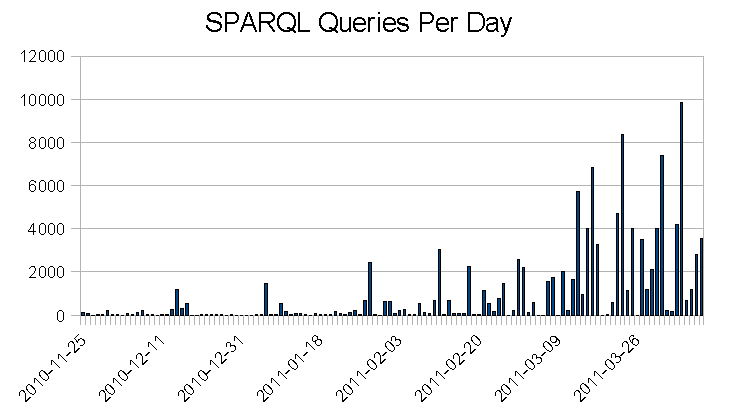
\includegraphics[width=0.5\textwidth]{images/SparqlQueriesPerDay.pdf}
%		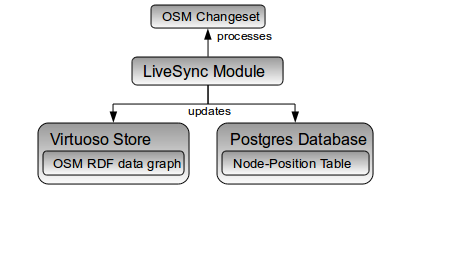
\includegraphics[width=0.4\textwidth]{images/LiveSyncArchitecture.png}
	\caption{Usage of the SPARQL endpoints.}
	\label{fig:sparql-queries-per-day}
\end{figure}
The diagram indicates that the LGD service is being actively used, and
that the usage rate is increasing.
%However, whether the high query counts towards the end remains at that level
%is yet to be evaluated.
%are one-shot or
%continuous uses need yet to be evaluated.

The current LGD release dataset contains about 65 million triples corresponding to
about 6.3 million nodes and 66 million triples corresponding to 7.1 million ways.
Table~\ref{tab:instance-counts} gives an overview of selected instance
counts in the static SPARQL endpoint, and their increase in number in LGD live
one after processing changsets corresponding to roughly three weeks.
\begin{table}[hb]
\begin{tabular}{lrr}
\toprule
class				&\#instances (static) & \#instances (live) \\
\midrule
Ways					&\val{7132373} &\val{7334925} \\
Nodes					&\val{6251067} &\val{7022481} \\
\midrule
Stream						&\val{2377952}	&\val{2419467} \\
Parking					&\val{520901} &\val{537477} \\
Village					&\val{516547} &\val{522570} \\
Shop					&\val{497820} &\val{519164} \\
Hamlet						&\val{415609} &\val{424179}\\
School				&\val{361239} &\val{366070} \\
PlaceOfWorship						&\val{359563} &\val{363225}\\
Restaurant &\val{173350} &\val{177888}\\
FastFood					&\val{67980} &\val{69772}\\
Pub 					&\val{67279} &\val{68279}\\
\bottomrule
\end{tabular}
\caption{Comparison of data from April 6th with live data from April 30th 2011.}
\label{tab:instance-counts}
\end{table}

Regarding LGD live sync performance, we measured the following values: on
average, the processing time of a single minutely OSM changeset takes 5 seconds with our filter configuration.
Between April 6 and April 30, about 40\,000 changesets were processed, each of them corresponding to an average addition of 620 and removal of 42 triples affecting 102 distinct resources.
%Evaluating 40K minutely changesets, each of them corresponds to
%an average addition of 620, and removal of 42 triples; affecting an average of
%102 distinct resources.

In the initial LGD release of 2009, there were 50 object properties.
However most of them were considered to be better suited as classes, resulting
in the relatively low number of only 9 object properties in the current
release.




%\begin{table}[htb]
%\renewcommand{\tabcolsep}{5pt}
%\begin{tabularx}{\textwidth}
%{
%>{\hsize=\hsize }L 
%>{\hsize=\hsize }L 
%>{\hsize=\hsize }L
%>{\hsize=\hsize }L 
%>{\hsize=\hsize }L 
%>{\hsize=\hsize }L 
%}
% \toprule
% \textbf{Interface}   &
% \textbf{Usage count} &
% \textbf{Avg. Time}   & 
% \textbf{P 1s}  & 
% \textbf{P 5s}  &
% \textbf{P 10s} & 
%\\
%\midrule
%Rest, Local-DB    &  5000 &   3   &    50\% &    50\% &    50\%  \\
%\midrule
%Rest, Osm-Wrapper &     - &   3   &    50\% &    50\% &    50\%  \\
%\midrule
%Sparql, Static    &  3000 &   3   &    50\% &    50\% &    50\%  \\
%\midrule
%Sparql, Live      &   100 &   3   &    50\% &    50\% &    50\%  \\
%\bottomrule
%\end{tabularx}
%\caption{Interface Performance Statistics}
%\label{tab:ips}
%\end{table}
%P-xs: What fraction of the queries could be answered within x seconds.
%Probably plot this as a graph, once we have that data.



\section{Tools using LinkedGeoData}
\label{sec:applications}

\begin{figure*}[tb]
	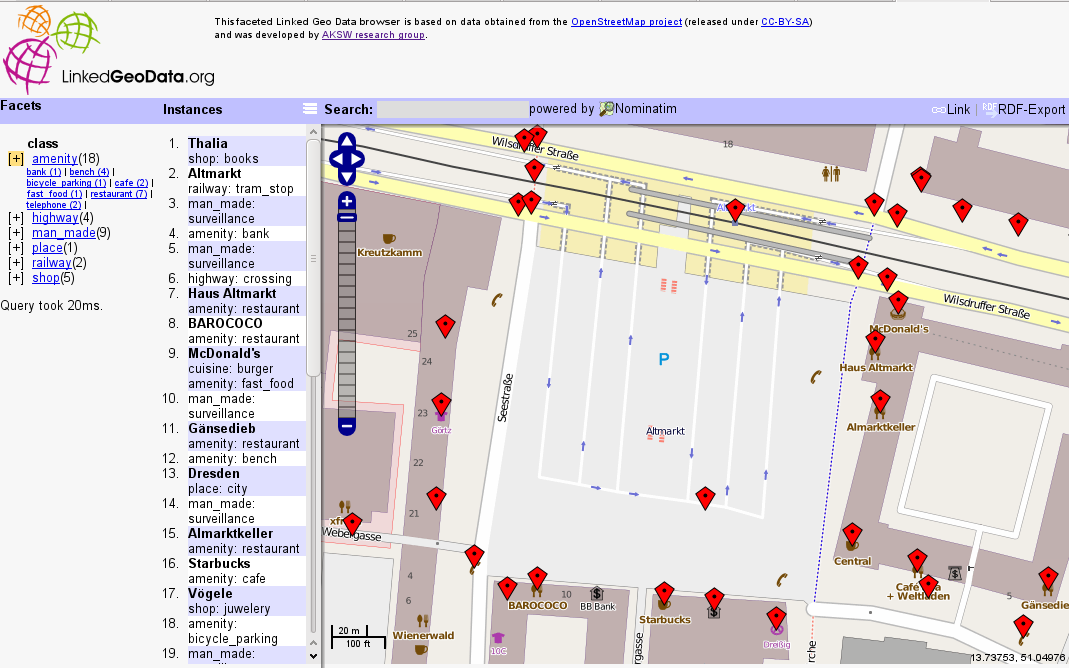
\includegraphics[width=.85\textwidth]{images/LGDBrowser}
	\caption{LinkedGeoData Browser.}
	\label{fig:browser}
\end{figure*}

\subsection{LGD Browser}
% JL: Browserbeschreibung ist teilweise aus dem ISWC-Paper uebernommen

In order to showcase the benefits of revealing the structured information in OSM,
we developed a facet-based browser and editor for
LinkedGeoData (see Figure~\ref{fig:browser})\footnote{Available online at: \url{http://browser.linkedgeodata.org}}.
It allows to browse the world by using a
``slippy map''\footnote{\url{http://wiki.openstreetmap.org/wiki/Slippy_Map}}.
Once a region is selected, the browser analyzes the descriptions of nodes and ways in that region and generates facets for filtering. Once a facet or a specific facet value has been
selected, matching elements are displayed as markers on the map and in a list.
If the selected region is changed, these are updated accordingly.

Performing the facet analysis naively, i.e. counting properties and property values
for a certain region, becomes slower the greater the size of 
the search region. This is due to the fact that the database has to
aggregate the facets from all the entities that fall into the search region.

To resolve this problem we precomputed tile-based statistics at various zoom
levels. If zoomed in close, the exact counts will be
measured, however if zoomed out the counts will be approximated by aggregating
the the statistics of the visible tiles.

Furthermore, there are several new smaller LGD browser features compared to its previous version described in~\cite{linkedgeodata}. For instance, an RDF export of the current map selection including its facets can now be performed.
This allows the easy extraction of a relevant fragment of LinkedGeoData for use
within other tools. For each point on the map, its RDF source can be retrieved and it can be edited on OpenStreetMap. The browser has been extended by a search function powered by \emph{OpenStreetMap Nominatum}. The facet support has been extended to object properties, i.e.~values of those properties can now be restricted in the facet selection. Finally, the LGD browser now provides a permanent link feature.

%Currently the tile ids are assigned according to the z-curve\todo{ref}
%numbering. This results in adjacent tiles having mostly a
%small difference between their ids. For this reason, lookups for tiles in an
%area This property results in which accounts for for efficient lookups


%Whether using 
 
%  tile ids are integers values that are assigned according to
% the
%z-curve\todo{ref} numbering. This results in adjacent tiles having mostly a
%small difference between their ids.  which accounts for for efficient lookups
%Whether using 

% can only use either the
%longitude or the latitude index. Combining both \-- longitude and latitude \--
%in one index is also impossible, since, given a certain latitude region, only
%elements in a relatively small longitude region are sought for.

%switch between two lookup strategies depending on the zoom level:
%When zoomed in close, the search region is small, and we perform the query
%query based on the nodes' positions. The postitions are indexed using 
%postgis' r-tree index.
%For each tile-id we then store the number of occurrences of the tags in it.
%When the user browses to a certain region, the application has to determine
%all the tiles intersecting that region.
%Since co-located tiles are assigned to adjacent tile ids, a certain region
%usually consists of a small number of tile ranges, which can be efficiently
%processed by the DBMS.


%\todo{Ok, This section drifted from reality, and now i broke it.}
%For computing the facets when zoomed out, we keep statistic tables that work
%as follows: At each zoom level, the map is divided into tiles, whereas the
%tiles are assigned ids according to the
%z-curve~\cite{zcurve}\footnote{Sometimes referred to as quadtile by the OSM
%community, see \url{http://wiki.openstreetmap.org/wiki/QuadTiles}} numbering.
%The consequence of the numbering is, that the ids of adjacent tiles are
%relatively close to each other, enabling efficient query evaluation with a
%B-Tree index. Note that   


%Even these indexing optimizations were not yet sufficient to obtain acceptable
%response times for the faceted browser. In order to further increase the
%querying performance, we precomputed the counts for all properties on all
%tiles, as well as the counts of all property values for a set of predefined
%properties of which we know that they have only a limited number of values.
%We did that not only for the highest zoom level, but for each zoom level which
%users are able to select. The lower the zoom level, the more the number of
%tiles reduces and the faster corresponding property and property value count
%aggregates can be computed.


\subsection{STEVIE}

STEVIE~\footnote{\url{http://tiny.cc/stevie10}}~\cite{stevie} is an application
developed by the Institute for Web Science and Technologies at the University of
Koblenz, which uses LinkedGeoData.
STEVIE allows one to create and edit points of interests (POIs)~(see
Figure~\ref{fig:stevie}) and annotate them semantically. The annotations use the LinkedGeoData ontology and are also interlinked to DBpedia. The annotations allow to employ clustering techniques in STEVIE, which are used to group sets of similar objects within the limited screen size of a mobile phone. The application allows the creation of events and, therefore, combines spatial and temporal information. An emphasis is put on providing an intuitive user interface for navigating those two dimensions. In order to display POIs and classify them, STEVIE uses the LinkedGeoData REST interface, ontology and SPARQL endpoint.

\begin{figure}[bt]
	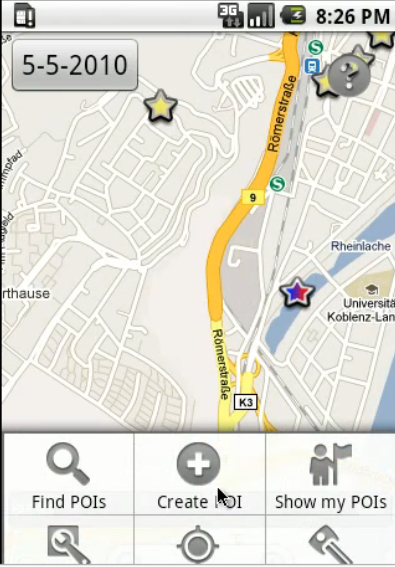
\includegraphics[width=.35\textwidth]{images/stevie}
	\caption{Creation of a point of interest in STEVIE. The application includes a temporal dimension and highlights POIs where events take place in the selected time span.}
	\label{fig:stevie}
\end{figure}

\subsection{BeAware}

BeAware\footnote{\url{http://beaware.at/}} is a website, which enables one
to manage events and integrates them with geographic information. It
uses its own ontology for events and integrates LinkedGeoData for choosing locations. In particular, the curated ontology of LinkedGeoData provides benefits for the application\footnote{\url{http://alexidsa-en.blogspot.com/2010/06/rdf-vs-nonrdf-for-geodata-at-beaware.html}}: ``First of all, LinkedGeoData ontology that connects all OpenStreetMap categories and properties excellently suits our interface of new place choosing (in addition, it allows to use inference engine, for example, for retrieving buildings of all types).'' Figure~\ref{fig:beaware} shows a screenshot for choosing the location of an event. An advantage gained by this association is that it facilitates querying for events at a particular location or within a particular city. In addition, in some cases further information about the location from an interlinked data source is available and can be presented to the user.

\begin{figure*}[htb]
	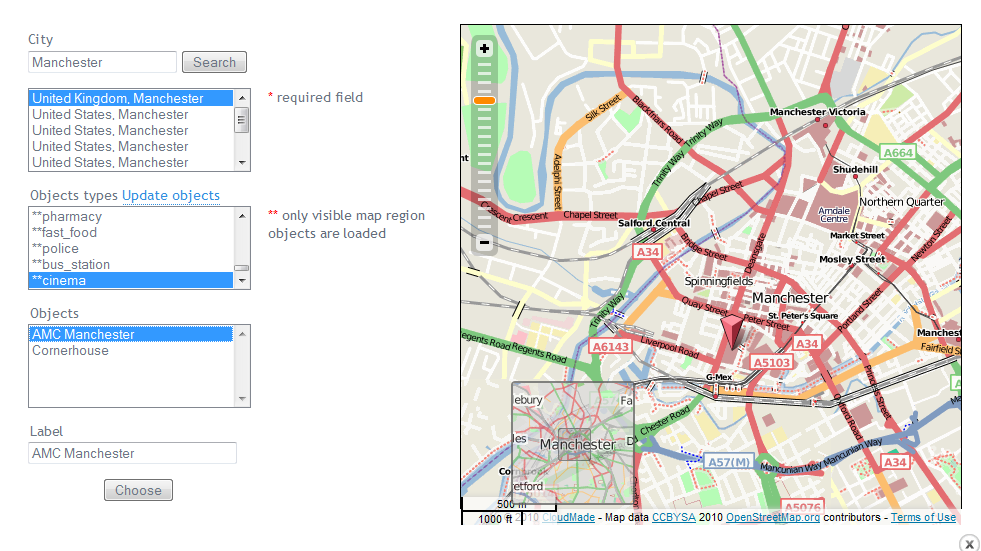
\includegraphics[width=.85\textwidth]{images/BeAware1}
	\caption{Marking the location of an event in BeAware.}
	\label{fig:beaware}
\end{figure*}

\subsection{Layar}

Layar\footnote{\url{http://www.layar.com}} is an augmented reality browser for mobile phones. Within Layar, a LinkedGeoData layer was developed. This allows to view the surrounding objects of a person via the mobile phone camera. The LinkedGeoData ontology is used to classify objects and map them to displayed icons. The layer uses \verb|rdfs:label|, which is aggregated from several tags in OpenStreetMap, to display the name of an object. Further triples describing an object are show in a detail view.

\begin{figure}
	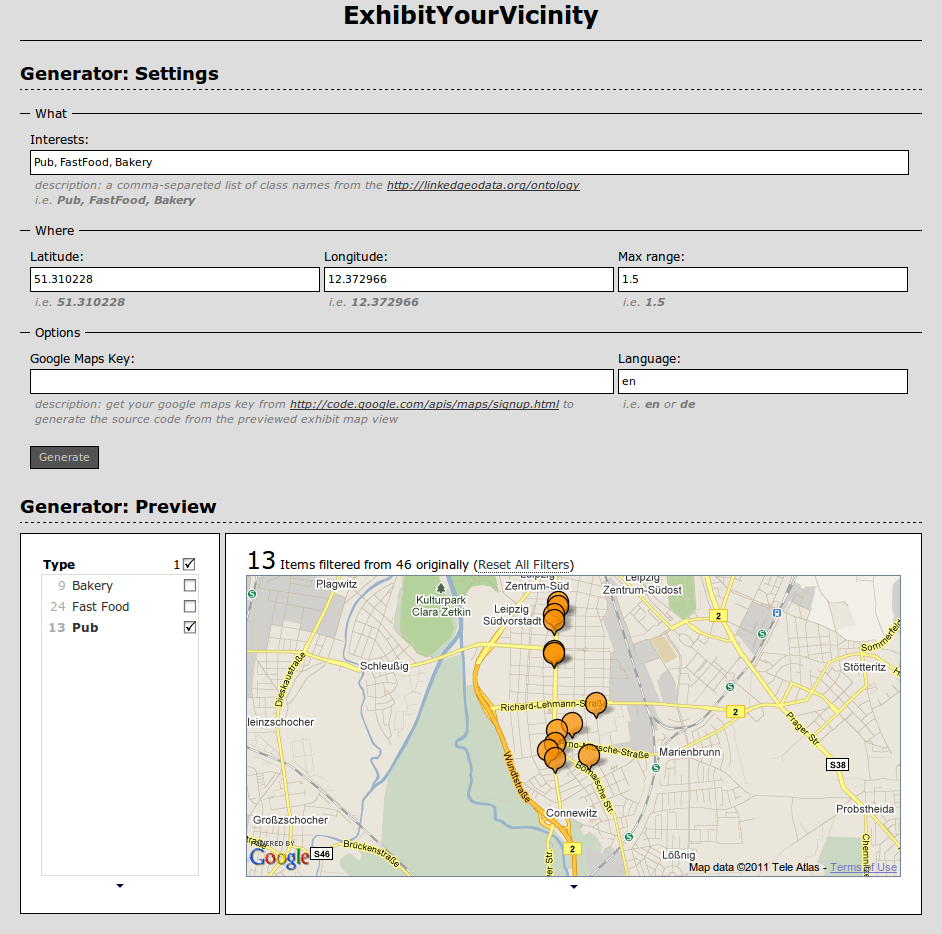
\includegraphics[width=.45\textwidth]{images/vicibit}
	\caption{Vicibit is a tool to generate custom views on LinkedGeoData via Exhibit. The example shows a faceted view on nearby pubs, bakeries and shops. The code generated by Vicibit can easy be pasted into blogs, forums and web pages.}
	\label{fig:vicibit}
\end{figure}

\subsection{Vicibit}

Vicibit\footnote{\url{http://vicibit.linkedgeodata.org}} (``exhibit your vicinity'') is a tool working on top of LinkedGeoData Live, which allows to create customised views on LinkedGeoData.
It enables users to pick classes from the LinkedGeoData ontology they are
interested in as well as a default map section, which should be displayed. The tool then generates HTML code, which creates a map displaying all items belonging to the selected classes as well as the ability to filter by facets. Technically, this is realised by applying the Exhibit framework\footnote{\url{http://www.simile-widgets.org/exhibit/}} on data in the LinkedGeoData Live SPARQL endpoint. A typical use case is that a webpage or blog entry describing a particular event can be enriched with a map of nearby pubs and other shops (see Figure~\ref{fig:vicibit}).



\section{Related Work}
\label{sec:related}

We split the presentation related work into five parts: 
First, we describe initiatives for integrating spatial information in the Web of Data. 
Afterwards, we summarize work on techniques for converting relational databases to RDF,
which is a crucial task we faced in LinkedGeoData. 
We then give an overview of triple stores supporting geographic data more complex than
point data. Finally, we review some related work done by the GIS community, give
pointers to interlinking frameworks and explain our choice of using SILK and LIMES.
 % and conclude with other related work, which we deem important, but does not fall into the three previous categories.

\subsection{Spatial RDF Datasets}

In the following, we describe spatial data sets, which are available as RDF and we consider important.

\begin{description}
\item \emph{Ordnance Survey}\footnote{\url{http://www.ordnancesurvey.co.uk}} is the national mapping agency in Great Britain. 
Over the past years, they released some of their products as Linked Data\footnote{\url{http://data.ordnancesurvey.co.uk}}. 
Ordnance Survey provides very accurate, high-quality data and represents a major contribution to the spatial data web. 
In a comparison between Ordnance Survey data~\cite{osm_ordnance_survey} focused on England and London in particular, OSM data was, however, also fairly accurate. 
A main difference between both efforts is that OpenStreetMap, and thereby also LinkedGeoData, are world-wide and community-driven approaches.
\item \emph{GeoNames} is a comprehensive global spatial database containing several million
features, such as cites, forests, and peaks.
This data has been converted to RDF\footnote{\url{http://www.geonames.org/ontology/}} and is served as Linked Data.
GeoNames provides RDF properties for navigating spatial hierarchies (parent/child), publishes postal codes, labels, population figures, type information (via feature codes) and other properties of spatial entities. 
Due to this wealth of information, we developed a fine-grained interlinking between LinkedGeoData and GeoNames as described in Section~\ref{sec:interlinking}. 
A difference between GeoNames and OpenStreetMap is that OSM allows free tags, which makes it easier to extend and tailor for new, previously unforeseen usage scenarios.
For instance, shops in OSM sometimes (specifically 60 thousand times as of April 2011) contain opening hours.
Another example is the wheelchair tag, used 24 thousand times, which indicates whether or not a spatial entity is accessible via a wheel chair. 
OpenStreetMap also has a larger community than GeoNames with several hundred thousand users and more fine-grained data, which even includes entities such as traffic lights or trash bins.
\item The \emph{United Nations FAO (Food and Agriculture Organisation) Geopolitical Data}~\cite{un_fao} provides RDF descriptions of countries and other political units as well as relations between them. 
While it contains only a small number of instances (298 in May 2011), it includes very detailed information on those instances. 
For this reason, we decided to provide interlinks with UN FAO.
% \todo{Jens: I looked at the data and in my opinion it would be easy and worthwhile to interlink it with LinkedGeoData countries (needs only a single SILK/LIMES spec.} => almost done
\item \emph{GeoLinkedData.es} is an open initiative to provide Spanish geospatial data~\cite{geolinkeddata}. 
It focuses on hydrography features and integrates several existing data sources.
\item \emph{NUTS (Nomenclature of Territorial Units for Statistics)} provides a hierarchical system for describing the economic territory of the European Union~\footnote{\url{http://epp.eurostat.ec.europa.eu/portal/page/portal/nuts_nomenclature/introduction}}. 
The NUTS hierarchy is established by EuroStat. EU NUTS data has been converted to RDF~\footnote{\url{http://rdfdata.eionet.europa.eu/ramon/nuts2008/}}. 
It allows to explore the hierarchy via Linked Data, e.g.~a possible path along the ``partOf'' property is  Inner London East $\to$ Inner London $\to$ London $\to$ UK.
\end{description}

\subsection{Relational Database to RDF Conversion and Mapping}

Converting relational databases to RDF is a significant area of research with several approaches published and many tools available. 
In particular, there is the W3C RDB2RDF working group, which aims to standardize a database to RDF mapping language~\cite{r2rml}. 
Instead of providing an in-depth overview, we refer to recent surveys~\cite{RDB2RDF,SWJ_RDB2RDF}  and overviews\footnote{\url{http://esw.w3.org/topic/Rdb2RdfXG/StateOfTheArt}} on this topic.
%\url{http://esw.w3.org/topic/Rdb2RdfXG/StateOfTheArt}
%\url{http://www.w3.org/2005/Incubator/rdb2rdf/RDB2RDF_SurveyReport.pdf}
%\url{http://www.semantic-web-journal.net/content/bringing-relational-databases-semantic-web-survey}
There are various tools available implementing the surveyed approaches such as D2R, Triplify, DartGrid, DataMaster, MapOnto, METAmorphoses, ODEMapster, RDBToOnto, RDOTE, Virtuoso RDF Views and VisAVis. 
For LinkedGeoData, we decided to use a custom mapping solution as described in Section~\ref{sec:rdf_mapping}, despite the number of available conversion tools. 
The reason for this choice was the particular tag structure of OSM, which allows us to provide a highly flexible schema as well as handle a very high amount of data via our approach.
% This way, a live synchronisation with OpenStreetMap is feasible.


%reviewt drei Gezetteere (GeoNames, Getty, und ADL)
%  und diskutiert design entscheidungen und implementation einer OWL
%  Ontologie, wie sie auch für similarity searches verwendbar ist.

%Implementations of 
% gibt eine ausführliche diskussion über such
%paradigmen (intensional, extensional, hybrid) in bezug auf von SIM-DL, eine
%similarity theorie für beschreibungslogiken, und diskutiert eine architektur,
%um SIM-DL in SDI (spatial data infrastructure) zu integrieren.

% (Spatially-Aware Information Retrieval on the
% Internet) SPIRIT\cite{intelligent_spatial_search} ist eine (wenn nicht
% velleicht damals die) weitere spatially aware suchmaschine.
  
%research topics bei solchen such engines sind:
%grounding (lokalisierung), disambiguierung, query expansion (z.B. semantisches
%anreichern von queries), ranking, fuzzy spatial relations (``near'')
  
  
\subsection{Triple Stores supporting Complex Geometries}
\label{sec:geo-semantic-web}

In the relational database realm, support for complex geometric data
(points, lines, and polygons) is already well established. Examples are
MySQL\footnote{\url{http://www.mysql.com}},
PostgreSQL\footnote{\url{http://www.postgresql.org/}}, and
Oracle\footnote{\url{http://www.oracle.com}}.
Meanwhile, in the Semantic Web, the support for geometric data has also
increased significantly. Currently, we are aware of four triple stores
supporting this kind of data:
\emph{OWLIM Standard Edition}\footnote{\url{http://www.ontotext.com/owlim/geo-spatial}}
(OWLIM-SE, previously known as BigOWLIM),
\emph{Open Sahara}\footnote{\url{http://opensahara.com}},
\emph{Parliament}\footnote{\url{http://parliament.semwebcentral.org/}}, and
\emph{AllegroGraph}\footnote{\url{http://www.franz.com/agraph/allegrograph/}}. 

So far there has not been a standard query language for geospatial
data in the Semantic Web. GeoSPARQL is a proposed extension to
SPARQL~{1.0}~\cite{sparql} with the aim to provide this functionality.
It is currently at the stage of becoming a standard by the Open Geospatial consortium\footnote{\url{http://www.opengeospatial.org/}}.   
With these tools, tasks that require complex operations on geometries
become possible in the Semantic Web.
%  This effort can be expected to eventually become supported by RDB-RDF mapping solutions.
% \todo{ideally add the post office
%use case if I ever find this paper again (Something along the lines of Peter
%met Sarah across the street at the post office. System plots likelyhood of
%where they met.)}
  
We chose Virtuoso as the backend for LinkedGeoData because of its good
performance~\cite{BerlinSparql} and our assumption that point geometries
would be sufficient for most of our interlinking tasks. Although this turned
out to be true, in the future we want to extend these tasks to complex
geometries and therefore also evaluate the other stores.

\subsection{Gazetteer Mapping}

Our interlinking approach is very similar to the matching of gazetteers in
traditional Geographic Information Systems (GIS): \cite{gazetteer_core_elements}
discusses the alignment of two major gazetteers. For this
purpose, place names, types and footprints (geographical entities such as
point, lines and polygons) were identified as the most fundamental features of gazetteers.
These entities closely resemble the concepts of classes, labels and
geometries, on which we based our interlinking.
Prior work about the derivation of an OWL ontology suitable for similarity
searches from gazetteers is given in \cite{gazetteer_ontology}. 
A comprehensive discussion about similarity search paradigms
for Description Logics is lead in \cite{sim_ir}.

\subsection{Interlinking and Ontology Mapping}

There have been several decades of research starting with the integration of
different database schemata. Tools like COMA~\cite{coma} provide rich support
for various matching operations between databases as well as between RDF
knowledge bases. \cite{BraunerIFC07}~describes a semantic approach for matching
export schemas of geographical database Web services, based on the use of a
small set of typical instances. The paper also contains an extensive
experiment, carried out within the context of two gazetteers, GeoNames and the
ADL gazetteer, to illustrate the idea. \cite{conf/icdim/ManguinhasMB08}
describes an approach integrating spatial data from multiple sources, which also
incorporates a temporal dimension. For interlinking LinkedGeoData, we mainly
searched for instance matching tools, since our main goal is to match specific
points of interests in different knowledge bases. In this area,
SILK and LIMES are the most widely used applications. We extended
SILK with an appropriate metric for matchings based on WGS84 distance between
points, which was later included in the official SILK release. A main benefit
for SILK as well as LIMES, which we both use, is their ability to handle large
volumes of data and use SPARQL endpoints as input source.

\begin{comment}
\url{http://de.wikipedia.org/wiki/Web\_Map\_Service}
\url{http://de.wikipedia.org/wiki/Web\_Feature\_Service}

Analysis of edit behaviour:
"Annotating Spatial Features in OpenStreetMap"

Current work in the area of spatio temporal data can be roughly classified
into RDF-Conversion, Interlinking, RDB-RDF mapping and ontology engineering,
(whats more?) \todo{what else}.

Workshop On Linked Spatiotemporal Data 2010
   \url{http://stko.psu.edu/lstd2010/}

Thing the people from the NeoGeoVocabCamp are working on
    GeoLinkedData
g2r
d2g

Das ist das tolle Dokument:
\url{http://linkeddata.com.ar/doc/2011/03/note.html}
\end{comment}

\section{Conclusions and Future Work}
\label{sec:conclusions}

The transformation and publication of the OpenStreetMap data according to the
Linked Data principles adds a new dimension to the Data Web: spatial data can
be retrieved and interlinked on an unprecedented level of granularity. These
enhancements may further contribute to semantic-spatial search engines, such as
~\cite{sim_ir, spirit}, and enable a variety of new Linked Data applications such
as geo-data syndication (publishing information about geographical entities via
feeds). Another example is personalized and context-sensitive
spatial Linked Data update propagation and consumption, which might be
realized with systems such as sparqlPuSH~\cite{sparql_push}.
 

The dynamics of the OpenStreetMap project will
ensure a steady growth of the LinkedGeoData dataset. Furthermore, we established mappings with DBpedia and GeoNames as the central interlinking hubs for spatial information on the Web of Data.
Despite the recent advances in RDF data management, it became clear during our work on LinkedGeoData that spatial data of the size of OpenStreetMap still poses a major challenge wrt. scalability.
Substantial engineering effort was required to optimize the performance of the querying interfaces, live synchronisation as well as the interlinking.

Currently, our transformation approach imposes the following\emph{ limitations} on the use of
LinkedGeoData:
\begin{itemize}
  \item The current \emph{ontology} is mainly automatically derived from
  OpenStreetMap tags, with mostly just minor manual edits. However, it could
  benefit from axiomatizations, such that, for example, any \emph{PlaceOfWorship} with religion
  \emph{christian} is a \emph{Church}.
  The extent to which the addition of disjointness axioms makes sense needs yet
  to be investigated. For instance, currently instances corresponding to
  hotels that also offer a restaurant are currently tagged with both types.
  However, an alternative solution would be to model such instance as a
  \emph{Hotel}, that offers a feature that is a \emph{Restaurant}. For these
  kinds of design decisions, we envision a solution similar to the \emph{DBpedia
  Mapping Wiki}\footnote{\url{http://mappings.dbpedia.org}}, that enables the
  community to contribute to the axiomatization of the ontology.
  
  \item Our \emph{filtering} (see Section~\ref{sec:filtering}) currently
  discards a significant amount of data from OSM. Hence, there are use
  cases that are possible with OSM data, but not with LinkedGeoData yet.
  For example, since we filter out ways with more than 20 nodes, 
  routing\footnote{\url{http://wiki.openstreetmap.org/wiki/Routing}} is currently not
  possible based on the LinkedGeoData SPARQL endpoints.
    
  \item Because we do not support OpenStreetMap relations yet, information about
  compound entities is also not yet available in LinkedGeoData. 
  Examples of such entities are: multipolygons (collections
  of polygons, where each member may act either as solid or as a hole), or
  designation signs. Further examples include large boundaries, waterways, and
  routes, that are modelled with way segments.
\end{itemize}

As for the latter two limitations, we are currently investigating whether and
how these limitations can be overcome by directly rewriting SPARQL queries to SQL queries over
the relational schema of OpenStreetMap.
Although substantial progress was made in RDB-RDF mapping
during the last years, and implementations are now more robust, scalability
and the lack of support for geometry datatypes is still an issue
preventing a direct deployment of these technologies for LinkedGeoData.

Another stream of future work is the better support for geometries according to
the current NeoGeoVocabulary
development\footnote{\url{http://geovocab.org/doc/neogeo.html}}, which we are
supporting. A semantic misrepresentation currently found in LinkedGeoData, for
example, is the missing separation of geometries (such as points and polygons)
and features (such as hotels and pubs), which we plan to resolve in the future.
%In the future, we plan to implement thi
%plan to attach geometries to entities, i.e. points of interest, instead of
%identifying both.

Finally, we identified further candidates that seem worthwhile for interlinking:
\begin{itemize}
\item The \emph{CIA World
Factbook}\footnote{\url{https://www.cia.gov/library/publications/the-world-factbook/}}
contains detailed information on the country level, such as their conventional
names, their birthrate, and their gross domestic product. An RDF version is
hosted by the Free University of
Berlin\footnote{\url{http://www4.wiwiss.fu-berlin.de/factbook/}}.

\item The site \url{climb.dataincubator.org} hosts a collection of data of about
{1400} climbing locations with latitude/longitude information. The resources
were collected from various climbing web sites and converted to RDF.

\item \emph{Last.fm}\footnote{\url{http://last.fm}} has information about music
artists, as well as events, such as performances and festivals. Many event locations are
geo-tagged, making them suitable candidates for interlinking.
There exist at least two wrappers for the {last.fm} API that return
RDF\footnote{\url{dbtune.org/last-fm/} and \url{lastfm.rdfize.com/}}.

\end{itemize}



%\section*{Acknowledgments}
%We would like to thank OpenLink for providing an enterprise
%edition of the Virtuoso database system that offers support for spatial SPARQL
%queries. Furthermore, the authors thank the members of the LinkedGeoData
%community and 3rd party application developers for their valuable feedback and contributions to the project.
%In particular, we would like to mention Robert Schulze for his work on Vicibit.
%This work was supported by a grant from the European Union's 7th Framework
%Programme provided for the projects LOD2 (GA no. 257943) and LATC (GA no. 256975).

%%%%%%%%%%% The bibliography starts:
%\bibliographystyle{abbrv}
%\bibliography{swj_linkedgeodata,../../bib/aksw}

%\appendix

\section{Prefixes Used}
\label{sec:prefixes}

The following prefixes are used in the paper:

\begin{ttfamily}
\begin{lstlisting}[language=SQL,basicstyle=\scriptsize,numbers=left,numberstyle=\tiny,breaklines=true,breakindent=0cm,breakautoindent=false,morekeywords={OPTIONAL,FILTER}]
lgd:    http://linkedgeodata.org/triplify/
lgdo:    http://linkedgeodata.org/ontology/
wgs84:   http://www.w3.org/2003/01/geo/wgs84_pos#
foa:     http://www.fao.org/countryprofiles/geoinfo/geopolitical/resource/
dbpedia:  http://dbpedia.org/resource/
rdf:      http://www.w3.org/1999/02/22-rdf-syntax-ns#
rdfs:     http://www.w3.org/2000/01/rdf-schema#
owl:      http://www.w3.org/2002/07/owl#
xsd:      http://www.w3.org/2001/XMLSchema#
georss:   http://www.georss.org/georss/
\end{lstlisting}
\end{ttfamily}

%\end{document}



% Analytics


\section{Introduction}
Query logs allow us to bridge the theory and practice of SPARQL ~\cite{MartensT19}. These query logs ensure that the research conducted by the community is guided by the requirements and trends that emerge in practice.
The real-world SPARQL queries that are collected from public SPARQL endpoints have multiple use-cases such as performance evaluation in real-world settings, improve caching of triplestores, analysis on SPARQL adoption, query optimization, and usability analysis etc. \cite{stadleralsq}. The query logs produced by different SPARQL endpoints use different formats to syntactically represent records. In this work we consider Web Log Format and CSV. Within each format, the set of available fields -- the schemas -- vary. For example, the formats used by wikidata, bio2rdf, and virtuoso instances in default configuration are different schema variants of the Web Log Format~\cite{stadleralsq, SaleemAHMN15}.
%JSON etc
%In addition, these query logs often have formatting issues, making it difficult for a parser to extract required information from these logs. 
Furthermore, in order to utilize real-world SPARQL queries in the aforementioned use-cases, it is required to parse these queries and annotate them with various structural and data-driven features such number of triple patterns, list of projection variables used, the different types of joins used, the results size etc. Finally, annotating SPARQL queries in existing query logs needs a scalable processing engine. For example, DBpedia public SPARQL endpoint receives more than 100k queries everyday. Similarly, the Wikidata public endpoint receives thousands of queries on daily bases. 

To the best of our knowledge, there exist no generic and scalable software framework that parses these query logs to extract SPARQL queries, annotate them with different information, and convert them into an RDF dataset. 
To fill this research gap, we present the LSQ framework, which converts
SPARQL query logs into RDF dataset and attach various structural and data-driven features to each SPARQL query. In order to perform scalable RDF conversion, we make use of the Apache Spark Big Data framework. By default, the framework supports query logs from nine different formats. Support for other logs formats can be easily done by adding log patterns into the configuration file.  

This framework has already been used to convert query
logs of 27 public SPARQL endpoints from various public SPARQL endpoints such as DBpedia, Wikidata, Bio2RDF, Semantic Web Dog Food etc. The resulting RDF datasets are named as LSQ V2.0 \cite{stadleralsq}. The LSQ V2.0 represents 43.95 million executions of 11.56 million unique SPARQL queries, resulting in 1.24 billion triples.  
The LSQ queries have been used in many use cases such as benchmarking based on real-world SPARQL queries \cite{SaleemMN15,SaleemMSLN18,saleem2018largerdfbench,SaleemSCBMN19,hernandez2016querying,fernandez2019evaluating,azzam2020smart,bigerl2020tentris,AzzamAMKPH21,davoudian2021workload,9364498,9364380}, analysis of the SPARQL adoption in different applications \cite{han2016statistical,BonifatiMT17,bonifati2018darql}, improving caching strategies for SPARQL engines \cite{knuth2016scheduling,akhtar2018change,akhtar2019dynamic,SalasH18,safavi2019personalized}, useability analysis of the SPARQL \cite{arenas2016reverse,benedetti2016model,dellal2017addressing,stegemann2017investigating,Viswanathan18,Potoniec19,wang2019answering,BonifatiMT20,jian2020sparql,zhang2020revealing,ALMENDROSJIMENEZ2021113772,wang2021explaining}, and SPARQL query optimization \cite{song2016efficient,MartensT18,cheng2019opt+,FigueiraGKMNT20}. Since the initial release of the LSQ V1.0 \cite{SaleemAHMN15}, the datasets converted by our framework have been used in more than 50 research papers\cite{stadleralsq}. The scalable components developed into the LSQ framework have also contributed to the recent Apache Jena 4.6.0 release with additional improvements pending\footnote{For details please see: https://github.com/apache/jena/pull/712, 
https://github.com/apache/jena/pull/1475,
https://github.com/apache/jena/pull/1394, 
https://github.com/apache/jena/pull/1390, 
https://github.com/apache/jena/issues/1470, https://issues.apache.org/jira/projects/JENA/issues/JENA-2309}. 

The rest of the paper is organized as follows. In section 2, we present the LSQ framework. Section 3 discusses various use-cases where the datasets produced by our framework have already been used. In section 4, we present the useability instruction of this framework, followed by the availability information and sustainability plans in section 5. Finally, we conclude in section 6. 

\section{The LSQ Framework}
\begin{figure*}
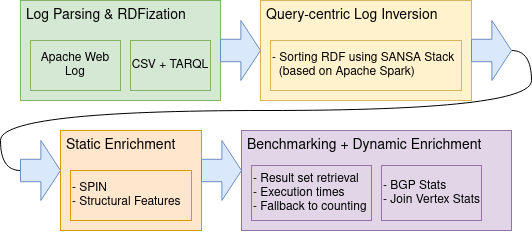
\includegraphics[width=\textwidth]{images/lsq2-architecture-new}
\caption{LSQ Framework Architecture. The underlying Semantic Web framework is Apache Jena.}
\label{fig:architecture}
\end{figure*}
In this section, we first briefly explain the core architecture. The details of each component is explained later. 

\Cref{fig:architecture} shows the architecture of LSQ which is briefly summarized as follows.
Records of query logs in different formats and having different schemas are parsed and normalized as RDF. 
The RDF log is inverted such that every query is related to all log records that mention it, i.e., every query is assigned a global (w.r.t, all query logs from different endpoints) identifier. 
In this process, queries are represented by hashes computed with their normalized strings. Static enrichment basically extracts the static features (that can be directly derived from a SPARQL query without running it against a specific RDF dataset) relevant to SPARQL query. It extends the RDF model with a SPIN\footnote{SPARQL SPIN representation: \url{https://www.w3.org/Submission/spin-sparql/}} and further static structural features such as the number of projection variables, number of triple patterns, join types and selectivities, the used syntactic elements (e.g. UNION, OPTIONAL) etc. %Furthermore, LSQ captures information about basic graph patterns (BGPs) which do not have a direct representation in the SPIN model. 
The dynamic enrichment extracts data-driven SPARQL features such as query runtime, result size or triple pattern selectivities etc.  Whereas static enrichment is independent on any dataset, dynamic enrichment needs a dataset as input. Benchmarking is a form of dynamic enrichment that extends a query's RDF model w.r.t. a dataset with result set sizes and execution times.
In the following, we present these steps in detail and how
%LSQ conceptual contributions as well as how
LSQ inspired creation of certain components which we contributed to other frameworks in order to facilitate reuse.
% something like: and how lsq makes conceptual contributions and how contributions to other frameworks were inspired by lsq



\subsection{Named Graph Stream Processing}
A fundamental design principle that is followed throughout LSQ is the \emph{entity graph} paradigm, also referred to as (named-)graph-per-entity:
An entity is represented by an IRI that appears in a (subject position of) triple in a named graph with the same IRI, such as \texttt{GRAPH :anEntity \{ :anEntity :p :o \}}.
Some Semantic Web tools (such as Virtuoso and Apache Jena) already support the use of named graphs with \texttt{CONSTRUCT} queries due to popular demand\footnote{\url{https://github.com/w3c/sparql-12/issues/31}}, although this feature is not part of the current SPARQL specification v1.1\footnote{\url{https://www.w3.org/TR/sparql11-query/}}.
LSQ uses the entity graph approach for representing log records and SPARQL queries.
The advantage of this approach are:
\begin{itemize}
\item The graph name acts as a natural entry point for starting exploration/traversals of the contained data. This is a convention applications (such as viewers) can support without having to rely on a specific (ad-hoc) vocabulary.
\item Retrieval and removal of all triples related to an entity is a simple operation on the named graph. This is of particular importance as certain models (e.g. SPIN) allow for arbitrary deeply nested tree structures in RDF which are extremely hard to query without scoping by a named graph.
\item Partitioning the data into self-contained named graphs is well aligned with the map-reduce paradigm: Operations on individual entities, such as enrichment operations, can be carried out naturally in parallel over a set of entity graphs using conventional Big Data frameworks. We created the necessary hadoop-based parsers as part of LSQ and contributed them to the SANSA stack (see \Cref{sec:sansa}).
\item An operation on an individual entity typically only requires its graph to be loaded rather than requiring access to \emph{all} triples across all entities, which allows for stream-processing with low memory usage.
\end{itemize}


% design issue that needed resolution was how to represent the information extracted from SPARQL queries.
%Initially, each logged query was directly transformed to RDF triples. However, this made it impossible to later extract retrieve all triples related to a specific
%query: The RDF model\todo{figure} of a query contains data along quite long paths. Furthermore, the spin model can represent arbitrarily nested RDF graphs.
%For this reason, the design choice was to use a \emph{graph-per-entity} approach 

\subsection{Parsing Query Logs}
Generally, LSQ parses query logs and transforms them into a set of named graphs of which each represents an individual log record. This means that every log file is harmonized to a common RDF model.

Query logs come in different formats, and within a format there can be many different schemas. By schema we refer to the set of available attributes per log record.
Manually determining the format and schema of a log is a very tedious task.
For this reason, LSQ features a log format registry which can be used to probe log files against.
Currently 2 types of log formats are supported: Web access log formats that are compatible with Apache HTTP server's mod\_log\_config\footnote{\url{https://httpd.apache.org/docs/current/mod/mod_log_config.html}}
and CSV. For the former, LSQ provides a custom mapping of log fields to an RDF model, for the latter a tarql-based\footnote{\url{https://github.com/tarql/tarql}} approach is supported where columns of the input file are mapped to RDF using a SPARQL construct query. Support for additional mapping languages, such as RML~\cite{dimou2014rml} or YARRML~\cite{Heyvaert2018Declarative} is future work. Note, that for the task of RDFizing a single CSV file, the practical difference between the approaches lies in syntax rather than functionality.

An excerpt of LSQ's log format registry configuration is shown in \Cref{lst:log-fmt-registry}.
So far the default registry comprises 10 formats/schema combinations.


\begin{lstlisting}[label=lst:log-fmt-registry, caption=RDF-based log format registry used in LSQ, style=lst, language=ttl, float=*, numbers=left]
fmt:combined
  a lsq:WebAccessLogFormat ;
  lsq:pattern "%h %l %u %t \"%r\" %>s %b \"%{Referer}i\" \"%{User-agent}i\"" .

fmt:bio2rdfProcessedCsv
  a lsq:CsvLogFormat ;
  lsq:pattern
"""
PREFIX lsq: <http://lsq.aksw.org/vocab#>
PREFIX prov: <http://www.w3.org/ns/prov#>
PREFIX xsd: <http://www.w3.org/2001/XMLSchema#>
CONSTRUCT {
  GRAPH ?s {
    ?s
      lsq:query ?query ;
      lsq:host ?domain ;
      lsq:headers [ <http://example.org/header#User-agent> ?agent ] ;
      prov:atTime ?t
  }
} {
  BIND(IRI(CONCAT('urn:lsq:', MD5(CONCAT(?query, '-', ?domain, '-', ?timestamp)))) AS ?s)
  BIND(STRDT(?timestamp, xsd:dateTime) AS ?t)
}
""" .
\end{lstlisting}



\subsection{Accessing RDF graphs via Object Models}

\begin{figure*}
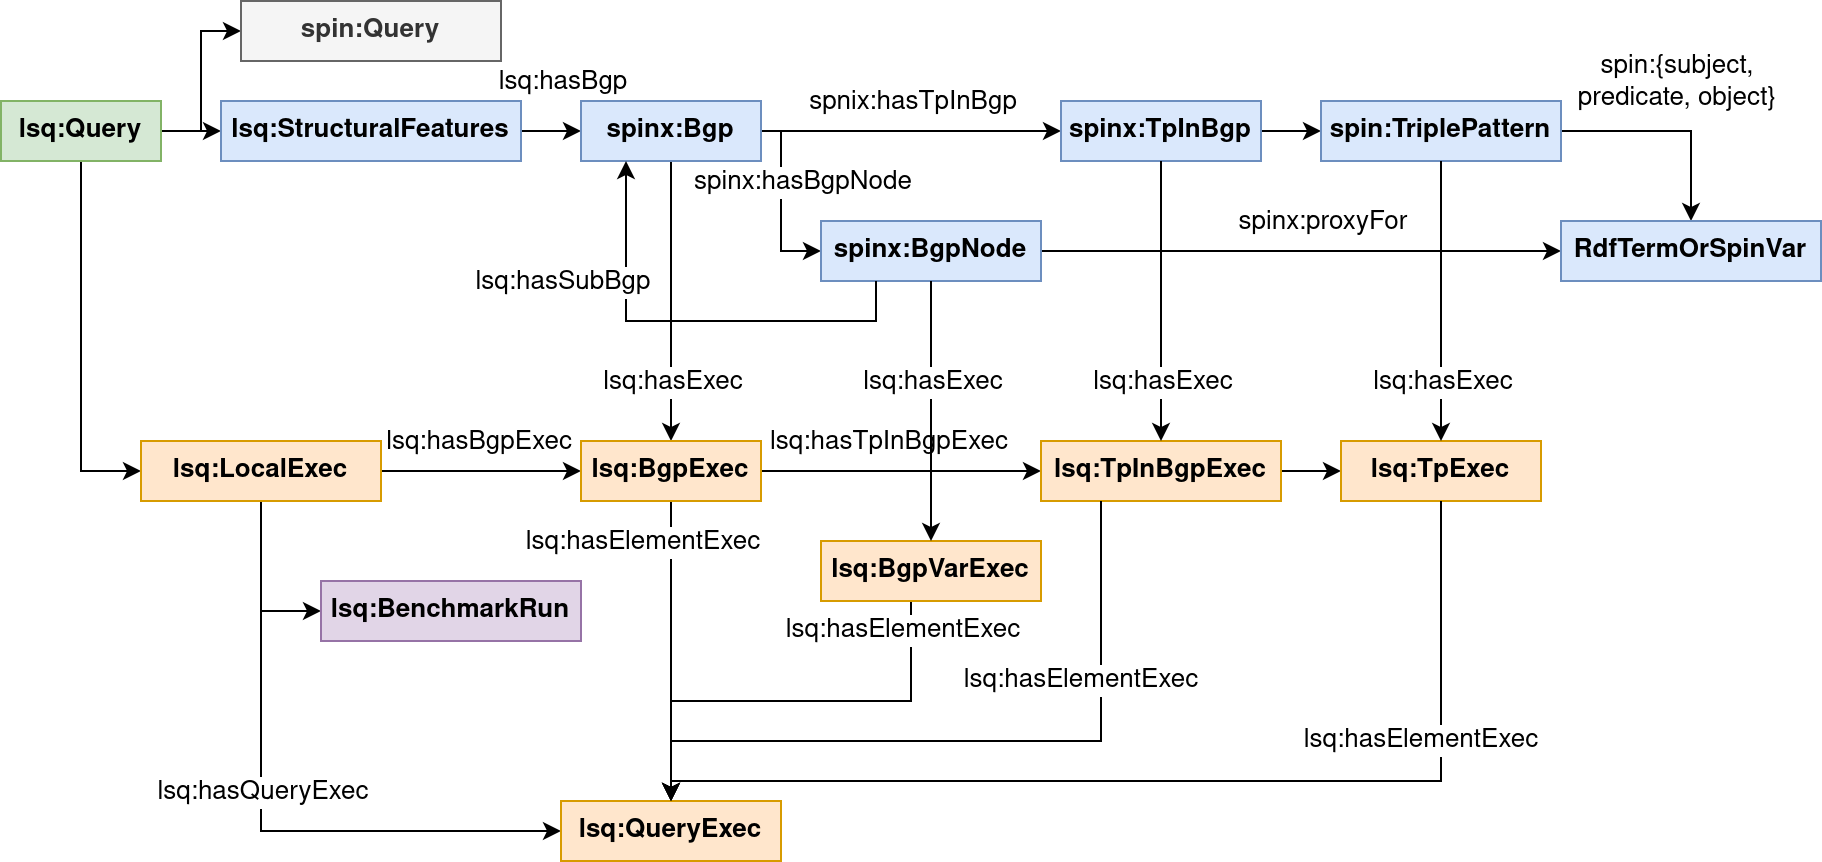
\includegraphics[width=\textwidth]{images/lsq2-datamodel-color-large}
\caption{LSQ2 Data Model}
\label{fig:datamodel}
\end{figure*}

The LSQ data model (see \Cref{fig:datamodel}) is sufficiently complex such that manipulation solely
with SPARQL turned out to be infeasible. One of the main reasons is due to the redundancy of complex graph patterns: Many patterns have to be repeated over and over again in different queries in order to address the nested resources. %which enrich.
Especially during development, any change in the T-box requires a change in several places and debugging SPARQL queries that yield empty result sets is a tedious process. Furthermore, deterministic skolemization of the model is an important aspect: We strictly want to avoid effects such as a merge of a query's RDF resulting in doubling the number of related BGPs as would be the case if blank nodes were used. Therefore, we need a way to express how to compute the identity of entities, such as: the id of a triple pattern depends on the id of its subject, predicate and object components, the id of a BGP depends on the ids of the contained triple patterns (in order) and the id of a specific triple pattern in a BGP depends on that of the BGP and its own.
%in order to avoid incorrectly repeating information such as the set of BGPs that are present in the model.

For this purpose, LSQ features a domain model realized as Java interfaces which must extend from Jena's \texttt{Resource} interface. The essence is, that the auto-generated implementations for this domain model then provides a \emph{view} over the RDF graph; all state is kept in the RDF graph and any invocation of a ``setter'' method directly mutates the RDF graph whereas a ``getter'' method reads from it.
Annotations on these interfaces are used to describe how getters and setters relate to triples in the underlying RDF graph. We use \emph{Reprogen} (Resource Proxy Generator)\footnote{\url{https://github.com/Scaseco/jenax/tree/develop/jenax-reprogen-parent/jenax-reprogen-core}} to generate Java proxies that implement the intended behavior of the annotations.

In order to realize skolemization, we extended Reprogen with new \texttt{@HashId} and \texttt{@StringId} annotations.
@HashIds are a way to control how to compute hash codes for an RDF term in an RDF graph w.r.t. to the annotated interface.
%If a method whose return value is neither a blank node nor IRI is annotated with @HashId then that value corresponds to a node at the boundary of a CBD. Hashes are computed for these literal values directly.
The hash code of a resource is obtained by recursively considering the hash codes of all its member methods annotated with \texttt{@HashId}.
The \texttt{@StringId} annotation is used for methods that can convert hash codes to strings suitable for use in IRIs.
%\Cref{lst:reprogen} shows an example for how to annotate a class whereas~\Cref{lst:reprogen-skolem} shows how to programmatically generate the corresponding RDF.
\Cref{lst:reprogen-skolem} shows how to programmatically generate RDF for an annotated class whereas
\Cref{lst:reprogen} shows an example for how to annotate a class.

%Otherwise, the HashId computation traverses along IRIs or blank nodes until non-resource attributes are encountered. %Hashes are the computed by performing a depth-first traversal to the boundary of the CDB,

\begin{lstlisting}[label=lst:reprogen-skolem, language=java, caption=Example for setting up and skolemizing a basic LSQ RDF model, style=lst, language=java, numbers=left]
Model model = ModelFactory.createModel();
LsqTriplePattern tp = model.createResource(LsqTriplePattern.class);
TpInBgp tpInBgp = model.createResource(TpInBgp.class);
tp.setJenaTriple(new Triple());

Resource root = Reprogen.skolemize(tpInBgp, "http://lsq.aksw.org");
RDFDataMgr.write(System.out, root.getModel(), RDFFormat.TURTLE_PRETTY);
\end{lstlisting}


\begin{lstlisting}[label=lst:reprogen, language=java, caption=Example of LSQ's annotated Java domain model for which Reprogen generates proxy implementations that can read and write to an RDF graph, style=lst, language=java, float=*, numbers=left]
/* The identity of a bgp depends on the list of identities of the contained
 * triple patterns */
public interface Bgp
 extends Resource
{
  @HashId
  @Iri(LsqTerms.hasTp)
  List<LsqTriplePattern> getTriplePatterns();
}

/* The identity of a "triple pattern in a bgp" depedends on the identity of
 * the bgp and the identity of the triple pattern */
public interface TpInBgp
  extends Resource
{
    @HashId
    @Iri(LsqTerms.hasBgp)
    SpinBgp getBgp();
    TpInBgp setBgp(Resource bgp);

    @HashId
    @Iri(LsqTerms.hasTp)
    LsqTriplePattern getTriplePattern();
    TpInBgp setTriplePattern(Resource tp);
}

\end{lstlisting}


%Maintaining skolemization in SPARQL queries using e.g. \texttt{BIND(IRI(CONCAT(STR(?baseIri), %'/aspect) AS ?aspect)} became infeasible.
%The requirements are as follows:
%\begin{itemize}
%\item A means to navigate a query's RDF model from LSQ's host language (Java).
%\item A mechanism to annotate which properties of a resource contribute to that resource's %identity.
%\end{itemize}


\subsection{Query Id Generation}
An important requirement in LSQ is determinism: Syntactically equivalent queries and their elements should always be represented by the same IRIs. The goal is to allow for the integration of different datasets generated by the same version of LSQ simply by means of merging the RDF.
Generally, query strings are normalized using a parse/string serialization round trip.
Query strings themselves are not suitable as identifiers because they can become very lengthy.
The obvious choice is thus to resort to hashing. LSQ v1 used 8 characters of md5 hashes however it turned out that the number of queries was sufficiently large that collisions occurred.
LSQ v2.0 uses sha256 with base64 encoding of the whole query string. The disadvantage was,
that queries that only differed in projection or slice received unrelated hashes. As a consequence, identifying queries that only differ in their 'basic parameterization' was not possible from the hashes.
LSQ v2.1 introduces additional structure:
The \emph{body hash} of a query is obtained by replacing the projection with 'SELECT *' and applying sha256+base64 hashing on the normalized query string.
A separate hash is computed from the projection: 
The actual projection expression strings are first sorted lexicographically and a projection-base-hash is computed from these ordered strings. The actual projection is then permutation of the sorted one, and numbering schemes exist to label permutations:
We use the \emph{Lehmer-Code} to obtain a number for the actual projection.
For a given sequence of $n$ items, the Lehmer-Code is 0 when that sequence is sorted and the code reaches its maximum value $n!$ when the sequence is reverse-sorted.

Finally, the slice is appended which leads to the new improved pattern
\texttt{bodyHash/projBaseHash/lehmerCode[/offset[-limit]]}.

%We number permutations on the basis of the \emph{Lehmer-Code}.
%We capture permutations of the projections by computing a number for the permutation on the basis of the \emph{Lehmer-Code}.

\subsection{LSQ Command Line Interface}
In this section we briefly present the workflow for benchmarking a SPARQL endpoint with the
\texttt{lsq} command line tool.

%In a first step, an RDF model of the query log .
%Log records are 

LSQ aims to capture on which endpoint a query was executed at which point in time.
For that purpose, LSQ can reuse timestamps in log files. If such are absent then sequential numbering is used as a fallback. The URL of the endpoint from which a query log file originated needs to be provided manually.
%externally.
The endpoint for RDFization is purely of informational nature. No requests will be made to it. In principle, if it was known which dataset was available at an endpoint at a certain point in time, then this information can be used to link to a dataset identifier. Furthermore, ideally a dataset identifier can be linked to a download URL of exactly the set of RDF triples (or quads) that were present at that endpoint. Although this background knowledge is currently usually not systematically available, we envision this situation to improve with advancements in data catalog and service modeling such as with DCAT\footnote{\url{https://www.w3.org/TR/vocab-dcat-2/}}.
An example of a command line invocation and its corresponding output is shown in~\Cref{lst:lsq-rdfize} and~\Cref{lst:lsq-rdfize-output}.
\begin{lstlisting}[label=lst:lsq-rdfize, caption={Command for rdfizing a SPARQL query log}, style=lst, language=bash, numbers=left]
lsq rx rdfize --endpoint=http://dbpedia.org/sparql virtuoso.dbpedia.log 
\end{lstlisting}

\begin{lstlisting}[label=lst:lsq-rdfize-output, caption={The output of the rdfization is one named graph per query}, style=lst, language=ttl, numbers=left]
:lsqQuery-X {
  :lsqQuery-X
    lsq:text "SELECT * { ?s ?p ?o }" ;
    lsq:hasRemoteExec :remoteExec-org-dbpedia-sparql_2016-04-10T01:00:00Z .

  :remoteExec-org-dbpedia-sparql_2016-04-10T01:00:00Z
    lsq:endpoint <http://dbpedia.org/sparql> ;
    prov:atTime "2016-04-10T01:00:00Z"^^xsd:dateTime .
}
:lsqQuery-Y { ... }
\end{lstlisting}

Note, that the output is query-centric, which means that the input sequence of records is sorted by the query hash. The \texttt{rx} variant uses linux sorting which is not portable, whereas \texttt{spark} variant provides a portable java-native solution.

\subsection{Benchmarking}
LSQ uses RDF to keep benchmark settings in order to relate benchmark results to the context under which they were obtained.
For this reason, benchmarking is a three step process: (1) Create a \emph{benchmark configuration}. This is an RDF document which contains an IRI that carries the settings. The IRI is described with the date when the configuration was created and a custom label. The latter is useful for organization because benchmarking is often performed against SPARQL endpoints under a localhost URL from which no expressive name can be derived. Benchmark creation also caches the number of triples in the endpoint with the configuration. This number is used to compute certain ratios, such as the ratio of triples matched by a single triple pattern w.r.t. to the total size of the RDF graph.
As a consequence, a new configuration should be created whenever the settings or the data changes.
(2) Prepare a \emph{benchmark run}: This is another little RDF document which only introduces an IRI with two pieces of information: The IRI of the configuration and the timestamp of when the run was prepared.
(3) Execute the benchmark. Every benchmark task will be linked to the IRI of the benchmark run which in turn links to the used configuration.
\Cref{lst:lsq-cli-benchmark} demonstrates the command line invocations for setting up and running a benchmark whereas an example configuration is shown in~\Cref{lst:lsq-bench-conf}.

\begin{lstlisting}[label=lst:lsq-cli-benchmark, caption=Example benchmark setup and execution, style=lst, language=bash, float=*]
lsq benchmark create --endpoint http://localhost:8080/sparql --dataset dbpedia
# Assumed output: xc-dbpedia_2021-10-22.conf.ttl
lsq benchmark prepare -c xc-dbpedia_2021-10-22.conf.ttl
# Assumed output: c-dbpedia_2021-10-22_2021-10-22T12_26_40_828056Z.run.ttl
lsq benchmark run -c xc-dbpedia_2021-10-22_2021-10-22T12_26_40_828056Z.run.ttl virtuoso.dbpedia.trig
\end{lstlisting}

\begin{lstlisting}[label=lst:lsq-bench-conf, caption=Excerpt of benchmark configuration options, style=lst, language=ttl, float=*, numbers=left]
lsqr:xc-dbpedia_2021-10-22
        dct:identifier                  "xc-dbpedia_2021-10-22" ;
        lsqo:connectionTimeoutForRetrieval  "60"^^xsd:decimal ;
        lsqo:executionTimeoutForRetrieval  "300"^^xsd:decimal ;
        lsqo:maxResultCountForRetrieval  "1000000"^^xsd:long ;
        lsqo:maxByteSizeForRetrieval    "-1"^^xsd:long ;
        lsqo:maxResultCountForSerialization  "-1"^^xsd:long ;
        lsqo:maxByteSizeForSerialization  "1000000"^^xsd:long ;
        lsqo:executionTimeoutForCounting  "300"^^xsd:decimal ;
        lsqo:connectionTimeoutForCounting  "60"^^xsd:decimal ;
        lsqo:benchmarkSecondaryQueries  true .
\end{lstlisting}
\subsubsection{Benchmark Workflow}
When benchmarking a query, an IRI is allocated based on the benchmark run id and the query id.
Within an individual benchmark run a query can only be executed once. A database (TDB2) is used to keep track of query hashes that have already been benchmarked.
LSQ first attempts to benchmark and retrieve the result set of a query. 
If retrieval succeeds (and no thresholds are exceeded) then the retrieved result set is serialized as a literal in the output RDF dataset as long as the serialization thresholds are adhered to.
If the retrieval fails due to threshold violation (in contrast to e.g. a syntactic error) then an alternate strategy is employed which attempts to count the size of the query by wrapping it with \texttt{SELECT (COUNT(*) AS ?c) \{ ... \}}. The benchmark result contains triples for any exceeded thresholds.
%In principle, this could be modeled as the benchmark result of the count-query, however to 

\paragraph{Benchmarking Secondary Queries} Primary queries are those originating from a query log. Secondary queries are those derived from the syntactic elements of primary ones. The most prominent elements are basic graph patterns and individual triple patterns. A secondary query is benchmarked just like a primary one. The rule that a query will only be benchmarked once within a run thus also applies.


An example RDF representation of a SPARQL query generated by the LSQ framework is shown in Listing \ref{lst:reprsentation}. We encourage authors to have a look at LSQ V2.0 paper \cite{stadleralsq} for further details of the RDF representation.  

\begin{lstlisting}[caption = {An example LSQ/RDF representation of a SPARQL query in Turtle syntax \cite{stadleralsq}},label = {lst:reprsentation},style=lst,basicstyle={\scriptsize\ttfamily},language=ttl,frame={single},breaklines=true,stepnumber=1,float=*, numbers=left]
@prefix rdf:	<http://www.w3.org/1999/02/22-rdf-syntax-ns#> .
@prefix lsqr:	<http://lsq.aksw.org/> .
@prefix lsqv:	<http://lsq.aksw.org/vocab#> .
@prefix rdfs:	<http://www.w3.org/2000/01/rdf-schema#> .
@prefix swc:	<http://data.semanticweb.org/ns/swc/ontology#> .
@prefix swr:	<http://data.semanticweb.org/> .
@prefix xsd:	<http://www.w3.org/2001/XMLSchema#> .
@prefix prov:	<http://www.w3.org/ns/prov#> .

# Primary resource describing the query found with the SWDF logs
lsqr:lsqQuery-3wBd2uKotB_-vUxnngs6ZNsGPhJmIDD9c7ig0UI24y8	
	lsqv:hasLocalExec lsqr:localExec-v9fBp3ElS1aVXXN1Z8zX1jxcHX3iy-axTgRrU2c7NY8 ;
	lsqv:hasRemoteExec lsqr:re-data.semanticweb.org-sparql_2014-05-22T16:08:17Z ,
		lsqr:re-data.semanticweb.org-sparql_2014-05-20T13:24:13Z ;
	lsqv:hasStructuralFeatures lsqr:lsqQuery-3wBd2uKotB_-vUxnngs6ZNsGPhJmIDD9c7ig0UI24y8-sf ;
	lsqv:hash "3wBd2uKotB_-vUxnngs6ZNsGPhJmIDD9c7ig0UI24y8" ;
	lsqv:text """PREFIX  rdf:  <http://www.w3.org/1999/02/22-rdf-syntax-ns#>
	               PREFIX  swc:  <http://data.semanticweb.org/ns/swc/ontology#>
	               SELECT DISTINCT  ?prop
	               WHERE { ?obj  rdf:type swc:SessionEvent ; ?prop ?targetObj FILTER isLiteral(?targetObj)  }
	               LIMIT   150""" .

# Static features of the query
lsqr:lsqQuery-3wBd2uKotB_-vUxnngs6ZNsGPhJmIDD9c7ig0UI24y8-sf	
	lsqv:bgpCount 1 ;
	lsqv:hasBgp lsqr:bgp-_x9Mckke-V9R3ddISuw-Nj_j278nT5HwiA1WUNk7tgY ;
	lsqv:joinVertexCount 1 ;
	lsqv:joinVertexDegreeMean 2 ;
	lsqv:joinVertexDegreeMedian 2 ;
	lsqv:projectVarCount 1 ;
	lsqv:tpCount 2 ;
	lsqv:tpInBgpCountMax 2 ;
	lsqv:tpInBgpCountMean 2 ;
	lsqv:tpInBgpCountMedian 2 ;
	lsqv:tpInBgpCountMin 2 ;
	lsqv:usesFeature lsqv:fn-isLiteral , lsqv:Select , lsqv:Limit , lsqv:Functions , lsqv:Group , lsqv:Filter , 
		lsqv:Distinct , lsqv:TriplePattern .              

# Remote execution no. 1 on the original endpoint
lsqr:re-data.semanticweb.org-sparql_2014-05-22T16:08:17Z	
	prov:atTime "2014-05-22T16:08:17Z"^^xsd:dateTime ;
	lsqv:endpoint swr:sparql ;
	lsqv:hostHash "O5UQpDtofxAsrJk7yzGfDolFGylMFw5446KcRZDcBkU" .

# Remote execution no. 2 on the original endpoint
lsqr:re-data.semanticweb.org-sparql_2014-05-20T13:24:13Z	
	prov:atTime "2014-05-20T13:24:13Z"^^xsd:dateTime ;
	lsqv:endpoint swr:sparql ;
	lsqv:hostHash "7aPNvqsgizRuEjH7_cO_dXoqLk-exKJ-xFmbCH3ew_E" .

# Local execution to extract statistics
lsqr:localExec-v9fBp3ElS1aVXXN1Z8zX1jxcHX3iy-axTgRrU2c7NY8-xc	
	lsqv:benchmarkRun lsqr:xc-swdf_2020-09-23_at_23-09-2020_17:10:19 ;
	lsqv:hasQueryExec lsqr:queryExec-Cmv7SccybbBxwkep_cHvDiF3piq29tH7NWlDfIiCHqU .

# Results of local execution
lsqr:queryExec-Cmv7SccybbBxwkep_cHvDiF3piq29tH7NWlDfIiCHqU	
	prov:atTime "2020-09-23T15:27:36.325Z"^^xsd:dateTime ;
	lsqv:countingDuration 0.008466651 ;
	lsqv:evalDuration 0.008868635 ;
	lsqv:resultCount 16 .
		
# The full data further include a SPIN description of the query, a list of BGPs within the query,
# a list of triple patterns and terms within the query, as well as execution statistics for individual
# BGPs, triple patterns and sub-BGPs induced by join variables
\end{lstlisting}


\subsection{Scaling LSQ with SANSA}
\label{sec:sansa}
Processing large log files with only a single core is tedious and anachronistic in times of Big Data and laptops having more than a dozen cores. Apache Spark is a framework that enables scaling computing tasks to use all available resources on a cluster -- even if the "cluster" only comprises a single machine. Apache Spark features high level abstractions for distributed executions of operations on different types of distributed collections of records. \emph{Resilient Distributed Datasets} (RDDs) are the ones used by LSQ/Spark.
However, the low-level I/O for reading records from files (regardless whether in local or distributed file systems) is provided by Apache Hadoop.
The now retired Apache Jena/Elephas\footnote{\url{https://jena.apache.org/documentation/archive/hadoop/}} project provided distributed ingestion of RDF data by wiring its own I/O library (called \emph{RIOT}) up with Apache Hadoop. However, while Elephas supported n-quads, this format is both much more verbose and more hard to read than pretty printed trig.
Conversely, manually reviewing rather sophisticated LSQ models in trig format was significantly easier, however, Elephas could not read trig in splits. Therefore use of this format negated the benefits of the Big Data framework.
In order to optimize processing, we created an initial distributed parser for trig that searched hadoop input splits by matching the \texttt{<graphname> \{ ... \}} pattern.
This framework was continuously extended to handle RDF prefixes and even RDF data in literals.
By now, this parsing framework has evolved into \emph{Hadoop Generic Parser Framework} (HGPF) and provides support for trig (a superset of turtle, n-quads and n-triples), JSON and CSV.

\Cref{lst:sansa-rdf} shows the contribution made to SANSA in order to enable processing of large trig files (of which n-quads is a special case) with LSQ. The parser has been successfully used to ingest and sort 500GB of LSQ trig data in about 5 hours on a 3 node spark cluster.
%\todo{This should be mentioned in an eval section}

\begin{lstlisting}[label=lst:sansa-rdf,language=java, caption=Parsing named graph streams, style=lst, language=java, numbers=left]
RdfSourceFactory rdfSourceFactory = RdfSourceFactoryImpl.from(sparkSession);
RdfSource rdfSource = rdfSourceFactory.get("query-log.lsq.trig");
RDD<Quad> rddOfQuads = rdfSource.asQuads();
RDD<DatasetOneNg> rddOfDataset = rdfSource.asDatasets();
\end{lstlisting}

The HGPF framework has also been used to realize a CSV parser that can also handle multi-line cell values. The limitation is that when searching for candidate record offsets in a split, the maximum size of multi-line cells needs to be configured in advance.
The default value is 500KB, and the candidate record offset detector always has to exhaust this amount of data in order not to miss any cell endings.

The CSV settings are based on the \emph{frictionless data csv dialect} which slightly extends
over the \emph{CSV on the Web} (CSVW)\footnote{\url{https://www.w3.org/TR/tabular-data-model/}} specification.
An example of programmatic usage is shown in~\Cref{lst:sansa-csv}.
\begin{lstlisting}[label=lst:sansa-csv,language=java, caption=Example for setting up and skolemizing a basic LSQ RDF model, style=lst, language=java, numbers=left]
JavaRDD<Binding> rddOfBindings = CsvDataSources.createRddOfBindings(sparkContext, "data.csv", csvDialect);
Query query = QueryFactory.create("CONSTRUCT ...");
JavaRDD<Quad> rddOfQuads = JavaRddOfBindingsOps.tarqlQuads(rddOfBindings, query);
\end{lstlisting}





\section{Impact}
To the best of our knowledge, the framework we propose in this paper is the first generic framework for RDFizing SPARQL query logs in different formats.
Furthermore, it does so in a scalable way by following Big Data processing paradigms.
There was no mechanism available to reuse existing query logs in a single standard format with much more enriched information attached to each query.
Our framework is completely abided by semantic web technologies.
It has been used to convert query logs of 27 public SPARQL endpoints, resulting in terabytes of RDF data.

In the recent LSQ v2.0 paper \cite{stadleralsq}, potential six use cases -- custom benchmarking, SPARQL adoption, caching, usability analysis, query optimisation, and meta-querying -- have been discussed.
The RDF datasets generated using the LSQ framework have been used widely for these use-cases \cite{stadleralsq}.
 he study \cite{stadleralsq} reported that 29 research papers have used LSQ queries for custom benchmarking, six  research papers for SPARQL adoption, five research papers for caching,
 12 research papers for SPARQL useability analysis, seven research papers for query optimisation, and two papers for meta-querying  \cite{stadleralsq}.
 Furthermore, \cite{stadleralsq} discussed a number of works which have used LSQ (mostly for evaluation) in contexts that were not originally anticipated by the aforementioned use cases.
 These works include predicting temporal relations between events \cite{georgala2016efficient}, augmenting RDF data sources with completeness statements~\cite{fafalios2019many},
 finding the frequency and distribution of answerable and non-answerable query patterns \cite{fafalios2019many}, question answering over linked data ~\cite{singh2019qaldgen},
 and a blockchain that allows users to propose updates to faulty or outdated data~\cite{AebeloeMH21}. 

\section{Reusability}
We are hopeful that the LSQ framework will be used by more researchers to convert existing query logs and create LSQ datasets. The resource home page includes documentation along with examples for easy reusability. The components developed in the LSQ framework are very generic. A dockerized version of the LSQ is also available from the resource homepage. The LSQ framework can also be adopted to other log formats by providing the log pattern, e.g., CSV, specific text pattern. Custom enrichment can also be done, i.e, add more query features attached to each query. The resource homepage includes a wiki explaining how others can use the framework along with examples and CLI instructions. So far, we have not tested the framework with XML, JSON logs. However, it should be working provided that the correct log pattern is specified in the configuration file. 


\section{Availability and Sustainability}
The resource is available from a persistent URL \url{http://w3id.org/lsq}. LSQ v2.0 \cite{stadleralsq} is the canonical citation associated with this resource. Our framework and LSQ datasets are available under GNU General Public License v3.0. The source code is publicly available via Github. 
All future extensions will be reflected on the same persistent URL. In addition, this framework will be sustained via the Paderborn Center for Parallel Computing $PC^2$, which provides computing resources as well as consulting regarding their usage to research projects at Paderborn University and also to external research groups. The Information and Media Technologies Centre (IMT) at Paderborn University also provides a permanent IT infrastructure to host the LSQ project.

\section{Conclusion}
In this paper, we have presented the LSQ framework, a scalable engine to represent queries in logs as RDF, allowing users perform their analysis on real-world SPARQL queries. We discussed the core architecture of this software framework along with potential impact and the useability instructions. We briefly discussed various use-cases where RDF datasets produced by our framework have already been used. In the future, we want to further extend this framework that provides further annotated information, e.g. annotating the named entities used in the SPARQL queries and their disambiguation to well-known datasets such Wikidata and DBpedia. We aim to collect further query logs from public SPARQL endpoints and provide them as RDF datasets. 




\paragraph*{Resource Availability Statement:}\label{resource} \begin{itemize}
    \item Source code of the LSQ framework is available from \url{https://github.com/AKSW/LSQ}
    \item Installation instructions available from \url{http://lsq.aksw.org/v2/setup.html}
    \item Usage instructions available from \url{http://lsq.aksw.org/v2/usage/usage.html}
    \item RDF dumps of the LSQ v2.0 datasets available from \url{https://hobbitdata.informatik.uni-leipzig.de/lsqv2/dumps/}
    \item LSQ V2.0 public SPARQL endpoint is available from \url{http://lsq.aksw.org/sparql}
    \item Set of useful SPARQL queries over LSQ datasets available from \url{http://lsq.aksw.org/v2/usage/usage.html}

    \item The resource type is Software Framework
 and is available under GNU General Public License v3.0

    \item All of the above information along with legacy data and old LSQ maintenance information available from the resource persistent URL \url{http://w3id.org/lsq}
    \item LSQ V2.0 \cite{stadleralsq} is the canonical citation associated with this paper 
\end{itemize}





\section{Introduction} 

Since its initial recommendation in 2008~\cite{SPARQLquery}, the SPARQL query language for RDF has received considerable adoption, where it is used on hundreds of public query endpoints accessible over the Web~\cite{VandenbusscheUM17}. The most prominent of these endpoints receive millions of queries per month~\cite{AriasFMF11}, or even per day~\cite{MalyshevKGGB18}. There is much to be learnt from queries received by such endpoints, %particularly given that SPARQL is an expressive query language with high complexity~\cite{PerezAG09}, and that (perhaps as a result) many of these SPARQL endpoints exhibit a variety of issues, including downtimes, time outs, and returning partial results~\cite{BuilHUV13}. When compared to its relational cousin, SQL, SPARQL is still a relatively young language whose implementations have matured significantly in recent years~\cite{MalyshevKGGB18}, and continue to be the subject of investigation. Such 
where research on SPARQL would benefit---and has already benefited---from access to real-world queries to help focus both applied and theoretical research on commonly seen forms of queries~\cite{MartensT19}.

To exemplify how access to real-world queries can directly benefit research on SPARQL, first consider the complexity results of SPARQL~\cite{PerezAG09}, which show that evaluation of SPARQL queries is intractable (PSPACE-hard). But do the worst cases predicted in theory actually occur in practice? Is it possible to define \textit{fragments} of the language that avoid computationally difficult cases and lead the way to efficient algorithms dedicated to these common cases? The answer is yes, where a number of restricted fragments of SPARQL queries have been identified that are less computationally costly for important tasks. These fragments include \textit{well-designed queries} that use the \texttt{OPTIONAL} clause in restricted ways~\cite{PerezAG09,BonifatiMT17}, queries with \textit{low treewidth}~\cite{BonifatiMT17} whose structure is close to that of a tree, queries such as \textit{simple transitive expressions}~\cite{MartensT18}
or (certain fragments of) \textit{simple conjunctive regular path queries}~\cite{FigueiraGKMNT20} where only restricted use of Kleene star (\texttt{*}) is allowed in path expressions, certain types of \textit{simple conjunctive regular path queries} where disjunction (\texttt{|}) is not allowed inside Kleene star, and \textit{threshold queries} that limit the number of results returned~\cite{BonifatiDFHHMMSST21}. Studies of SPARQL query logs have shown that these fragments cover many of the queries seen in practice~\cite{BonifatiMT20,MartensT18}, where query logs help to bridge the theory and practice of SPARQL~\cite{MartensT19}. %In fact, some of these fragments were directly inspired by log analysis~\cite{MartensT18,BonifatiDFHHMMSST21}.

Another use case for a large collection of real-world queries pertains to benchmarking. For over a decade, the SPARQL community has relied on synthetic datasets and queries (e.g., LUBM~\cite{GuoPH05}, Berlin~\cite{bizer2009berlin}), or real-world datasets and hand-crafted queries (e.g., BTC~\cite{Neumann08}, FedBench~\cite{SchmidtGHLST11}) to perform benchmarking. However, Alu{\c{c}} et al.~\cite{AlucHOD14} and Saleem et al.~\cite{SaleemSCBMN19} find the queries of these benchmarks to often be too narrow and simplistic. Building \textit{benchmarks} from real-world queries can help tune implementations and guide research towards better support for the types of queries most commonly encountered in practical settings~\cite{MorseyLAN11,BailAPWHGG12,WuFYBY14,SaleemMN15,PacaciBO20,ArroyueloHNRRS21}. Yet another use case is \textit{caching}~\cite{WilliamsW11,LampoVDR11,LoustaunauH21}. Here, real-world queries can be used to simulate practical workloads experienced by endpoints. The \textit{usability} of SPARQL interfaces~\cite{LehmannB11,RietveldH14,Campinas14,BonifatiMT20} can also benefit from query logs, as these logs can reveal patterns in how users incrementally build their queries, as has recently been studied by Bonifati et al.~\cite{BonifatiMT20} in DBpedia logs. These use cases and others will be discussed in more  detail in Section~\ref{sec:usecase}.

Recognising the value of query logs, a number of such collections have been published previously, including contributions from USEWOD~\cite{LuczakABH16}\footnote{\url{http://usewod.org/}; retr. 2015/04/14.}, as well as Wikidata~\cite{MalyshevKGGB18}. These logs have been widely used and analysed by a variety of authors (e.g.,~\cite{AriasFMF11,PicalausaV11,Rietveld14,BonifatiMT17,MalyshevKGGB18,BonifatiMT19}). However, 
\begin{inparaenum}[i)]
\item these logs are provided in ad-hoc formats, varying in terms of syntax and information provided depending on the particular SPARQL implementation used to host the endpoint. 
\item Typically, queries are published as strings, meaning (for example) that a client would need to use a SPARQL query parser and some procedural code to find queries matching particular structures or characteristics. \item Moreover, runtime statistics in terms of--for example--the selectivity of individual query patterns with respect to the base dataset of the endpoint are not provided. 
\item Furthermore, these datasets have generally been limited to publishing logs from a small number (1--4) of endpoints.  
\end{inparaenum}

In this dataset description paper, we extend upon our previous work~\cite{SaleemAHMN15}, which reported on the initial release of the Linked SPARQL Query Dataset (LSQ). The goal of LSQ is to publish queries from a variety of SPARQL logs in a consistent format and associate these queries with rich metadata, including both static metadata (i.e., considering only the query) and runtime metadata (i.e., considering the query and the dataset). In particular, we propose an RDF representation of queries that captures their source, structure, static metadata and runtime metadata. These RDF descriptions of queries are indexed in a SPARQL endpoint. Thus, they allow clients to retrieve the queries of interest to their use case declaratively, potentially sourced from several endpoints at once. In comparison to our previous work~\cite{SaleemAHMN15}, which described the initial release of the dataset in 2015:

\begin{itemize}
\item The LSQ dataset has grown considerably: LSQ~2.0 now features logs from 27 endpoints (22 of which are from Bio2RDF)
compared with 4 initial endpoints. As a result, the number of query executions described by the LSQ~2.0 dataset has grown from 5.68 million to 43.95 million. 
\item Based on the experiences gained from the first version of LSQ, we have improved the RDF model to provide better modularisation and more detailed metadata, facilitating new ways in which clients can select the queries of interest to them; we have likewise updated the LSQ vocabulary accordingly.
\item We have re-engineered the extraction framework, which takes as input raw logs produced by a variety of popular SPARQL engines and Web servers, producing an output RDF graph in the LSQ~2.0 data model describing the queries. The RDFization process can now be scaled as it leverages Apache Spark\footnote{\url{https://spark.apache.org/}}. The LSQ software framework has been released as open source.
\item We have evaluated the new queries locally in a Virtuoso instance in order to gain runtime statistics (including estimates of the number of results, the selectivity of patterns, overall runtimes, etc.), and have updated the statistical analysis of the queries featured by LSQ to include the additional data provided by the new endpoints.
\item Since the initial release, LSQ has been used by a variety of diverse research works on SPARQL~\cite{SaleemMN15,arenas2016reverse,benedetti2016model,georgala2016efficient,fernandez2019evaluating,georgala2016efficient,han2016statistical,hernandez2016querying,knuth2016scheduling,rico2016data,schoenfisch2016analyzing,song2016efficient,BonifatiMT17,dellal2017addressing,FokouJHB17,FokouJHB17,FokouJHB17,akhtar2018change,bonifati2018darql,dellal2017addressing,FokouJHB17,stegemann2017investigating,thakkar2017trying,akhtar2018change,bonifati2018darql,bonifati2018darql,MartensT18,SalasH18,saleem2018largerdfbench,SaleemMSLN18,varga2018analytical,Viswanathan18,akhtar2019dynamic,cheng2019opt+,fafalios2019many,Potoniec19,SaleemSCBMN19,thost2019qed,wang2019answering,safavi2019personalized,singh2019qaldgen,singh2019qaldgen,azzam2020smart,bigerl2020tentris,zhang2020revealing,AzzamAMKPH21,9364498,9364380,davoudian2021workload,wang2021explaining}. To exemplify the value of LSQ, we discuss the various ways in which the dataset has been used in these past years.
\end{itemize}

\noindent
LSQ~2.0 is available at \url{http://aksw.github.io/LSQ/}.

The rest of the paper is structured as follows:

\begin{itemize}
\item Section~\ref{sec:usecase} describes use cases envisaged for LSQ.
\item Section~\ref{sec:linkedsql} details the model and vocabulary used by LSQ to represent and describe SPARQL queries.
\item Section~\ref{sec:publish} describes how LSQ is published following Linked Data principles and best practices.
\item Section~\ref{sec:logs} first describes the datasets for which LSQ indexes queries, and then provides details on the raw logs from which queries are extracted.
\item Section~\ref{sec:queries} provides an analysis of the LSQ dataset itself, as well as the queries it contains.
\item Section~\ref{sec:lsq_adoption} describes how LSQ has been adopted for the past six years since its initial release.
\item Section~\ref{sec:conclusion} concludes and discusses future directions for the LSQ dataset.
\end{itemize}



%The rest of this report is structured as follows: In Section \ref{sec:usecase}, we outline some use cases advocating the potential impact of our dataset and derive some requirements. Section \ref{sec:linkedsql} discusses the LSQ dataset schema and gives examples of the RDFisation output. Section~\ref{sec:logs} introduces the four public SPARQL query logs that we have currently RDFised. Section~\ref{sec:queries} presents details of the resulting LSQ dataset and analyses of the queries it contains. Section~\ref{sec:practice} provides some concrete example queries that can be executed over the LSQ dataset in relation to the motivating use case and Section~\ref{sec:conclusion} concludes.

\section{Use Cases}
\label{sec:usecase}

To help motivate the Linked SPARQL Queries dataset, we first discuss some potential use cases that we envisage. We then list some general requirements for LSQ that arise from these use cases.

\begin{description}
\item[UC1 Custom Benchmarks] A number of benchmarks have been proposed recently based on real-world queries observed in logs~\cite{MorseyLAN11,BailAPWHGG12,WuFYBY14,SaleemMN15}. The LSQ dataset can support the creation of such benchmarks, allowing users to select queries from a diverse selection of logs based on custom criteria matching the metadata provided by LSQ. Queries may be selected so as to provide a general benchmark that is representative of real-world workloads, or a specialised benchmark focused on particular query characteristics, such as path expressions, multi-way joins, and aggregation queries.
\item[UC2 SPARQL Adoption] Various works have analysed SPARQL query logs in order to understand how features of the SPARQL standard are used ``in the wild'' as well as to extract structural properties of real-world queries~\cite{AriasFMF11,PicalausaV11,Rietveld14,BonifatiMT17,MalyshevKGGB18,BonifatiMT19,BonifatiMT20}. In turn, this family of works has led to the definition of tractable fragments of queries that are common in practice~\cite{MartensT18,BonifatiDFHHMMSST21}. LSQ can facilitate further research on the use of SPARQL in the wild as it compiles logs from different domains.
\item[UC3 Caching] Techniques for SPARQL caching~\cite{MartinUA10,WilliamsW11,LampoVDR11,PapailiouTKK15} aim to re-use solutions across multiple queries. Caching allows for reducing the computational requirements needed to evaluate a workload, particularly in cases where queries are often repeated and the underlying data do not change too frequently. The LSQ dataset can again provide a sequence of real-world queries for benchmarking caching systems in realistic settings.
\item[UC4 Usability] Aside from efficiency, a crucial aspect of SPARQL research and development is to explore techniques that allow non-expert users to express queries against endpoints more easily. A number of techniques have been proposed to enhance the usability of SPARQL endpoints, including works on auto-completion~\cite{LehmannB11,RietveldH14,Campinas14}, query relaxation~\cite{HoganMPS12,FrosiniCPW17,VirgilioMT15} and query builders~\cite{AmbrusMH10,HogenboomMFK10,ClemmerD11,VargasAHL19}. Such works could use the LSQ dataset to investigate patterns in how users iteratively formulate more complex queries, causes for queries with empty results, as well as to detect the most important features that interfaces must support. 
\item[UC5 Optimisation] Understanding the most common cases encountered in real-world queries can allow for optimising implementations towards those cases. One such optimisation is to define workload-aware schemes for local~\cite{AlucOD14,AlucOD19} and distributed~\cite{HoseS13,CureNBA15a,Al-HarbiAKMES16} indexing that attempt to group data commonly requested together in the same region of storage; other optimisations look at scheduling the execution of parallel query requests in an effective and fair manner~\cite{MaaliHD14}, or propose efficient algorithms for frequently encountered patterns in queries~\cite{MartensT18}. The LSQ dataset can provide diverse examples of real workloads to help configure and evaluate such techniques.
\item[UC6 Meta-Querying] The final use case is admittedly more speculative. By meta-querying, we refer to LSQ being used to query for queries of interest, for example, to find the (most common) queries that are asked about specific resources, such as finding out what queries are being asked involving \texttt{dbr:Zika\_virus}, or what frequent co-occurrences of resources appear in queries. Meta-querying along these lines may help to understand what are the common information needs of users.%, to identify trends in high-demand resources, to help auto-complete or recommend queries about resources that a user is viewing, and so forth.
\end{description}

These six use cases are intended to help motivate the dataset, to give ideas of potential applications, and also to help distil some key requirements for the design of the dataset. The list should not be considered complete, as other use cases will naturally arise in future. We identify the following facets of the dataset as relevant
%that should be included to best 
to support the aforementioned six use cases.

\begin{description}
\item[F1 Static Query Features] LSQ should describe the key features of each query independently of the dataset. These include  SPARQL keywords (e.g., \texttt{UNION}, \texttt{DISTINCT}), syntactic features (e.g., property paths), and structural features (e.g., multi-way joins, number of projected variables, statistics relating to basic graph patterns (BGPs), etc.). Furthermore, the query should make the resources it mentions explicit. Static features are of key importance to \textbf{UC1}, \textbf{UC2}, \textbf{UC4}, \textbf{UC5} and \textbf{UC6}. 
\item[F2 Provenance] LSQ should provide provenance meta-data about the execution of each query, including the endpoint it was issued to, a timestamp of when it was executed, and an anonymised identifier for the client. Timestamps are of particular importance to \textbf{UC3} and \textbf{UC4}, while an anonymised identifier for the client is mostly of importance to \textbf{UC4}.
\item[F3 Runtime Query Statistics] LSQ should include statistics of the evaluation of the query over the original dataset, including the number of results returned, the estimated runtime, and the selectivity of individual patterns in the query. Again, making such statistics available allows clients to select and analyse queries with regard to these features without having to execute them over the original dataset. Runtime statistics are of particular importance to \textbf{UC1}, \textbf{UC3}, \textbf{UC4} and \textbf{UC5}. 
\end{description}

These facets guide the design of the LSQ dataset in terms of what is included, and how the descriptions of individual queries are represented in RDF.

%%%%%%%%%%%%%%%%%%%%%%Section 3
\section{Data Model \& Vocabulary}\label{sec:model}
\label{sec:linkedsql}

In this section, we describe the data model and vocabulary employed by LSQ for describing SPARQL queries. First, we identify a number of desiderata:

\begin{description}
\item[D1 Generality] The data model should facilitate a variety of use cases and cover at least the aforementioned facets (\textbf{F1}--\textbf{F3}) without the need for clients to parse the raw query strings.
\item[D2 Conciseness] With logs containing millions of queries, the data model should be relatively concise---in terms of triples produced per query---to keep LSQ at a manageable volume of data.
\item[D3 Usability] Core competency questions over the dataset (e.g., find all queries using a particular feature) should be expressible in terms of simple queries that are efficient to evaluate.
\item[D4 Linked Data Compatibility] URIs should be dereferenceable so as to abide by the Linked Data Principles. Terms from external well-known vocabularies should be re-used where appropriate. Links to other datasets should be provided.
\end{description}

It is important to note that some of these desiderata are incompatible. For example, \textbf{D2} is in direct conflict with \textbf{D1} as adding more meta-data for queries can increase generality, but decreases conciseness. \textbf{D2} can also be seen as being in conflict with \textbf{D3} and \textbf{D4}, as \textbf{D3} can be achieved by adding ``shortcut'' representations for common needs, while \textbf{D4} requires the addition of links to external datasets, both of which reduce conciseness. Consequently, the data model must find a balance between providing a detailed description of each query, being useful for various purposes, and keeping the overall dataset relatively concise and manageable.

%\begin{figure*}
%\centering
%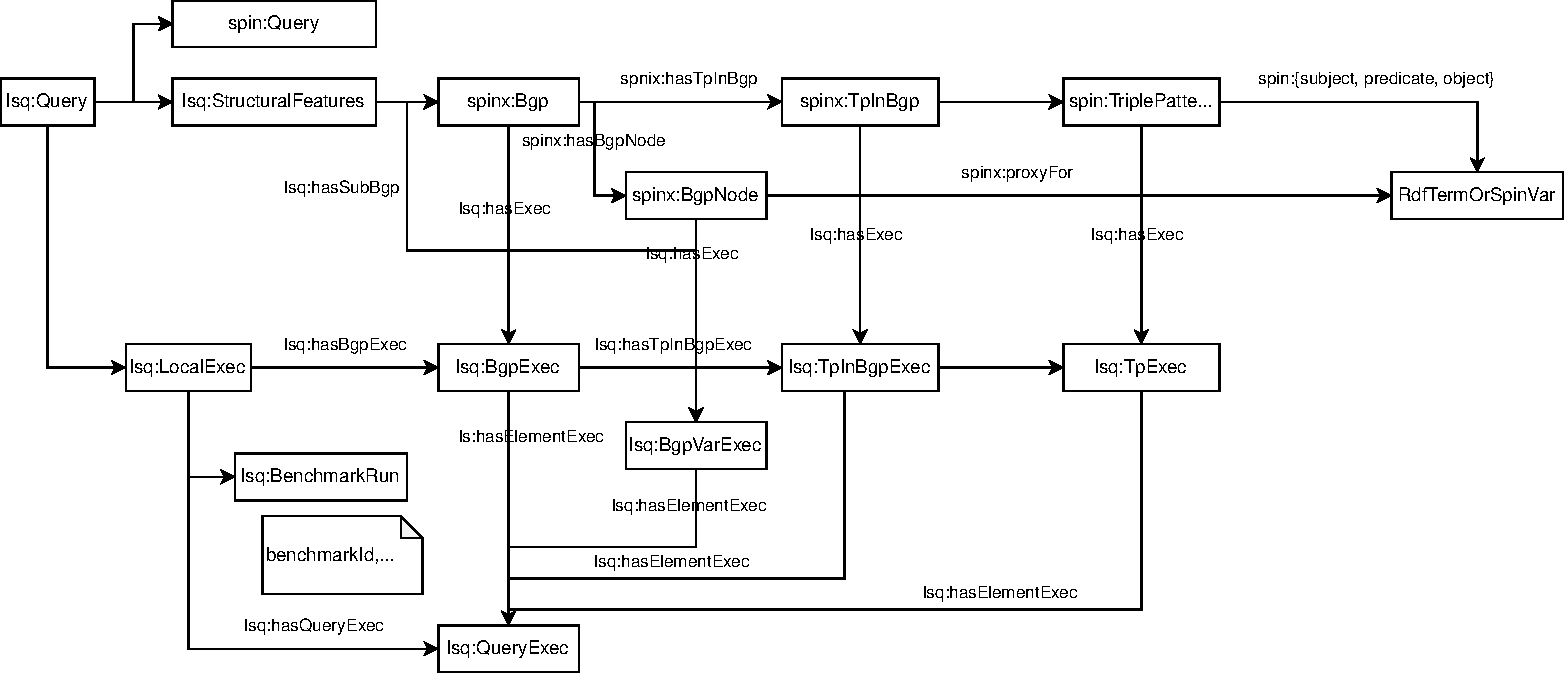
\includegraphics[width=\linewidth]{img/lsq2-datamodel}
%\caption{An overview of the LSQ data model, showing how different classes connect through different (object) properties}
%\label{fig:data_model}
%\end{figure*}

%\begin{comment}
\begin{figure*}
\centering
\begin{tikzpicture}[scale=0.73, every node/.style={transform shape}]

\tikzset{
	iri/.style={
		draw=black!50!white, 
		rectangle,
           	rounded corners,
           	thick,
           	text centered,
		top color=white, 
		bottom color=black!15, 
		font=\tt\small\hsp,
		inner sep=5pt,
		outer sep=0pt},
	lit/.style={
		draw=black!50!white, 
		rectangle,
		thick,
		text centered,
		top color=white, 
		bottom color=black!15, 
		font=\tt\small\hsp},
	arrout/.style={
		->,
		-latex,
		font=\tt\footnotesize\hsp},
	arrin/.style={
           	<-,
           	latex-,
		font=\tt\footnotesize\hsp}
}

\node[iri,anchor=center] (q) {
	\begin{tabular}{@{}l@{}}
	\multicolumn{1}{c}{lsqv:Query} \\
	\fbox{
	{\scriptsize
	\begin{tabular}{@{}l@{~~}l@{}}
	 lsqv:hash & (xsd:string)\\
	 lsqv:text & (xsd:string) \\
 	 lsqv:parseError & (xsd:string)
	\end{tabular}
	}
	}
	\end{tabular}
    };

\node[iri,anchor=center,below=3cm of q.center] (le) {lsqv:LocalExec}
 edge[arrin] node[fill=white,xshift=-0.4cm,pos=0.3] {lsqv:hasLocalExec} (q);
 
\node[iri,left=2.3cm of le.north west,anchor=north east] (re) {	
	\begin{tabular}{@{}l@{}}
	\multicolumn{1}{@{}c@{}}{lsqv:RemoteExec} \\
	\fbox{
		{\scriptsize
			\begin{tabular}{@{}l@{~~}l@{}}
			prov:atTtime & (xsd:dateTimeStamp) \\
			lsqv:hostHash & (xsd:string)
			\end{tabular}
		}
	}
	\end{tabular}}
  edge[arrin] node[fill=white] {lsqv:hasRemoteExec} (q);
  
\node[iri,anchor=center,below=2cm of re.center,dotted] (end) {cogs:Endpoint}
	edge[arrin] node[fill=white] {lsqv:endpoint} (re);

\node[iri,right=2cm of le.north east,anchor=north west] (sf) {
	\begin{tabular}{@{}l@{}}
	\multicolumn{1}{@{}c@{}}{lsqv:StructuralFeatures} \\
	\fbox{
		{\scriptsize
			\begin{tabular}{@{}l@{~~}l@{}}
			lsqv:bpgCount & (xsd:integer) \\			
			lsqv:joinVertexCount & (xsd:integer) \\
			lsqv:joinVertexDegreeMean & (xsd:decimal) \\
			lsqv:joinVertexDegreeMedian & (xsd:integer) \\
			lsqv:projectVarCount & (xsd:integer) \\
			lsqv:tpCount & (xsd:integer) \\
			lsqv:tpInBgpCountMax & (xsd:integer) \\
			lsqv:tpInBgpCountMean & (xsd:integer) \\			
			lsqv:tpInBgpCountMedian & (xsd:integer) \\			
			lsqv:tpInBgpCountMin & (xsd:integer) \\
			\end{tabular}
		}
	}
	\end{tabular}
	}
    edge[arrin] node[fill=white] {lsqv:hasStructuralFeatures} (q);
    
\node[iri,anchor=center,below=2cm of sf,dotted,xshift=4cm] (f) {sd:Feature}
	edge[arrin] node[fill=white] {lsqv:usesFeature} (sf);

\node[iri,anchor=center,below=2cm of sf] (bgp) {lsqv:Bgp}
	edge[arrin] node[fill=white] {lsqv:hasBgp} (sf);
	
\node[iri,anchor=center,left=2.4cm of bgp] (bgpe) {lsqv:BgpExec}
	edge[arrin] node[fill=white,pos=0.55] {lsqv:hasExec} (bgp);
	
%\node[iri,anchor=center,below=2cm of bgp] (ver) {...}
%	edge[arrin] node[fill=white] {lsqv:hasBgpNode} (bgp);

\node[iri,right=1cm of sf.north east,anchor=north west] (sq) {sp:Query}
 edge[arrin] node[fill=white,pos=0.6] {lsqv:hasSpin} (q);

\node[iri,anchor=center,below=1.3cm of sq.center,dotted] (t) {\begin{tabular}{@{}c@{}}sp:Select\\sp:Ask\\sp:Describe\\sp:Construct\end{tabular}}
  edge[arrout,dashed] node[auto] {} (sq);
  
\node[iri,anchor=center,below=3.75cm of le.center,xshift=-6cm] (e) {
	\begin{tabular}{@{}l@{}}
	\multicolumn{1}{@{}c@{}}{lsqv:QueryExec} \\
	\fbox{
		{\scriptsize
			\begin{tabular}{@{}l@{~~}l@{}}
			lsqv:countingDuration & (xsd:decimal) \\
			lsqv:evalDuration & (xsd:decimal) \\
			lsqv:resultCount & (xsd:integer) \\
			lsqv:serializedResult & (xsd:string) \\			
			prov:atTtime & (xsd:dateTimeStamp)
			\end{tabular}
		}
	}
	\end{tabular}
	}
    edge[arrin] node[fill=white,pos=0.4] {lsqv:hasQueryExec} (le)
    edge[arrin] node[fill=white,pos=0.55,inner sep=2pt] {lsqv:hasElementExec} (bgpe);

\node[iri,anchor=center,xshift=1.4cm] (act) at (le|-end) {
	lsqv:BenchmarkRun}
   edge[arrin] node[fill=white] {lsqv:benchmarkRun} (le);   
    
%\node[iri,anchor=center,left=4cm of sf] (bgp) { lsqv:Bgp }
%  edge[arrin] node[fill=white] {lsqv:hasBgp} (sf);
%
%\node[iri,anchor=center,above=4cm of bgp,xshift=-2cm] (ver) { lsqv:Edge }
%  edge[arrin] node[fill=white] {lsqv:hasBgpNode} (bgp);
%
%\node[iri,anchor=center,above=4cm of bgp,xshift=2cm] (tp) { lsqv:Tp }
%  edge[arrin] node[fill=white] {lsqv:hasTp} (bgp);
  
%\node[iri,anchor=center,below=1.5cm of jv.center] (t) {\begin{tabular}{@{}c@{}}lsqv:Star\\lsqv:Path\\lsqv:Hybrid\\lsqv:Sink\end{tabular}}
%edge[arrout,dashed] node[auto] {} (jv);     
    

  
\node[font=\scriptsize\tt,dashed,draw,anchor=north east] (pre) at (sq.east|-q.north)
{\begin{tabular}{@{$\!$}l@{~}l@{$\!$}} %
dct: & http://purl.org/dc/terms/\\
lsqv: & http://lsq.aksw.org/vocab\#\\ %
prov: & http://www.w3.org/ns/prov\#\\
sd: & http://www.w3.org/ns/sparql-service-description\#\\ %
sp: & http://spinrdf.org/sp\# %
\end{tabular}};
\end{tikzpicture}

%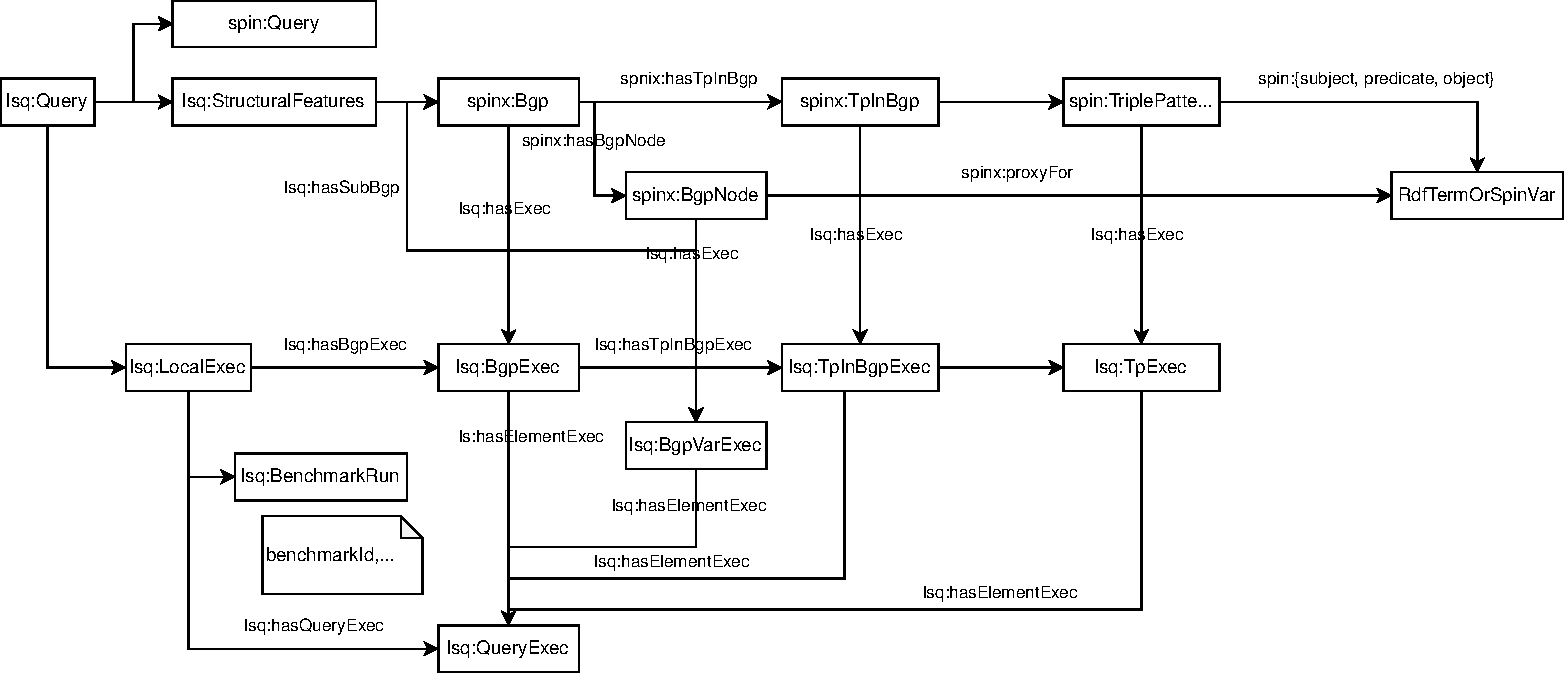
\includegraphics[width=\linewidth]{img/lsq2-datamodel}
\caption{Core of the LSQ data model: dashed lines indicate sub-classes; datatype properties are embedded within their associated class nodes to simplify presentation; external classes are shown with dotted borders. For clarity, we do not show details of the SPIN representation, or the execution of query elements more fine-grained than BGPs (which follow a similar pattern)}
\label{fig:data_model}
\end{figure*}
%\end{comment}

\begin{lstlisting}[caption = {An example LSQ/RDF representation of a SPARQL query in Turtle syntax},label = {lst:reprsentation},style=lst,basicstyle={\scriptsize\ttfamily},language=ttl,frame={single},breaklines=true,stepnumber=0,float=*]
@prefix rdf:	<http://www.w3.org/1999/02/22-rdf-syntax-ns#> .
@prefix lsqr:	<http://lsq.aksw.org/> .
@prefix lsqv:	<http://lsq.aksw.org/vocab#> .
@prefix rdfs:	<http://www.w3.org/2000/01/rdf-schema#> .
@prefix swc:	<http://data.semanticweb.org/ns/swc/ontology#> .
@prefix swr:	<http://data.semanticweb.org/> .
@prefix xsd:	<http://www.w3.org/2001/XMLSchema#> .
@prefix prov:	<http://www.w3.org/ns/prov#> .

# Primary resource describing the query found with the SWDF logs
lsqr:lsqQuery-3wBd2uKotB_-vUxnngs6ZNsGPhJmIDD9c7ig0UI24y8	
	lsqv:hasLocalExec lsqr:localExec-v9fBp3ElS1aVXXN1Z8zX1jxcHX3iy-axTgRrU2c7NY8 ;
	lsqv:hasRemoteExec lsqr:re-data.semanticweb.org-sparql_2014-05-22T16:08:17Z ,
		lsqr:re-data.semanticweb.org-sparql_2014-05-20T13:24:13Z ;
	lsqv:hasStructuralFeatures lsqr:lsqQuery-3wBd2uKotB_-vUxnngs6ZNsGPhJmIDD9c7ig0UI24y8-sf ;
	lsqv:hash "3wBd2uKotB_-vUxnngs6ZNsGPhJmIDD9c7ig0UI24y8" ;
	lsqv:text """PREFIX  rdf:  <http://www.w3.org/1999/02/22-rdf-syntax-ns#>
	               PREFIX  swc:  <http://data.semanticweb.org/ns/swc/ontology#>
	               SELECT DISTINCT  ?prop
	               WHERE { ?obj  rdf:type swc:SessionEvent ; ?prop ?targetObj FILTER isLiteral(?targetObj)  }
	               LIMIT   150""" .

# Static features of the query
lsqr:lsqQuery-3wBd2uKotB_-vUxnngs6ZNsGPhJmIDD9c7ig0UI24y8-sf	
	lsqv:bgpCount 1 ;
	lsqv:hasBgp lsqr:bgp-_x9Mckke-V9R3ddISuw-Nj_j278nT5HwiA1WUNk7tgY ;
	lsqv:joinVertexCount 1 ;
	lsqv:joinVertexDegreeMean 2 ;
	lsqv:joinVertexDegreeMedian 2 ;
	lsqv:projectVarCount 1 ;
	lsqv:tpCount 2 ;
	lsqv:tpInBgpCountMax 2 ;
	lsqv:tpInBgpCountMean 2 ;
	lsqv:tpInBgpCountMedian 2 ;
	lsqv:tpInBgpCountMin 2 ;
	lsqv:usesFeature lsqv:fn-isLiteral , lsqv:Select , lsqv:Limit , lsqv:Functions , lsqv:Group , lsqv:Filter , 
		lsqv:Distinct , lsqv:TriplePattern .              

# Remote execution no. 1 on the original endpoint
lsqr:re-data.semanticweb.org-sparql_2014-05-22T16:08:17Z	
	prov:atTime "2014-05-22T16:08:17Z"^^xsd:dateTime ;
	lsqv:endpoint swr:sparql ;
	lsqv:hostHash "O5UQpDtofxAsrJk7yzGfDolFGylMFw5446KcRZDcBkU" .

# Remote execution no. 2 on the original endpoint
lsqr:re-data.semanticweb.org-sparql_2014-05-20T13:24:13Z	
	prov:atTime "2014-05-20T13:24:13Z"^^xsd:dateTime ;
	lsqv:endpoint swr:sparql ;
	lsqv:hostHash "7aPNvqsgizRuEjH7_cO_dXoqLk-exKJ-xFmbCH3ew_E" .

# Local execution to extract statistics
lsqr:localExec-v9fBp3ElS1aVXXN1Z8zX1jxcHX3iy-axTgRrU2c7NY8-xc	
	lsqv:benchmarkRun lsqr:xc-swdf_2020-09-23_at_23-09-2020_17:10:19 ;
	lsqv:hasQueryExec lsqr:queryExec-Cmv7SccybbBxwkep_cHvDiF3piq29tH7NWlDfIiCHqU .

# Results of local execution
lsqr:queryExec-Cmv7SccybbBxwkep_cHvDiF3piq29tH7NWlDfIiCHqU	
	prov:atTime "2020-09-23T15:27:36.325Z"^^xsd:dateTime ;
	lsqv:countingDuration 0.008466651 ;
	lsqv:evalDuration 0.008868635 ;
	lsqv:resultCount 16 .
		
# The full data further include a SPIN description of the query, a list of BGPs within the query,
# a list of triple patterns and terms within the query, as well as execution statistics for individal
# BGPs, triple patterns and sub-BGPs induced by join variables
\end{lstlisting}

In Figure~\ref{fig:data_model} we provide an overview of the model used to represent queries in RDF, while in Listing~\ref{lst:reprsentation} we provide a snippet of the top-level data generated for a query found in the \swdf logs.\footnote{Note that for the purposes of presentation, we abbreviate some of the details of the query, including the IRIs used to identify local query executions.} We now discuss the groups of features described for each query.

\paragraph{Query instance} We define a ``query'' to be uniquely identified by the syntactic query string (independently of the endpoint, the particular execution, etc.). We type these queries with \texttt{lsqv:Query}. Instances of this class are linked to the query string using \texttt{lsqv:text}, and to various instances of local and remote executions. Other links are provided to other resources that capture further details of the static features of the query, its structure, as well as runtime statistics of its local execution (on our server) as information about its remote execution (on the original server).

\paragraph{Static features} Next we define some static features of the query, independent of the dataset over which it is evaluated. These include links to its individual join variables, triple patterns, and basic graph patterns; the SPARQL features that is uses; its number of projected variables, basic graph patterns, join variables, triple patterns; the maximum, mean and median degree of its join variables; and the maximum and minimum size of its basic graph patterns. The triple patterns and basic graph patterns themselves link to the SPIN representation of the query included in the description (and discussed presently); the triple patterns, in turn, link to the resources used by the query. The join variables, on the other hand, are described separately, indicating the degree of the variable and type of join~\cite{SaleemN14} it induces.

\paragraph{SPIN representation} While the static features aim to capture some high-level descriptions of the query that may be of interest to specific use cases, some details may be missing. In the interest of generality, we also include for each query a SPARQL Inferencing Notation (SPIN)~\cite{spin} representation of the query, which essentially captures a fine-grained translation of the SPARQL query to RDF. This SPIN encoding can be translated back to a SPARQL query equivalent to the original.\footnote{Given a query $Q$ and dataset $D$, let $Q(D)$ denote the result(s) of evaluating $Q$ over $D$. Two queries $Q_1$ and $Q_2$ are then defined to be \textit{equivalent} if and only if $Q_1(D) = Q_2(D)$ for every dataset $D$.} 

%Note that while Listing~\ref{lst:reprsentation} provides an example of the SPIN notation, for clarity, the model shown in Figure~\ref{fig:Schema} excludes most of the SPIN vocabulary, including onle some of the high-level sub-classes that indicate \texttt{SELECT}, \texttt{CONSTRUCT}, \texttt{ASK} and \texttt{DESCRIBE} queries.

\paragraph{Remote execution(s)} Next, individual queries are associated with one or more executions on the original endpoint, including a timestamp of when the query was executed, as well as an anonymised ID for the client---based on their cryptographically-hashed and salted I.P.---to identify which queries are run by the same agent.\footnote{A ``salt'' in cryptography is a privately-held arbitrary string that is combined (e.g., concatenated) with the input being hashed in order to avoid attacks based on precomputed tables (e.g., of common values or, in this case, of a collection of I.P.'s of interest).} The remote execution is also linked to the originating endpoint using \texttt{lsqv:endpoint}.\footnote{Although there exist properties called ``endpoint''---such as \texttt{void:sparqlEndpoint} or \texttt{sd:endpoint}---the domains of these properties were not query executions, but rather VoID datasets (i.e., sets of RDF triples), or SPARQL services. Though it would be possible to define properties such as \texttt{lsqv:dataset} or \texttt{lsqv:service} and then link a query execution \texttt{<x>} to an endpoint URL \texttt{<e>} with \texttt{<x> lsqv:dataset [ void:sparqlEndpoint <e> ]}, or alternatively \texttt{<x> lsqv:service [ sd:endpoint <e> ]}, this would introduce $O(n)$ additional triples to the LSQ~2.0 dataset, for $n$ the number of remote query executions (in LSQ~2.0, $n = 43,952,379$). (Please note that the dataset or service may change during the lifetime of the log, which we do not have information about; hence we cannot refer to one dataset/service at a given endpoint.) Thus we rather introduce \texttt{lsqv:endpoint} in the data and define property chain axioms in the LSQ~2.0 vocabulary to relate \texttt{lsqv:endpoint} to \texttt{lsqv:dataset}/\texttt{void:sparqlEndpoint} and \texttt{lsqv:service}/\texttt{sd:endpoint}.} Given that these meta-data constitute provenance for the query, we use the PROV Ontology (PROV-O)~\cite{prov-o} for modelling the time, date and agent involved in the remote execution.

\paragraph{Local execution} In most cases, the log of the remote executions will not provide statistics about the execution of the query in terms of how many results were returned, how long it took, how selective were the individual patterns, and so forth. Hence we re-execute the queries offline against the original dataset to generate runtime statistics about the query. Local executions were run on a machine with 64 core Intel(R) Xeon(R) CPU E5-2683 v4 @ 2.10GHz, and 528 GB RAM running Ubuntu 18.04.5 LTS using Virtuoso 7.2.\footnote{The configuration used for Virtuoso was \texttt{MaxQueryMem = 32G}, \texttt{NumberOfBuffers = 20050000}, and \texttt{MaxDirtyBuffers = 20000000}.} Due to the large number of queries to evaluate, we set a query timeout of one minute. The statistics generated include the number of results and the runtime for the query, as well as the number of results and the selectivity for each individual triple pattern.\footnote{The selectivity of the triple pattern is the ratio of triples from the dataset that it selects.} Runtime statistics are computed in a controlled environment that abstract away external factors such as the load on the endpoint server, etc.; however, due to the costs involved in evaluating such queries, we compute these only for one query engine, namely Virtuoso~7.2, where runtime estimates may thus vary for other engines.

\paragraph{Summary} The meta-data described in this section aim to strike a balance in terms of the four desiderata mentioned previously. In terms of \textbf{Generality}, we provide detailed meta-data for static query features, for provenance, and for runtime query statistics. In terms of \textbf{Conciseness}, though the detailed meta-data do require potentially many triples to be encoded for each query, we take steps to reduce this number by re-using resources insofar as appropriate where, for example, each unique query string is encoded once per log, with one set of static features, one SPIN representation, and one set of local executions, being subsequently linked to its different remote executions (rather than duplicate the former meta-data each time the same query string appears in the log). In terms of \textbf{Usability}, we provide some ``shortcut triples'' that allow for quickly finding queries of interest; for example, the static features of the query are largely of this form, where all such meta-data could in principle be computed from the SPIN representation, but using rather complex SPARQL queries over LSQ; the static query features are thus presented to make it easier to find queries, for example, with a certain range of numbers of triple patterns, or queries using \texttt{DISTINCT} and \texttt{GROUP BY}, etc. We will discuss \textbf{Linked Data Compatibility} in the section that follows.

\section{Publication}\label{sec:publish}

The LSQ dataset is published as Linked Data. Before describing the current contents of LSQ, we discuss in more detail how LSQ has been published.

\paragraph{Access Methods} We provide a number of ways to access LSQ. Firstly, following Linked Data principles, all IRIs under the \texttt{lsqr:} namespace are made dereferenceable using a \texttt{303 Redirect}; this is implemented with LodView\footnote{https://github.com/LodLive/LodView} and supports content negotiation. A SPARQL endpoint is provided for querying LSQ~2.0. Table~\ref{tab:access} lists the locations for these access methods.

\begin{table*}
\centering
\setlength\columnsep{10pt}
\setlength{\tabcolsep}{3ex}
\caption{Locations from which LSQ can be accessed including an example Linked Data IRI, the vocabulary, dumps, the SPARQL endpoint, as well as locations where LSQ is indexed, including DataHub, Linked Open Vocabularies (LOV) and prefix.cc}
\label{tab:access}
\begin{tabular}{l@{~~~}l}
\toprule
\textbf{Method} & \textbf{Location}\\
\midrule
Linked Data IRIs & \url{http://lsq.aksw.org/lsqQuery-3wBd2uKotB_-vUxnngs6ZNsGPhJmIDD9c7ig0UI24y8} (\textit{example}) \\
Vocabulary & \url{http://lsq.aksw.org/vocab} \\
Dumps       	 & \url{http://lsq.aksw.org/downloads} \\
SPARQL Endpoint  & \url{http://lsq.aksw.org/sparql} \\
\midrule
\textbf{Catalogue} & \textbf{Location}\\
\midrule
Datahub		& \url{https://datahub.io/dataset/lsq} \\
LOV			& \url{https://lov.linkeddata.es/dataset/lov/vocabs/lsq} \\
prefix.cc	& \url{http://prefix.cc/lsqv} \\
\bottomrule
\end{tabular}
\end{table*}

\paragraph{Vocabulary} As seen in Figure~\ref{fig:data_model}, we use a mixture of a custom vocabulary in the \texttt{lsqv:} namespace, as well as existing vocabulary where possible. The custom LSQ vocabulary dereferences (via \texttt{303 Redirect}) to an RDFS/OWL definition of the corresponding terms in Turtle, which includes metadata about authors. The vocabulary meets four of the five stars of Linked Data vocabulary use~\cite{JanowiczHAKV14}.\footnote{With respect to the fifth star, which requires that our LSQ vocabulary be \textit{linked to} from external vocabularies, we are not aware of such links, though we do know, for example, that Varga et al.~\cite{varga2018analytical} incorporate elements of the LSQ vocabulary within their own Analytical Metadata (AM) model, while Singh et al.~\cite{singh2019qaldgen} also use the LSQ vocabulary within their benchmark.} With respect to external vocabulary, we re-use terms from the SPARQL Inferencing Notation (SPIN) ontology~\cite{spin}, as well as the Provenance Ontology (PROV-O)~\cite{prov-o} where possible.%\footnote{We have avoided re-using inappropriate terms. For example, we use \texttt{lsqv:endpoint} rather than \texttt{void:sparqlEndpoint} or \texttt{sd:endpoint} as the former has a query execution as its domain, while the latter have a dataset and a service as their domain, respectively.}

\paragraph{Discoverability} The LSQ dataset has been registered in the DataHub catalogue, while the LSQ vocabulary has been listed on Linked Open Vocabularies (LOV)~\cite{VandenbusscheAP17} as well as prefix.cc. We provide these locations in Table~\ref{tab:access}. We also compute and publish meta-data about the LSQ dataset using the Vocabulary of Interlinked Datasets (VoID)~\cite{key:void}. More specifically, we compute a separate VoID description for each log and make the resulting description accessible via both a downloadable file and a named graph of the SPARQL endpoint.

\paragraph{Availability} The LSQ dataset has been hosted for over six years (at the time of writing) by the Agile Knowledge Engineering and Semantic Web (AKSW) group. As discussed in Section~\ref{sec:lsq_adoption}, it has been widely adopted in that time. The dataset is available to all under a CC-BY license. We further make the source code used for generating the LSQ dataset from the raw query logs available on Github \url{https://github.com/AKSW/LSQ}.

\section{LSQ~2.0 Logs}\label{sec:logs}

We now describe the content of the LSQ~2.0 dataset. In order to collect raw SPARQL query logs, we sent mails both to the \texttt{public-lod@w3.org} mailing list and to individual providers of endpoints. We also incorporated logs from LSQ~1.0~\cite{SaleemAHMN15} and a sample of queries from the Wikidata logs~\cite{MalyshevKGGB18}. We thus acquired access to the logs of 27 endpoints, 22 of which are part of Bio2RDF release 3~\cite{DumontierCCAEBD14}.\footnote{We also acquired logs for the British Museum and UniProt endpoints, but decided to omit them due to having few unique queries.} Table~\ref{tab:dsbstats} provides high-level statistics of the query logs from which we extract the LSQ dataset, including the query executions registered; the unique query strings; the number of queries providing a runtime error, or returning zero results; as well as the percentage of unique queries using \texttt{SELECT}, \texttt{CONSTRUCT}, \texttt{DESCRIBE} or \texttt{ASK}. Aside from the initial log of LSQ, only one log is already publicly available, namely Wikidata~\cite{MalyshevKGGB18}, of which we include a subset described in our data model.


% In Table~\ref{tab:lsqstats}, we provide statistics of the dataset over which the queries were executed, including the unique subjects, predicates, objects and triples per dataset, as well as the location of the SPARQL endpoint. 
  
\paragraph{\affymetrix} is a biomedical Linked Dataset describing probesets found in DNA microarrays~\cite{DumontierCCAEBD14}.

\paragraph{\biomodels} is a biomedical Linked Dataset describing mathematical models of biological systems~\cite{DumontierCCAEBD14}.\footnote{The external SPARQL endpoint is spelt \texttt{biomedels}, and thus the IRIs use this spelling in LSQ~2.0.}

\paragraph{BioPortal} is a biomedical Linked Dataset cataloguing biomedical ontologies~\cite{DumontierCCAEBD14}.

\paragraph{\ctd: Comparative Toxicogenomics Database} is a biomedical Linked Dataset that describes how environmental chemicals relate to diseases~\cite{DumontierCCAEBD14}.

\paragraph{\dbpedia} is a cross-domain Linked Dataset that is primarily extracted from Wikipedia~\cite{LehmannIJJKMHMK15}.

\paragraph{\dbsnp: Single Nucleotide Polymorphism Database} is a biomedical Linked Dataset that describes single base nucleotide substitutions and short deletion and insertion polymorphisms~\cite{DumontierCCAEBD14}.

\paragraph{\drugbank} is a biomedical Linked Dataset that describes drugs and drug targets~\cite{DumontierCCAEBD14}.

\paragraph{\genage} is a biomedical Linked Dataset that describes human and other genes linked with ageing~\cite{DumontierCCAEBD14}.

\paragraph{\gendr: Dietary Restriction Gene Database} is a biomedical Linked Dataset that describes genes associated with dietary restrictions~\cite{DumontierCCAEBD14}.

\paragraph{\go: Gene Ontology} is a biomedical ontology that describes gene, gene products, and their functions~\cite{DumontierCCAEBD14}.

\paragraph{\goa: Gene Ontology Annotation} is a biomedical Linked Dataset that provides annotations on proteins, RNA and protein complexes~\cite{DumontierCCAEBD14}.

\paragraph{\hgnc: HUGO Gene Nomenclature Committee} is a biomedical Linked Dataset that describes human gene nomenclature~\cite{DumontierCCAEBD14}.

\paragraph{\irefindex} is a biomedical Linked Dataset that indexes interaction data for proteins~\cite{DumontierCCAEBD14}.

\paragraph{\kegg: Kyoto Encyclopedia of Genes and Genomes} is a biomedical Linked Dataset that describes functions of genes and biological systems~\cite{DumontierCCAEBD14}.

\paragraph{\linkedgeodata} is a geographical Linked Data extracted primarily from Open Street Map~\cite{StadlerLHA12}.

\paragraph{\linkedspl: Linked Structured Product Labelling} is a biomedical Linked Dataset that contains meta-data about drug labels sourced from DailyMed~\cite{DumontierCCAEBD14}.

%\paragraph{Life Science Resource Registry (LSR)} is a biomedical Linked Dataset that contains terminological resources relating to the life sciences~\cite{DumontierCCAEBD14}. \ah{No longer in Table 2} \ah{Not in the endpoint.}

%\paragraph{Medical Subject Headings (MeSH)} is a biomedical Linked Dataset that describes a taxonomy for cataloguing biomedical information~\cite{DumontierCCAEBD14}. \ah{No longer in Table 2} \ah{Not in the endpoint.}

\paragraph{\mgi: Mouse Genome Informatics} is a biomedical Linked Dataset that describes mouse genes, alleles, and strains~\cite{DumontierCCAEBD14}.

\paragraph{NCBI Gene} is a biomedical Linked Dataset that describes gene-related information given by the National Center for Biotechnology Information (NCBI)~\cite{DumontierCCAEBD14}.

%\paragraph{National Drug Code (NDC)} is a biomedical Linked Dataset that describes unique product identifiers for drugs intended for human consumption in the United States~\cite{DumontierCCAEBD14}. %\ah{stats} 
%\ah{No longer in Table 2.} \ah{Not in the endpoint.}

\paragraph{Online Mendelian Inheritance in Man (\omim)} is a biomedical Linked Dataset that catalogues human genes as well as genetic traits and disorders~\cite{DumontierCCAEBD14}. %\ah{stats}

%\paragraph{Orphanet} is a biomedical Linked Dataset that describes rare diseases and orphan drugs~\cite{DumontierCCAEBD14}. \ah{No longer in Table 2.} \ah{Not in the endpoint.} 

\paragraph{\pharmgkb} is a biomedical Linked Dataset describing how genetic variations impact drug responses~\cite{DumontierCCAEBD14}. %\ah{stats}

\paragraph{\sabiork: System for the Analysis of Biochemical Pathways -- Reaction Kinetics} is a biomedical Linked Dataset that describes biochemical reactions~\cite{DumontierCCAEBD14}. %\ah{stats}

\paragraph{\sgd: Saccharomyces Genome Database} is a biomedical Linked Dataset describing the biology and genetics of the yeast \textit{Saccharomyces cerevisiae}~\cite{DumontierCCAEBD14}. %\ah{stats}

\paragraph{\sider: Side Effect Resource} is a biomedical Linked Dataset describing the side effects of drugs~\cite{DumontierCCAEBD14}. %\ah{stats}

\paragraph{\swdf: Semantic Web Dog Food} is a bibliographical Linked Dataset describing papers, presentations and people participating in top Semantic Web related conferences and workshops~\cite{MollerHHD07}. 

\paragraph{\taxonomy: NBCI Taxonomy} is a biomedical Linked Dataset that describes all organisms found in genetic databases~\cite{DumontierCCAEBD14}.

\paragraph{\wikidata} is a collaboratively edited knowledge graph hosted by the Wikimedia foundation~\cite{MalyshevKGGB18}. 

\paragraph{\wormbase} is a biomedical Linked Dataset that describes the biology and genome of worms~\cite{DumontierCCAEBD14}. 

%\ah{data stats} The Semantic Web Dog Food (\swdf) log spans from May 16, 2014 to November 12, 2014 and records over 1.4 million query executions.

%\paragraph{UniProt} \ah{include?}


%\subsubsection{British Museum} provides a Linked Data representation of an online collection containing records of more than 3 million artefacts. The British Museum (BM) Linked Dataset is accessible at \url{http://collection.britishmuseum.org/sparql} through an OWLIM/GraphDB interface. The log we have acquired spans from November 8, 2014 to December 1, 2014 and contains over 800 thousand query executions.

%\subsubsection{Overview of datasets}
%In Table~\ref{tab:dsbstats}, we present some high-level statistics of the \textit{original} Linked Datasets corresponding to the time of the logs (e.g., \dbpedia refers to \dbpedia v.3.5.1), including the number of distinct triples, subjects, predicates, objects and classes over which queries would have been issued. The statistics were collected by downloading and locally analysing the data. These datasets will be used later to generate controlled estimates of data-sensitive statistics for queries, such as runtimes, result sizes, triple pattern selectivity, etc.


%\newcommand{\cenh}[1]{\multicolumn{1}{c}{#1}}




\section{LSQ~2.0 Query Statistics}\label{sec:queries}

We now look in more detail at the composition of the queries currently included in the LSQ dataset. In particular, we first look at some high-level statistics for queries in the dataset, before looking at the static features of the query, the agents making the queries, as well as runtime statistics computed against the corresponding dataset. Finally we discuss the composition of the LSQ dataset itself.

%We applied the RDFisation process to the four logs mentioned in the previous section. Given that the logs were in different formats, we created custom scripts to extract and normalise data from the four different sources, mapping them to the target schema outlined in Section~\ref{sec:model}. We now give a more in-depth analysis of the resulting datasets, as well as an analysis of the unique queries, query executions and agents mentioned therein. Our goal is to provide insights into the scope and usefulness of the dataset, as well as its limitations.




%Bullets for Aidan from Mario report
%\begin{itemize}
%\item 2 datasets DBLP and \swdf 5 million and 2 million queries respectively.
%\item Select most common used operator 96.9 in \dbpedia , ask 1.6 construct 1.5 and describe .002 , In \swdf select is 99.7
%\item Filter most common operator 49 percent both
%\item Lang most used function only in \dbpedia and obvious because of it support for multiple languages, second most used function is EQUAL (dblp 23 percent) and \swdf top most 93 percent.
%\item Distinct more popular on \dbpedia than \swdf
%\item lack of usage of features like Order BY, GRAPH, FROM , FROM NAMED and OFFSET
%\item UNION is 11.84 for \dbpedia while for OPTIONAL they said significant
%\item triple pattern number, 66 percent in \dbpedia and 97.25 in \swdf contain a single triple pattern
%\item 6 types of joins , SS, SO, SP, PP, PO, OO . SS is most used almost 60 $\%$ in both while SO is second most common around 35 while OO is almost 5, rest are negligible. 
%\end{itemize}

\paragraph{High-level statistics:} Table~\ref{tab:dsbstats} provides a high-level analysis of the queries (both query executions and unique queries) appearing in each of the logs considered. From the overall row, we see that LSQ contains 43.95 million query executions and 11.56 million unique queries, implying that each query is executed, on average, 3.8 times within each log. Of the unique queries, 7.7 million (66.9\%) have runtime errors; and 2.3 million (20.0\%) have no errors but return empty results. A high ratio of runtime errors come from the Bio2RDF logs. The majority of queries are \texttt{CONSTRUCT} queries (60.0\%), followed by \texttt{SELECT} (32.3\%), \texttt{DESCRIBE} (7.1\%) and \texttt{ASK} (0.5\%). We find that \texttt{CONSTRUCT} queries are particularly prevalent on Bio2RDF endpoints, while \texttt{DESCRIBE} queries are particularly prevalent on \dbpedia and Wikdata endpoints, possibly due to the use of such queries for dereferencing Linked Data IRIs through the endpoint.

\newcommand{\cenh}[1]{#1}

\begin{table*}
\setlength{\tabcolsep}{1.3ex}
\centering
\caption{High-level statistics for queries in the LSQ dataset (QE = Query Executions, UQ = Unique Queries, RE = Runtime Error, ZR = Zero Results, \texttt{SEL} = \texttt{SELECT}, \texttt{CON} = \texttt{CONSTRUCT}, \texttt{DES} = \texttt{DESCRIBE})}
\label{tab:dsbstats}
\begin{tabular}{lrrrrrrrr}
\toprule
\textsc{Dataset} & \cenh{\textsc{QE}} & \cenh{\textsc{UQ}} & \cenh{\textsc{RE}} & \cenh{\textsc{ZR}} & \cenh{\textsc{\texttt{SEL} (\%)}} & \cenh{\textsc{\texttt{CON} (\%)}} & \cenh{\textsc{\texttt{DES} (\%)}} & \cenh{\textsc{\texttt{ASK} (\%)}} \\
\midrule
\affymetrix	&	1,229,339	&	311,096	&	277,983	&	31,659	&	16.47	&	83.21	&	0.02	&	0.30	\\
\biomodels	&	1,238,375	&	435,232	&	412,984	&	21,692	&	41.18	&	58.75	&	0.00	&	0.06	\\
BIOPORTAL	&	1,337,804	&	89,664	&	85,273	&	3,389	&	64.88	&	34.78	&	0.00	&	0.34	\\
\ctd	&	940,390	&	287,296	&	266,999	&	19,824	&	11.98	&	87.76	&	0.00	&	0.26	\\
\dbpedia	&	6,535,500	&	4,258,941	&	1,259,972	&	1,755,338	&	69.90	&	3.59	&	25.23	&	1.28	\\
\dbsnp	&	794,023	&	269,498	&	267,662	&	1,698	&	4.99	&	94.99	&	0.00	&	0.02	\\
\drugbank	&	1,613,951	&	379,233	&	372,022	&	6,186	&	46.67	&	52.80	&	0.05	&	0.48	\\
\genage	&	589,211	&	265,067	&	263,205	&	1,661	&	5.55	&	94.43	&	0.00	&	0.02	\\
\gendr	&	690,864	&	270,697	&	262,776	&	7,726	&	7.53	&	92.45	&	0.00	&	0.02	\\
\go	&	1,839,991	&	121,542	&	88,743	&	30,082	&	98.31	&	0.03	&	0.35	&	1.31	\\
\goa	&	3,544,273	&	343,836	&	310,800	&	32,317	&	26.18	&	73.69	&	0.06	&	0.07	\\
\hgnc	&	1,529,681	&	364,961	&	327,540	&	33,568	&	29.15	&	70.58	&	0.04	&	0.23	\\
%HOMOLOGENE	&	1,242,694	&	321,061	&	1765	&	0	&	0.00	&	0.00	&	0.00	&	0.00	\\
\irefindex	&	1,560,704	&	309,777	&	289,546	&	19,858	&	18.10	&	81.88	&	0.00	&	0.02	\\
\kegg	&	66,830	&	19,871	&	10,386	&	8,004	&	92.04	&	4.30	&	0.41	&	3.24	\\
\linkedgeodata	&	154,884	&	61,897	&	11,028	&	13,990	&	98.58	&	1.00	&	0.02	&	0.40	\\
\linkedspl	&	337,001	&	204,112	&	203,534	&	310	&	0.28	&	99.69	&	0.00	&	0.03	\\
\mgi	&	1,316,673	&	319,627	&	277,080	&	33,781	&	21.12	&	78.60	&	0.05	&	0.23	\\
\ncbigene	&	770,716	&	216,832	&	215,938	&	718	&	8.71	&	91.26	&	0.00	&	0.04	\\
\omim	&	1,506,621	&	335,541	&	290,483	&	44,093	&	22.78	&	76.89	&	0.08	&	0.26	\\
\pharmgkb	&	94,540	&	24,000	&	14,597	&	8,649	&	60.35	&	39.65	&	0.00	&	0.01	\\
\sabiork	&	922,407	&	274,098	&	253,733	&	19,938	&	7.91	&	92.07	&	0.00	&	0.02	\\
\sgd	&	973,281	&	318,641	&	309,593	&	7,199	&	16.06	&	80.53	&	0.30	&	3.12	\\
\sider	&	599,285	&	277,766	&	274,963	&	1,965	&	9.38	&	90.59	&	0.00	&	0.03	\\
\swdf	&	1,415,567	&	101,423	&	30,792	&	36,789	&	73.57	&	0.06	&	26.17	&	0.21	\\
\taxonomy	&	7,698,898	&	354,582	&	334,290	&	20,041	&	15.83	&	84.16	&	0.00	&	0.02	\\
\wikidata	&	3,298,254	&	844,256	&	520,976	&	150,395	&	95.03	&	0.13	&	0.08	&	4.77	\\
\wormbase	&	1,353,316	&	498,170	&	496,325	&	1,660	&	49.33	&	50.66	&	0.00	&	0.01	\\
\midrule
Overall	&	43,952,379	&	11,557,656
		&	7,729,223	&	2,312,530	&	36.14	&	57.8	&	1.89	&	0.60	\\
\bottomrule
\end{tabular}
\end{table*}


\paragraph{Static features:} Turning to static features, we first look at the percentages of unique queries without parse errors using different SPARQL features (note that we will analyse joins in BGPs and property paths later). Table~\ref{tab:distfeatures} provides statistics for the usage of different features of SPARQL. We see that \texttt{FILTER} is among the most widely used features, along with SPARQL functions and expressions (note that almost all filters use such expressions). This feature is followed by \texttt{DISTINCT} and other solution modifiers, \texttt{UNION}, \texttt{OPTIONAL}, etc. Notably these are all SPARQL~1.0 features. The \texttt{SERVICE} keyword is commonly used on \wikidata since the Wikidata Query Service provides a custom service for retrieving multilingual labels as preferred/available.


\begin{table*}[!tb]
\setlength{\tabcolsep}{0.6ex}
\centering
\caption{Percentage of unique queries without parse errors using the specified SPARQL feature (\textsc{Sol. Mod.} includes the solution modifiers \texttt{ORDER BY}, \texttt{OFFSET}, and \texttt{LIMIT}; \textsc{Agg.} includes aggregation features \texttt{GROUP BY}, \texttt{HAVING}, \texttt{AVG}, \texttt{SUM}, \texttt{COUNT}, \texttt{MAX}, and \texttt{MIN}; \textsc{Neg.} includes \texttt{MINUS}, \texttt{NOT EXISTS}, and \texttt{EXISTS}; \textsc{Bind.} includes \texttt{VALUES} and \texttt{BINDING}; \textsc{Graph} includes \texttt{FROM}, \texttt{FROM NAMED}, and \texttt{GRAPH}; \textsc{Func.} includes SPARQL functions and expressions)} 
\label{tab:distfeatures}
\begin{tabular}{lrrrrrrrrrrrrr} \toprule
\textsc{Dataset} & \texttt{UNION} & \texttt{OPTIONAL} & \texttt{DISTINCT} & \texttt{FILTER} & \texttt{REGEX} & \texttt{SERVICE} & \textsc{Sub-Q.} & \textsc{Sol. M.} & \textsc{Agg.} & \textsc{Neg.} & \textsc{Bind.} & \textsc{Graph}  & \textsc{Func.} \\  \midrule
\affymetrix & 3.68 & 0.02 & 7.64 & 83.30 & 0.15 & 0.01 & 0.06 & 4.85 & 0.36 & 0.00 & 0.01 & 0.69 & 83.30 \\
\biomodels & 2.64 & 0.01 & 0.18 & 94.32 & 0.06 & 0.00 & 0.01 & 0.12 & 0.10 & 0.00 & 0.00 & 0.03 & 94.32 \\
BIOPORTAL & 1.50 & 0.06 & 0.05 & 37.95 & 2.23 & 0.01 & 0.01 & 0.21 & 34.10 & 0.00 & 0.00 & 34.26 & 37.95 \\
\ctd & 3.99 & 0.02 & 0.37 & 88.06 & 0.06 & 0.04 & 0.01 & 3.57 & 0.13 & 0.00 & 0.01 & 3.21 & 88.06 \\
\dbpedia & 28.68 & 19.97 & 22.22 & 29.87 & 4.10 & 0.00 & 2.22 & 8.92 & 9.98 & 0.00 & 1.11 & 0.01 & 29.87 \\
\dbsnp & 0.05 & 0.01 & 0.10 & 94.87 & 0.00 & 0.05 & 0.01 & 0.13 & 0.07 & 0.00 & 0.00 & 0.09 & 94.87 \\
\drugbank & 2.58 & 15.55 & 12.37 & 54.67 & 1.81 & 0.10 & 0.02 & 9.31 & 2.59 & 0.00 & 0.01 & 2.73 & 54.67 \\
\genage & 0.00 & 0.01 & 0.08 & 94.37 & 0.00 & 0.00 & 0.01 & 0.06 & 0.07 & 0.00 & 0.00 & 0.02 & 94.37 \\
\gendr & 0.01 & 0.01 & 0.07 & 96.55 & 0.00 & 0.01 & 0.01 & 0.06 & 0.07 & 0.00 & 0.00 & 0.02 & 96.55 \\
\go & 9.08 & 0.16 & 20.98 & 18.82 & 5.92 & 0.89 & 0.07 & 3.86 & 0.08 & 0.00 & 0.01 & 0.02 & 18.82 \\
\goa & 4.17 & 0.01 & 5.00 & 84.76 & 9.15 & 0.86 & 0.03 & 0.71 & 0.09 & 0.00 & 0.00 & 0.44 & 84.76 \\
\hgnc & 3.16 & 0.02 & 5.00 & 84.12 & 0.04 & 0.03 & 0.02 & 1.20 & 0.44 & 0.00 & 0.00 & 0.47 & 84.12 \\
\irefindex & 9.99 & 1.00 & 0.86 & 83.37 & 2.29 & 0.01 & 0.01 & 0.87 & 0.12 & 0.00 & 0.00 & 0.74 & 83.37 \\
\kegg & 11.64 & 1.13 & 54.91 & 7.22 & 2.86 & 0.07 & 0.04 & 42.95 & 1.02 & 0.00 & 0.01 & 0.79 & 7.22 \\
\linkedgeodata & 1.15 & 19.13 & 9.24 & 18.06 & 2.61 & 0.01 & 7.64 & 30.75 & 37.57 & 0.00 & 0.52 & 2.52 & 18.06 \\
\linkedspl & 0.00 & 0.01 & 0.00 & 99.76 & 0.00 & 0.00 & 0.01 & 0.05 & 0.07 & 0.00 & 0.00 & 0.03 & 99.76 \\
\mgi & 3.57 & 0.02 & 6.99 & 79.43 & 0.43 & 0.01 & 0.03 & 2.98 & 0.57 & 0.00 & 0.05 & 0.64 & 79.43 \\
\ncbigene & 0.02 & 0.01 & 0.17 & 91.53 & 0.02 & 0.03 & 0.01 & 2.72 & 0.22 & 0.00 & 0.00 & 2.61 & 91.53 \\
\omim & 3.52 & 1.10 & 4.90 & 80.83 & 0.31 & 0.39 & 0.04 & 5.62 & 0.93 & 0.00 & 0.01 & 1.09 & 80.83 \\
\pharmgkb & 33.05 & 0.00 & 42.22 & 47.92 & 0.28 & 0.13 & 0.01 & 43.40 & 0.07 & 0.00 & 0.00 & 1.14 & 47.92 \\
\sabiork & 4.15 & 0.01 & 0.12 & 92.00 & 0.00 & 0.00 & 0.01 & 0.17 & 0.09 & 0.00 & 0.00 & 0.05 & 92.00 \\
\sgd & 1.63 & 0.01 & 6.73 & 80.06 & 0.09 & 0.03 & 0.04 & 4.38 & 3.87 & 0.00 & 0.00 & 4.24 & 80.06 \\
\sider & 0.02 & 0.01 & 7.44 & 90.87 & 0.00 & 0.03 & 0.01 & 7.42 & 0.09 & 0.00 & 0.00 & 0.73 & 90.87 \\
\swdf & 40.13 & 34.08 & 53.16 & 2.34 & 0.87 & 0.04 & 0.10 & 31.45 & 1.08 & 0.00 & 0.01 & 32.32 & 2.34 \\
\taxonomy & 3.19 & 0.01 & 0.04 & 92.91 & 0.04 & 0.00 & 0.01 & 0.35 & 0.25 & 0.00 & 0.00 & 0.44 & 92.91 \\
\wikidata & 9.27 & 29.21 & 15.32 & 26.48 & 1.13 & 54.38 & 7.44 & 40.72 & 7.99 & 0.00 & 8.99 & 0.00 & 26.48 \\
\wormbase & 14.16 & 4.46 & 0.12 & 69.92 & 9.69 & 1.58 & 0.00 & 0.27 & 0.63 & 0.00 & 0.00 & 0.82 & 69.92 \\
\midrule
Overall & 7.22 & 4.67 & 10.23 & 67.57 & 1.63 & 2.17 & 0.66 & 9.14 & 3.77 & 0.00 & 0.34 & 3.34 & 67.57 \\
\bottomrule
\end{tabular}
\end{table*}

Next, in Table~\ref{tab:bgppp}, we provide three types of statistics about the basic graph patterns and property path features used. First, we present the unique number of subject, predicate and object terms used in the BGPs of the logs in order to characterise their diversity. We see that \dbpedia, \linkedgeodata and \wikidata offer the most diversity, particularly in terms of predicates found in the queries. Second, we present the percentage of queries with different types of joins in the basic graph patterns~\cite{SaleemN14}. Each join variable in a basic graph pattern is analysed in order to understand how they connect triple patterns. We say that a join vertex has an ``outgoing link'' if it appears as a subject of a triple pattern, and that it has an ``incoming link'' if it appears as predicate or object. The join types are then defined as follows:
\begin{description}
\item[{\textsc{Star}}] has multiple outgoing but no incoming links.
\item[{\textsc{Path}}] has one incoming and one outgoing link.
\item[{\textsc{Hybrid}}] has at least one incoming and outgoing link and three or more links overall.
\item[{\textsc{Sink}}] has multiple incoming but no outgoing links.
\end{description}
\noindent
From Table~\ref{tab:bgppp}, we see that the majority of queries have no joins, but where present, \textsc{Star} joins are the most frequent, followed by  \textsc{Hybrid} and \textsc{Sink} joins. Third, we present the number of queries using different property path features, where we see that \dbpedia and \wikidata contain the most use of property path queries, while Bio2RDF logs exhibit little use of this feature. The most used such feature is \texttt{/} for concatenation.

These statistics may be helpful for consumers to choose which dataset/log to work with. For example, for the purposes of benchmarking joins, a dataset such as \linkedgeodata or \wikidata may be chosen as most queries feature joins; in order to benchmark or analyse property paths, \dbpedia or \wikidata may be chosen as they use this feature more frequently; etc. 


\begin{table*}
\setlength{\tabcolsep}{1.1ex}
\centering
\caption{Analysis of basic graph patterns and property paths including number of unique subject/predicate/object terms, percentage of unique queries containing different types of joins (a query may contain multiple join types), and number of queries using different types of property path expressions (\texttt{/} denotes concatenation, \texttt{\textasciicircum} denotes inverse, \texttt{*} denotes zero-or-more; \texttt{+} denotes one-or-more; \cenh{\texttt{|}} denotes disjunction}
\begin{tabular}{lrrrrrrrrrrrrr} \toprule
\multirow{2}{*}{\textsc{Dataset}} & \multicolumn{3}{c}{\textsc{BGP Terms}} & \multicolumn{5}{c}{\textsc{Join Types (\%)}} & \multicolumn{5}{c}{\textsc{Prop. Path Features}} \\ 

& \cenh{\textsc{Subj.}} & \cenh{\textsc{Pred.}} & \cenh{\textsc{Obj.}} & \cenh{\textsc{Star}} & \cenh{\textsc{Hyb.}} & \cenh{\textsc{Path}} & \cenh{\textsc{Sink}} & \cenh{\textsc{None}} & \cenh{\texttt{/}} & \cenh{\texttt{\textasciicircum}} & \cenh{\texttt{*}} & \cenh{\texttt{+}} & \cenh{\texttt{|}} \\
\cmidrule(r){1-1}\cmidrule(lr){2-4}\cmidrule(lr){5-9}\cmidrule(l){10-14}
%\midrule
\affymetrix & 17,912 & 432 & 27,398 & 2.36 & 0.16 & 0.03 & 0.10 & 97.57 & 2 & 0 & 0 & 0 & 1 \\
\biomodels & 14,055 & 347 & 120,148 & 37.22 & 0.10 & 0.01 & 0.04 & 62.71 & 2 & 0 & 0 & 0 & 1 \\
BIOPORTAL & 9,275 & 130 & 6,275 & 36.26 & 34.22 & 0.01 & 53.08 & 44.60 & 1 & 0 & 0 & 0 & 1 \\
\ctd & 14,927 & 276 & 22,320 & 1.72 & 0.19 & 0.04 & 0.16 & 98.21 & 3 & 1 & 0 & 0 & 1 \\
\dbpedia & 912,943 & 10,842 & 1,104,732 & 29.38 & 7.06 & 1.71 & 15.48 & 69.56 & 49,660 & 39,039 & 271 & 7,582 & 32,709 \\
\dbsnp & 12,825 & 112 & 6,069 & 2.10 & 0.06 & 0.01 & 0.04 & 97.86 & 2 & 0 & 0 & 0 & 1 \\
\drugbank & 37,578 & 989 & 34,601 & 33.39 & 16.81 & 2.01 & 7.50 & 64.44 & 8 & 0 & 1 & 0 & 1 \\
\genage & 2,666 & 113 & 11,875 & 4.30 & 0.04 & 0.01 & 0.01 & 95.66 & 2 & 0 & 0 & 0 & 1 \\
\gendr & 5,664 & 104 & 705 & 4.22 & 4.17 & 0.01 & 0.01 & 95.74 & 3 & 0 & 0 & 0 & 1 \\
\go & 35,504 & 394 & 59,362 & 16.51 & 0.90 & 0.87 & 1.31 & 83.14 & 4 & 2 & 0 & 0 & 1 \\
\goa & 33,593 & 204 & 22,044 & 8.06 & 0.05 & 0.02 & 0.02 & 91.89 & 5 & 0 & 0 & 0 & 1 \\
\hgnc & 23,430 & 414 & 36,857 & 15.72 & 1.53 & 0.02 & 4.30 & 84.21 & 2 & 0 & 0 & 0 & 1 \\
\irefindex & 20,067 & 171 & 28,069 & 9.09 & 0.35 & 0.01 & 1.50 & 90.85 & 2 & 0 & 0 & 0 & 1 \\
\kegg & 5,620 & 251 & 8,964 & 7.24 & 1.67 & 0.51 & 0.93 & 92.08 & 3 & 0 & 0 & 0 & 1 \\
\linkedgeodata & 13,498 & 5,991 & 2,628 & 49.51 & 24.15 & 0.04 & 34.27 & 41.28 & 672 & 78 & 0 & 0 & 9 \\
\linkedspl & 326 & 55 & 144 & 0.05 & 0.03 & 0.02 & 0.00 & 99.91 & 2 & 0 & 0 & 0 & 1 \\
\mgi & 28,702 & 391 & 23,867 & 2.13 & 1.36 & 0.15 & 0.56 & 97.79 & 5 & 0 & 0 & 0 & 1 \\
\ncbigene & 11,753 & 254 & 4,427 & 2.16 & 0.20 & 0.02 & 0.18 & 97.79 & 3 & 0 & 1 & 0 & 1 \\
\omim & 23,504 & 623 & 50,229 & 7.00 & 4.57 & 0.34 & 3.95 & 92.52 & 10 & 0 & 0 & 0 & 3 \\
\pharmgkb & 1,099 & 83 & 13,548 & 8.03 & 50.69 & 0.82 & 1.83 & 47.97 & 0 & 0 & 0 & 0 & 1 \\
\sabiork & 14,224 & 156 & 19,775 & 0.70 & 0.04 & 0.02 & 0.01 & 99.25 & 2 & 0 & 0 & 0 & 1 \\
\sgd & 7,228 & 508 & 13,460 & 6.83 & 5.65 & 0.03 & 4.02 & 93.06 & 2 & 0 & 0 & 0 & 1 \\
\sider & 8,792 & 152 & 3,589 & 0.53 & 0.08 & 0.02 & 0.04 & 99.43 & 6 & 0 & 0 & 0 & 1 \\
\swdf & 25,640 & 420 & 10,823 & 32.05 & 7.27 & 3.34 & 0.95 & 58.62 & 94 & 22 & 0 & 0 & 17 \\
\taxonomy & 16,201 & 207 & 97,298 & 22.54 & 0.23 & 0.01 & 0.21 & 77.41 & 6 & 0 & 0 & 0 & 1 \\
\wikidata & 47,871 & 11,779 & 263,974 & 46.63 & 17.59 & 4.98 & 12.05 & 41.20 & 134,811 & 2,944 & 3,838 & 0 & 23,525 \\
\wormbase & 53,807 & 148 & 24,083 & 39.40 & 5.13 & 4.47 & 5.07 & 60.55 & 2 & 0 & 0 & 0 & 1 \\
\midrule
Overall  & 1,398,704 & 35,546 & 2,017,264 & 15.74 & 6.58 & 0.72 & 5.47 & 80.56 & 185,314 & 42,086 & 4,111 & 7,582 & 56,285 \\
\bottomrule
\end{tabular}
\label{tab:bgppp}
\end{table*}

\paragraph{Provenance: Executions and Agents} Next we look at how many clients (anonymised IPs) and unique queries underlie the executions registered in order to compare the diversity of the different datasets. Note that client information is not available for \wikidata. In Figures~\ref{fig:client_lorenz} and~\ref{fig:query_lorenz}, we present Lorenz curves for the number of executions per client and per query, respectively.\footnote{Lorenz curves visualise (in)equality in distributions for a given quantity over a given set of elements: a coordinate $(x,y)$ indicates that ratio $x$ of elements (given in ascending order by their quantity) are associated with ratio $y$ of the total quantity. The solid black line indicates a hypothetical equality where each element is associated with the same quality. For example, in Figure~\ref{fig:client_lorenz} on the \dbpedia curve, the point $(0.80,0.29)$ denotes that 80\% of clients invoke 29\% of the executions (or 20\% of the clients invoke 71\% of the executions).} We present results for Bio2RDF together as one series to ensure better readability. In general, we see a skew in the graph away from the equality curve towards the bottom-left corner, meaning that a small number of clients/queries are involved in a large number of executions. The skew is more evident in the case of clients, and particularly for the \swdf and Bio2RDF datasets; thus consumers of LSQ~2.0 should be aware that a high ratio of queries from these datasets come from a small number of clients (likely bots). \dbpedia is the most diverse in terms of clients and queries.

\begin{figure*}
\centering
\begin{minipage}{0.49\textwidth}
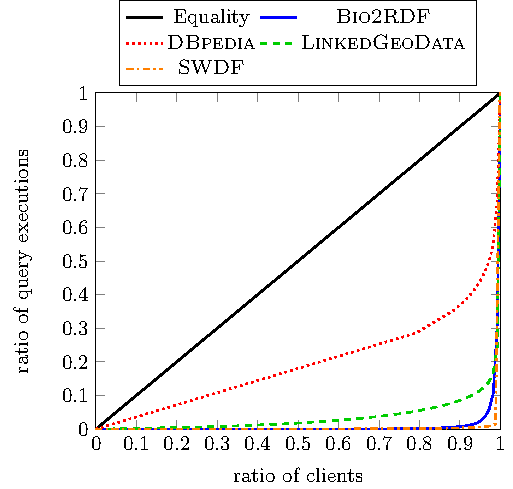
\includegraphics[width=\linewidth]{lorenz/client-lorenz-b2r}
\caption{Lorenz curve for distribution of executions per client}
\label{fig:client_lorenz}
\end{minipage}
\hfill
\begin{minipage}{0.49\textwidth}
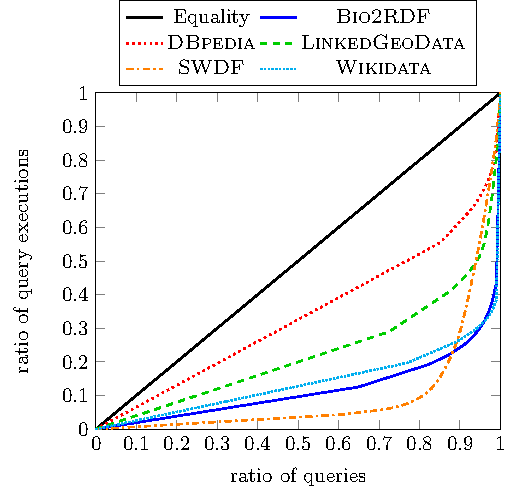
\includegraphics[width=\linewidth]{lorenz/query-lorenz-b2r}
\caption{Lorenz curve for distribution of executions per query}
\label{fig:query_lorenz}
\end{minipage}
\end{figure*}


\paragraph{Static and Runtime Statistics} Next, in order to characterise how complex the queries are to evaluate, in Table~\ref{tab:avgcomp} we present some relevant static and runtime statistics, where static statistics can be computed from the query string, while runtime statistics require evaluating the query locally (only queries that were successfully run are counted; see Table~\ref{tab:dsbstats} for statistics on runtime errors). Regarding runtimes, we recall that these were run with a one minute timeout, which represents the max runtime.
% TODO Complete statement below; it was just marked as blue and not as a todo note!
%{\color{blue}The minimum runtimes ...}
We see that \linkedgeodata contains the most costly queries to run, which appears to correlate with larger result sizes and a larger mean join-vertex degree. Relatively high runtimes are also seen for the \kegg dataset. The simplest queries to run are found in the \genage, \gendr and \taxonomy datasets. These results suggest, for example, that \linkedgeodata might be more suitable for consumers looking for a challenging benchmark.


\begin{table*}
\setlength{\tabcolsep}{1.4ex}
\centering
\caption{Comparison of the mean values of runtime statistics across all query logs (PVs = Project Variables, BGPs = Basic Graph Patterns, TPs = Triple Patterns, JVs = Join Vertices, MJVD = Mean Join Vertex Degree, MTPS = Mean Triple Pattern Selectivity)}
\label{tab:avgcomp}
\begin{tabular}{lrrrrrrrr} \toprule
\multirow{2}{*}{\textsc{Dataset}} & \multicolumn{5}{c}{\textsc{Static Statistics} (mean)} & \multicolumn{3}{c}{\textsc{Runtime Statistics}  (mean)} \\ 
 & PVs & BGPs & TPs & JVs & MJVD & MTPS & \textsc{Result Size} & \textsc{Runtime (sec)} \\ 
\cmidrule(r){1-1}\cmidrule(lr){2-6}\cmidrule(l){7-9}
\affymetrix & 1.93 & 1.06 & 1.10 & 0.03 & 0.06 & 0.82 & 12708.39 & 0.084\\
\biomodels & 1.24 & 1.04 & 1.42 & 0.37 & 0.75 & 0.57 & 4896.67 & 0.011\\
BIOPORTAL & 1.16 & 1.03 & 1.94 & 1.43 & 1.12 & 0.54 & 1699.48 & 0.004\\
\ctd & 2.56 & 1.05 & 1.08 & 0.02 & 0.04 & 0.85 & 24354.24 & 0.102\\
\dbpedia & 2.78 & 2.37 & 3.23 & 0.93 & 0.66 & 0.01 & 114038.38 & 0.164\\
\dbsnp & 1.09 & 1.02 & 1.04 & 0.02 & 0.04 & 0.97 & 757108.37 & 0.009\\
\drugbank & 2.61 & 1.05 & 1.93 & 0.69 & 0.91 & 0.66 & 119759.38 & 0.007\\
\genage & 1.88 & 1.00 & 1.09 & 0.04 & 0.13 & 0.99 & 1642.84 & 0.003\\
\gendr & 2.73 & 1.00 & 1.08 & 0.08 & 0.09 & 0.97 & 83.50 & 0.003\\
\go & 1.46 & 1.10 & 1.37 & 0.22 & 0.38 & 0.02 & 93806.20 & 0.046\\
\goa & 1.87 & 1.03 & 1.12 & 0.08 & 0.16 & 0.85 & 7692.26 & 0.016\\
\hgnc & 1.91 & 1.05 & 1.29 & 0.23 & 0.35 & 0.80 & 2419.43 & 0.019\\
\irefindex & 2.92 & 1.13 & 1.43 & 0.19 & 0.25 & 0.82 & 32200.76 & 0.077\\
\kegg & 2.27 & 1.15 & 1.31 & 0.13 & 0.18 & 0.33 & 175469.53 & 3.862\\
\linkedgeodata & 2.27 & 1.16 & 2.62 & 1.10 & 1.76 & 0.15 & 11055973.09 & 6.788\\
\linkedspl & 2.01 & 1.00 & 1.00 & 0.00 & 0.00 & 1.00 & 9503.41 & 0.014\\
\mgi & 2.04 & 1.04 & 1.11 & 0.05 & 0.06 & 0.84 & 2050.76 & 0.178\\
\ncbigene & 1.39 & 1.02 & 1.04 & 0.03 & 0.04 & 0.95 & 10731.33 & 0.021\\
\omim & 1.83 & 1.07 & 1.26 & 0.17 & 0.18 & 0.77 & 3505.54 & 0.020\\
\pharmgkb & 1.96 & 1.34 & 2.48 & 1.06 & 1.08 & 0.39 & 255.61 & 0.017\\
\sabiork & 2.96 & 1.05 & 1.06 & 0.01 & 0.02 & 0.88 & 1610.77 & 0.005\\
\sgd & 1.45 & 1.12 & 1.96 & 0.35 & 0.18 & 0.58 & 108951.60 & 0.058\\
\sider & 1.34 & 1.00 & 1.01 & 0.01 & 0.01 & 0.98 & 9703.86 & 0.010\\
\swdf & 4.04 & 3.37 & 3.97 & 0.45 & 0.92 & 0.03 & 37362.67 & 0.007\\
\taxonomy & 1.77 & 1.17 & 1.53 & 0.23 & 0.59 & 0.69 & 1928.75 & 0.004\\
\wikidata & 3.00 & 2.47 & 4.73 & 1.06 & 1.81 & 0.00 & 17817773.63 & 0.412\\
\wormbase & 1.56 & 1.25 & 2.05 & 0.65 & 0.87 & 0.98 & 9888.61 & 0.007\\
\midrule
Overall & 2.07 & 1.26 & 1.71 & 0.35 & 0.47 & 0.65 & 1126559.96 & 0.440\\
\bottomrule
\end{tabular}
\end{table*}

\paragraph{LSQ dataset statistics} The LSQ 2.0 dataset, describing 43.95 million executions of 11.56 million unique queries, contains 1.24~billion triples, split into 27 named graphs (one for each of the datasets listed).\footnote{We exclude some named graphs created by Virtuoso.}

\section{LSQ Adoption}
\label{sec:lsq_adoption}

In this section we present how LSQ has been adopted since its initial release with four logs in 2015. We organise this discussion following the motivational use cases we originally envisaged, as presented in Section~\ref{sec:usecase}.
Table~\ref{tab:logstats} provides an overview of the research works that have used LSQ, and the relevant use case(s) that they target. We now discuss these works in more detail; note that in the case of works that relate to multiple use cases, we will discuss them once in what we identify to be the ``primary'' related use case. We further discuss some works that have used the LSQ dataset for use cases beyond the six we had originally envisaged.

\begin{table*}
\centering
\setlength{\tabcolsep}{1.2ex}
\caption{Research works making use of the LSQ dataset since its initial release, ordered by year and then alphabetically by author name, with relevant use cases indicated (UC1: Custom Benchmarks; UC2: SPARQL Adoption; UC3: Caching; UC4: Usability; UC5: Optimisation; UC6: Meta-Querying)}
\label{tab:logstats}
\begin{tabular}{lcccccccc}
\hline
\textsc{Name} & \textsc{Year} & UC 1 & UC 2 & UC 3 & UC 4 & UC 5 & UC 6 & Other \\
\hline
Saleem et al.~\cite{SaleemMN15} & 2015 &	\checkmark  &  &  &  &   & &	\\
Arenas et al.~\cite{arenas2016reverse} & 2016 & \checkmark & & & \checkmark &  &  &  \\
Benedetti and Bergamaschi~\cite{benedetti2016model} & 2016 & & & & \checkmark &  & & \\
Georgala et al.~\cite{georgala2016efficient} & 2016 & &  &  &  &  & & \checkmark \\
Han et al.~\cite{han2016statistical} & 2016 & & \checkmark & & & \checkmark & & \\
Hernandez et al.~\cite{hernandez2016querying} & 2016 & \checkmark & & &  &  &   & \\
Knuth et al.~\cite{knuth2016scheduling} & 2016 & \checkmark &  & \checkmark &  &  &   & \\
Rico et al.~\cite{rico2016data} & 2016 & & & & & & \checkmark & \\
%Ngomo and Saleem \cite{ngomo2016federated} & 2016 & \checkmark & & &  &  & & \\
Schoenfisch and Stuckenschmidt~\cite{schoenfisch2016analyzing} & 2016 &  & \checkmark &  &  & \checkmark & & \\
Song et al.~\cite{song2016efficient} & 2016 & \checkmark &  &  &  & \checkmark & & \\


Bonifati et al.~\cite{BonifatiMT17} & 2017 & & \checkmark & & & \checkmark & & \\
Dellal et al.~\cite{dellal2017addressing} & 2017 &  & &  & \checkmark &  &  &  \\
Fokou et al.~\cite{FokouJHB17} & 2017 & & & & \checkmark & & \\
Stegemann and Ziegler~\cite{stegemann2017investigating} & 2017 &	\checkmark  & \checkmark &  & \checkmark & &  & \\
Thakkar et al.~\cite{thakkar2017trying} & 2017 & \checkmark &  &  &  &   &  &  \\

Akhtar et al.~\cite{akhtar2018change} & 2018 & \checkmark &  & \checkmark &  &  & & \\
Bonifati et al.~\cite{bonifati2018darql} & 2018 & & \checkmark &  &  & \checkmark & & \\
Darari et al.~\cite{darari2018completeness} & 2018 &  &  &  &  &   &  & \checkmark \\
Martens and Trautner~\cite{MartensT18} & 2018 & & & & & \checkmark & & \\
Salas and Hogan~\cite{SalasH18} & 2018 & \checkmark & & \checkmark  & & & & \\
Saleem et al.~\cite{saleem2018largerdfbench} & 2018 & \checkmark &  &  &  &   & &	\\
Saleem et al.~\cite{SaleemMSLN18} & 2018 & \checkmark &  &  &  &   & &	\\
Varga et al.~\cite{varga2018analytical} & 2018 & & & & & & \checkmark & \\
Viswanathan et al.~\cite{Viswanathan18} & 2018 & & & & \checkmark & & \\

Akhtar et al.~\cite{akhtar2019dynamic} & 2019 & \checkmark &  & \checkmark &  &  & & \\
Cheng and Hartig~\cite{cheng2019opt+} & 2019 & \checkmark & \checkmark &  &  & \checkmark & &	\\
Fafalios and Tzitzikas~\cite{fafalios2019many} & 2019 & &  &  &  &   & & \checkmark	 \\
Fernandez et al.~\cite{fernandez2019evaluating} & 2019 & \checkmark & & &  &  &   &  \\
Potoniec~\cite{Potoniec19} & 2019 & \checkmark & & & \checkmark & & & \\
Saleem et al.~\cite{SaleemSCBMN19} & 2019 & \checkmark &  &  &  &   & &	 \\
Thost and Dolby~\cite{thost2019qed} & 2019 & \checkmark &  &  &   &   & & \checkmark \\
Wang et al.~\cite{wang2019answering}  & 2019 & &  &  & \checkmark &  & & \\
Savafi et al.~\cite{safavi2019personalized}  & 2019 & & & \checkmark &  &  & & \\
Singh et al.~\cite{singh2019qaldgen}  & 2019 &\checkmark &  &  &  &  & & \checkmark \\
Azzam et al.~\cite{azzam2020smart}  & 2020 & \checkmark &  &  &  &  & & \\
Bigerl et al.~\cite{bigerl2020tentris}  & 2020 & \checkmark&  &  &  &  & & \\
Bonifati et al.~\cite{BonifatiMT20} & 2020 & & \checkmark & & \checkmark & \checkmark & & \\
Figueira et al.~\cite{FigueiraGKMNT20} & 2020 & & \checkmark & & &  \checkmark & & \\
Jian et al.~\cite{jian2020sparql}  & 2020 & \checkmark &  &  & \checkmark  &  & & \\
Zhang et al.~\cite{zhang2020revealing}  & 2020 & \checkmark & &  & \checkmark  &  & & \\

Aebeloe et al.~\cite{AebeloeMH21} & 2021 & \checkmark &  &  &  &  & & \checkmark \\
Almendros-Jimenez et al.~\cite{ALMENDROSJIMENEZ2021113772} & 2021 & \checkmark &   &  & \checkmark &  & & \\
Azzam et al.~\cite{AzzamAMKPH21}  & 2021 & \checkmark &  &  &  &  & & \\
Davoudian et al.~\cite{davoudian2021workload} & 2021 & \checkmark&   &  &  &  & & \\
Desouki et al.~\cite{9364498} & 2021 & \checkmark&   &  &  &  & & \\
Röder et al.~\cite{9364380}  & 2021 & \checkmark&   &  &  &  & & \\
Wang et al.~\cite{wang2021explaining} & 2021 & \checkmark&   &  & \checkmark &  & & \\
%Azzam et al.~\cite{AzzamAMKPH21}  & 2021 & \checkmark&   &  &  &  & & \\
\bottomrule
\end{tabular}
\end{table*}


\paragraph{UC1: Custom Benchmarks} LSQ has been adopted in various works for creating custom benchmarks. 

\begin{itemize}
\item Saleem et al.~\cite{SaleemMN15} present a framework for generating benchmarks that can be used to evaluate SPARQL endpoints under typical workloads; the benchmarks generate query types depending on the features of the queries submitted to the endpoint, where LSQ is used for testing. 
\item Later works by Saleem et al. further propose frameworks for generating benchmarks from LSQ for the purposes of evaluating query containment~\cite{SaleemMSLN18,saleem2017sqcframework} and federated query evaluation~\cite{saleem2018largerdfbench}, as well as comparing existing SPARQL benchmarks against LSQ in order to understand how representative they are of real workloads~\cite{SaleemSCBMN19}. 
\item Hern{\'a}ndez et al.~\cite{hernandez2016querying} present an empirical study of the efficiency of graph database engines for answering SPARQL queries over Wikidata; they refer to LSQ to verify that the query shapes considered for evaluation correspond with other analyses of real-world SPARQL queries. 
\item Fern{\'a}ndez et al.~\cite{fernandez2019evaluating} evaluate various archiving techniques and querying strategies for RDF archives that store historical data; in their evaluation, they select the 200 most frequent triple patterns from the \dbpedia query set in LSQ. 
\item Azzam et al.~\cite{azzam2020smart} use LSQ for retrieving highly-demanding queries from the dataset in order to evaluate their system for dividing the load processed by different SPARQL servers. 
\item Bigerl et al.~\cite{bigerl2020tentris} develop a tensor-based triple store, where they used LSQ as input to the FEASIBLE framework to generate a custom benchmark. 
\item Azzam et al.~\cite{AzzamAMKPH21} present a system that dynamically delegates query processing load between clients and servers. The authors use the Linked Data Fragments client/server approach improving it with the aforementioned technique and use 16 queries from LSQ to complement their evaluation.
\item Davoudian et al.~\cite{davoudian2021workload} present a system that partitions graphs depending on the access frequency to their nodes. In this way the system implements workload-aware partitioning. The authors use LSQ for evaluating their approach.
\item Desouki et al.~\cite{9364498} propose a method to generate synthetic benchmark data. To generate these synthetic data they use other RDF graphs available, such as \swdf and \dbpedia 2016. They benchmark their approach using queries from LSQ.
\item R\"oder et al.~\cite{9364380} develop a method to predict the performance of knowledge graph query engines; to do so the authors use a stochastic generation model that is able to generate graphs of arbitrary sizes similar to the input graph. They use LSQ as a benchmark of real-world queries.
\end{itemize}

%Saleem et al.~\cite{SaleemMN15,SaleemMSLN18} create a framework, called SQC-Framework, for generating benchmarks to evaluate \textit{query containment}---i.e., deciding if the result set of a given query is included in that of another given query---using the LSQ meta-data and clustering methods to select diverse real-world queries.

%Saleem et al.~\cite{SaleemMSLN18} create a framework, called SQC-Framework, for generating benchmarks to evaluate \textit{query containment}---i.e., deciding if the result set of a given query is included in that of another given query---using the LSQ meta-data and clustering methods to select diverse real-world queries.

%Saleem et al.~\cite{saleem2018largerdfbench} present a benchmark for federated SPARQL queries that span several distributed RDF datasets; to generate these queries the authors use LSQ.

%Ngonga Ngomo and Saleem~\cite{ngomo2016federated} present the challenges and opportunities in federated query processing, showing the need of using real SPARQL queries in the evaluation benchmarks, highlighting the use of LSQ to know which are the most popular queries a system should process most frequently. Aidan: I think this is covered by feasible.

% custom benchmark

%Saleem et al.~\cite{SaleemSCBMN19} provide an analysis of how to chose the most suitable benchmark for evaluating triple stores in practical settings, providing a a comparative analysis of existing SPARQL benchmarks with LSQ.

% custom benchmark


\paragraph{UC2: SPARQL Adoption}
\label{sec-sparql_adoption_uc}

Other works have used LSQ to understand how SPARQL is being used in practice. 


\begin{itemize}
\item Han et al.~\cite{han2016statistical} provide a statistical analysis of the queries of LSQ, surveying both syntactic features, such as the number of triple patterns, the SPARQL features used, the frequency of well-designed patterns; as well as semantic properties, such as montonicity, weak-monotonicity, non-monotonicity and satisfiability.
\item Bonifati et al.~\cite{BonifatiMT17,bonifati2018darql} conduct detailed analysis of the queries in various logs, including LSQ; they study a variety of phenomena in these queries, including their shape, their (hyper)treewidth, common abstract patterns found in the property paths, ``streaks'' that represent a sequence of user reformulations from a seed query, and more besides.
\end{itemize}   

\paragraph{UC3: Caching}
\label{sec-caching_uc}

LSQ can also be used to simulate real workloads for systems that explore caching techniques. 

\begin{itemize}
\item Knuth et al.~\cite{knuth2016scheduling} propose a middleware component to which applications register and get notifications when the results of their SPARQL queries change; the authors study the problem of scheduling refresh queries for a large number of registered queries and use LSQ to validate their approach. 
\item Akhtar et al.~\cite{akhtar2018change,akhtar2019dynamic} propose an approach to capture changes in an RDF dataset and update a cache system in front of the SPARQL endpoint exposing that data; their approach consists of a change metric that quantifies the changes in an RDF dataset, and a weighting function that assigns importance to recent changes; they use LSQ to verify their approach for real workloads. 
\item Salas and Hogan~\cite{SalasH18} propose a method for query canonicalisation, which consists in mapping congruous queries---i.e., queries that are equivalent modulo variable names---to the same query string; their main use case is to increase the hit rate of SPARQL caches, where they use LSQ to test efficiency on real-world queries and to see how many congruent queries can be found in real workloads.
\item Savafi et al.~\cite{safavi2019personalized} study SPARQL adoption using LSQ so they can later provide queries to summarise the Knowledge Graphs such that they can be more efficiently accessed from and stored on mobile devices with limited resources.
\end{itemize}

\paragraph{UC4: Usability}
\label{sec-usability_uc}

LSQ also has applications for improving the usability of SPARQL endpoints. 

\begin{itemize}
\item Arenas et al.~\cite{arenas2016reverse} propose a method for reverse-engineering SPARQL queries, which attempts to construct a query that will return a given set of positive examples as results, but not a second set of negative examples; the authors use LSQ to show that the approach scales well in the data size, number of examples, and in the size of the smallest query that fits the data. 
\item Benedetti and Bergamaschi~\cite{benedetti2016model} present a system (LODeX) that allows users to explore SPARQL endpoints more easily through a formal model defined over the endpoint schema; they show that LODeX is able to generate 77.6\% of the 5 million queries contained in the original LSQ dataset. 
\item Dellal et al.~\cite{dellal2017addressing} proposes query relaxation methods for queries with empty results, based on finding minimal failing subqueries (generating empty results) and maximal succeeding subqueries (generating non-empty results) to aid the user~\cite{FokouJHB17}. The paper refers to LSQ to establish that queries with empty results are common in practice.
\item Stegemann and Ziegler~\cite{stegemann2017investigating} propose new operators for the SPARQL language that allow for composing path queries more easily; the authors evaluated their approach with a user study and analysis of the extent to which their language is able to express the real-world queries found in LSQ.
\item Viswanathan et al.~\cite{Viswanathan18} propose a different form of query relaxation, which generalises a specific resource to a variable on which specific restrictions are added that correspond to relevant characteristics of the resource; they use LSQ to understand how entities are queried in practice. 
\item Potoniec~\cite{Potoniec19} proposes an interactive system for learning SPARQL queries from positive and negative examples;\footnote{Notably the system is called Learning SPARQL Queries (LSQ).} he uses the \dbpedia queries of LSQ for experiments. 
\item Wang et al.~\cite{wang2019answering} present an approach for explaining missing results for a SPARQL query---based on answering ``\textit{why-not}'' questions that ask why a specific result is not included---to help users refine their initial queries; the authors search LSQ for queries useful for their approach. 
\item Bonifati et al.~\cite{BonifatiMT20} analyse ``streaks'' in DBpedia query logs,\footnote{In fact, these logs were gathered directly from OpenLink, though we include discussion since similar analysis could have been applied to the LSQ logs, and LSQ logs where used in other analyses.} where a streak is defined as a sequence of similar queries in chronological order, capturing the idea of a user refining and/or extending an initial query towards a final query.
\item Jian et al.~\cite{jian2020sparql} use LSQ to evaluate their approach for SPARQL query relaxation (to generalise users' queries) and query restriction (to refine users' queries) based on approximation and heuristics.
\item Zhang et al.~\cite{zhang2020revealing} propose a method to model client behaviour when formulating SPARQL queries in order to predict their intent and optimise queries. They use LSQ for their evaluation.
\item Almendros-Jimenez et al.~\cite{ALMENDROSJIMENEZ2021113772} present two methods for discovering and diagnosing ``wrong'' SPARQL queries based on ontology reasoning. They evaluate their approach using LSQ queries.
\item Wang et al.~\cite{wang2021explaining} focus on providing explanations for SPARQL query similarity measures. The authors provide similarity scores using several explainable models based on Linear Regression, Support Vector Regression, Ridge Regression, and Random Forest Regression. They use LSQ to evaluate their query classification.
\end{itemize}

\paragraph{UC5: Optimisation}
\label{sec-optimisation_uc}

The LSQ dataset can also be used to identify and study fragments that are commonly used in practice and can be evaluated efficiently using dedicated algorithms. 
\begin{itemize}
\item The aforementioned analyses by Han et al.~\cite{han2016statistical} and Bonifati et al.~\cite{BonifatiMT17,bonifati2018darql} suggest that well-designed patterns, queries of bounded treewidth, etc., make for promising fragments. 
\item In the context of probabilistic Ontology-Based Data Access (OBDA), Schoenfisch and Stuckenschmidt~\cite{schoenfisch2016analyzing} analyse the ratio of safe queries---whose evaluation is tractable in data complexity---versus unsafe queries---whose evaluation is $\#$P-hard; they show that over 97.9\% of the LSQ queries are safe, and can be efficiently evaluated.
\item Song et al.~\cite{song2016efficient} use LSQ to analyse how nested \texttt{OPTIONAL} clauses affect query response times; they propose a way to approximate solutions for deeply-nested well-designed patterns.
\item Martens and Trautner~\cite{MartensT18} later take the property paths extracted by Bonifati et al.~\cite{BonifatiMT17} from LSQ and other sources, defining \textit{simple transitive expressions} that subsume almost all property path expressions seen in practice, while allowing more efficient evaluation than the general case. 
\item Cheng and Hartig~\cite{cheng2019opt+} introduce a monotonic version of the \texttt{OPTIONAL} operator to SPARQL called \texttt{OPT+}; a possible downside of the operator is an increase in query result sizes, where they use the LSQ dataset to study how \texttt{OPTIONAL} and \texttt{OPT+} behave for real-world queries.
\item Building upon the work of Martens and Trautner~\cite{MartensT18}, Figueira et al.~\cite{FigueiraGKMNT20} specifically study the containment problem for restricted classes of Conjunctive Regular Path Queries (CRPQs), which are akin to BGPs with property paths; aside from complexity results, they show the coverage of the different classes for logs that include LSQ~\cite{BonifatiMT20}.
\end{itemize}

%In~\cite{khouri2018lod} is just a reference in the state of the art.


\paragraph{UC6: Meta-Querying}
\label{sec-metaquerying_uc}

A handful of works have also used LSQ in the context of meta-querying, where queries are found based on the resources they contain. 

\begin{itemize}
\item Rico et al.~\cite{rico2016data} observe that analogous \dbpedia properties are often defined in two distinct namespaces---e.g., \texttt{dbo:birthPlace} and \texttt{dbp:birthPlace}---where they propose methods to automatically expand SPARQL queries to capture solutions involving analogous properties; they show that only 0.2\% of the \dbpedia queries in LSQ mention properties from both namespaces.
\item Varga et al.~\cite{varga2018analytical} provide an RDF-based metamodel for BI 2.0 systems, which allows for capturing the schema of a dataset, as well as previous queries that have been posed against that dataset by other users; the authors propose to re-use parts of the LSQ vocabulary in their model; they further instantiate their model using LSQ to retrieve queries asked about countries.
\end{itemize} 

\paragraph{Other use cases} A number of works have used LSQ (mostly for evaluation) in contexts that were not originally anticipated by the aforementioned use cases.

\begin{itemize}
\item Georgala et al.~\cite{georgala2016efficient} propose a method to predict temporal relations between events represented by RDF resources following Allen's interval algebra; they use LSQ to validate their approach considering query executions as events.  
\item Darari et al.~\cite{darari2018completeness} present a theoretical framework for augmenting RDF data sources with completeness statements, which allows for reasoning about the completeness of SPARQL query results; they evaluate their method using LSQ.
\item Fafalios and Tzitzikas~\cite{fafalios2019many} present a query evaluation strategy, called SPARQL-LD, that combines link traversal and query processing at SPARQL endpoints; they provide a method for checking if a SPARQL query can be answered through link traversal, and analyse a large corpus of real SPARQL query logs---including LSQ---for finding the frequency and distribution of answerable and non-answerable query patterns; they also use LSQ to evaluate their approach.
\item Singh et al.~\cite{singh2019qaldgen} use the LSQ vocabulary for providing a benchmark for Question Answering over Linked Data. The authors use the LSQ vocabulary to represent the SPARQL query related features prior to generating the benchmark. 
\item Thost and Dolby~\cite{thost2019qed} present QED: a system for generating concise RDF graphs that are sufficient to produce solutions from a given query, which can be used for benchmarking, for compliance testing, for training query-by-example models, etc.; they apply their system over LSQ queries to generate datasets from \dbpedia. 
\item Aebeloe et al.~\cite{AebeloeMH21} present a decentralised architecture based on blockchain that allows users to propose updates to faulty or outdated data, tracing back their origin, and query older versions of the data. They use LSQ queries for their evaluation. 
\end{itemize}

\paragraph{Discussion} Per Table~\ref{tab:logstats}, we see that the original version of LSQ has been used in a wide variety of research works for a variety of purposes. Complementing other SPARQL query logs such as Wikidata's~\cite{MalyshevKGGB18}, we believe that LSQ~2.0, with its extended set of queries, will likewise serve as a useful resource to help align the theory and practice of SPARQL research.

\section{Conclusions and Future Directions}
\label{sec:conclusion}

In this paper, we have described the Linked SPARQL Queries v.2 (LSQ~2.0) dataset, which represents queries in logs as RDF, allowing clients to quickly find real-world queries that may be of interest to them. We have described a number of use cases for LSQ, including the generation of custom benchmarks, the analysis of how SPARQL is used in practice, the evaluation of caching systems, the exploration of techniques to improve the usability of SPARQL services, the targeted optimisation of queries with characteristics commonly found in real workloads, as well as the ability to find queries relating to specific resources. We then described the model and vocabulary used to represent LSQ, including static features of queries, a SPIN representation, provenance encoding the agents and endpoints from which the query originate, as well as runtime statistics generated through local executions of the queries against their corresponding dataset. We then discussed how LSQ is published, thereafter describing the datasets and queries featured in the current version of LSQ. Finally we discussed how LSQ has been used for research purposes since its initial release in 2015.

As discussed in Section~\ref{sec:lsq_adoption}, since its initial release, LSQ has been adopted by a variety of research works for a variety of purposes. In terms of future directions, we will look to continue adding further logs with further queries to the dataset. Looking at how LSQ has been adopted in the literature has also revealed ways in which the metadata for LSQ could be extended in a future version, such as to add information about monotonicity and satisfiability~\cite{han2016statistical}, or information about (hyper)treewidth~\cite{BonifatiMT17,bonifati2018darql}, for example. It may also be useful to provide a canonical version of the query string~\cite{SalasH18}; this could perhaps be leveraged, for example, when evaluating caching methods. Another useful feature would be to add questions in natural language that verbalise each query, which could be used, for example, in order to create datasets for training and testing question answering systems, as well as enabling users to find relevant queries through keyword search; given the large number of queries in the dataset, an automated approach may be applicable~\cite{NgomoBULG13}.

As discussed by Martens and Trautner~\cite{MartensT19}, query logs allow to bridge the theory and practice of SPARQL. They serve an important role, ensuring that the research conducted by the community is guided by the requirements and trends that emerge in practice. We thus believe that LSQ~(2.0) will continue to serve an important role in SPARQL research in the coming years.




% Management

%
\section{Introduction}
\label{sec:introduction}
The vision of the Semantic Web is to establish a uniform machine readable infrastructure for data. Key technologies include: RDF\footnote{\url{https://www.w3.org/TR/rdf11-concepts/}} as a uniform data model to represent information about any domain, RDFS\footnote{\url{https://www.w3.org/TR/rdf11-schema/}} and OWL\footnote{\url{https://www.w3.org/TR/owl2-overview/}} for schema definition and reasoning, SHACL\footnote{\url{https://www.w3.org/TR/shacl/}} and ShEx\footnote{\url{http://shex.io/shex-semantics/}} for validation, and SPARQL\footnote{\url{https://www.w3.org/TR/sparql11-query/}} for querying.
%\footnote{The data model defines the overall structure of the data such as tabular, hierarchical or graph-based. The schema specifies a set of terms (such as attributes or types) that can be used within the model. The validation ensures that an instance of the data model satis}
Foundational RDF vocabularies include: VoID\footnote{\url{https://www.w3.org/TR/void/}} for statistical information about dataset content,
DCAT\footnote{\url{https://www.w3.org/TR/vocab-dcat-3/}} for decentral data (and service) catalogs, P-Plan\footnote{\url{http://purl.org/net/p-plan}} for describing execution plans, PROV-O\footnote{\url{https://www.w3.org/TR/prov-o/}} for provenance.

The FAIR principles~\cite{wilkinson2016fair} provide a conceptual framework for designing data publishing processes in a comprehensible way that makes the involved artifacts findable, accessible, interoperable and reusable.
%While the FAIR principles are a foundation for reproducible builds of data artifacts, the principles do not go as far as to demand that.
%In software engineering, the concept of reproducible builds---build specifications where independent executions in identically configured environments produce the exact same output bit-by-bit---is widely supported. As always, practical considerations may justify deviations.
As an example, while mapping non-RDF data with RML\footnote{\url{https://rml.io/specs/rml/}} (and variants such as YARRML\footnote{\url{https://rml.io/yarrrml/spec/}}) is common, the tracking of which input CSV artifact was converted by which RML mapping to which output RDF file is not.
One possible approach to address this problem is the Common Workflow Language (CWL)\cite{crusoe2022methods}.
One motivation for the creation of CWL is that by now there are dozens of workflow engines\footnote{\textls[-20]{\url{https://github.com/meirwah/awesome-workflow-engines/blob/master/README.md}}} and hundreds of data analysis pipeline systems\footnote{\url{https://s.apache.org/existing-workflow-systems}} with hardly any interoperability, so there is a strong need for a unifying language.
However, despite the availability of all these solutions for particular problems,
approaches for publishing data in an automated way not only according to the FAIR principles
but also in reproducible ways are still uncommon.
%the exception.

Apache Maven\footnote{\url{https://maven.apache.org/}} excels at the following aspects w.r.t. the management of artifacts: (1) findability of artifacts through repository managers, especially Maven Central\footnote{\url{https://central.sonatype.com}}, (2) easy accessibility of artifacts via plain HTTP(S) downloads, (3) interoperability on the repository level with various tools (such as Gradle, Ivy, SBT) and (4) reusability of artifacts via dependency management.
Further aspects are stable versioning of build outputs and the high extensibility of builds via plugins.
We identify a gap between data catalog systems and repository managers and with this work we propose a prototype architecture to bridge it.

Our contributions are as follows: (1) We perform an in-depth analysis for whether and how the Apache Maven build system can be adopted for several DataOps aspects and assess the technical feasibility.
% Rephrase: Wir machen eine Machbarkeitsstudie inwieweit sinch Maven für DataOps eignet
(2) As a resource, we set up a website \emph{Maven4Data}\footnote{\url{https://scaseco.github.io/maven4data}} which documents technical details and collects additional examples. (3) As software, we provide one Maven plugin for SPARQL and RML processing, and another for uploading artifacts to the Comprehensive Knowledge Archive Network (CKAN).
(4) We provide \emph{mvn-rdf-sync}\footnote{\url{https://github.com/Scaseco/mvn-rdf-sync}} as an additional software prototype. It is a Docker Compose setup for reacting to changes in a Maven repository in order to auto-generate DCAT metadata as well as publishing that DCAT in a triple store.
(5) A basic benchmark framework for assessing the performance impact of mvn-rdf-sync on a repository system is provided.

%Devising a data pipeline is foremost a design task. Implementations can range from custom bash scripts to graphically edited workflows on hosted platforms. Therefore Requirements are needed to guide this process.
%\begin{itemize}
%    \item Versioning of artifacts
%    \item Consistent naming of data artifacts
%    \item Locality: Data generation processes should. 
%    \item Open source ecosystem (and self-hosted).
%\end{itemize}
%- Nextcloud vs Archiva
%In this work we focus on semantic data integration using ETL .
%As a guiding example, we present two use cases
%- RDFization of GTFS data.
%- Consumption of disaster information from Web APIs.
%In this work, as a running example, our goal is to model a process a GTFS CSV file to RDF via RML and generate an Apache Jena TDB2 database file from it.
%\todo{It is important to note that build systems and workflow engines are complementary tooling. We focus on the aspects that Maven excels at.}
%- Semantic Data integration
%We identify gaps in~\autoref{sec:requirements}.
The remainder of this work is structured as follows.
In~\autoref{sec:related-work} we present related work for processing, packaging and FAIR publishing of data artifacts based on Semantic Web technology.
An introduction to the Maven build system is given in~\autoref{sec:maven}.
Applying the Maven system to RDF data management is elaborated in~\autoref{sec:data}.
Synchronization of DCAT metadata from a Maven repository with a triple store is presented in~\autoref{sec:mvn-sync}.
A brief performance evaluation for triggering metadata generation upon data deployment is presented in ~\autoref{sec:eval}.
Finally, we conclude this work in~\autoref{sec:conclusions}.

\section{Related Work}
\label{sec:related-work}

%\vspace{-2mm}
\paragraph{OntoMaven}\cite{paschke2018ontomaven} provides a set of Maven plugins for working specifically with ontologies (rather than RDF in general). Plugin goals exist to perform inferencing, testing, and the generation of HTML documentation with graph visualizations (somewhat similar to Javadoc). The focus of OntoMaven is to assist with agile ontology development process models such as RapidOWL\cite{auer2006rapidowl} and the Corporate Ontology Lifecycle Methodology (COLM)\cite{luczak2009managing}.

%\vspace{-2mm}
\paragraph{DBpedia Databus} is a data asset release
management platform inspired by paradigms and techniques successfully
applied in software release management\cite{DBLP:conf/mtsr/FreyGHH21}. The Databus project explicitly borrows concepts from Apache Maven and also features a set of maven plugins. However, the project features its own platform with its own APIs.
The crucial difference between the Databus project and this work is, that
here we investigate how data processing processes can be performed natively with Apache Maven and deployment idiomatically with the  (WebDav) API support by conventional artifact repository management systems. Plugins such as those of the Databus can be used in addition.

%\vspace{-2mm}
\paragraph{Common Workflow Language (CWL)} is an attempt to establish a common language for workflows. The reference implementation \emph{cwltool} also aims to leverage Semantic Web technology as a means for data generation adhering to the FAIR principles. %However, it does not consider versioning or publishing as part of its job.
Whereas versioning of artifacts is an intrinsic concept in Maven, the architecture around CWL relies on external services such as WorkflowHub\footnote{\url{https://workflowhub.eu/}}~\cite{goble2021implementing}.
Due to the relevance of CWL, we assembled a feature comparison with Maven in~\autoref{tab:mvn-vs-cwl} in order to provide more insights into their similarities and differences.
%\vskip\baselineskip
%assembled a detailed feature comparison between Maven and CWL

%\vspace{-2mm}
\paragraph{Research Object Crates} (RO-Crate)\cite{soiland2022packaging}\footnote{\url{https://www.researchobject.org/}} is a specification for annotating the content of a directory (or archive) with semantic descriptions. It seems feasible that such descriptions could be generated as part of a Maven build.

\vspace{2mm}In~\cite{hauptmann2015scalable}, a system for data version control on the RDF graph level is discussed.
This is an implementation that works only on the triple level of RDF data and has no regard to sources or transformations.

%One of the example workflows presented in this paper makes use of the RdfProcessingToolkit's  RML Toolkit\cite{stadler2023-scaling-rml} (rmltk) for executing RML mappings. It would also be possible to program this step using another tool, such as the RMLMapper\cite{dimou2014rml}.

%\todo{Add citations: RMLMapper, rmltk citations. Also Jena.}

%The authors of~\cite{bhardwaj2014datahub} suggest a centralised platform to store multiple versions of datasets for archival and download, together  with a specific SQL query language extension to take versions into account.

\paragraph{Data Version Control}\footnote{\url{https://dvc.org}} is a system/suggestion to use a Git-like approach and decentralised repositories to control different versions of personal datasets. Using their registry requires a commercial subscription.

\vspace{2mm}The Semantic Web components of our suggested approach are implemented using the Apache Jena\footnote{\url{https://jena.apache.org}} Semantic Web framework.

\begin{table}[p!]
\centering
\bgroup
\renewcommand{\arraystretch}{1.5}
\setlength{\tabcolsep}{0.5em}
%\begin{footnotesize}
\begin{tabular}{p{2.5cm}|p{4.5cm}|p{4.5cm}}
\toprule
\textbf{Feature} & \textbf{CWL} & \textbf{Maven} \\
\midrule
Versioning build outputs
&
CWL itself does not manage versioning of build outputs.
& 
Intrinsic support, using its coordinate system (groupId, artifactId, version).
\\

Versioning workflow plans
&
No intrinsic versioning system. Relies on external version control systems like Git.
&
Versioning is intrinsic to the POM file, allowing versioning of the project definition itself alongside the codebase.
\\

Dependency management
&
CWL specifies dependencies in terms of software containers and scripts required to run a workflow but relies on external tools for managing these dependencies.
&
Declaration and automatic downloading (and caching) of dependencies from central and custom repositories.
\\

Deployment of build outputs
&
No instrinic support. Requires scripting or external tools.
&
Built-in support for deploying artifacts to repositories through its deployment lifecycle phases and plugins.
\\

Containerization support (Docker)
&
Natively support for defining steps to be executed in Docker containers, making it straightforward to ensure environment consistency across executions.
&
Support via plugins but not as seamlessly integrated as CWL's native support.
\\

Signing build output
&
CWL does not have built-in support for signing outputs.
Any signing would need to be handled by external tools or steps defined within the workflow.
&
Maven supports signing artifacts via plugins (e.g., GPG Plugin) as part of its build process, ensuring the integrity and origin of build outputs.
\\

Deployment to alternative repositories
&
Deployment to alternative repositories would require integration with other tools.
&
Highly extensible, with a wide range of plugins available for deploying to various types of repositories.
\\

Execution model
&
DAG-based
&
Linear (Life-cycle based). Phases are executed in order - parallelism possible within phases.
\\

Execution monitoring
&
In addition to logging, third-party tools or workflow engines that support CWL can provide insights into each step's execution status and resource usage. Live-graph visualization possible such as using Apache Airflow.
&
Due to the linear processing nature typically only console logging and reporting.
\\

\bottomrule

\end{tabular}
%\end{footnotesize}
\egroup
\caption{Comparison between CWL and Maven}
\label{tab:mvn-vs-cwl}
\end{table}


\section{Introduction to Apache Maven}
\label{sec:maven}
Although Maven\footnote{\url{https://maven.apache.org/}} is a build tool mainly used for Java development, its underlying concepts are more general in nature.

% \subsection{A Model (not only) for Software Projects}
Maven is based on the concept of a project object model (POM).
The POM is the fundamental configuration file that contains information about the project, tasks, and dependencies.
Maven uses this file to do everything that is needed to build a project.
Applied to data management, this POM can be used to describe how to download, convert, and process data as well as the software and data dependencies required for a specific dataset.
The POM also contains several metadata fields that can be used to further link the project to source code repositories, applicable license information, author information and so on, which can be easily mapped to RDF.
Maven has built-in support for properties, together with substitution of placeholders in strings (aka interpolation) and files (aka resource filtering). This mechanism can be exploited for generating RDF with additional metadata.
Furthermore, Maven is capable of publishing the processed and generated data as artifacts to repository systems, and to download existing artifacts from there. % from them. %remote repositories.
%The processes that Maven calls upon when working with data and software codes can be extended using
Maven build workflows are based on invoking Maven plugins. Maven plugins are written in the Java programming language and can be deployed as artifacts to such repositories.
For a Java software project, Maven would typically call the \texttt{maven-compiler-plugin} to process the source code.

% disabled for now, I think it is not so relevant to your main content (by sbin)
% Maven introduces the notion of \emph{life cycles} for carrying out tasks on a software project in a certain order.
% %Builds for different project types are organized as \emph{life cycles.}
% A life cycle has a name and defines a sequence of \emph{phases}. 
% The actual functionality is provided by plugins. A plugin is essentially a JAR bundle with metadata about which \emph{goals} it provides. Goals are the actual methods that can be \emph{executed} on a plugin.
% % Explain bind - its establishing the relation between a phase and a goal
% The declaration about which plugin goal to execute in which phase is called \emph{binding} and can be carried out in different ways:
% \begin{itemize}
%   \item The life cycle specification can declare defaults about which plugins to execute in which of its phases.
%   \item A plugin can declare a phase it binds to by default
%   \item The developer can manually bind a plugin to a phase.
% \end{itemize}

% disabled for space reasons
% \begin{figure}
%   \centering
%   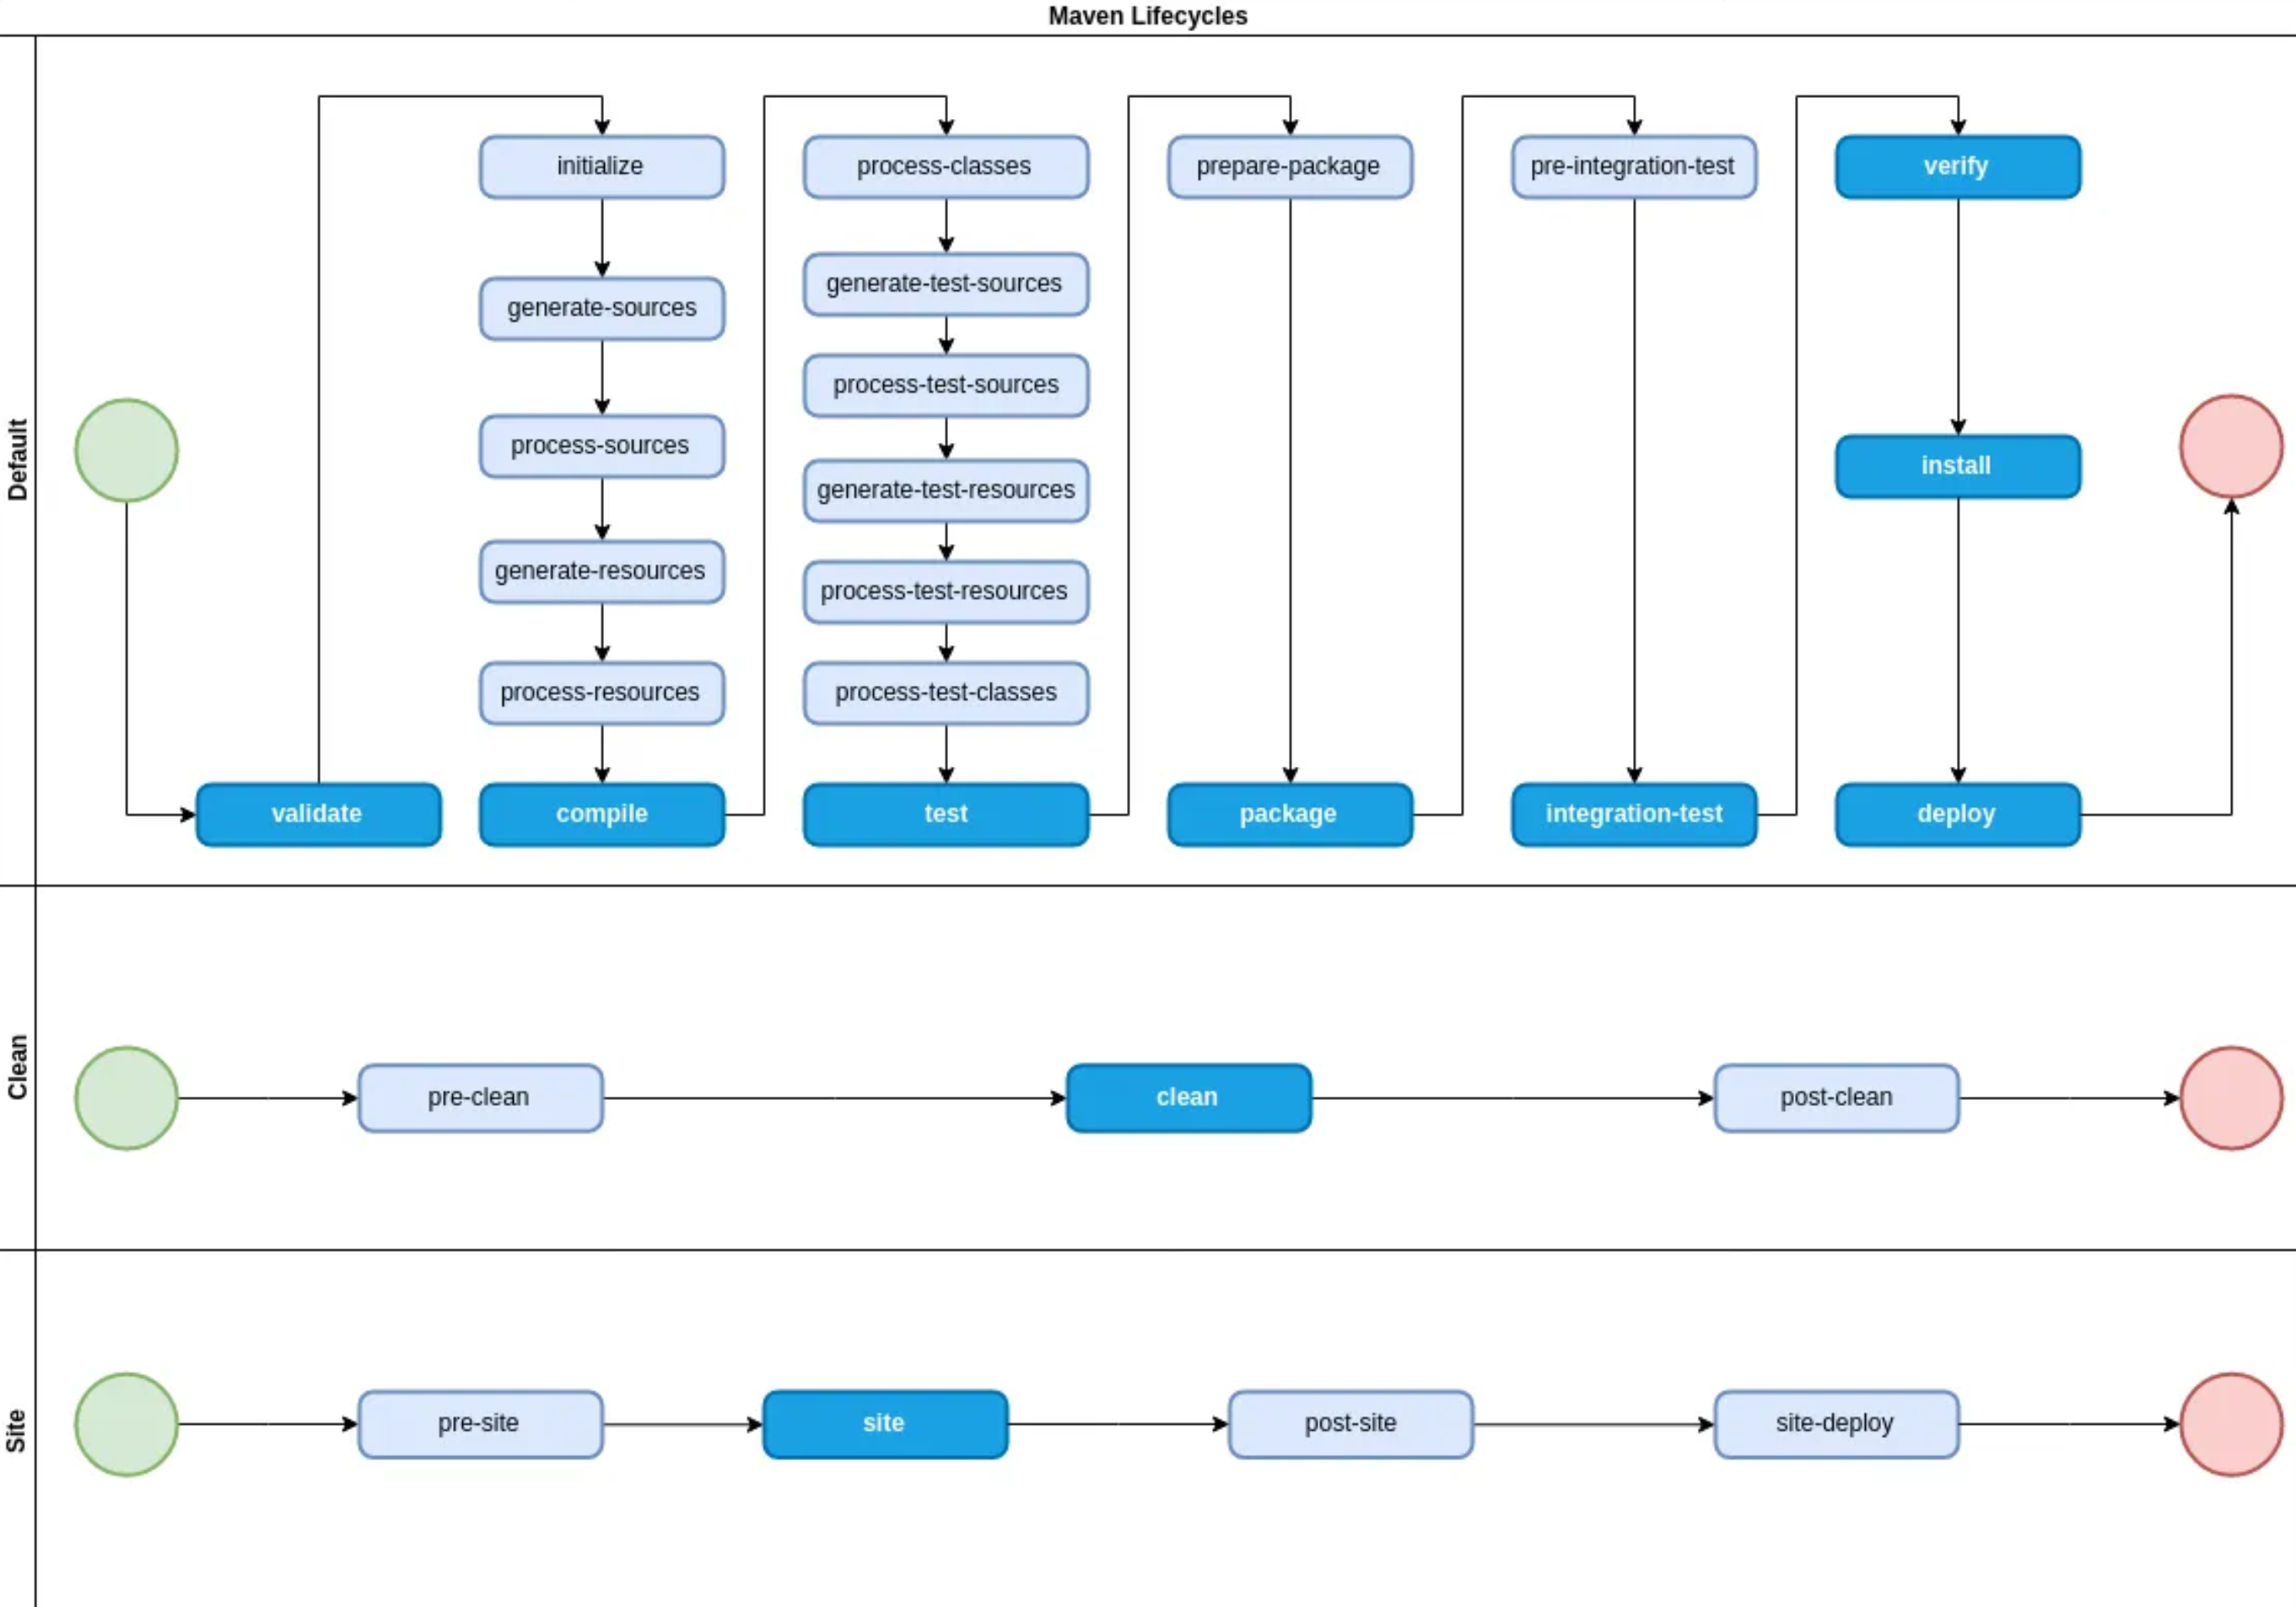
\includegraphics[width=0.8\textwidth]{images/maven-lifecycles.png}
%   \caption{Standard Maven Lifecycles and their goals.} 
%   \footnote{\footnotesize{\url{https://medium.com/@yetanothersoftwareengineer/maven-lifecycle-phases-plugins-and-goals-25d8e33fa22}}}
% \end{figure}

%The key message is, that Maven's view of a software project includes several phases, from generating sources, resources, over compilation to executing tests, caching the result locally and deploying to remote targets.

Maven introduces the notion of life cycles for carrying out tasks on a software project in a certain order.
A life cycle has a name and defines a sequence of phases. 
The phases \texttt{generate-resources} and \texttt{process-resources} are specifically dedicated to generating and packaging resources -- such as data.
The POM follows a single inheritance model such that common configuration options can be placed into a ``parent'' POM.
A typical use case for a parent POM is to configure the repositories to use for dependency resolution and artifact deployment as well as which versions of certain plugins to use.
% \subsection{POM Syntaxes}
Traditionally, POM files are written in XML and tool-chains typically operate on the XML model.
However, nowadays is also possible to write POMs in other popular languages (such as YAML) using the \texttt{polyglot-translate-plugin}\footnote{\url{https://github.com/takari/polyglot-maven}}.

% disabled, focus on the key aspects (by sbin)
% Maven polyglot is the response to the decline in XML's popularity.
% Polyglot is a project that enables the specification of the the project model in many alternative syntaxes, including JSON, YAML or Ruby. \autoref{fig:maven-polyglot} shows how to enable it. During build, each syntax is then converted to the usual pom.xml file.
% Existing pom files can be converted to alternative syntaxes using the following invocation:

% disabled for space reasons
% %\begin{figure}
% \begin{footnotesize}
% \begin{minted}{bash}
% mvn io.takari.polyglot:polyglot-translate-plugin:translate \
%   -Dinput=pom.xml -Doutput=pom.yml
% \end{minted}
% \end{footnotesize}
% %\end{figure}

% \begin{figure}
% \begin{minted}{xml}
% <?xml version="1.0" encoding="UTF-8"?>
% <extensions>
%     <extension>
%         <groupId>io.takari.polyglot</groupId>
%         <artifactId>polyglot-yaml</artifactId>
%         <version>0.7.0</version>
%     </extension>
% </extensions>
% \end{minted}
% \caption{This snippet in \texttt{.mvn/extensions.xml} enables support for \texttt{pom.yml}}
% \label{fig:maven-polyglot}
% \end{figure}

% \subsection{A Model for naming Artifacts}
%In this section we describe Maven's model for naming artifacts.
% Artifacts in Maven are located along a 5 dimensional coordinate system:
Each Maven project is described by a \emph{groupId}, an \emph{artifactId} and a \emph{version} (GAV). 
% Todo check manual newline position
The groupId is typically a reverse domain name such as \texttt{org.myorganiza\newline tion.mydepartment.myproject} and can thus be used to link an artifact to an organization in a Web-compatible way.
By using domains that are under ones own control, unique global identifiers that are nevertheless human-readable are ensured.
Artifact naming can also be leveraged for access control: For example, when publishing artifacts to Maven Central, permission is only granted to upload artifacts whose groupIds start with a specific prefix such as \texttt{org.myorgan\newline ization}.
Maven repositories can be configured to enforce that each version is only published exactly once, thereby ensuring that the exact state of a published dataset is not changed.
%(such as the Maven Central)

To each project GAV, any number of files can be attached. Files are differentiated by the type, such as jar, zip, ttl or nt.bz2, and a classifier, which can be any custom value. For example, in this work we use the classifier \emph{dcat} to tag the RDF metadata datasets to load into the triple store. One way to see a GAV is as a URN for a folder (or archive) which contains files with different names and types.
%\todo{@claus was macht man wenn man mehrere rdf dateien anhängen will?}
% Na halt andere classifier nehmen
Publishing a Maven project usually also attaches the POM file itself. POMs can be designed in a self-contained way such that the creation of artifacts becomes reproducible from the POM itself.

As for repository systems, Maven by default resolves dependencies against the central repository. The plugins we developed as part of this work are published there and can thus be readily reused in Maven builds. In order to not misuse the central repository as a data dump, we set up our own organization-wide repository system instance.
%While datasets can be deployed to the central repository it seems preferably to only do so in conjunction with software that relies on them (such as NLP tools).

% disabled because too long (by sbin)
% The three most fundamental fields are:
% \begin{itemize}
% \item The groupId is typically a domain name such as org.myorganization.mydepartment.myproject and can thus be used to link an artifact to an organization in a Web-compatible way.
% \item The artifactId is used as the name of a relevent unit of work within the group.
% \item The version naturally is an identifier to capture a "snapshot" of that unit of work a certain point in time.
% \end{itemize}
% These fields are often also referred to as the \emph{GAV}. A GAV can be seen as a name for a project, but additional fields are provided to \emph{attach} files to it:
% \begin{itemize}
% \item type: The type of the artifact. Usually a filename extension such as jar, zip or nt.bz2. As a Java-centric convention, if the type is left empty then it defaults to jar. So there is no "empty" type. The pom file itself has type "pom".
% \item classifier: A custom string to discriminate further files published under the same GAV, i.e. a tag. For example, in this work we use the classifier \emph{dcat} to tag the RDF datasets which to load into the triple store.
% \end{itemize}

% \subsubsection{Artifact Syntax}
% Maven coordinates are often represented with the syntax:
% % Some components use a different component order for use cases such as conflict resolution where the version comes last
% \texttt{groupId:artifactId:version[:type[:classifier]]}

% The [] indicate optional fields, so type and classifier may be omitted, but if a classifier is needed, then a type must be given as well.
% Obviously colons (:) must not be used within values for any of the fields.

% %See Maven's Guide to naming conventions for details about how to choose proper values and the valid characters.
% \subsubsection{Maven Coordinates, URNs, Files and Relative URLs}

% disabled due to length (by sbin)
% A maven coordinate can be effectively seen as an URN. We use the prefix \texttt{urn:mvn:} to represent maven coordinates as RDF IRIs.
% Maven coordinates can be unambiguously mapped to HTTP download links.
% The concept of separating naming and resolution of things with URNs is not new. Notably, Life Science Identifiers\footnote{\url{https://www.lsid.info/}} follow a similar pattern.
% %The difference is, that maven artifact resolution is simply HTTP(s)-based:
% Such Maven URNs can thus be converted to relative paths and prefixed with a repository's base URL in order to obtain a download URL.

%
%
% technische details, unwichtig (by sbin)
%  directory names and file names.
% These in turn correspond to relative URLs:
%     The groupId is turned into a directory prefix by replacing all . with /:
%     A filename is derived as follows:
%         If the classifier is absent, then the pattern is artifactId-[version].[type].
%         Otherwise it is, artifactId-[version]-[classifier].[type]
%
% Example without classifier. Lets assume a monthly report is published as a PDF file.
%
%     Coordinate: org.example:report:2024.02.01:pdf:
%     Translates to: org/example/report-2024.02.01.pdf
%
% Example with classifier. Let's assume a monthly report includes multiple files for different aspects such as sales.
%
%     Coordinate: org.example:report:2024.02.01:pptx:sales:
%     Translates to: org/example/report-2024.02.01-sales.pptx
%

%the final candidate URL for resolution.

% disabled because of length (by sbin)
% \subsubsection{Maven Artifact Repository Management Systems}
% Repository managers have emerged as a response to the need for central management of an organization's assets across several programming languages and tools.
% A repository manager provides control over the creation and access over repositories such as for debian, rpm, nodejs, java, ruby packages.
% \autoref{tab:storage} shows how artifact managers store maven artifacts. \emph{Files} means that maven WebDav uploads are directly mapped to physical files and folders on the file system, similar to maven's local repository.
% \emph{Blob} is and \emph{Hash} are storage abstractions. The former is Nexus's binary large object storage, whereas hash means that content is stored in files named according to a hash code of the content, whereas the mapping to paths is kept in a database.

% Artifact naming can be leveraged for access control: For example, when publishing artifacts to maven central\footnote{\url{https://central.sonatype.com/}}, permission is only granted to upload artifacts whose groupIds start with a specific prefix such as \emph{org.example}.
% %GroupId mimicks a domain name

% From a FAIR perspective, file storage has the advantage that it is easy to use. Any web server can publish a folders as static resources, incremental backups can be easily created using tools such as rsnapshot, and repository changes can be tracked with file system watches.



%\section{RDFization of Maven Repository Content}
\section{Adapting Maven for Data Generation and Deployment}
\label{sec:data}
In this section, we present a concrete selection of relevant tasks related to dataset management, representative of similar ones.
% The examples are on the maven4data website
We then provide a brief overview of the Maven plugins used to solve them.

\begin{figure}[!htb]
\centering
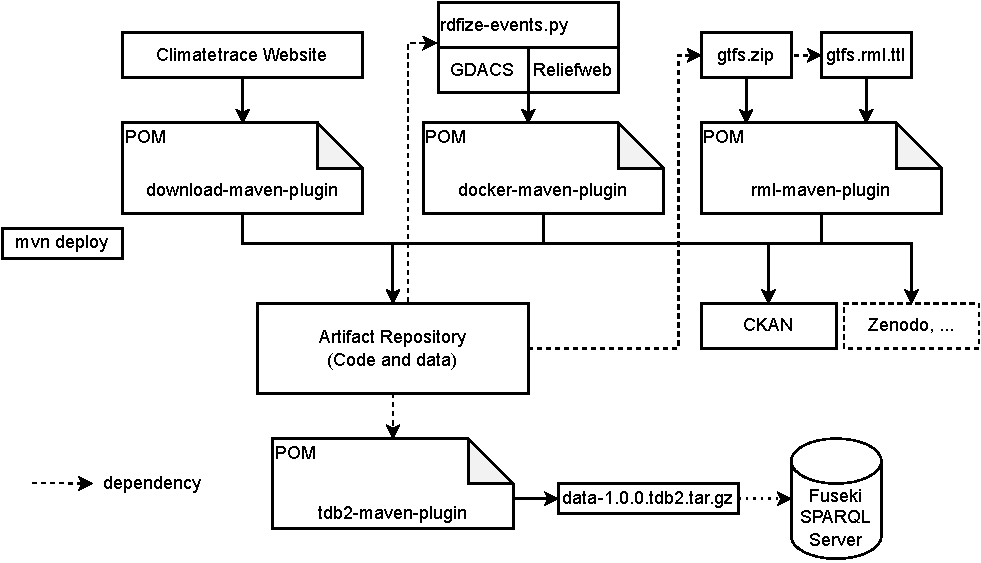
\includegraphics[width=0.8\textwidth]{images/mvn-data-architecture.pdf}
\caption{Architecture with different POM files for unified data processing.}
\label{fig:mvn-arch}
\end{figure}

\autoref{fig:mvn-arch} shows different setups with POM files that make use of different Maven plugins for the creation of artifacts by means of (a) downloading from the Climatetrace\footnote{\url{https://climatetrace.org/data}} website, (b) dockerized execution of a Python script that creates RDF based on data from the GDACS\footnote{\url{https://www.gdacs.org/}} and ReliefWeb\footnote{\url{https://reliefweb.int/}} Web services, and (c) RML mapping execution based on data and mapping files present in the artifact repository. 
Each POM can be executed with \texttt{mvn deploy} which produces the artifacts and uploads them both to a conventional Maven repository as well as to a CKAN instance. Additional plugins could be created for uploading artifacts also to e.g. Zenodo\footnote{\url{https://zenodo.org/}} or Huggingface\footnote{\url{https://huggingface.co/}}.
Furthermore, the \texttt{tdb2-maven-plugin}\footnote{\url{https://github.com/Scaseco/tdb2-maven-plugin}} is capable of creating a TDB2 database file that can be served using a Fuseki SPARQL server.

%\paragraph{Archiving downloads}. The task is to create a maven project whose build result is the downloading a given set of URLs and attaching them as files.
%This effectively enables republishing the content of URLs as maven URNs. This can be realised using the download-maven-plugin\footnote{\url{https://github.com/maven-download-plugin/maven-%download-plugin}}.\todo{Probably artifact download can be removed as its not our work anyway.}

% disabled (by sbin)
% \begin{minted}{yaml}
% build:
%   plugins:
%   - groupId: com.googlecode.maven-download-plugin
%     artifactId: download-maven-plugin
%     configuration: {url: '${input.url}', unpack: false,
%       outputDirectory: '${project.build.directory}',
%       outputFileName: '${output.filename}', skipCache: true}
%     executions:
%     - goals: [wget]
%       phase: process-resources
% \end{minted}

%There are several ways for how this 
%(a) Create one POM per file.
%(b) Attach all files to a single POM.
%(c) Package all downloads into a single archive (e.g. tar) and only attach the tar.

%\paragraph{Attaching files to a maven project}
%\paragraph{Marking files for inclusion in a project distribution}
\subsection*{Marking Files for Inclusion in a Project Distribution}
Files need to be \emph{attached} to a Maven project in order for them to be part of the file set that gets installed locally or deployed remotely.
Many plugins that generate files, such as the Javadoc one, directly support controlling whether to attach the generated files.
The \texttt{build-helper-maven-plugin} is the conventional way for attaching arbitrary files to a maven project using the \texttt{attach-artifact} goal. The GAV is predetermined by the POM, so attached files can only differ in their classifier and type values.
%\todo{(How) to attach generated data? What is supported by your own plugins? @claus (by sbin). The example showed that one just has to list the artifacts under the artifacts key....}

% disabled (by sbin)
% \begin{minted}{yaml}
% build:
%   plugins:
%   - groupId: org.codehaus.mojo
%     artifactId: build-helper-maven-plugin
%     executions:
%     - configuration:
%         artifacts:
%         - {file: '${project.build.directory}/${output.filename}',
%            type: '${output.filetype}'}
%       goals: [attach-artifact]
%       id: attach-artifacts
%       phase: package
% \end{minted}

%\paragraph{Using dockerized data generation}
\subsection*{Docker-based Data Generation}
The \texttt{docker-maven-plugin}\footnote{\url{https://dmp.fabric8.io/}} enables the use of Docker containers from within Maven builds. It supports copying files in and out of containers and requires a running Docker daemon.
For a complete example that runs a Python script to fetch information about disaster events and output them as RDF we refer to our supplemental web page\footnote{\textls[-34]{\url{https://scaseco.github.io/maven4data/how-tos/build-anything-with-docker.html}}}.

%\paragraph{RML Conversion}
\subsection*{RML Conversion}
In~\cite{stadler2023-kgcw-challenge} we presented a system based on our RML Toolkit~\cite{stadler2023-scaling-rml} (rmltk) that rewrites RML mappings to a sequence of extended SPARQL queries.
Likewise, we wrapped this system as a Maven plugin.
To use the system, two dependencies have been specified in the POM: one to an artifact containing the CSV source data, and one containing the RML mapping rules.
Then, the \texttt{rml-maven-plugin} is specified in the plugin section, together with an rmltk-specific configuration (also detailed inside the POM).
When Maven is called with process-resources, the dependencies and the plugins will be downloaded (unless they are already cached) and the mapping will execute.
A complete example is available on GitHub\footnote{\url{https://github.com/Scaseco/resource-gtfs-bench-rml/}}.

% disabled (by sbin)
% \begin{minted}{yaml}
% dependencies:
% - {groupId: org.aksw.data.gtfsbench, artifactId: gtfsbench-csv-1, version: 0.0.1-SNAPSHOT,
%   type: zip}
% - {groupId: org.aksw.data.gtfsbench, artifactId: mapping, version: 0.0.1-SNAPSHOT,
%   type: rml.ttl}
% build:
%   plugins:
%   # Omitted for brevity: Copying of dependencies to ${data.workdir}
%   - groupId: org.aksw.maven.plugins
%     artifactId: rml-maven-plugin
%     version: 0.9.0
%     executions:
%     - configuration:
%         outputFile: ${output.path}
%         outputFormat: ${output.filetype}
%         workDirectory: ${data.workdir}
%         mappings:
%         - {type: file, value: '${data.workdir}/mapping.rml.ttl'}
%       goals: [rml]
%       phase: process-resources
% \end{minted}

%\paragraph{RDF generation with SPARQL Queries}
\subsection*{RDF generation with SPARQL Queries}
We also created the \texttt{sparql-maven-plugin} to enable running SPARQL statements against an embedded triple store.
This enables loading of datasets as well as producing RDF with SPARQL CONSTRUCT queries as part of the build process.
The configuration is similar to that of the \texttt{rml-maven-plugin}
%\todo{@claus rpt plugin? or rml plugin?}
except that SPARQL queries can be provided as string and files.
This plugin can be used to produce VoID, DCAT and PROV metadata.
A crucial aspect is that Maven coordinate URNs of the POM can be used as the dataset identifier.

%\paragraph{Deploying to CKAN}
\subsection*{Deploying to CKAN}
CKAN\footnote{\url{https://ckan.org/}} is a popular open-source open data portal software for the storage and distribution of data. It has an API for uploading data and metadata.
We created the \texttt{ckan-maven-plugin} which enables uploading files to CKAN.
Several fields for the POM are directly mapped to fields in CKAN, such as: name, description and license. The plugin can be used in addition to any other plugins that carry out deployments.
Typically, all deployments are executed in the \texttt{deploy} phase. In general, a Maven build can be designed such that properties and profiles are provided to control which (sub)sets of plugins to execute. These mechanisms can be leveraged to carry out only specific deployments.
%
% disabled (by sbin)
% \begin{minted}{yaml}
% build:
%   plugins:
%     - groupId: org.aksw.maven.plugins
%       artifactId: ckan-maven-plugin
%       version: ${ckan-maven-plugin.version}
%       executions:
%         - id: ckan-upload
%           phase: deploy
%           goals: [upload]
%           configuration:
%             ckanUrl: https://your.ckan.instance/
%             serverId: your.ckan.serverId
%             datasetId: My Dataset Label
%             resourceId: ${project.artifactId}
%             fileName: ${output.path}
%             organizationId: my-ckan-org
%             author: Your Name
% \end{minted}
%
%Credentials for CKAN access are stored in the \texttt{\$HOME/.m2/settings.xml} file, as is customary for all credentials used by maven connectors.
The plugin supports reading (possibly encrypted) CKAN API keys from Maven's \texttt{settings.xml} file, which is Maven's default place for user-level passwords.
Note, that whether and how conventional dependencies can be (reasonably) resolved against a CKAN instance is future work.
%Note, that there is no established mapping procedure from Maven coordinates to CKAN entries, and 
More details about the configuration of the CKAN plugin is available on GitHub\footnote{\url{https://github.com/Scaseco/ckan-maven-plugin}}.
%\begin{minted}
%<server>
%  <id>your.ckan.serverId</id>
%  <username>your_username</username>
%  <password>your-optionally-encrypted-ckan-api-key</password>
%</server>
%\end{minted}


%\paragraph{Loading a triple store from dependencies}
\subsection*{Loading a Triple Store from Dependencies}
% disabled (by sbin)
% \begin{figure}
% \begin{footnotesize}
% \begin{minted}{yaml}
% modelVersion: 4.0.0
% parent: {artifactId: aksw-data-deployment, groupId: org.aksw.data.config,
%          version: 0.0.8, relativePath: ''}
% groupId: org.aksw.maven4data.examples
% artifactId: my-example-kg
% version: 1.0.0
% packaging: pom
% properties:
%   baseDir: ${project.build.directory} # Declaration for CWL interoperability!

% dependencies:
% - { groupId: org.coypu.data.disasters, artifactId: disasters,
%     version: 0.20240312.1842, type: nt.bz2 }
% - { groupId: org.aksw.moin, artifactId: moin,
%     version: 1.20220502.0, type: ttl.bz2 }
% build:
%   plugins:
%   - { groupId: org.aksw.maven.plugins, artifactId: tdb2-maven-plugin,
%       version: 0.0.1-SNAPSHOT }
%     executions:
%     - goals: [load]
% \end{minted}
% \end{footnotesize}
% \caption{pom.yml file for the creation of a TDB2 database archive.}
% \label{fig:tdb2-yml}
% \end{figure}
% %\end{minipage}

%\autoref{tdb2-yml} demonstrates the generation of a \emph{tdb2.tar.gz} for the provided RDF dependencies.\todo{get rid of snapshot}
We have created the \texttt{tdb2-maven-plugin}, that uses Apache Jena to convert RDF data into a TDB2 database suitable for use with Apache Jena.
%can be placed into a profile in order to not create the database archive by default. This way, \texttt{mvn deploy} will only deploy the \texttt{pom.xml} file without the data. This saves space in the archive and yet allows re-creation of the database any time in the future, such as when the need arises to perform evaluation on historic data.
To use it, the RDF datasets are specified as dependencies in the Maven POM, and the tdb2-maven-plugin is referenced in the build plugins section.
A limitation is, that Maven does not natively support the automatic build of missing artifacts based on a reference to a POM that could build those.
It may be possible to create further plugins that carry out such tasks by analyzing the dependency tree but but this is open to future work.

%of the database when using such a Maven project as a dependency in another project.
%client-side recreation of artifacts when referencing such a pom as a dependency.


\section{Synchronization of Metadata}
\label{sec:mvn-sync}
\begin{figure}[!htb]
\centering
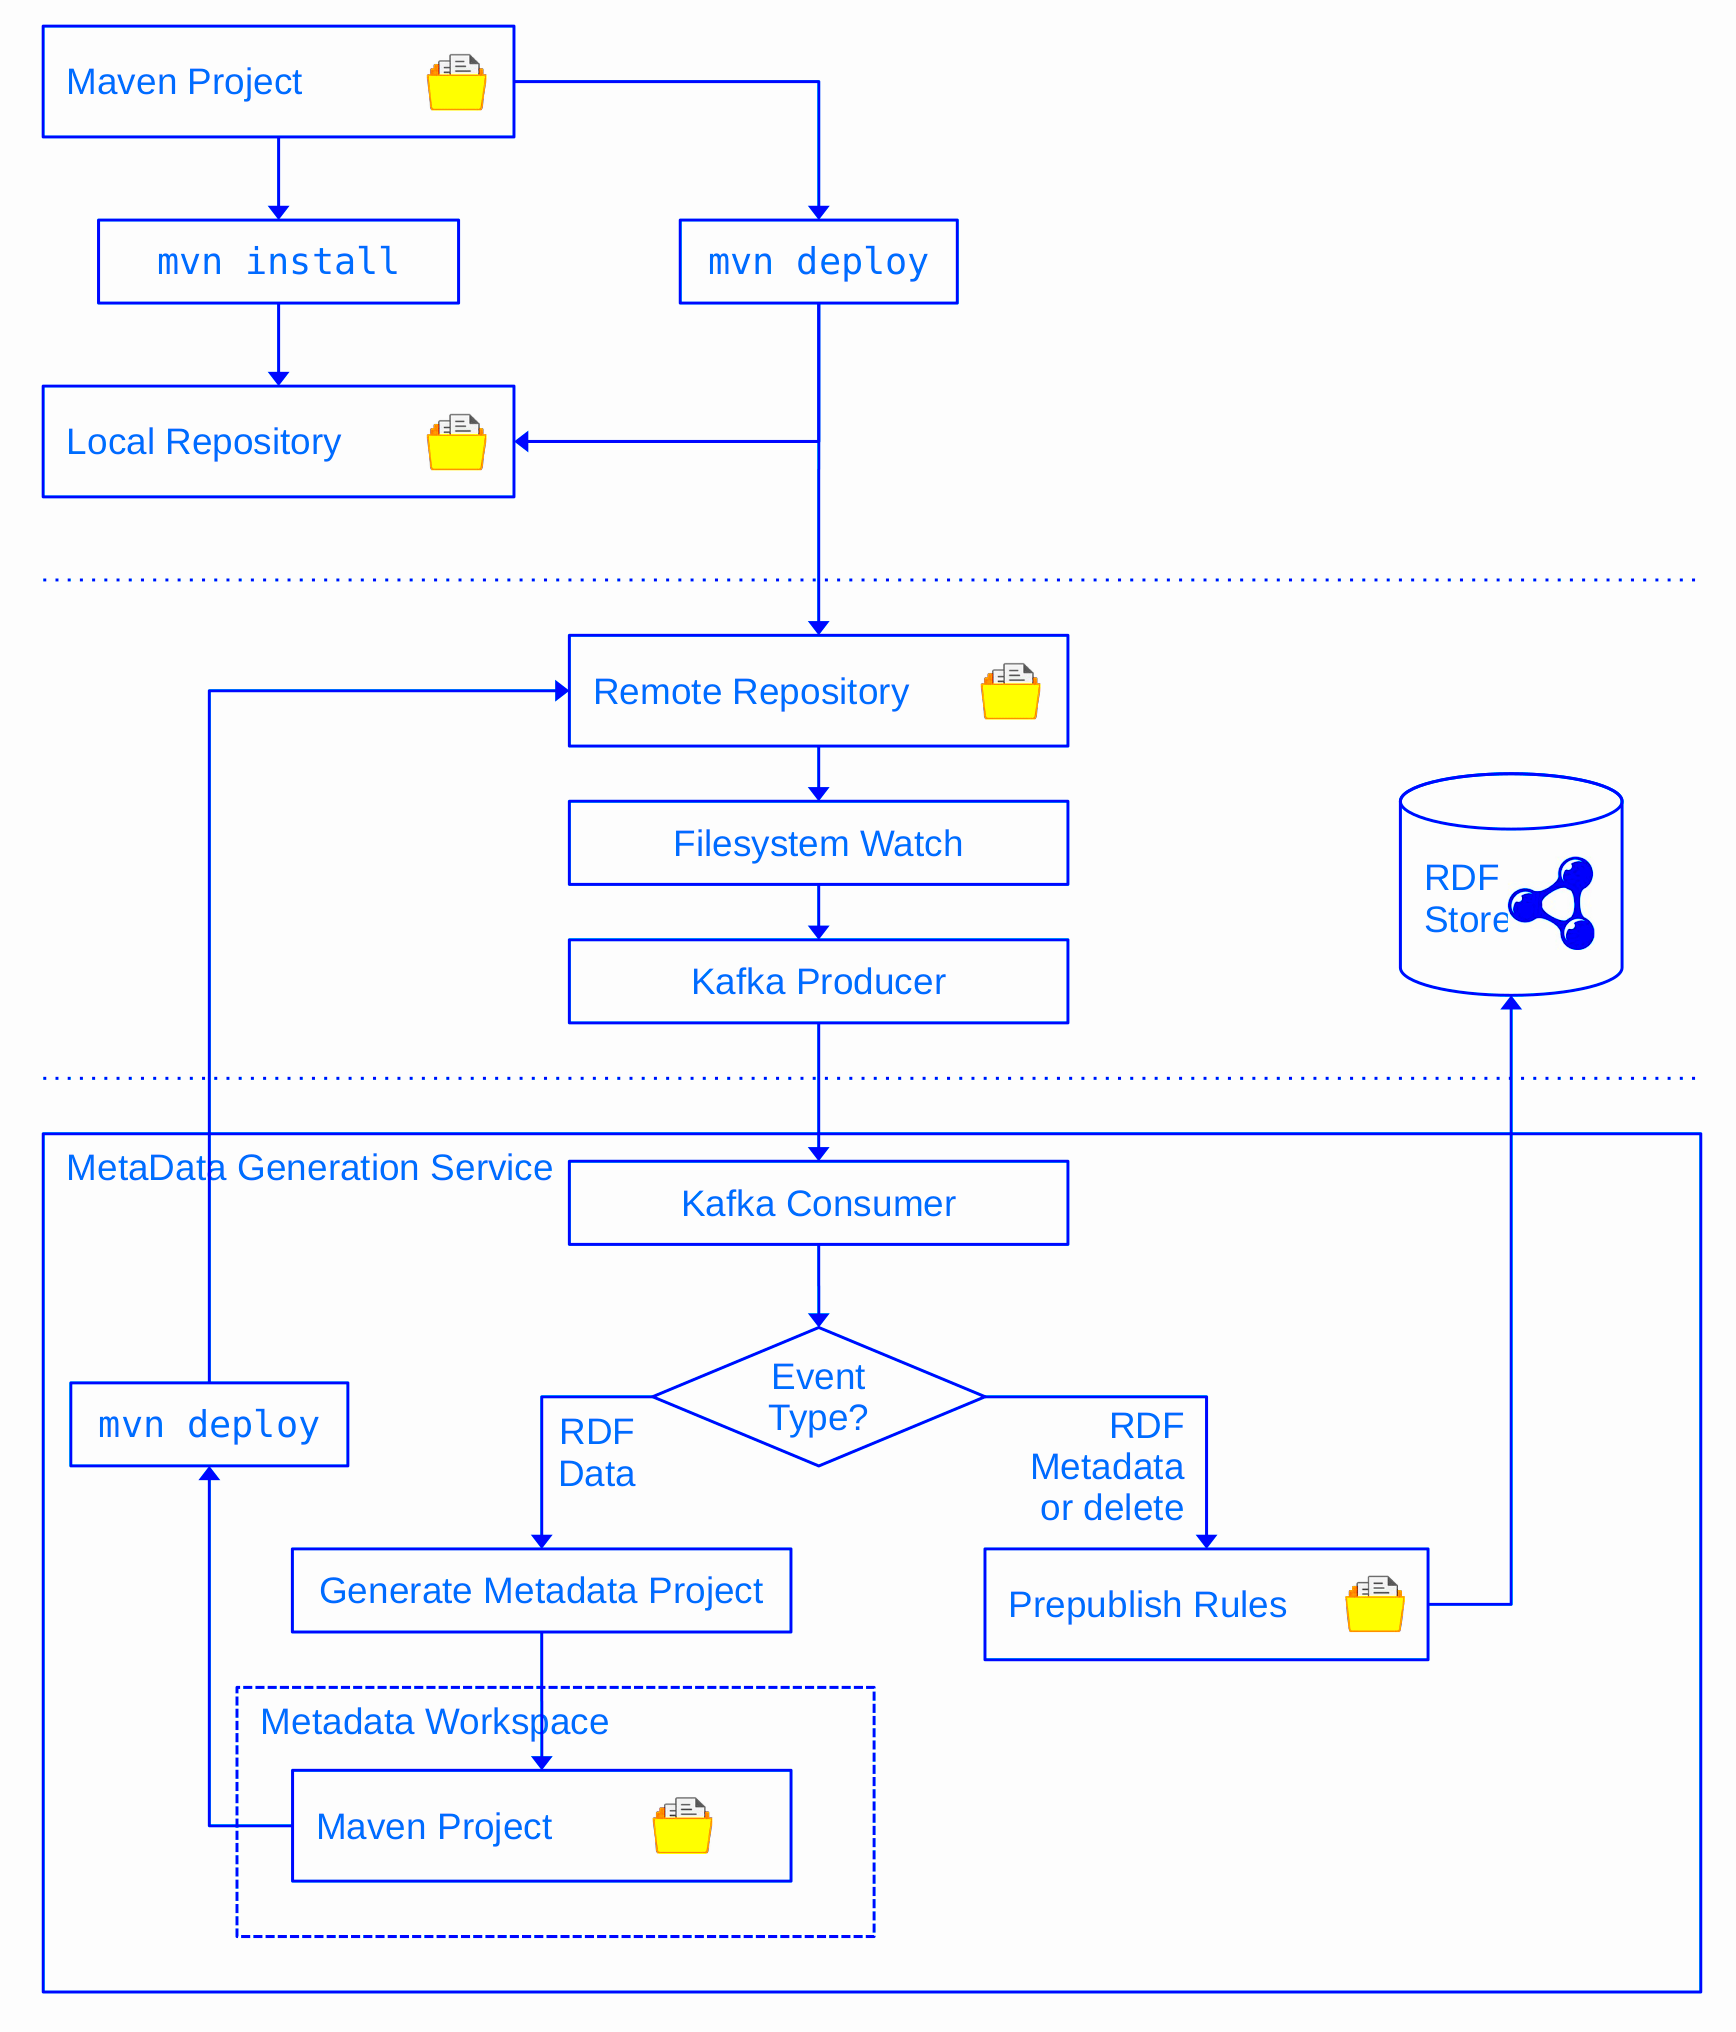
\includegraphics[width=0.7\textwidth]{images/2024-03-01-mvn-sync-architecture.png}
\caption{Architecture of our Maven-RDF-Sync approach.}
\label{fig:mvn-rdf-sync-arch}
\end{figure}
In the previous sections, we looked at how to build a Maven project that can deploy data.
In this section, we present \emph{mvn-rdf-sync}, an approach that after deployment of RDF data automatically generates and deploys metadata.
%VoID, PROVO and DCAT
The process is depicted in~\autoref{fig:mvn-rdf-sync-arch}.
%\todo{Add numbers to the picture}
The steps are:
\begin{enumerate}
\item A trigger on a Maven repository's file system detects changes and publishes appropriate events.
\item An event consumer examines the event type. If it is an RDF data artifact, then one or more Maven projects for metadata generation are created. This step essentially creates an instance from a Maven template project\footnote{\textls[-27]{\url{https://github.com/Scaseco/mvn-rdf-sync/blob/main/v3/dcat-generator/pom.xml}}}, using parameters from the changed artifact's POM.
By convention, we use the classifier \texttt{dcat} to indicate artifacts with DCAT metadata.
In principle, a future version of the setup could support attached RO-Crate files.
\item The metadata project is then deployed as usual using \texttt{mvn deploy}.
\item The change to the file system is detected and another event is sent.
\item This time the event consumer sees the RDF file with the \texttt{dcat} classifier and can choose the flow for publishing metadata.
In order to prevent arbitrary metadata to end up being published, metadata artifacts can be filtered by trusted groupIds.
\item A sequence of pre-publish rules, essentially SPARQL update queries, is used to transform the raw metadata into the final one. These rules are used to convert Maven URNs to resolvable download URLs and to run queries that for fixing any issues with previously published metadata.
\item Finally, the data ends up in the triple store for access. The metadata is loaded into a graph that matches the metadata artifact.
\item The data is now (publicly) accessible via SPARQL. Tools, such as Yasgui\footnote{\url{https://yasgui.triply.cc/}}, can be used to query and visualize the content.
\end{enumerate}

\begin{figure}[!htb]
\centering
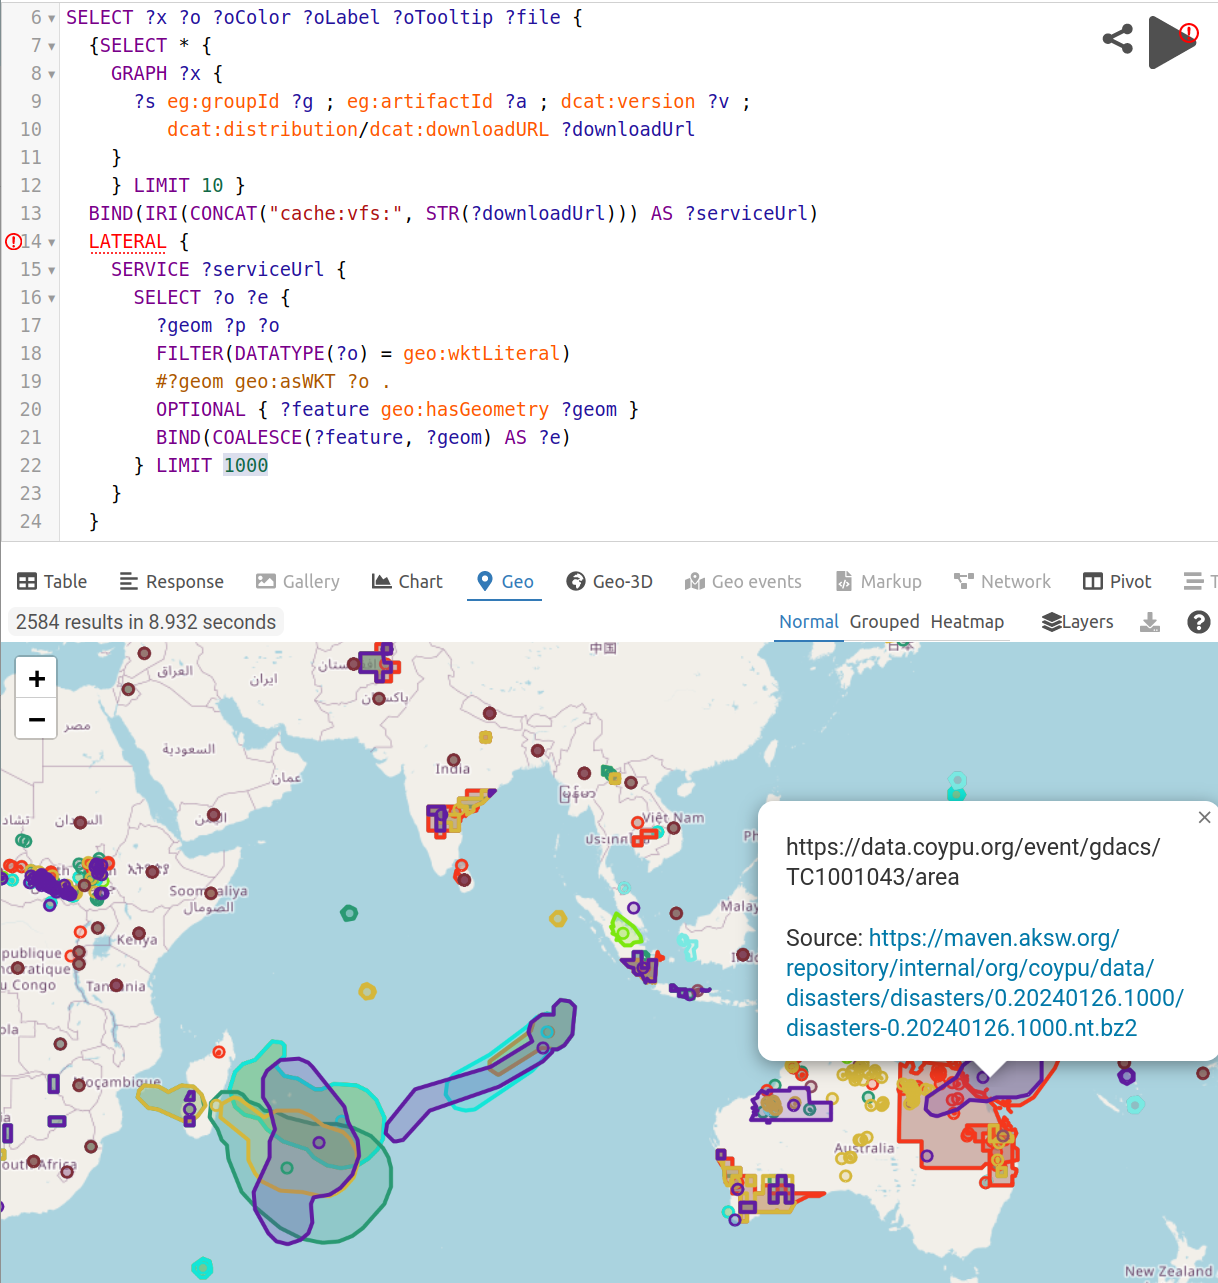
\includegraphics[width=0.8\textwidth]{images/Screenshot from 2024-03-18 01-11-50.png}
\caption{Visualization of data catalog content on a map via SPARQL.}
\label{fig:cat-content}
\end{figure}
%2024-03-03-yasgui-maven.png

A screenshot of our online demo\footnote{\url{https://scaseco.github.io/maven4data/online-demo.html}} is shown in~\autoref{fig:cat-content}.
It shows how the DCAT metadata in the triple store synchronized with the Maven repository can be queried with SPARQL and plotted on a map with Yasgui. As the mvn-rdf-sync process also generates VoID metadata, it is also possible to e.g. filter datasets by the used classes and properties. The datasets are identified by \texttt{urn:mvn:} URNs, such that a transfer of the repository to a different URL does not invalidate any dataset identifiers.

It is a design decision whether to use a single Maven template project to capture multiple metadata aspects, such as VoID, DCAT and PROV-O, or whether to maintain individual Maven templates for each of them. For the prototype we went with the former approach, but as the system grows it is likely that we will switch to the latter due to better modularity.
The metadata project includes generation of the provenance triples that state that the original artifact was generated by an activity whose plan is the URN of the original artifact's POM.
If that POM was designed to be self-contained then downloading the POM and running \texttt{mvn package} will re-run the build. If the POM was designed for reproducible builds then the output artifacts will match the deployed ones. For non-reproducible builds, such as those that consume live data from APIs, one should typically adjust the groupId and version appropriately before creating custom builds.

\section{Resources and Evaluation}
\label{sec:eval}
We have set up the \emph{Maven4Data} website with guides and examples that we have shown in this paper, demonstrating the effectiveness of the approach.

A relevant question is to what extent our mvn-rdf-sync approach degrades the performance of a filesystem-based repository due to overhead of file system watches. For this purpose we devised the ``repo-bench''\footnote{\url{https://github.com/Scaseco/mvn-rdf-sync/tree/main/benchmark}} benchmark:
We use a python script to generate a Maven project with $n=500$ sub modules, where each sub module has a corresponding RDF dataset. The triple count for the $i-th$ project is $i \times 1000$ triples, with $1 \leq i \leq n$, amounting to ${\frac{n}{2}} \times (n + 1) \times 1000 = 125.250.000$ triples in total with a size of 14.2G of data.

We measure the time it takes to install the poms with and without the file system watch active.
The experiment was carried out on a Dell XPS 9720 notebook with the following specs: CPU: Intel i9-12900HK CPU, SSD: NVMe PC801 NVMe SK hynix 2TB, RAM: 64GB.
We use the following basic watch to check for changes to the file system:

{\scriptsize
% too much detail/technical? (comment by sbin)
\begin{minted}{bash}
inotifywait "$HOME/.m2/repository" --recursive --monitor --format '%e %w%f' \
  --event CLOSE_WRITE --event DELETE | xargs -n 1 -P 0 bash -c 'echo  "$@"; sleep 1' _ {}
\end{minted}
}
The flag \texttt{-P 0} indicates to spawn a fresh process for each line emitted by inotifywait, such that maximum parallelism is utilized.
The finding is that regardless whether the following watch is active or not, running \texttt{mvn install} takes $\approx$20 seconds, which indicates that the watch itself does not impact the performance significantly. However, more extensive analysis is needed for how real-world workloads affect overall system performance.


%\todo{Evaluate and compare inotifywait with and without filter regex}


%\begin{minipage}{\linewidth}
%[language=yaml, caption=POM file for the creation of a TDB2 database.]

\section{Conclusions and Future Work}
\label{sec:conclusions}
This work is motivated by the multitude of solutions in the field of data management and the pursuit of a ``minimal'' one that is open source, can run locally, is extensible, and interoperable with Semantic Web technology.
% mature, file system based
In pursuit of such a solution, we took a deep dive in the Apache Maven ecosystem.
%we recapped the life cycle of data artifacts under an ETL process and showed that it can be mapped to the life cycle of Apache 
We presented a selection of use cases where the life cycle of data artifacts can be mapped to a Maven build process. A set of Maven plugins was devised for streamlining the generation of RDF and for the deployment of artifacts to CKAN instances.
We showed that Maven's build specifications can be designed in a way that makes them self-contained w.r.t. versioning, data processing and deployment.
The fact that upon deployment the POM is archived as well makes the process self-documenting and can be leveraged for reproducibility.
Based on our findings, we devised the \emph{mvn-rdf-sync} system, which listens to changes to Maven repository and triggers RDF metadata generation (via generated Maven projects) when RDF datasets are uploaded.
We assembled at the Website \emph{Maven4Data}
%\footnote{\url{https://scaseco.github.io/maven4data/}}
where we provide additional information and examples.
We also compared Maven to CWL and found that these systems are complementary: Maven's scope is more narrow than that of general workflow engines, yet it provides several features that are highly useful for versioning, packaging and deploying artifacts.

% both deployment of the output artifacts to different locations (WebDAV, CKAN) as well
%makes the data processing process self-contained.

Future work is along the following lines:
(1) Investigation of creating Research Object Crates from Maven.
%For example, would it make sense to build creates with Maven,interoperable with existing artifact repository systems.
(2) Analysing the feasibility of Maven plugins that can deploy to further popular public archives.
For (2), it needs to be investigated to what extent Maven's coordinate system can be bridged with the artifact naming system provided by those archives. For example, Zenodo provides APIs for custom tags which could be exploited for that purpose.
%and searching over them which could be exploited.

%\section*{Acknowledgments}
%The authors acknowledge the financial support by the German Federal Ministry for Economic Affairs and Climate Action in the project Coypu (project number 01MK21007A) and by the German Federal Ministry for Digital and Transport in the Project Moby Dex (project number 19F2266A).

%\pagebreak

%\bibliographystyle{splncs04}
%\bibliography{bibliography}





\end{document}
